% *******************************************************
% *******************************************************
%
% Copyright 2014 Benjamin Tovar Cisneros <https://github.com/TATABOX42>
%
% This program is free software; you can redistribute it and/or modify
% it under the terms of the GNU General Public License as published by
% the Free Software Foundation; either version 2 of the License, or
% (at your option) any later version.
%
% This program is distributed in the hope that it will be useful,
% but WITHOUT ANY WARRANTY; without even the implied warranty of
% MERCHANTABILITY or FITNESS FOR A PARTICULAR PURPOSE.  See the
% GNU General Public License for more details.
%
% You should have received a copy of the GNU General Public License
% along with this program; if not, write tfo the Free Software
% Foundation, Inc., 51 Franklin Street, Fifth Floor, Boston,
% MA 02110-1301, USA.
%
% *******************************************************
% contact: benjamin.tovarcis@gmail.com
% *******************************************************

% set document class
\documentclass[letter,12pt]{report}
% load document packages
\usepackage{class//thesis}
% load space package
\usepackage{setspace}

% *******************************
% set variables
% *******************************

	% set the author's name (First Middle ­Last ­Name)
	\newcommand{\authorName}{Javier de Velasco Oriol}
	% set the author's school program
	\newcommand{\schoolProgram}{Master of Science in Computer Science}
	% set the thesis name
	\newcommand{\thesisTitle}{
								MACHINE LEARNING AND DEEP LEARNING METHODS FOR LATE-ONSET ALZHEIMER'S DISEASE PREDICTION
	  					}

	% set the school name
	\newcommand{\schoolName}{Instituto Tecnológico y de Estudios Superiores de Monterrey}
	\newcommand{\schoolCampus}{Campus Estado de México}
	% set the department name
	\newcommand{\schoolDepartment}{School of Engineering and Sciences}
	% set school other details:
	\newcommand{\schoolPlace}{Atizapán de Zaragoza, E.M.}
	\newcommand{\thesisDate}{March, 2019}
	\newcommand{\thesisYear}{2019}
	% extra stuff
	\author{\authorName}
	\title{\thesisTitle}

	% *******************************
	% set variables for thesis committee 
	% *******************************

	% 1st adviser variables (Dr. First Middle ­Last ­Name)
	\newcommand{\firstAdvisorName}{Dr. Edgar Emmanuel Vallejo Clemente}
	\newcommand{\firstAdvisorSchoolName}{\schoolName}
	\newcommand{\firstAdvisorSchoolDepartment}{School of Medicine and Health Sciences}
	\newcommand{\firstAdvisorSchoolPlace}{\schoolPlace}

	% 2nd adviser variables (Dr. First Middle ­Last ­Name)
	\newcommand{\secondAdvisorName}{Dr. Jesús Karol Estrada Gil}
	\newcommand{\secondAdvisorSchoolName}{Biomarin Pharmaceuticals}
	\newcommand{\secondAdvisorSchoolDepartment}{Director, Statistical Genetics}
    \newcommand{\secondAdvisorSchoolPlace}{Novato, California, United States of America}

	% 3rd adviser variables (Dr. First Middle ­Last ­Name)
	\newcommand{\thirdAdvisorName}{Dr. Miguél González Mendoza }
	\newcommand{\thirdAdvisorSchoolName}{\schoolName}
	\newcommand{\thirdAdvisorSchoolDepartment}{\schoolDepartment}
    \newcommand{\thirdAdvisorSchoolPlace}{\schoolPlace}
	
	% 3rd adviser variables (Dr. First Middle ­Last ­Name)
	\newcommand{\fourthAdvisorName}{Dr. Enrique Hernández Lemus}
	\newcommand{\fourthAdvisorSchoolName}{Instituto Nacional de Medicina Genómica}
	\newcommand{\fourthAdvisorSchoolDepartment}{Subdirector, Population Genomics}
    \newcommand{\fourthAdvisorSchoolPlace}{Tlalpan, Mexico City}

	% Program director variables (Dr. First Middle ­Last ­Name)
	\newcommand{\programDirectorName}{Dr. Raúl Monroy Borja}
	\newcommand{\programDirectorRole}{Director of the Masters of Science Degree in Computer Science}

% *******************************************************
% *******************************************************
% Begin the document 
% NOTE: Do not move unless you want to change
% the order of chapters.
% *******************************************************
% *******************************************************

\begin{document}
	% import thesis cover: 
		\thispagestyle{empty} 
		%
% Copyright 2014 Benjamin Tovar Cisneros <https://github.com/TATABOX42>
%
% This program is free software; you can redistribute it and/or modify
% it under the terms of the GNU General Public License as published by
% the Free Software Foundation; either version 2 of the License, or
% (at your option) any later version.
%
% This program is distributed in the hope that it will be useful,
% but WITHOUT ANY WARRANTY; without even the implied warranty of
% MERCHANTABILITY or FITNESS FOR A PARTICULAR PURPOSE.  See the
% GNU General Public License for more details.
%
% You should have received a copy of the GNU General Public License
% along with this program; if not, write to the Free Software
% Foundation, Inc., 51 Franklin Street, Fifth Floor, Boston,
% MA 02110-1301, USA.
%

\begin{center}\large
    \textbf{\schoolName}\\
    \textbf{\schoolCampus}\\
    \textbf{\schoolDepartment}\\
\end{center}

%%%%%%%%%%%%%
\begin{center}
\end{center}
%%%%%%%%%%%%%

\begin{figure}[h!tb]
    \begin{center}
        
\includegraphics[width=0.7\columnwidth]{format/logo_TEC.png}
    \end{center}
\end{figure}

\begin{center}
    \textbf{\thesisTitle}
\end{center}

%%%%%%%%%%%%%
\begin{center}
\end{center}
%%%%%%%%%%%%%

\begin{center}
    \textbf{A thesis presented by:}
\end{center}

\begin{center}
    \textbf{\authorName}
\end{center}


%%%%%%%%%%%%%
\begin{center}
\end{center}
%%%%%%%%%%%%%

\begin{center}
    \textbf{Submitted to the
    School of Engineering and Sciences \\
    in partial fulfillment of the requirements for the degree of}
\end{center}

\begin{center}
    \textbf{\schoolProgram}
\end{center}

\null
\vfill

\begin{center}
    \textbf{\schoolPlace} 
\end{center}

\begin{center}
    \textbf{\thesisDate} 
\end{center}

 
		\newpage
	% load thesis committee:
		\thispagestyle{empty} 
		%
% Copyright 2014 Benjamin Tovar Cisneros <https://github.com/TATABOX42>
%
% This program is free software; you can redistribute it and/or modify
% it under the terms of the GNU General Public License as published by
% the Free Software Foundation; either version 2 of the License, or
% (at your option) any later version.
%
% This program is distributed in the hope that it will be useful,
% but WITHOUT ANY WARRANTY; without even the implied warranty of
% MERCHANTABILITY or FITNESS FOR A PARTICULAR PURPOSE.  See the
% GNU General Public License for more details.
%
% You should have received a copy of the GNU General Public License
% along with this program; if not, write to the Free Software
% Foundation, Inc., 51 Franklin Street, Fifth Floor, Boston,
% MA 02110-1301, USA.
%

\begin{center}\large
    \textbf{\schoolName}\\
    \textbf{\schoolCampus}\\
    \textbf{\schoolDepartment}\\
\end{center}

The  committee  members,  hereby,  certify  that  have  read  the  
thesis  presented  by \authorName\ and that it is fully 
adequate in scope and quality as a partial 
requirement  for  the  degree  of  \schoolProgram.


\begin{center}
        \textbf{THESIS COMMITTEE}
\end{center}


\begin{flushright}
        \vspace{0.25cm}
        \underline{\hspace{8cm}} \\ 
        % -------------------------
        \MakeUppercase{\firstAdvisorName} \\
        \firstAdvisorSchoolName \\
        \firstAdvisorSchoolDepartment \\
        \firstAdvisorSchoolPlace \\
        Co-Advisor 
        % -------------------------
\end{flushright}

\begin{flushright}
        \vspace{0.2cm}
        \underline{\hspace{8cm}}  \\
        % -------------------------
        \MakeUppercase{\secondAdvisorName} \\
        \secondAdvisorSchoolName \\
        \secondAdvisorSchoolDepartment \\
        \secondAdvisorSchoolPlace \\
        Co-Advisor 
        % -------------------------
\end{flushright}

\begin{flushright}
        \vspace{0.2cm}
        \underline{\hspace{8cm}} \\
        % -------------------------
        \MakeUppercase{\thirdAdvisorName} \\
        \thirdAdvisorSchoolName \\
        \thirdAdvisorSchoolDepartment \\
        \thirdAdvisorSchoolPlace \\
        Committee Member 
        % -------------------------
\end{flushright}

\begin{flushright}
        \vspace{0.2cm}
        \underline{\hspace{8cm}} \\
        % -------------------------
        \MakeUppercase{\fourthAdvisorName} \\
        \fourthAdvisorSchoolName \\
        \fourthAdvisorSchoolDepartment \\
        \fourthAdvisorSchoolPlace \\
        Committee Member 
        % -------------------------
\end{flushright}

\begin{center}
        \vspace{0.2cm}
        \underline{\hspace{8cm}} \\
        % -------------------------
        \MakeUppercase{\programDirectorName} \\
        \programDirectorRole \\
        \schoolDepartment
        % -------------------------     
\end{center}

\begin{center}
    \textbf{\schoolName}\\
    \textbf{\schoolPlace}, \textbf{\thesisDate} 
\end{center}


 
		%
% Copyright 2014 Benjamin Tovar Cisneros <https://github.com/TATABOX42>
%
% This program is free software; you can redistribute it and/or modify
% it under the terms of the GNU General Public License as published by
% the Free Software Foundation; either version 2 of the License, or
% (at your option) any later version.
%
% This program is distributed in the hope that it will be useful,
% but WITHOUT ANY WARRANTY; without even the implied warranty of
% MERCHANTABILITY or FITNESS FOR A PARTICULAR PURPOSE.  See the
% GNU General Public License for more details.
%
% You should have received a copy of the GNU General Public License
% along with this program; if not, write to the Free Software
% Foundation, Inc., 51 Franklin Street, Fifth Floor, Boston,
% MA 02110-1301, USA.
%

\thispagestyle{empty} % delete page number
\begin{center}
	\textbf{Declaration of Authorship}
\end{center}

	I, \authorName\, declare that this thesis titled, \thesisTitle\ and the 
	work presented in it are my own. I confirm that:

%%%%%%%%%%%%%
\begin{center}
\end{center}
%%%%%%%%%%%%%

\begin{itemize}
	\item This work was done wholly or mainly while in candidature for a research degree 
	at this University.
	\item Where any part of this thesis has previously been submitted for a degree or any 
	other qualification at this University or any other institution, this has been clearly 
	stated.
	\item Where I have consulted the published work of others, this is always clearly 
	attributed.
	\item Where I have quoted from the work of others, the source is always given. With 
	the exception of such quotations, this thesis is entirely my own work.
	\item I have acknowledged all main sources of help.
	\item Where the thesis is based on work done by myself jointly with others, I have 
	made clear exactly what was done by others and what I have contributed myself.
\end{itemize}

%%%%%%%%%%%%%
\begin{center}
\end{center}
%%%%%%%%%%%%%

\begin{flushright}
        \vspace{1 cm}
        \underline{\hspace{8cm}} \\ 
        % -------------------------
        \MakeUppercase{\authorName} \\
        \schoolPlace, \thesisDate
        % -------------------------
\end{flushright}

\null
\vfill

\begin{center}
	{@}\thesisYear\ by \authorName \\
	All rights reserved
\end{center}

\begin{center}
    \textbf{\schoolName}\\
    \textbf{\schoolPlace}, \textbf{\thesisDate} 
\end{center}
 
	% set the numeric indexing to be roman
		\pagestyle{headings}
		\setcounter{page}{1}
		\pagenumbering{roman}
	% load dedicatory page
		\section*{Dedicatory}
\textit{To my parents, for your unconditional love and support in all my life.
\\Thank you for the opportunity to follow my dreams and shoot for the stars.
\\To my Brothers, for every shared moment, fond memory and crazy ideas.
\\A man could not ask for a better family. I love you all with all my heart.
\\
\\
To Vale, you complete my life. Thank you three thousand times to the moon and back.
\\Le melithon anuir, my Sun and Stars.
\\
\\Journey before Destination.
}



	% load acknowledgments page
	  \section*{Acknowledgments}

I thank my co-advisor \firstAdvisorName, for his extraordinary guidance and assistance throughout the Master Degree, for taking me into the wonderful world of Bioinformatics, for his dedication to this project, and for giving me a thesis project that I am truly passionate about. This thesis would not exist without him.\\

I thank my co-advisor \secondAdvisorName, for teaching me so much about Genetics, Statistics and Quality Control, for giving me very valuable feedback and pointers to guide me, and for his constant dedication to this project. This thesis would not be as thorough nor clean without his assistance.\\

I thank Dr. José Gerardo Taméz Peña, for the development of the FRESA.CAD Benchmark and his assistance in applying the benchmark to the datasets, and for the work we have developed together.\\

I thank Dr. Claudia Marquez-Luna, for the development of the LDPred-funct method and for her assistance in applying it to the datasets.\\

I thank the committee members \thirdAdvisorName  and \fourthAdvisorName, for taking the time to provide valuable time in the thesis defense procedure and for their comments and feedback to make this thesis as complete and correct as possible.\\

I thank my degree Co-ordinator \programDirectorName, for providing support and guidance across the Masters Degree and further career choices.\\

I thank the Tecnologico de Monterrey for the resources and infrastructure provided that supported the development of this thesis. I also thank it for the scholarship provided to cover tuition fees across the degree period.\\

I thank the Consejo Nacional de Ciencia y Tecnología (CONACYT) for the scholarship and funding during the period I dedicated to the Masters Degree, and in general for supporting the development of science in Mexico.\\

I thank our colleagues from the Bioinformatics for Clinical Diagnosis Research Program, School of Medicine and Health Sciences, Tecnologico de Monterrey, for their valuable comments on this work. \\


I thank the Alzheimer's Disease Neuroimaging Initiative for providing the Whole-Genome Sequence data used in this project. Data collection and sharing for this project was funded by the Alzheimer's Disease Neuroimaging Initiative(ADNI) (National Institutes of Health Grant U01 AG024904) and DOD ADNI (Department of Defense award number W81XWH-12-2-0012). ADNI is funded by the National Institute on Aging, the National Institute of Biomedical Imaging and Bioengineering, and through generous contributions from the following: AbbVie, Alzheimer’s Association; Alzheimer’s Drug Discovery Foundation; Araclon Biotech; BioClinica, Inc.; Biogen; Bristol-Myers Squibb Company; CereSpir, Inc.; Cogstate; Eisai Inc.; Elan Pharmaceuticals, Inc.; Eli Lilly and
Company; EuroImmun; F. Hoffmann-La Roche Ltd and its affiliated company Genentech, Inc.; Fujirebio; GE Healthcare; IXICO Ltd.; Janssen Alzheimer Immunotherapy Research \& Development, LLC.; Johnson \& Johnson Pharmaceutical Research \& Development LLC.; Lumosity; Lundbeck; Merck \& Co., Inc.; Meso Scale Diagnostics, LLC.; NeuroRx Research; Neurotrack Technologies; Novartis Pharmaceuticals Corporation; Pfizer Inc.; Piramal Imaging; Servier; Takeda Pharmaceutical Company; and Transition Therapeutics. The Canadian Institutes of Health Research is providing funds to support ADNI clinical sites in Canada. Private sector contributions are facilitated by the Foundation for the National Institutes of Health (www.fnih.org). The grantee organization is the Northern California Institute for Research and Education, and the study is coordinated by the Alzheimer’s Therapeutic Research Institute at the University of Southern California. ADNI data are disseminated by the Laboratory for Neuro Imaging at the University of Southern California.\\

I thank the International Genomics of Alzheimer's Project (IGAP) for providing summary results data for these analyses. The investigators within IGAP contributed to the design and implementation of IGAP and/or provided data but did not participate in analysis or writing of this report. IGAP was made possible by the generous participation of the control subjects, the patients, and their families. The i–Select chips was funded by the French National Foundation on Alzheimer's disease and related disorders. EADI was supported by the LABEX (laboratory of excellence program investment for the future) DISTALZ grant, Inserm, Institut Pasteur de Lille, Université de Lille 2 and the Lille University Hospital. GERAD was supported by the Medical Research Council (Grant n 503480), Alzheimer's Research UK (Grant n 503176), the Wellcome Trust (Grant n 082604/2/07/Z) and German Federal Ministry of Education and Research (BMBF): Competence Network Dementia (CND) grant n 01GI0102, 01GI0711, 01GI0420. CHARGE was partly supported by the NIH/NIA grant R01 AG033193 and the NIA AG081220 and AGES contract N01–AG–12100, the NHLBI grant R01 HL105756, the Icelandic Heart Association, and the Erasmus Medical Center and Erasmus University. ADGC was supported by the NIH/NIA grants: U01 AG032984, U24 AG021886, U01 AG016976, and the Alzheimer's Association grant ADGC–10–196728.





%%%%%%%%%%%%%
\begin{center}
\end{center}
%%%%%%%%%%%%%

\begin{flushright}  
	\MakeUppercase{\authorName}
\end{flushright}  

\begin{center}
    \textbf{\schoolName}\\
    \textbf{\schoolPlace}, \textbf{\thesisDate} 
\end{center}

	%%%%%%%%%%%%%%%%%%%%%%%%%%%%%%%%%%%%%%%%%%%%%%%%%%%%%%%%%%%%%%%%%%%%%%%%%%%%%%%%
	% include abstract
		% ***************************************
% ***************************************
\chapter*{Abstract} \label{abstract}
\addcontentsline{toc}{chapter}{Abstract}
% ***************************************
% ***************************************

\begin{center}\large
    \textbf{\thesisTitle}\\
\end{center}

%%%%%%%%%%%%%
\begin{center}
\end{center}
%%%%%%%%%%%%%

\begin{center}
    \authorName\\
    \schoolName, \thesisYear\\
\end{center}

\begin{center}
    Co-advisor: \firstAdvisorName\\
    Co-advisor: \secondAdvisorName\\
\end{center}


%%%%%%%%%%%%%
\begin{center}
\end{center}
%%%%%%%%%%%%%






Alzheimer's disease (AD) is the leading form of dementia. This disease represents a heavy burden in families worldwide, as there is currently no cure, requires constant care and is highly correlated with increasing age. Over 25 million cases have been estimated worldwide and this number is predicted to increase two-fold every 20 years. Even though there are a variety of clinical markers available for the diagnosis of AD, the accurate and timely diagnosis of this disease remains elusive, and this detection can be too late to start planning or testing experimental treatments. Thus, a system that can reliably detect the formation of Alzheimer's years before symptoms begin to show could help identify individuals at risk that could benefit from these treatments. Recently, over a dozen of genetic variants predisposing to the disease have been identified by genome-wide association studies. However, these genetic variants only explain a small fraction of the estimated genetic component of the disease. Therefore, useful predictions of AD from genetic data could not rely on these markers exclusively as they are not sufficiently informative predictors. This Master in Computer Science thesis is aimed towards expanding the state of the art in the use of machine learning and deep learning algorithms to predict the genetic risk of Alzheimer's Disease by using a larger number of genetic variants. Experimental results indicate that the proposed models holds promise to produce useful predictions for clinical diagnosis of AD.


	% list of figures
		\listoffigures
		\addcontentsline{toc}{chapter}{List of Figures}
		\newpage
	% list of tables
		\listoftables
		\addcontentsline{toc}{chapter}{List of Tables}
		\newpage
	% Index of contents
		{\pagestyle{plain}
		\tableofcontents
		\cleardoublepage}
		\newpage
	%%%%%%%%%%%%%%%%%%%%%%%%%%%%%%%%%%%%%%%%%%%%%%%%%%%%%%%%%%%%%%%%%%%%%%%%%%%%%%%%
	% change the numeration of pages to Arabic starting from number 1
		\pagestyle{headings}
		\setcounter{page}{1}
		\pagenumbering{arabic}
		\newpage
	%%%%%%%%%%%%%%%%%%%%%%%%%%%%%%%%%%%%%%%%%%%%%%%%%%%%%%%%%%%%%%%%%%%%%%%%%%%%%%%%

	% set space to one and half spacing:  
	\onehalfspacing

	% import text:
	% ********************** PART 1
		% ***************************************
% ***************************************
\chapter{Introduction} \label{introduction}
% ***************************************
% ***************************************

Alzheimer Disease is a neurodegenerative disease that causes the brain to start degrading, it is characterized by the loss of cognitive abilities such as memory, reasoning, language and behavior. The disease leads to dementia and ultimately to death. Late-onset Alzheimer's disease (LOAD) is the most common form of dementia (60\% -- 80\% cases). It occurs more often in people age 60 and older. 

This is a chronic disease which currently has no know effective therapeutic treatment for the disease, either to stop the advance of the sickness or reverse the damage caused by it. The reduced amount of medication available only helps with managing the symptoms to slightly improve quality of life. An estimate from \cite{Ballard2011}  shows that Alzheimer Disease affects between 4 and 6 percent of the population over 65 years old, with an estimated 2 million deaths per year a high maintenance cost.

There is no single effective clinical test for LOAD. Currently, a confirmatory diagnosis of the disease is exclusively available from pathological postmortem examinations \cite{SHAO20171}. However, there is a collection of tests that are considered useful predictors for the clinical diagnosis of LOAD, such as cognitive tests, cerebrospinal and blood biomarkers, genetic markers, and MRI/PET images\cite{Li2017}. Magnetic Resonance Images (MRI) are taken of multiple regions of the brain through the use of magnets and are then analyzed by algorithms or doctors for telltale signs of Alzheimer's Disease progression inside the structure of the brain (Mainly looking for lower than normal size in the temporal and parietal lobes). Positron Emission Tomography (PET) scans use radiotracers linked to biomarkers of the disease to understand and observe the concentration of these biomarkers in specific regions of the brain.
\newpage
Unfortunately, the majority of these clinical markers are strongly correlated with the progression of this disease, meaning that they would typically be more informative at later stages of the disease or are very expensive to perform on large population screens. Better clinical tests are needed which are capable to provide accurate predictions for the early diagnosis of LOAD. In effect, it is expected that experimental therapeutic and palliative interventions will be more effective at earlier stages of the disease \cite{biogen2016}.

A promising alternative for the prediction of LOAD is through genetic testing. For example, specific alleles of Apolipoprotein E (APOE) have been implicated as the largest genetic risk factors for LOAD. However, the use of the APOE $\epsilon4$ in clinical practice has been controversial. For example, even though the odds ratio of this genetic marker has been estimated at over 3, in practice, only 1 of 4 patients with this allele progresses to the disease. In the end, there is no known ultimate cause of LOAD and it is likely that LOAD is a complex disease whose etiology is driven by both environmental and multiple genetic components \cite{PANPALLIATES2016124}.

Recent advances on genome technologies have enabled the identification of several genetic variants that are associated with complex diseases \cite{Manolio2009} \cite{MacArthur2017}. However, the complete understanding of the genetic architecture of most complex diseases has remained elusive \cite{Ridge2013}. Advances in this area hold the potential to contribute to the identification of novel drug targets for LOAD \cite{Estrada2018}\cite{Freudenberg2018}.

The genetic component of LOAD has been estimated to be 79\%. However, recent studies on the heritability of LOAD have estimated that common genetic variants identified by genome-wide association studies (GWAS, check chapter 2.1 page \pageref{GWAS}) are only capable to explain 33\% of the phenotypic variance. This means that over 40\% of the genetic component remains unexplained \cite{Raghavan2017}. One such example of a complex genetic phenotype is human height. When using GWAS to obtain specific SNPs researchers could not predict height precisely, as those markers could only explain a fraction of the genetic component. Instead, researchers used multiple common variants (250,000+ SNPs) and were much more succesful in explaining the genetic variation \cite{Yang2010}.

Recent studies have been postulated a collection of theories that should be capable to explain the missing heritability (Check chapter 2.1 page \pageref{missHerit}) of complex diseases \cite{Manolio2009}\cite{Eichler2010}. These theories include: (1) a more comprehensive collection of genes with low effect sizes associated with the disease; the existence of gene-gene interactions --epistatic effects; and gene-environmental interactions, among others.
\newpage
For Artificial Intelligence this problem presents an opportunity to develop an algorithm that can take the $\beta$-Amyloid hypothesis (For more information check chapter 2.2 page \pageref{betaAmyloid}) as well as yet-unexplored genes using Machine Learning. These models can discover genetic features as well as correlations that can be used to analyze and create predictions based on a learned model of the chances a person might have of developing Alzheimer disease. The person would go to a clinic where tests would be taken to obtain the genetic information, which would then be analyzed by the machine learning models. After processing them the system would give a good estimate of the risk this person has of developing Alzheimer's Disease. This has the possibility to have sizable impact as currently the amount of people living over 65 years is constantly increasing, which in turn means that more people will start to develop Alzheimer and will require both care and attention. 150 million people are expected to develop this disease by 2050 and as such it will be quite expensive in terms of family and resources to handle this disease. While this technology is purely predictive this method can have the benefit to prepare and plan economically, socially and emotionally for the effects of Alzheimer. Additionally, if a preemptive medicine can be shown to reduce $\beta$-Amyloid plaque formation before Alzheimer develops such a technique would be required to determine who should receive these medications to slow and hopefully prevent Alzheimer disease. Another possible avenue would be using the genetic knowledge to design specific drugs targeted to those exact mutations; with tools such as monoclonal antibodies, small bodies or gene therapy. Finally, with the development of CRISPR-CAS9 and other gene-manipulating methods it could be possible in the future to adjust the genes responsible for increasing the risk of Alzheimer's Disease.

An approach using Deep Neural Networks (Check chapter 2.3 page \pageref{DNNs}) for learning is the main component of the Artificial Intelligence solution. Deep Learning has developed into maturity in the latest years thanks to both higher processing power and the creation of frameworks that optimize working with it. Deep Learning allows the detection of slight and tiny patterns \cite{Schmidhuber2015}, which to a human doctor would be invisible, to use for predicting a probability regarding the development of Alzheimer in future years\cite{Jessen2014}. 

To contrast the Deep Learning model two more Machine Learning methods are used: Random Forest and Support Vector Machines (Check chapter 2.3 page \pageref{RF}) . Random Forests have been used in genomics \cite{CHEN2012323} and thanks to the statistical properties of the ensemble model can find a larger group of interesting features useful for multi-gene approaches. Support Vector Machines have also been used with success in genetic micro-arrays \cite{peng2003molecular}, and could be useful as the hyper-plane model and the kernel trick could allow it to find non-linearity compositions between multiple genes.

Considering the limitations in size of the ADNI dataset, to assess the performance of the Deep Learning method in an ideal case a complex genetic disease similar to Alzheimer's is simulated and evaluated. This is done to measure the impact of the dataset size with respect to the classifier performance and doing cross-analysis with respect to the number of variants used to classify. Apart from the simulation, an artificial data augmentation procedure is also implemented to increase the size of the ADNI dataset for training the models in a way that allows to compare how the procedure could manage to perform if the ADNI dataset was larger.

Additionally, the FRESA.CAD (Feature Selection Algorithms for Computer Aided Diagnosis, check chapter 2.3 page \pageref{fresaCAD}) \cite{fresa} benchmark tool is further used to perform a statistical feature selection using the BSWiMS method, LASSO, KNN, as well as the ensemble of the models. The cross-validation and repetition methods also give it a high degree of statistical accuracy. FRESA.CAD additionally has the advantage of returning the features most selected across the models and as such can extrapolate to a valid analysis of the gene variants which in the end allows a more direct interpretation.

To contrast Machine Learning methods with a more traditional approach to genomics methods, the LDPred-funct algorithm by Dr. Marquez-Luna \cite{Marquez-Luna375337} is also used to generate a Polygenic Risk Score (Check chapter 2.1 page \pageref{PRS})  and classify the dataset.

A series of experiments are conducted using these methods for predicting late-onset Alzheimer's disease using Whole Genome data from the Alzheimer's Disease Neuroimaging Initiative (ADNI) project. The mixture and variation between experiments gives a rounded analysis of the classification problem, it's complexity as well as a confidence of the results obtained using the different methods.


Experimental results indicate that classification performance of $\sim$ 65\%~$\sim$ 70\% of area under the ROC curve (AUC) can be achieved with the proposed Machine Learning models. Furthermore, the experiments reported here suggest that an increasing number of genetic variants hold the potential to contribute to improve the predictive capabilities of the proposed model providing that sufficiently large datasets are available.
\newpage
% *******************************************
\section{Justification} \label{justification}
% *******************************************

Alzheimer disease as it has been shown is a complex disease with multiple components and that is not yet understood. Thus initially the problem begins at the stage where possible solutions must base themselves on a tenuous hypothesis regarding what precisely leads to Alzheimer. The disease is not yet understood as sufficiently as required to realize a quite accurate and precise solution. 

Currently there does not exist a sure-proof and financially viable way to detect Alzheimer before symptoms begin to happen, as Laske describes \cite{LASKE2015561}. Most of the time either the disease goes undetected or is diagnosed via mental and analytic exams done on a patient who is already experiencing the symptoms. These tests measure cognitive functions and memory capabilities to try and diagnose Alzheimer, and indeed are quite accurate with the corresponding diagnosis. But the problem lies in that these tests come in too late to be of help for mid and long term planning or for potential treatments that might slow down the progression of Alzheimer. Another problem with tests is that there is no method that can work en-masse cheaply so that everyone above 60 takes them consistently. As Laske mentions \cite{LASKE2015561} there are some interesting avenues such as  gait and speech analysis, blood-based biomarkers and computational models.

Genetic tests as shown before can also be undertaken to find the presence of known genes that increase the risk of developing Alzheimer, but as is the current case there is no definitive result using single markers.

This problem has been analyzed by multiple institutions and one organization in particular has created a database to study and research Alzheimer disease: The Mark and Mary Stevens Neuroimaging and Informatics Institute. Together with other institutions they have created the Alzheimer’s Disease Neuroimaging Initiative (ADNI) database \cite{MarkandMaryStevensNeuroImagingInstitute} which consists of studies taken of multiple American cohorts. These subjects have taken Cerebrospinal Fluid(CSF) and Positron Emission Tomography (PET) to detect $\beta$-Amyloid and tau proteins, Magnetic Resonance Imaging (MRI) of specific brain areas, Whole-Genome sequencing as well as multiple cognitive assessment tests and finally a medical diagnostic of the mental condition. This is a complete database with multiple tests taken across the years on the same subjects to analyze and record progression and as such is the database being used for training the machine learning algorithms. 
\newpage
There have been some approaches to detect and predict Alzheimer based on the use of Support Vector Machines \cite{Orru2012} and MRI analysis \cite{Kloppel2008}\cite{Long2017}. The problem with the first solution is that Support Vector Machines enrich the data artificially and can be subject to over-fitting on a data set. The second one requires costly and lengthy MRIs which makes the cost prohibitively more expensive such as to use them in a genetic test done just once.

Thus a solution that is scalable, generalizable and precise is required to solve the problem of successfully predicting the probability of developing Alzheimer in a precise manner.

Deep learning (DL) are machine learning models that are becoming increasingly popular in solving a variety of problems in medicine \cite{LeCun2017}.  Deep learning is an extension of the Neural Network algorithm, where the amount of layers is greatly increased. When this schema is complemented with processing power and representative data-sets it allows the agent to learn the representation of the date, and create multiple levels of it. Thanks to this the agent not only detects interesting features and crucial information, but it also has a limited knowledge of how an object or concept is represented across the multiple dimensions that create it. It does this without any hand-crafted features or details, thus being great at handling new data and requiring little fitting. In recent years, DL models have shown excellent results on the examination of clinical images, approaching human level performance \cite{Esteva2017}. Thus it can be worthwhile to explore the use of dense deep neural networks (DDNN) models for predicting complex disease from genetic data.

Through the observation of the ADNI data set the deep network will be able to learn a model that can successfully and accurately predict the probability of having Alzheimer in the future. This is without having the full spectrum of biological information and the concrete model of disease progression. The neural networks will learn dynamically what variants cause Alzheimer to develop further in the future and given incomplete data from a new patient to estimate the development (or a lack thereof) of Alzheimer disease. The proposed neural networks will correctly determine whether a given patient fits into either class of the binary classification and with which probability they belong to that category. The algorithm will continually improve itself via backpropagation to ensure future predictions are as accurate as possible and to get a more clear grasp of the true underlying model of Alzheimer disease progression. 
\newpage
Equally, Random Forest and Support Vector Machines are also robust machine learning techniques that perform well in small datasets and which do not require as many samples as other methods to generate good results. As such it is worth contrasting with the deep network due to the size of the ADNI. The downside with these methods is that the continuous improvement for the system by feeding additional samples is not as straightforward and robust as the deep network. Additionally, if the true underlying model is much more complex and non-linear than expected then it is possible that the deep network is the method that can describe it more fully.

The simulation analysis is a useful tool to validate some underlying thoughts about the method. Firstly, it allows the replication of a complex genetic disease with models that are based on human genetics, thus creating a valid dataset to prove how these methods work in genetic phenotype prediction. This in turn allows the use of much larger sample sizes, and gives perfect testing grounds to analyze the effect of increasing the sample size for deep learning and the other machine learning methods. It also allows testing the effect of increasing both the sample size and the number of variants used to calculate the risk. The only limitation with this method is that the simulated diseases are completely genetic in nature, while Alzheimer's is only partially genetic, and as such the maximum scores achievable between them are not the same.

Furthermore, the inclusion of the artificial data augmentation method is also highly beneficial to further analyze the two previous points regarding the increase in the dataset size as well as the number of variants used with the real world dataset. By being able to generate more samples based on a real-world dataset the statistical distributions, allele frequencies and other genetic components of the simulated samples closely follow those that exist in the ADNI. As such, allowing for a simulation that is much more robust, follows the same characteristics of existing samples and can be directly used for the disease that is of interest. Additionally, the method also allows a purely synthetic training to be validated on the real-world samples. This is worthwhile due to the fact that genetic datasets are not very common and they tend to have a reduced number of samples, in contrast with imaging tasks with millions of images further augmented to have even more.

By using the FRESA.CAD Benchmark the feature analysis is incorporated which allows the system to predict which variants are the ones that give the most information, which are the ones being chosen the most, and the prediction capability of each gene. Using these results it is possible to analyze the variants responsible for increasing the risk of Alzheimer's disease and which are useful in a prediction algorithm. With this the amount of genes than need to be genotyped is reduced drastically, and chipsets with the desired genes can be chosen. Additionally, biological and chemical pathways of the variant can be analyzed to confirm if the gene correlation is not only statistical but has a biological relationship with Alzheimer's. The machine learning methods in the FRESA.CAD benchmark also have a robust statistical analysis and as such could provide correct predictions and a certainty of them.

The proposed methods are both scalable and generalizable, while being efficient when processing vast amounts of data and stable when facing outliers, coupling this with inherent learning will make it affordable.


% *******************************************
\section{Hypothesis} \label{hypothesis}
% *******************************************

In this thesis, it is proposed to explore the hypothesis on the existence of multiple genes with low effect sizes contributing to the risk of developing LOAD. To test this hypothesis it is proposed to conduct computational experiments on the ADNI dataset by the construction of deep learning and machine learning predictive models using large collections of genetic markers that are capable to predict LOAD from this data and which obtain a score above 65\% in the ROC AUC Score for the binary classification problem. Furthermore, it is also proposed to validate these models on a simulated dataset to benchmark the performance of these algorithms on a general complex genetic disease to prove the general validity of the models, as well as running the data-augmentation method to validate the performance of the models using a larger dataset. Finally, it is proposed to perform tests using the FRESA.CAD Benchmark for feature analysis to identify the gene variants associated with the prediction capability.  
\newpage
The main questions to be solved in this hypothesis are the following:
\begin{itemize}

\item What are the optimal tuning parameters for the Deep Networks and Machine Learning models that can minimize the cost function and obtain the best receiver operating characteristic curve for the described task?

\item What is the performance of these same algorithms when using a simulated complex disease instead of a real-world dataset?

\item What is the benefit of using a data augmentation method to artificially increase the genetic dataset?

\item Does the data set contain enough data and diversity so that the different models can extract good representations and provide real world solutions?

\item Which gene variants and data representation are the ones that provide the most information for prediction?
\item What are the limitations and improvements of the proposed systems for prediction under the described hypothesis?

\end{itemize}

% *******************************************
\section{Objectives} \label{objectives}
% *******************************************

The main objective to accomplish with this thesis is to prove that the proposed Deep Learning and Machine Learning methods trained with the simulations as well as the ADNI data set can be used reliably to accurately predict the risk of developing Alzheimer disease of an individual. This will be proved in tests by obtaining high sensitivity and specificity to achieve an area under the ROC curve of 0.65 or more in multiple test sets. One secondary objective to accomplish is to prove that the model works correctly and maintains a high degree of precision if the data it is given is limited or noisy as is the case with multiple sequencing datasets. This will be validated via the use of multiple samples which have data missing. Another objective is to ensure that this method can be applied to real life scenarios and not only simulated scenarios, by using data obtained from real patients obtained in the ADNI dataset which consists of real patients and analysing the results obtained there in addition to the simulated experiments. The last goal to accomplish is to ensure that the system can be implemented and executed in an affordable manner which can be easily scaled to benefit a considerable amount of the population. This will mostly depend on the chosen variants  which are necessary to increase the ROC metric and their attached cost as not all gene variants can be genotyped as easily or using the same chipset.                  



% *********************************************************
\section{Thesis contributions} \label{thesis_contributions}
% *********************************************************

The thesis, through the different experiments obtains multiple results from varied methods and as such the results show how some methods or techniques are better suited to the current problem (And the greater problem of Machine Learning for Genomics Analysis and Diagnostic) and which others do not perform greatly. 

The main contributions of this thesis to the state of the art are as follows:

\begin{itemize}
	\item First implementation of Deep Learning using Whole-Genome Sequencing data for Alzheimer's Disease risk prediction.
	\item Comparison and bench-marking between different Machine Learning methods for the classification task.
	\item Analysis of the methods that performed adequately on the task.
	\item Simulation of a complex genetic disease and respective performance of the same algorithms on the simulation.
    \item Data augmentation procedure for enrichment of genetic datasets using a valid statistical basis.
    \item Feature variant selection and Meta-Analysis through the use of FRESA.CAD for identification of the important variants for a clinical diagnosis and solution.
    
\end{itemize}


% ***************************
\section{Thesis organization}
% ***************************

The organization of this thesis is as follows: Chapter \ref{background} introduces to basic concepts in the area of Machine Learning, Deep Learning, Alzheimer's Disease and Genomics, as well as work done previously in the area. In chapter \ref{materials_and_methods}, the materials and methods are shown. This chapter comprises the source and describes each dataset employed, as well as the methodology behind the experiments. The results, experiments and  discussion are shown in chapters \ref{results}. Finally, the document ends with the conclusions and future work in chapter \ref{conclusions}.









		% ***************************************
% ***************************************
\chapter{Background} \label{background}
% ***************************************
% ***************************************
In this chapter the background knowledge useful to understand this thesis is described as well as the previous work done by other scientist in the area to give an overview of what has been done previously and how this research advances it. The first section will describe the basics of Genomics applied to LOAD, as well as the main tools and procedures used to generate, process and evaluate the dataset. Afterwards, a more in-depth description of Alzheimer's disease and the factors that make it up and possible causes is given.  The next section will describe the basics of Machine Learning as well as the methods used in this thesis: Support Vector Machines, Random Forest, Neural Networks and Deep Networks, and the FRESA.CAD Benchmark.  Finally, the research done with Machine Learning for the prediction of genetic diseases, the detection of Alzheimer's and the prediction of Alzheimer's is shown.

\section{Genomics}

Genomics is the study of the genome of individuals or species. The genome encodes the genetic information across different chromosomes, which in turn can be divided in functional units of genes made up of a varying number of base pairs. These base pairs are the building blocks of the entire genome, and a single mutation can have a strong enough impact which substantially alters the health of an individual. Multiple ways exist to analyze genomics data and as more data is available when the use of sequencing is more widespread the clinical possibilities of finding (And hopefully treating) the genetic variations linked to diseases will greatly increase.
\newpage
This section gives the background information of genetics used in this thesis. The first section give a brief introduction to genetic variants, polymorphisms and Genome sequencing. The next section describes the Linkage Disequilibrium and Missing Heritability problem. Afterwards a primer on Genome-Wise Association studies (GWAS) is given and their use for genetic diseases. Next, Polygenic Risk Scores (PRS) are characterized and how they relate to GWAS. Complementing this, the PRS-based LDPred-funct method is described further.

 
\subsection{Genetic Variation, Polymorphisms and Sequencing}

Human variation is an interesting occurrence. 95\% of the human genome is shared across all of the humans. But that ~5\% is enough to provide all the variation we can see all around us every day. There are approximately 90 million of SNPs detected with at least 1 variation and that percentage is informative enough to find phenotypes (The physiological expression of a genotype) that might be of interest clinically. Additionally, the scale and complexity of the Human Genome presents a series of challenges, with over 3 billion nucleotides and multiple mechanisms that modify it.\cite{nussbaum_mcinnes_willard_2016}

Because of the huge variance between different populations and the distinct interactions particular to each population a comparison should almost always be handled within the same population. A gene variant in one population could have no effect and with another population have a greater impact. Plus, statistically the allele frequencies vary too much to be able to compare them usefully.\cite{nussbaum_mcinnes_willard_2016}

Different types of mutations occur in the genome, ranging from chromosomal mutations that affect an entire chromosome, to mutations that modify a segment of the chromosome, and mutations that substitute, insert or delete sequences of DNA at a given position of the genome(named as locus).\cite{nussbaum_mcinnes_willard_2016}


The main unit of reference in the genome is the locus, which is a given location in the genome and could be a single nucleotide or a group of genes. In a given locus there can be different possible variants of the DNA sequence which are named alleles. There tends to be a statistically common variant of the allele which is considered the reference allele, and alternate variant alleles that commonly arise from genetic mutation. Furthermore, these allele variants can be classified in two classes: those which occur in more than 1\% of the population are common enough to be called as having a polymorphism, and those with a frequency lower which are traditionally known as rare variants.\cite{nussbaum_mcinnes_willard_2016}
\newpage
The simplest, most common, most studied and useful mutation are Single-nucleotide Polymorphism. These are mutations where a a single locus has just two possible alleles that consist of a single substitution in a base, as shown in Figure \ref{genfig2}. SNPs can occur in non-coding regions, in introns and regions far from known genes, but this won't be delved into, as most SNPs that affect health are those that occur in protein-coding sequences which end up modifying the structure of the protein causing a biochemical impact. Most of the known genetic diseases are caused by these SNP and as such will be the focus of the thesis.\cite{nussbaum_mcinnes_willard_2016}

\begin{figure}[!ht]
\centerline{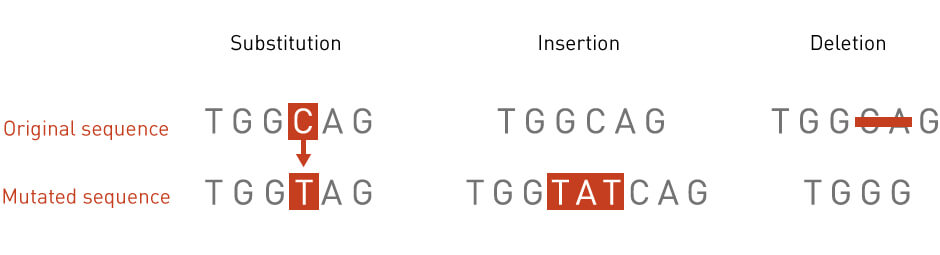
\includegraphics[width=4in]{images/background/muts.jpg}}
\caption{{\bf Some types of nucleotide mutations\cite{muts}} This shows the three most common variations. The SNP is on the left, then an insertion where a sequence is inserted, and the deletion where the opposite occurs}
\label{genfig2}
\end{figure}

Some diseases such as cystic fibrosis or sickle-cell anemia are inherited by a single gene that has mutated. These traits or diseases are called Mendelian because they follow a classical model of inheritance pattern which Mendel first described. Contrary to what may appear Mendelian diseases can happen with different variations in the same gene, with the same variation in the same gene, or with mutations in different genes that end up causing the same phenotype. All of these though are characterized by being caused by just one mutation. Predicting these types of diseases (or the risk of transmitting the disease to offspring) is easy to do, as just specific markers need to be analyzed and contrasted against common variants.\cite{nussbaum_mcinnes_willard_2016}
\newpage
In contrast, there are some diseases which are multifactorial and have a complex inheritance, such as Alzheimer's Disease, neuropsychiatric disorders or heart diseases. These diseases do not follow a Mendelian pattern of inheritance, and instead are thought to arise from complex interactions across different genes which modify the susceptibility to the given disease, and are then also affected by environmental factors as well as luck factors. Predicting these diseases is much more complicated and requires a broader set of factors to obtain meaningful results.\cite{nussbaum_mcinnes_willard_2016}

Knowledge about these mutations is only useful if the individual has a way of "reading" their DNA. This is done using Genome Sequencing, which allows analyzing sequences of base pairs to obtaining the existing DNA code in cells. Genome sequencing used to be prohibitively expensive 20 years ago but has since become much more affordable such that the general public can now use it (the first genome costed 2.7 billion USD , while it can now be obtained for 100-1000 USD). There are different types of Genome Sequencing: Whole-Genome Sequencing (WES)and Whole-Exome Sequencing (WES). The difference between the two is just a matter of scope, the second only analyzes the Exome, which is the 2\% of the genome containing exons (The protein-coding DNA). Generally WGS studies tend to have much more variants and information than WES, although the second ones are cheaper and thus could be used if the relationships are found in the exome. The specifics of the implementation of each won't be delved upon.



\subsection{Linkage (Dis)Equilibrium and Missing Heritability}
\label{missHerit}
One of the most important features of genetic analysis is Linkage. Linkage refers to the fact that due to natural selection, mutation, genetic drift and other biological and historical causes some alleles from different loci (and nearby in the genome) are associated in a non-random manner at a population level(That is, they are generally inherited together). Alleles are in Linkage Equilibrium when each Allele is independent of each other, conversely if they appear together with similar frequencies they are in Disequilibrium (LD), one such example analysis can be seen in figure \ref{genfig3}.\cite{nussbaum_mcinnes_willard_2016}

\begin{figure}[!ht]
\centerline{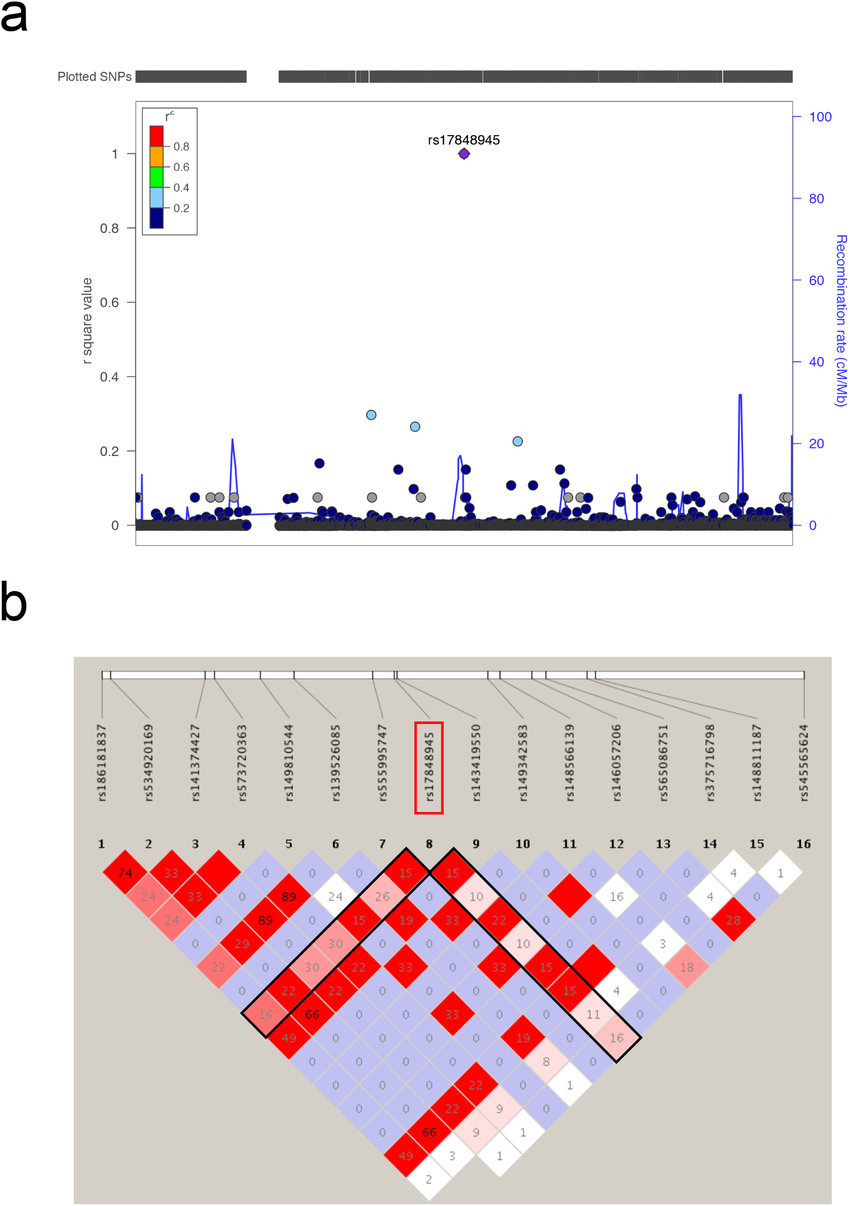
\includegraphics[width=4in,height=5in]{images/background/ld.jpg}}
\caption{{\bf Example of LD plots of marker rs17848945 \cite{ldfig}} Image a) gives the LD plot of the given SNP and the $R^2$ value of close SNPs. Image b) shows the LD block plot for further correlation analysis}
\label{genfig3}
\end{figure}

This has both positive and negative consequences. Positive, because if two alleles are closely linked, one can know the existence of one of those allele by proxy when knowing the other allele. This is useful for some tools such as Genome-Wide Association Studies and to do Linkage Analysis for detecting familiar diseases. Negative, because for predictive models this association between gene variants means that the system is fed inputs which are in correlation with each other and could generate results that are not valid or consistent, thus multiple those genes in linkage need to be processed in a way that they do not affect the data.\cite{nussbaum_mcinnes_willard_2016}

Another issue that complicates matters regarding genetic analysis is the Missing Heritability problem. One way to measure the genetic Heritability of a disease is with the use of Twin Studies, where genetic twins sharing the same genetic material are studied across different families to see if the disease or trait is genetic in nature or if it is environmental ( or a combination of both). Using these studies there are many multiple diseases which have been shown to have a medium-high genetic component, but when doing genetic studies the heritability that single SNPs or a mix of few foreground genes can explain is nowhere close to the estimated values of twin studies. Thus the genetic variations are unable to sufficiently explain the genetic factor estimated. One plausible theory is that the genetic influence is spread out across a multitude of background genes and interactions between them, instead of being an additive risk. Other theories discuss epigenetics, non-coding and exotic variants. As larger and more complete studies are done the highly polygenic hypothesis can be ascertained and validates.

\subsection{Genome-Wide Association Study}
\label{GWAS}
Genome-Wide Association Studies are one way to detect which gene variants are responsible or directly linked to a given disease by analyzing the whole genome in an statistical manner using a very large number of samples. They typically map the genome using millions of variants, taking advantage of the Linkage Disequilibrium phenomena. This is because if they map a variant which is in LD with the real variant related to the disease this correlation will then be visible in the variant mapped. In such a way, by using markers slightly spaced out they can reliably map the expected interaction of almost the entire genome with a fraction of the cost. And by obtaining samples from a very large group the statistical correlation between phenotype and the linked variants will appear (if it exists) thanks to the sample size.\cite{nussbaum_mcinnes_willard_2016}


One risk of GWAS though is population stratification, if subgroups exist within the data set the statistical results could find regional variants to be linked to the disease, thus care must be taken to ensure the population is the same for all samples. Another possible detail required is to limit the significance values strictly, as having such a big number of possible variants there is a high probability that by pure luck one out of the million SNPs will be close enough to be marked as significant when it is not. GWAS give an indication of the statistical relationship existing between a variant and a disease, with this a biochemical reason can be looked for in the candidate biomarkers to ensure the relationship is not purely statistical. Additionally, GWAS have shown proof than multiple common diseases are genetically complex in nature as well as highly polygenic.\cite{nussbaum_mcinnes_willard_2016}

\clearpage
\subsection{Polygenic Risk Scores}
\label{PRS}
As shown in previous subsections, the underlying hypothesis is that many complex diseases are characterized by being highly polygenic in nature, with each variant giving a very small adjustment in the risk, but when added up or combined together in a non-additive manner the genetic explanation starts to become much more robust and can explain a higher percentage of the missing heritability.

Extending this idea, Polygenic Risk Scores(PRS)\cite{pers} come as a natural extension to the problem. These are methods based on GWAS and other statistical samples that try to predict the risk a person has of developing a complex disease by analyzing these thousands of variants, instead of the few individual markers obtained from strict GWAS. Typically these PRS use some kind of regression analysis such as LASSO or ridge regression, and can even go as far as using the whole set of SNPs obtained from a GWAS as a reference. Some traditional PRS methods are Pruning+Thresholding and LDPred.

Thanks to larger datasets and more processing power PRS are being more and more widely used to predict the risk of developing complex diseases years before the first symptoms start and helping make environmental changes that could slow the development of the disease\cite{Torkamani2018}. One such example is the work done by the International Schizophrenia Consortium\cite{Consortium2009} . As shown in Figure \ref{prs1}, the PRS models which incorporates the highest number of SNPs gives a better explanation of the Variance that can be seen in the dataset. And further diseases with their respective variance values are also shown as a contrast.

\begin{figure}[!ht]
\centerline{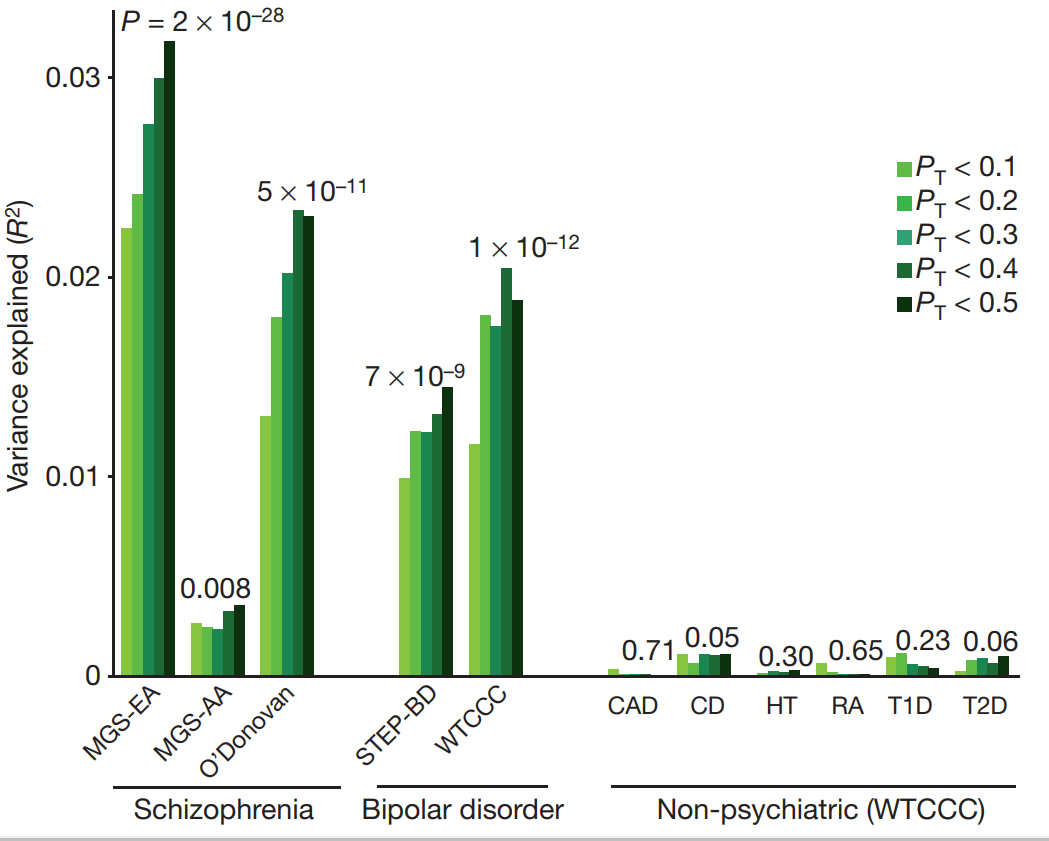
\includegraphics[width=3in]{images/background/prs.png}}
\caption{{\bf Calculated Polygenic component of Schizophrenia and Bipolar disorder, as well as non-psychiatric\cite{Consortium2009}} Calculated $R^2$ for Schizophrenia, Bipolar Disorder using different SNP thresholds. On the right are some common diseases. CAD, coronary artery disease; CD, Crohn’s disease; HT,
hypertension; RA, rheumatoid arthritis; T1D, type I diabetes; T2D, type II
diabetes.}
\label{prs1}
\end{figure}


\subsection{LDPred-funct}
LDPred-Funct by Dr. Marquez-Luna et al\cite{Marquez-Luna375337} is an extension of the LDPred algorithm first described by Vilhjhálmsson et al\cite{ldpreeed}. The LDPred algorithm increases the results obtained in PRS by modeling the Linkage Disequilibrium instead of pruning it (as the P+T method). This is done by estimating the posterior mean effect size of the given markers when fed LD information from an external cohort as well as prior information on those effect sizes. LDPred-funct then builds upon this system by incorporating into the model the trait-specific functional enrichments. Annotations are fit upon these functional priors and afterwards the LDPred-funct estimates the posterior mean effect size using these enrichments and annotations. A Cross-Validation method further improves the stability of the prediction as it does CV within samples, regularizing casual effect sizes.These improvements allow it to outperform the previous methods, as shown in Figure \ref{ldpred1} 

\begin{figure}[!ht]
\centerline{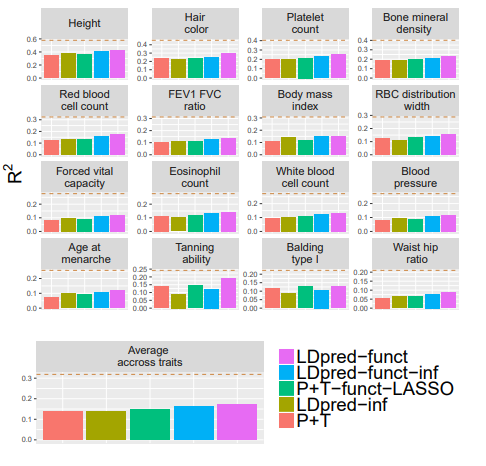
\includegraphics[width=3in,]{images/background/ldpred.png}}
\caption{{\bf Accuracy of PRS prediction methods on different UK BioBank phenotypes\cite{Marquez-Luna375337}} $R^2$ Results using 5 different polygenic methods using the UK BioBank dataset and evaluating 16 different phenotypes. The $R^2$ value is compared against the maximum calculated heritability value at the top of the graphs.}
\label{ldpred1}
\end{figure}
\clearpage
\section{Alzheimer Disease}

In this section the underlying theory behind Alzheimer Disease is explained as well as the progression that occurs from a person who is Cognitively Normal up to the point where Alzheimer Disease develops and Dementia is diagnosed. The multiple factors that are theorized to lead to the disease are also explained.

Alzheimer Disease is a neurodegenerative disease which targets an estimated 24 million people worldwide according to Ballard et al\cite{Ballard2011}. As he describes, the main markers in a person with Alzheimer Disease are formation of amyloid plaques and neurofibrillary tangles. Once a person begins to develop Alzheimer what occurs is that the $\beta$-Amyloid peptide 42 is generated from the amyloid precursor protein which then begins to store in the neuron and outside starts forming the plaques.These plaques then begin to form a cascade of sorts which slowly leads to cognitive impairment in the brain and finally to death. 

Mudher and  Lovestone\cite{Mudher2002} have proven one of the multiple hypothesis regarding the development of Alzheimer: A specific protein called $\beta$-Amyloid starts to develop in the brain, generating an excess formation of $\beta$-Amyloid plaques which in turn start blocking synapses between neurons in the brain and thus the breakdown of neurocognitive capabilities begins in a cascading manner. The Amyloid precursor protein suffers a fault in the onset of Alzheimer, which thus creates an Amyloid peptide A$\beta$1-42.
This peptide is the one that begins creating plaques and creates a cascade of other problems like tau aggregation and neuronal attrition. Figure \ref{gr1} shows the causes and development of plaques and the corresponding Dementia diagnosis.
\label{betaAmyloid}

\begin{figure}[!ht]
\centerline{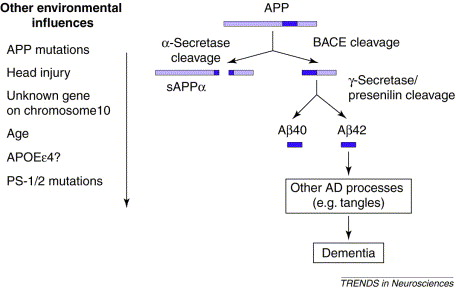
\includegraphics[width=4in]{images/background/gr1.jpg}}
\caption{{\bf Plaque formation and possible causes\cite{Mudher2002}} Development of Alzheimer's disease relating to the procedure via which the APP protein converts into Amyloid plaques that cause the disease. On the left are some possible environmental influences including the APOE $\epsilon4$ gene}
\label{gr1}
\end{figure}


Multiple other hypothesis exist for Alzheimer disease\cite{Scheltens2016} such as the tau hypothesis and retro-genesis. One of the main genetic component associated with the disease is the APOE $\epsilon4$ variant, if present, this variant reduces the breakdown of $\beta$-Amyloid in the body and thus an increase in plaques. The $\beta$-Amyloid hypothesis and its variants has shown in various tests a strong correlation which does indicate the right direction, but there are still multiple areas where research can grow to explain holes in the current formulation.

Meanwhile the Tau protein is the one which causes the aforementioned tangles, This protein is modified via the presence of a high concentration of $\beta$-Amyloid and results in the creation of some insoluble compounds that cause the neurons to cease functioning correctly. The Tau proteins also start forming sheets which are then transmitted to other parts of the brain and result in the spread of the disease. 
\newpage
Scheltens gives \cite{Scheltens2016} some other Biomarkers besides Tau protein concentration and $\beta$-Amyloid plaques to detect Alzheimer. Some of the are A$\beta$ oligomers, some synaptic proteins such as neurograning and SNAP25. These are found in the cerebrospinal fluid and as such are not so easy and cheap to detect. Thus he also mentions some blood biomarkers, one example being CNS proteins, but this area is still lacking.

In the same paper \cite{Scheltens2016} it is shown that the lifestyle and demographics of the patients can affect the risk factors of developing Alzheimer. Clearly the main factor is age, but Diabetes, Obesity, lack of mental stimuli and depression can increase this risk by up to 30 percent.

Ballard demonstrates that not only biomarkers play an important role, but that the genetic code has a high impact on the formation of Alzheimer, as some genes promote the formation of Tau sheets via generation of compounds that phosphorilyze Tau proteins, others increase the burden of  $\beta$-Amyloid particles and some others increase the amount of Amyloid precursor protein available. These genes can increase the risk of Alzheimer by up to 70 percent. Scheltens also agrees on this point and does show the same results regarding the genetic factor.

The Early Onset disease follows a very Mendelian inheritance pattern, with mutations in the APP, PSEN1 and PSEN2 related genes causing the disease almost certainly. But the genetic component of Late-Onset Alzheimer is a much more complex one. As seen before it is one of those multifactorial, complex and polygenic diseases that are most complex to determine. The APOE $\epsilon4$ variant is definitely the main genetic factor to consider as a risk indicator, but multiple other genes have been shown to have correlation with the disease as CLU, ABCA7, BIN1 and others which can be seen in Figure \ref{genAD}. Most of these genes have been shown to have a biochemical relationship with the  $\beta$-Amyloid production process, and as such they are not only statistically significant. There are variants in multiple pathways each of which gives a very small risk increase but can overall have a large impact on the risk factor which is then further amplified by the environmental factors. Furthermore, some mutations have compounding effects, one SNP in PSEN1 with patients who also carry the APOE $\epsilon4$ mutation have a much higher risk of developing the disease than those that don't have both mutations. Thus, approaches that use a multitude of genes with nonlinear combinations might perform better than single-SNP diagnosis.\cite{KARCH201543}

\begin{figure}[!ht]
\centerline{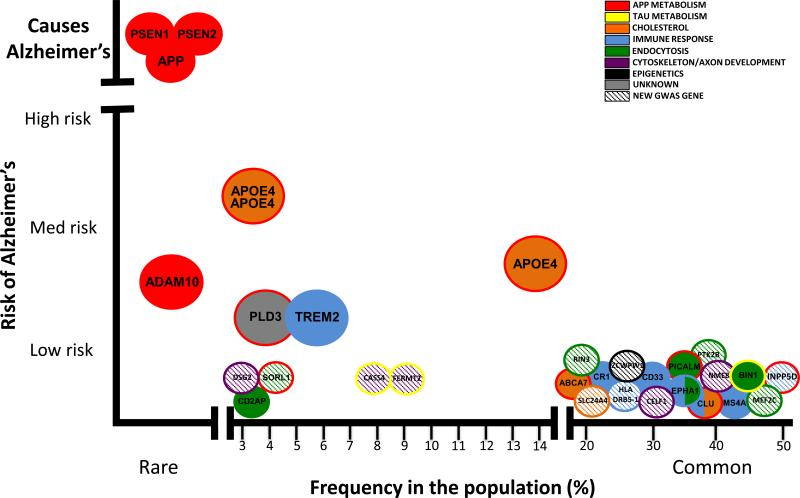
\includegraphics[width=4in]{images/background/genad.jpg}}
\caption{{\bf Genetic variants that contribute to Alzheimer's Disease\cite{KARCH201543}} These are some of the genes as well as the biological functions they play that increase the risk of developing Alzheimer's Disease}
\label{genAD}
\end{figure}


As shown by the National Institute on Aging\cite{McKhann2011}, the clinical diagnostic of Alzheimer's disease (and by proxy, the stages leading to it) is quite complex. The one way to know without a doubt if a patient has Alzheimer's Disease is by doing a postmortem autopsy and finding the amyloid plaques that impair the brain, this is useful for research but clinically speaking it is pointless. Other diagnosis while the patient is alive consider the use of cognitive tests to test the patient's ability to memorize or perform complex tasks. Bio-marker concentrations seen before can also be used to diagnose the state of Alzheimer's disease. Furthermore this problem is complicated as someone who might not have Alzheimer's (Or even any type of Cognitive Impairment) could develop the disease after some years, with very different rates of development across individuals. Some patients go from Cognitively Normal to Alzheimer's almost directly, some never make the jump from Mild Cognitive Impairment to AD, and some others can have a regression (Mostly due to clinical or test errors) Thus, this makes it so that working with Alzheimer's databases for diagnosis something quite complex as there is uncertainty regarding whether the sample being analyzed is truly a control or if it is just a case lying dormant as a control for the point in time taken.

Due to some of the complications present in the clinical diagnosis there is also interest in detecting the presence of Alzheimer's Disease or possible early signs of the development by the use of longitudinal data using Biomarkers or Magnetic Resonance Imaging as an aid to help the detection process. These models could take the data of a given patient and tell the doctor through an analysis why the system believes the patient to have the early signs of Alzheimer's which are consistent with the results found in other patients. By detecting it in an early stage the patient can start taking decisions with respect to the disease and analyze prospective treatments before it is too late.

The gold standard though, would be the prediction of Alzheimer's disease decades before it's onset, or at least a risk indicator which could give the patient the knowledge required to make environmental changes that might slow down the progression of the disease or the use of medicines designed to have an impact at the earliest stages of the (as is the case with most drugs being analyzed that stop the amyloid plaques from developing). 
\clearpage


\section{Machine Learning}

Machine learning is a form of data analysis that has existed for decades but has recently seen a big increase in terms of popularity and performance thanks to the increase in available data as well as processing power. Through the use of a plethora of algorithms and models a computer can be trained to find specific and desired patterns in a sea of data to accomplish reliably a given task such as detecting a disease. Machine learning is commonly split in three categories: Supervised Learning, Unsupervised Learning and Reinforcement Learning. The first category is the one of interest in this thesis, where the algorithms are given sets of labeled data from which to learn and adjust across multiple iterations depending on the correctness of the prediction. Then the resulting model is extrapolated to a validation or testing dataset to ensure the performance is valid.

This section gives the background information of the machine learning methods used in this thesis. It begins with describing Support Vector Machines(SVM), and Random Forest(RF). Afterwards an in-depth description of Neural Networks and Deep learning is given with the multiple hyper-parameters that can be tuned and adjusted. Then it gives an analysis of the FRESA.CAD benchmark as well as the component methods that are used by it.

\subsection{Support Vector Machines}
\label{RF}
Support Vector Machines are Machine Learning models first proposed by Boser, Guyon and Vapnik\cite{Boser:1992:TAO:130385.130401}. SVMs try to optimize the problem by finding a hyper-plane in the feature space being given as input where it can distinctly classify the two different classes. This is obtained by maximizing the margin between the chosen hyper-plane and the so-called Support Vectors. Support Vectors are the sample points close to a given hyper-plane that would then give the location and orientation of the classifier, and which are iterated and selected to obtain different points. Thus, by maximizing the margin finding a boundary in a higher-dimensional space where it can separate the classes apart. Figure \ref{svm1} shows an example of how the SVM Hyper-plane is selected and the role the Support Vectors play in maximizing the margin, as shown the Support Vectors chosen tend to be those close between the classes. This is further expanded upon by using something called the kernel trick, where a transformation is done to the input where it is extended into a higher-dimensional space and depending on the chosen kernel gives a Non-linear representation of the data where the hyper-plane separation can be done. This then allows a more robust and complete transformation allowing non-linear classification. 

\begin{figure}[!ht]
	\centerline{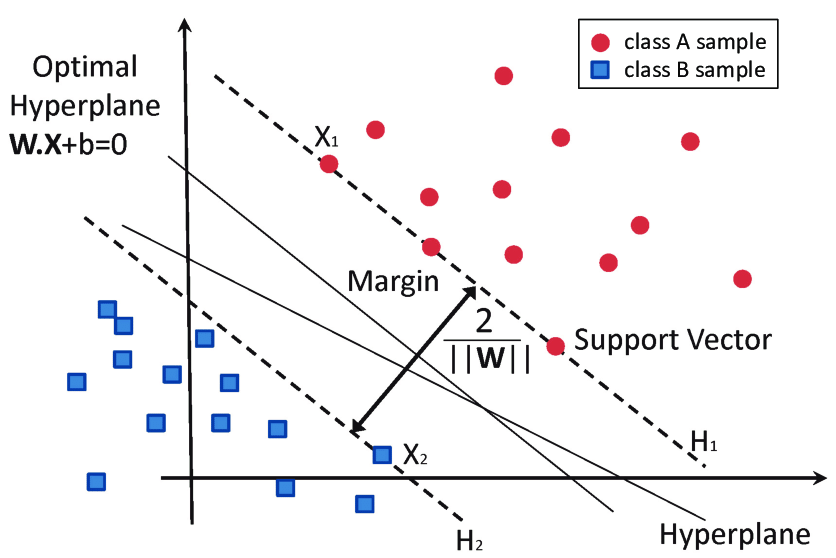
\includegraphics[width=5in]{images/background/svm.png}}
	\caption{{\bf Support Vector Machine Hyper-plane classification \cite{svm1}}
		An example of the hyper-plane classification being done by a SVM. The data samples from different classes nearby are chosen as Support Vectors and a hyper-plane is chosen which maximizes the margin between classes.} 
	\label{svm1}
\end{figure}

\subsection{Random Forest}

Randoms Forest is another Machine Learning method which can be used for the classification task. It was first presented by Ho\cite{598994} and also gives very robust and precise results. It works by doing an ensemble of a multitude of Decision Trees, from which it then takes the mode of the results given by all of trees. Each tree is given a random subset of features from the total input features and then builds the tree using the best features out of that subset.  Thanks to using different decision Trees, each of which uses a different random subset of features for the classification task the random forest helps avoid over-fitting and obtains results that are more accurate and stable on the validation results as a Wisdom of the Crowd model. Figure \ref{rf1} gives an example of the structure a Random Forest follows.

\begin{figure}[!ht]
	\centerline{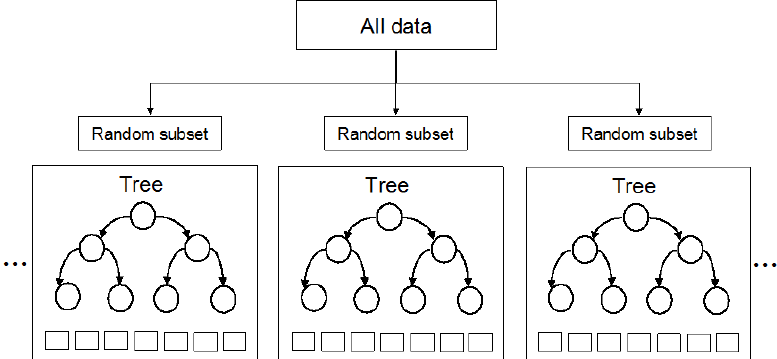
\includegraphics[width=5in]{images/background/rf.png}}
	\caption{{\bf Random Forest Structure\cite{rf}}
		The diagram shows an example of the structure a Random Forest follows, with different trees each using a subset of random features.} 
	\label{rf1}
\end{figure}

\clearpage
\subsection{Neural Networks and Deep Neural Networks}
\label{DNNs}
Artificial Neural Networks (ANN) are yet another Machine Learning tool for supervised learning. The basis of an ANN is the perceptron, dating back to 1958 and first described by Rosenblatt\cite{Rosenblatt58theperceptron:}. This is a mathematical model based on the neurons of the brain, where there are multiple inputs each multiplied by given weights that enter the perceptron, and in some cases applying an operation (Activation Function), which gives an output consisting of a linear combination of these features. Figure \ref{percep1} gives a visual description of the model a perceptron follows. A simple perceptron thus can be used as a classifier, where it will be able to do linear classification and as such is limited. 

\begin{figure}[!ht]
	\centerline{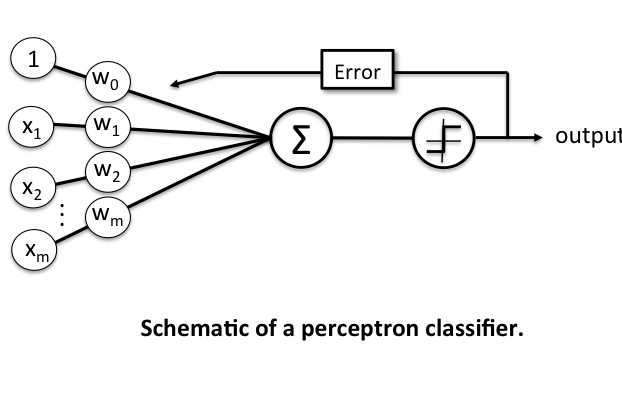
\includegraphics[width=5in]{images/background/perceptron.png}}
	\caption{{\bf Perceptron Model\cite{percep}}
		The model describes a simple single-layer perceptron with the inputs on the left, followed by the weights by which to multiply them, the sum done in them and finally the activation function that leads to the output. The feedback error to guide the learning process is also shown.} 
	\label{percep1}
\end{figure}
When using multiple layers of these perceptrons the performance and prediction capabilities of the resulting network is greatly enhanced. These multi-layer perceptrons (MLP) are thus Artificial Neural Networks, an homage to the biological source of inspiration (Even if the similarity is no longer there). Artificial Neural Networks typically consist of an input layer, which is then connected to an intermediate (or more) hidden layer (named as such as it is not directly observable), the hidden layer then connects to the output layer and gives a result. Then this output is compared to the actual label and the network is adjusted accordingly. A series of iterations are run with the available samples and across multiple repetitions called epochs to successively train the network.

Two methods are crucial to the inner working of the ANNs: Forward-propagation and Backpropagation. The first is the one responsible to propagate the input data across the successive hidden layers until it reaches the output layer. It does this by the previously described method in the perceptron multiple times over both in terms of layers and in terms of the respective neurons per layer. Backpropagation takes the error value obtained when comparing the obtained output with the real output, and obtaining the error derivatives for the output layer, then sending that backwards towards the hidden layers and all the way back. The derivatives are then used to calculate the adjusted values of the weights to correct this error and the model is updated. By using the gradient respective to each weight each of them is adjusted towards the correct direction for a precise result. The weight update incorporates an important value: the Learning rate, this is a hyper-parameter than will control how much the weights will be update iteration, to ensure the learning is not done too slowly, but that it doesn't overshoot either. Figure \ref{dnn1} gives an example of the architecture of a neural Network, while also describing the forward-propagation and the backpropagation methods in a visual manner coupled with the respective mathematical formulation.

\begin{figure}[!ht]
	\centerline{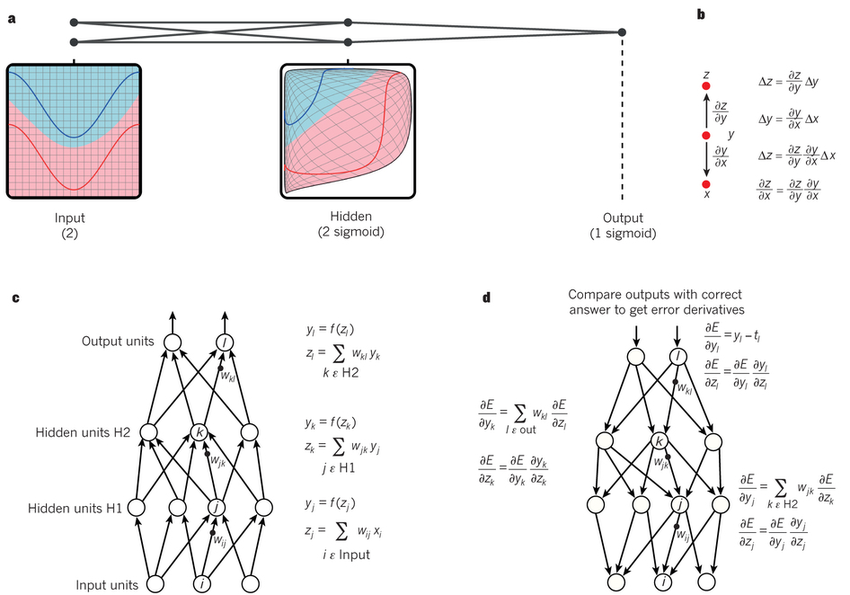
\includegraphics[width=5in]{images/background/deepnet.png}}
	\caption{{\bf Neural Networks, Forward-propagation and Backpropagation\cite{LeCun2015}} a) shows how MLP can make an input linearly separable by transforming the input space. b) shows the backpropagation error equation in terms of derivatives. c) gives the forward-propagation equations in a sample DNN, while d) describes the backpropagation } 
	\label{dnn1}
\end{figure}

According to Yann LeCun\cite{LeCun2015} Deep Learning is a method which allows to learn the representation models of data using multiple processing layers. Thanks to how the model is distributed in multiple layers and each layer affects the next ones the higher-order layers begin to learn more abstract structures in the data which are not detected in the first stages and can thus give a better solution to a given problem. Furthermore the different layers can use back propagation to give feedback to lower layers on which weights to adjust from the neural links and thus improve the representations all across the network. 

Schmidhuber defines\cite{Schmidhuber2015} the description of what makes a neural network deep: it has a considerable depth of its credit assignment paths which tends to be larger than 3. This depth and the choice of how many hidden layers as well as how many neurons will be present in each layer are the most important parameters to modify when creating a deep neural network and can have quite varying degrees of success. 

An activation function is a crucial component of a neural network node. These are the functions that describe how the neural network will interpret the sum of its inputs and thus obtain one output. Multiple activation functions are used and the results of the network can vary greatly depending on them. Some examples of activation functions are: Logistic, Rectified Linear Unit(ReLU) and its variations, Binary Step, TanH, Softplus, Gaussian, etc. The most commonly used activation function is the ReLU, first described by Nair and Hinton\cite{Nair:2010:RLU:3104322.3104425}. This activation function has multiple benefits arising from a more biologically-inspired perspective:

\begin{itemize}
	\item It has no output values other than 0 when having a negative inputs, consistent with biological neurons. 
	\item It propagates the gradient efficiently.
	\item It has a sparse activation, which allows the model to learn more efficiently in a distributed manner. 
	\item it is scale-invariant with respect to the input.
	\item It is computationally efficient thanks to using only addition and multiplication.
\end{itemize}
\newpage
The equation for the ReLu is quite simple and is as follows:

\begin{center}
	$f(x)= max(0,x)$
\end{center}

One of the main problems with Neural Networks which also has a greater impact for Deep Networks is the vanishing gradient problem, as the gradient is sent forward and backwards using the gradient of the chosen error function the gradient starts to get smaller and smaller due to applying the chain rule with functions from -1 to 1.  The ReLU unit can reduce the vanishing gradient problem thanks to how it goes from the desired value to 0 directly when it detects a 0 or lower in its input

The selection of a Loss function for the Neural network is another factor which can be modified to obtain different results. The Loss function indicates how the resulting output is valued and thus how back propagation will be calculated and sent back throughout the whole network. Thus it encodes the cost or value of giving a specific output depending on the real world solution desired. Back propagation calculates the gradient of this loss function and then updates every neuron through it. Multiple loss functions can be used and this will modify the way the neurons will learn and the weights will be modified, thus care must be taken. There are multiple cost functions, some of the most common ones are Mean Squared Error, Root Mean Squared Error, Soft max. For classification problems one of the most widely used is the Cross-Entropy Loss which is described by the following formula given 2 possible classes (where y is the real label and p the predicted label):

\begin{center}
	$-(ylog(p)+(1-y)log(1-p)$
\end{center}

This loss function will try to minimize the distance between the predicted probability distribution and the real probability distribution of the classes. To correctly use Cross-Entropy the output of the final layer must be a probability and as such the final output layer must be a Sigmoid activation function or similar. Additionally, Cross-Entropy improves the Sigmoid activation by avoiding getting the neuron saturated and will not slow down the learning process.

The final choice of crucial hyper-parameter to tune in the Deep Learning Networks is the Optimizer. These are the algorithms responsible to minimize the desired loss function by adjusting the weights, bias and in some cases the learning rate. Typically these use the Gradient of the function as described before to calculate the adjustments (But some can use the Hessian). Some of the classical optimization algorithms for Neural Networks are Gradient Descent with its variants such as Batch and Stochastic Gradient Descent, Momentum Descent, Rmsprop, Adagrad among others. 

But typically one optimization algorithm is used almost always above the others due to its performance in multiple tasks: Adam. Adam is an optimization algorithm developed by Kingma and Ba\cite{DBLP:journals/corr/KingmaB14} which extends the Stochastic Gradient Descent algorithm. Its name stands for Adaptive Moment Estimation, and it does it by adapting the learning rate for each parameter based on estimates of the mean (first moment) and the variance (second moment) of the calculated gradients. Some of the benefits of this algorithm are the following:

\begin{itemize}
	\item Efficient to calculate and cheap to store.
	\item Easy to scale.
	\item Few tuning parameters to adjust.
	\item Works correctly with sparse or noisy datasets.
\end{itemize}


One of the main problems of DNNs (and in Machine Learning in general) is overfitting, where the learned model trains too much on the training set, memorizing it perfectly but while doing this it loses the ability to generalize and performs worse in samples that have not been seen before (such as the validation dataset). This is a deal-breaker for most applications and as such multiple methods have been traditionally used to process the data, reducing the over-fitting and increasing the performance on the validation dataset. Dropout, Normalization and Regularization are the main tools employed to achieve this and most DNN currently use a mixture of them.

Dropout as a method was first proposed by Srivastava, Hintont et al\cite{JMLR:v15:srivastava14a} in 2014 as  a powerful yet simple way to minimize overfitting and thus making the algorithms more precise in the validation and training stage to be able to generalize without specializing too much into the training set. Dropout as a concept is very simple. Neurons are randomly deactivated with a given probability all across the network in the training phase, which means they don’t affect the next layers and they do not learn (Those weights are effectively frozen). This allows to sample a thinned out version of the network, and each of the iterations has a different thinned network, all of these get combined. This can be seen as a way of putting together many different models to get a prediction which in average performs better. Also, the way this is done enables the training to be spread around the different neurons and weights instead of being specifically trained just for one case. Dropout has been so efficient at preventing overfitting that it is the most widely used 


L2 regularization has been used by many researchers, such as Andrew Ng which was one of the first to apply it for Neural Networks\cite{Ng:2004:FSL:1015330.1015435}. Regularization is used to penalize more complex models (which are more prone to overfit the data), by minimizing both the Loss function and the complexity of the model. The L2 equation is the sum of the squares of all weights at a given layer, and it is expected to be as low as possible. L2 regularization will then penalize harshly those weights that have a strong impact with respect to the other weights and will try to keep them close to zero, thus reducing the complexity of the model and regulating the weights across the layer. This will most certainly decrease the overfitting while maintaining good performance.

Batch Normalization is a method created by Ioffe and Szegedy\cite{Ioffe2015BatchNA}, used in tandem with Batch updating which normalizes the activations across the batch. It analyzes the mean and variance present for every feature in the training batch and then normalizes the inputs by subtracting the mean and dividing by the standard deviation, then scales and shifts the normalized activations. Batch normalization helps control the magnitude of the activations and as such smooths the loss function (as well as damping oscillations) which makes the corresponding optimization process work in a more efficient way. 


\subsection{FRESA.CAD Benchmark}
\label{fresaCAD}
FRESA.CAD is a benchmarking package in R ( openly available in the CRAN) created by Dr. Taméz Peña\cite{fresa}, which evaluates the repeated holdout cross-validation (RHCV) of binary classification algorithms or feature selection (FS) algorithms, and returns a set of all the test results. Figure \ref{fresafig1} shows the RHCV implemented in FRESA.CAD. The repeated test results are then combined into a single prediction per sample, returning the classifier performance for further analysis. The summary performance statistics also include the 95\% confidence intervals to check statistical confidence. The implemented RHCV also returns the selected features at each train instance. 

\begin{figure}[!ht]
	\centerline{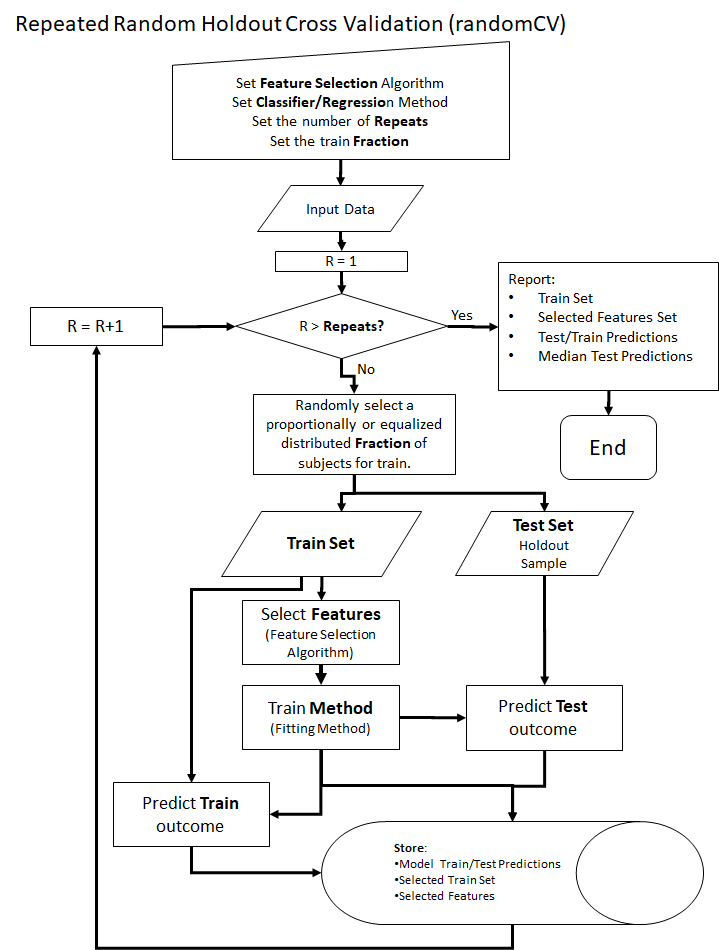
\includegraphics[width=4in]{images/background/fresaRCV.png}}
	\caption{{\bf Repeated Holdout Cross-Validation with FRESA.CAD\cite{fresa}}
		The flow diagram depicts the RHCV procedure implemented in the FRESA.CAD benchmark used to split the input dataset for training and validation} 
	\label{fresafig1}
\end{figure}


All of these factors make it so that there can exist a comparison between different classifiers and feature selection algorithms under the same environment, ensuring there is no variation due to train/test sets or filtering algorithms. The benchmark takes a dataset and runs a set of predetermined classifiers and feature selection algorithms. Furthermore, FRESA.CAD allows the simple exploration and comparison of the selected features of each filter method to identify features that could be of use. Figure \ref{fresafig2} shows the workflow of the benchmark procedure, which by default uses Bootstrap Stage-Wise Model Selection (BSWiMS) as the data-classifier method.

\begin{figure}[!ht]
	\centerline{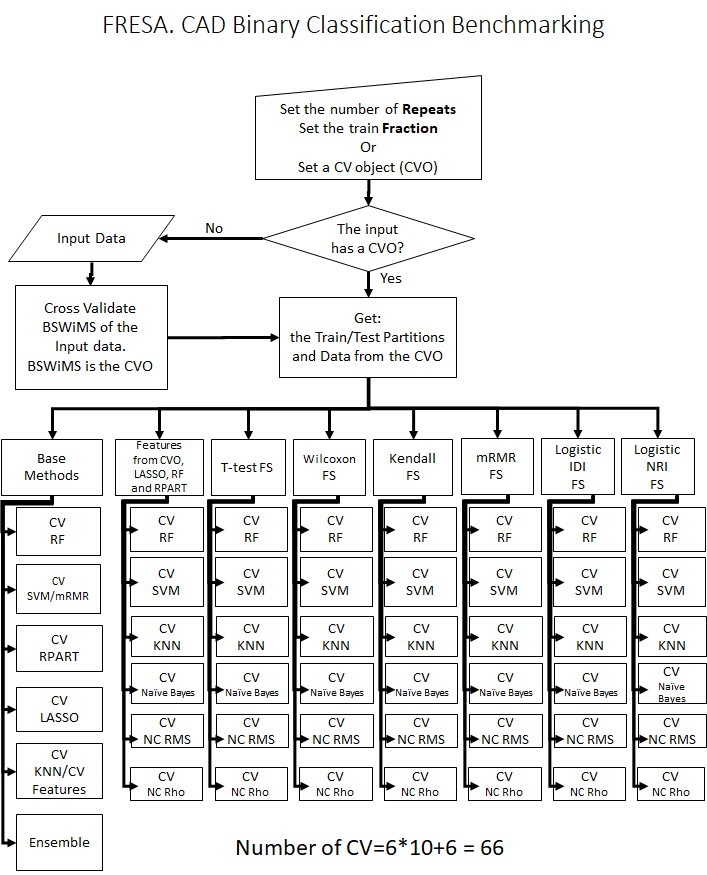
\includegraphics[width=4in]{images/background/FresaBinBen.png}}
	\caption{{\bf FRESA.CAD Benchmark procedure\cite{fresa}} The flow diagram depicts the Benchmarking procedure across the different models and filters for comparison in each Cross-Validation iteration}
	\label{fresafig2}
\end{figure}

The results of the Cross Validation instances executed by the FRESA.CAD Binary Benchmark can be compared with the performance statistics and they are then ranked by comparing each CV instance 95\%CI. The ranking method accumulates a positive score each time the lower CI of a performance metric is superior to the mean of the other methods and loses a point each time the mean is inferior to the top 95\%CI of the other methods. Additionally, the package returns the accuracy, precision, sensitivity, the balanced error rate and the ROC area under the curve with their corresponding 95\% confidence intervals (95\%CI). The plotting functions included with the package make the visualization and comparison much easier and useful.

\clearpage

\section{Previous Work}

The first segment will describe work done with Deep Learning using genetic data with different diseases. Another topic described will be the detection of Alzheimer disease via Machine Learning methods to give an overview of what has been done and has worked to detect it directly based on observations, Finally, the state-of-the-art as well as investigations previously taken in the area of Alzheimer Disease prediction are described.
 
\subsection{Genetic Prediction with Deep Learning}

Deep Learning has recently arisen as a tool used for Genomics analysis to understand the vast amount of data available in all the different pathways of the chromosome. Thanks to the processing power of Deep Learning the vast number of links and relationship among genotypes, phenotypes, proteins, regulation and others could be understood with more precision. Deep Learning must be implemented with care and following appropriate guidelines to ensure the models do not overfit or the results given are not biologically consistent.\cite{Zou2019}

One such use of Deep Learning is by Sundaram et al\cite{Sundaram2018}. They describe a method via which they can predict the clinical impact of human mutations, selecting those variants that actually do have an impact in terms of diseases instead of those variants that are harmless. They start from the idea that those mutations that are present across multiple other species will also be benign for humans, thus reducing greatly the number of SNPs to look for disease correlation. They train a deep neural network on the primate and human datasets which learns to predict the pathogenicity a mutation will have based on the change in amino-acid sequence . This is supported by two other networks that predict the secondary structure and the solvent accessibility of a given amino acid sequence. Figure \ref{predHum1} shows the general structure of the algorithm used as well as the results obtained, of note is how the Deep Network correctly assumes that mutations in the functional domains give a higher risk score. This method then identifies rare diseases and the respective genes that cause them with 88\% accuracy, while also giving 14 possible new candidate genes that are related to intellectual disabilities. Thus showing the value of Deep Learning applied to a genomics problem.

\begin{figure}[!ht]
\centerline{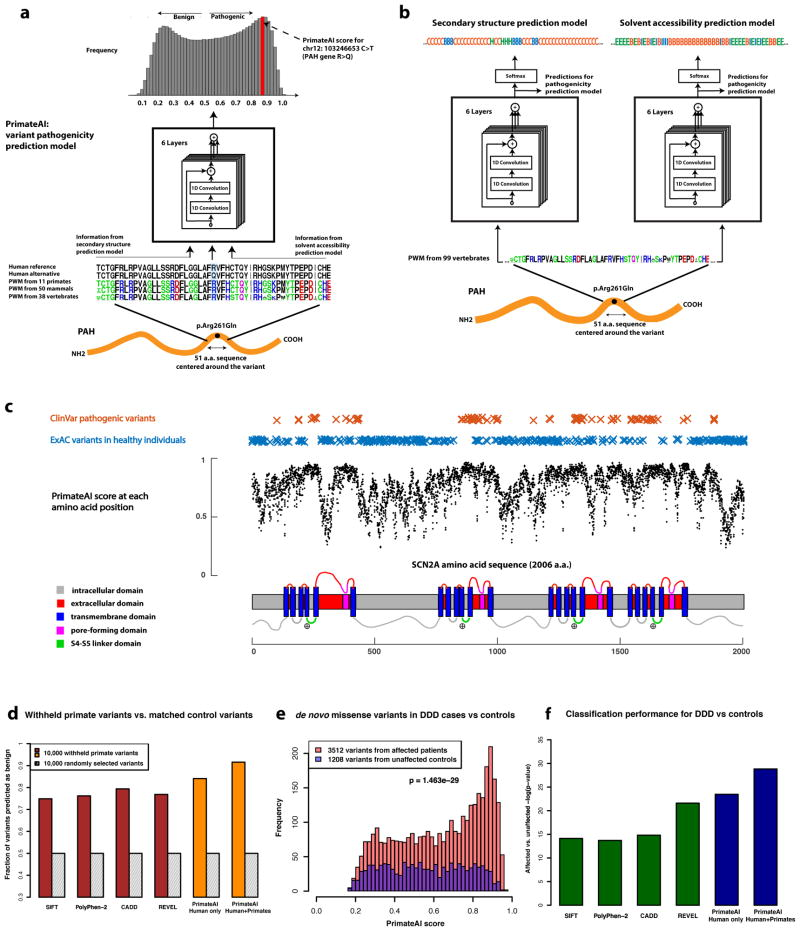
\includegraphics[width=5in]{images/background/predHum.jpg}}
\caption{{\bf Deep learning Architecture and results\cite{Sundaram2018}} Image a) describes the deep network architecture to predict pathogenicity depending on the given Amino Acid sequence variant, the reference and the support network results. Image b) describes the structure of the support deep networks for predicting the secondary structure and the solvent accesibility. Image c) shows the predicted pathogenicity given to mutations at specific points, as well as the reported ClinVar pathogenicity.  Image d) e) and f) give the results obtain with respect to withheld variants, missense variants and classification performance}
\label{predHum1}
\end{figure}
\newpage
\clearpage
Another approach using Deep learning is from Zhou and Troyanskaya\cite{Zhou2017}. They designed a method by which they can predict the effect that de-novo noncoding variants can have. Traditionally, the noncoding variants are ignored with respect to coding SNPs, but using the Deep-Convolutional-Based DeepSEA framework the model can use the data from noncoding variants to predict the impact they will have. The structure followed can be seen in \ref{predeff1}.

\begin{figure}[!ht]
\centerline{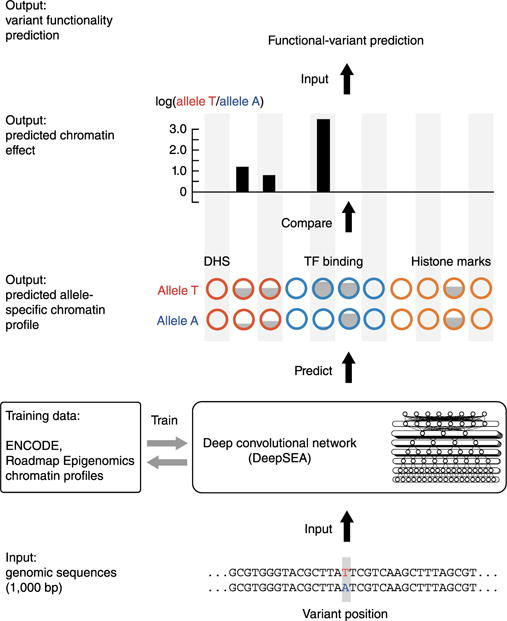
\includegraphics[width=4in]{images/background/predeff.jpg}}
\caption{{\bf Overview of the prediction Architecture\cite{Zhou2017}} The diagram describes the schematic overview of the system. The Deep network receives the sequence at the genetic variant, from which it predicts chromatin profiles contrasts it between the reference and the variant and thus obtains a prediction on the functional effects.}
\label{predeff1}
\end{figure}
\newpage
\subsection{Alzheimer Disease Detection}

Machine Learning approaches for Alzheimer detection have seen a surge in interest in the latest decade. Mishra et al introduce\cite{Mishra2017} a method via which they use the AV-1451 PET Imaging to obtain readings of tau particles which they then parse using unsupervised learning the results of the imaging to find the most informative segments of the brain. Orrú et al show\cite{Orru2012} a Support Vector Machine approach to identify and detect useful biomarkers for prediction and detection of Alzheimer Disease as well as other mental diseases Klöppel et al\cite{Kloppel2008} also use the Support Vector Machine model to classify Alzheimer Disease from a group of patients using MRI scans and achieving up to $96\%$ accuracy.


Neural Networks are an ideal approach for Alzheimer Detection as the causes of the disease are still not very well understood and a myriad of factors can increase the chances of someone developing it, with most of them working in tandem or affecting each other. Multiple biomarkers, genetic information, demographics and even lifestyle habits can be used as input features together. A neural network can take all of these features, understanding and estimating the inherent underlying nonlinear models. This allows it to construct, thanks to its intrinsic learning of representation models, a good estimator of the way these features interact with each other and signify the onset of Alzheimer, thus detecting it.

One of the approaches for Alzheimer Detection is from Sankari\cite{SANKARI2011165} where they use a probabilistic Neural Network to classify between Cognitive Normal and Alzheimer in a control group. The model uses features obtained from coherence studies from and Electroencephalogram. Using the extracted features from the studies they trained a the probabilistic neural network, containing 4 layers: Input, Pattern,Sum, and Output. By representing patterns using Parzen windows and a Gaussian distribution as groundwork the team was able to obtain up to $100\%$ accuracy in the classification via conventional coherence.

Suk, Lee and Shen\cite{Suk2014} propose a feature representation model for Alzheimer Disease detection which can be used in deep learning. They start with MRI and PET imaging information which they then convert into a high-level latent representation model which contains the shared features rich with information. They utilize a Deep Boltzmann Machine to obtain these feature representations, as it can be seen in Figure \ref{gr2}. With this method they managed to obtain up to $95\%$ accuracy with the ADNI data set in predicting whether a patient would have Alzheimer or not using only the imaging information transformed. The deep networks were capable of extracting the high level patterns and models existing between the data.

\begin{figure}[th]
\centerline{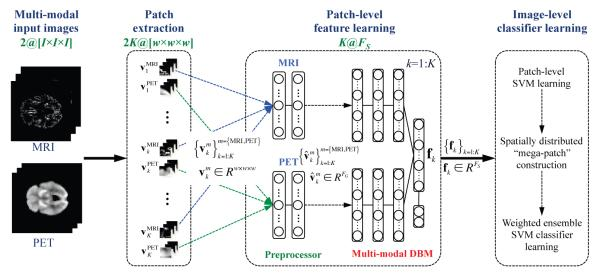
\includegraphics[width=5in,height=3in]{images/background/gr2.jpg}}
\caption{{\bf Suk et al proposed method for deep learning\cite{Suk2014}}{ Method via which they create a feature representation model using deep learning by extracting patches from MRI and PET images which they process and then feed into a Deep Boltzmann Machine, the outputs of which are then classified using a SVM. }}
\label{gr2}
\end{figure}

Liu et al describe\cite{Liu2015} a multimodal approach which tries to solve the problem in efficiency of biomarker representation by using a deep learning architecture. They use the ADNI data set and from those obtained the MRI, demographics, PET data and then assembled them using a Multi-Modal deep network which obtains the fused data representation, this structure can be seen in Figure \ref{gr3}. Then they use this resulting data representation in the network to finally obtain the resulting diagnostic of the disease. The results obtained using this method obtained the best results out of comparisons with Support Vector Machines and gave the best results when they were fused with the most amount of features.

\begin{figure}[th]
\centerline{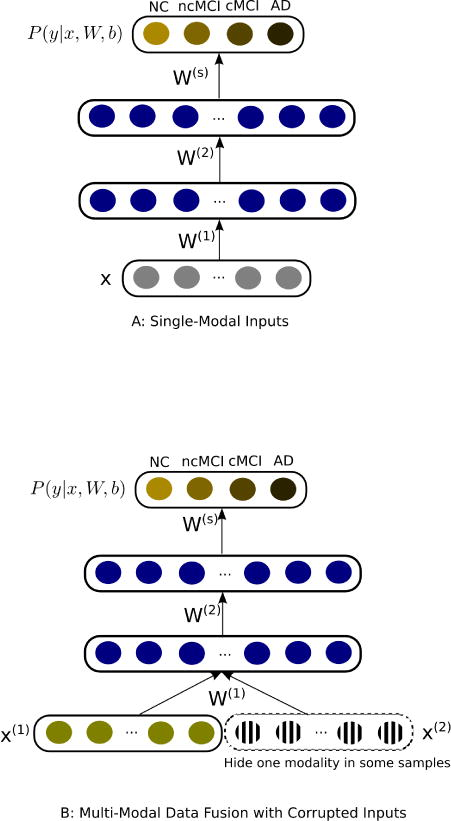
\includegraphics{images/background/gr3.jpg}}
\caption{{\bf Architectures from Liu et al\cite{Liu2015}}{ The architecture used to train Deep Learning architectures, first being single-modal and afterwards with the better multi-modal structure to predict the 4 classes.}}
\label{gr3}
\end{figure}

By utilizing their system they were able to obtain a feature representation in one go while requiring less information and achieving a performance gain.
\newpage
\subsection{Alzheimer Prediction}

The other main component to tackle the Alzheimer Disease problem is prediction. Many proposed medications and treatments are counting on treating the patients before Alzheimer is diagnosed as it is usually too late to have an effect. Thus models that can accurately predict the future development of Alzheimer disease are quite useful for preventive treatments.

Rowe et al created\cite{Rowe2013} an algorithm that could analyze $\beta$-Amyloid imaging, memory performance, hippocampal atrophy and the APOE $\epsilon4$ gene to predict Alzheimer disease after 3 years of the study. By using multivariate analysis they were able to find strong correlations between $\beta$-Amyloid plaques, decrease in Episodic Memory tests and the development of Alzheimer in a couple of years.They were also able to identify that those individuals with high impairment in the EM test and positive $\beta$-Amyloid plaques will progress to Alzheimer. They conclude that $\beta$-Amyloid imaging is a strong predictor of Alzheimer disease.

Mathotaarachchi et al developed\cite{Mathotaarachchi2017a}an algorithm which can assess and predict the development of Alzheimer Disease in a period of two years. They obtain information from the ADNI database using the PET scan regarding the concentration of amyloid particles and then use this information in a probabilistic approach to train a Random Forest-based algorithm called RUSFR (Random under Sampled Forest With this they can then generate predictions in this 2 year interval. Using this method they predicted the results and obtained an area under the ROC curve of 0.906 which performed better than a SVM and L2 Regression. This shows the potential use of only PET imaging data for predicting Alzheimer Disease before its onset.

Long, Chen, Jiang and Zhang describe\cite{Long2017} a method where they utilize MRI imaging to obtain information regarding deformation of the areas of the brain. They then use this data to diagnose and predict the onset of Alzheimer disease. They start by obtaining the distance between subject, and then using a distance matrix and a multi-dimensional scaling algorithm to embed data. This data is then used to classify it via a Support Vector Machine to obtain the resulting diagnosis of the patient. The resulting method correctly differentiated cognitively normal and Mild Cognitive impairment in $96\%$ of the cases and obtained an area under the ROC curve of 0.98 for some specific areas of the brain.

	% % ********************** PART 2
		% ***************************************
% ***************************************
\chapter{Materials and methods} \label{materials_and_methods}
% ***************************************
% ***************************************
In this section the actual characteristics and details of the proposed solution will be described, as well as the metrics used for validating the obtained results. The Data set being used will be documented in detail as well as the further changes and selections done to it. The Tools and Software that are employed in method are also discussed. A thorough description of the Quality Control Pipeline being used to process the genetic data is given. Next, the Neural Network architecture being used is described, considering the different Hyper-parameters and structure selected. Afterwards, the Simulation and Data Augmentation methodologies are described in detail to give the specifics of both cases. A brief description of the models used with the FRESA.CAD benchmark as well as the parameters set follows the Simulation and Data Augmentation segment.Then, the changes and settings for the LDPred-funct experiment are shown. Finally, the Validation Methodology as well as the Metrics used to evaluate performance are described.

\section{Data set}
 
The selection of an appropriate data set for training and testing is crucial as the machine learning algorithm will be as good as the information provided to it. A skewed data set will give skewed results and an empty data set will not be able to generalize correctly. Thus the choice of a well-designed and correct dataset is the ADNI database. 

Data used in the preparation of this thesis were obtained from the Alzheimer’s Disease Neuroimaging Initiative (ADNI) database (adni.loni.usc.edu). The ADNI was launched fin 2003 as a public-private partnership, led by Principal Investigator Michael W. Weiner, MD. The primary goal of ADNI has been to test whether serial magnetic resonance imaging (MRI), positron emission tomography (PET), other biological markers, and clinical and neuropsychological assessment can be combined to measure the progression of mild cognitive impairment (MCI) and early Alzheimer’s disease (AD). This data set is the de-facto data set for Alzheimer investigation worldwide and thus can be easily validated and checked. The use of this dataset allows to prove the objective of using real-world information as well as enabling the network to learn from a medium-sized Whole-Genome Sequencing dataset for better predictions. Approved access is required to download the ADNI dataset through registering on their web page and filling the form. The access request is easily accepted as a way to ensure as many researchers as possible can use the dataset.

The ADNI dataset individuals have multiple possible diagnosis: Cognitively Normal (CN), Early and Late Mild Cognitive Impairment (eMCI, lMCI) and Alzheimer's Disease (AD) .The ADNI Study is divided in three different studies so far: ADNI 1, ADNI GO and ADNI 2. The ADNI 1 study consisted of 200 CN, 400 MCI and 200 AD individuals. ADNI GO extended this with 200 eMCI individuals and 500 rollovers from ADNI 1. Finally, ADNI 2 integrated those rollovers with 150 CN, 150 eMCI, 150 lMCI, and 200 AD additional individuals. 

In this case the subset of data to be utilized are the Whole-Genome Sequence (WGS) samples for 812 individuals available on the ADNI database. These WGS were sampled on an Illumina Omni 2.5M chipset and containing 2,379,855 Single Nucleotide Polymorphisms(SNPs).  Due to the varying nature of MCI and the uncertainty of whether the patient will progress to Alzheimer's Disease the classification is strictly binary and as such the only samples taken for the binary classification are those that have a CN or AD diagnosis. 

Additionally, the results from the International Genomics of Alzheimer's Project\cite{Lambert2013} are also used to do feature selection, guide the learning process of the algorithm and to obtain the value for augmenting the data set artificially. The International Genomics of Alzheimer's Project (IGAP) is a large two-stage study based upon genome-wide association studies (GWAS) on individuals of European ancestry. In stage 1, IGAP used genotyped and imputed data on 7,055,881 single nucleotide polymorphisms (SNPs) to meta-analyse four previously-published GWAS datasets consisting of 17,008 Alzheimer's disease cases and 37,154 controls (The European Alzheimer's disease Initiative – EADI the Alzheimer Disease Genetics Consortium – ADGC The Cohorts for Heart and Aging Research in Genomic Epidemiology consortium – CHARGE The Genetic and Environmental Risk in AD consortium – GERAD). In stage 2, 11,632 SNPs are genotyped and tested for association in an independent set of 8,572 Alzheimer's disease cases and 11,312 controls. Finally, a meta-analysis is performed combining results from stages 1 \& 2.

Most of the individuals with WGS that form part of the ADNI 1 and ADNI GO studies are also included as part of the IGAP GWAS meta-analysis, while the new individuals in the ADNI 2 study are completely independent of the IGAP. As such some experiments make the distinction between those two groups in the ADNI dataset.


\section{Tools and Software}

The software used to read the Variant Call Format data of the WGS and convert it to the more compact format of Binary Pedigree Files (BED) PLINK\cite{PLINK}\cite{plink2} is used, as well as for the quality control pipeline.
The code is implemented in Python 3.5, using Tensorflow\cite{tensorflow2015-whitepaper} for the GPU backend and Keras\cite{chollet2015keras} for the deep learning framework, to access the Binary Pedigree Files from python the library PyPlink\cite{pyplink} is used. These tools are available as open-source in their respective web pages as well as in Github.

\section{Quality Control Pipeline}

When handling genetic data specific care must be taken to pre-process it by using different Quality Control methodologies, as there are some intrinsic factors in genetics that can cause methodological errors or inconsistencies between results which do not normally factor in other types of datasets. These factors can be related to the Samples, to the Markers or to the Batch effects. The pipeline described by Turner et al \cite{Pipeline} describes some of the most common characteristics that need to be analyzed and filtered:

\begin{itemize}
    \item{Chromosomal anomalies}
    \item{Sex anomalies}
    \item{Related Samples}
    \item{Population Stratification}
    \item{Sample Call Rates}
    \item{Marker Call Rates}
    \item{Minor Allele frequency (MAF)}
    \item{HapMap Concordance}
    \item{Hardy-Weinberg Equilibrium}
    \item{Linkage Disequilibrium }
    \item{Plate measurement effects}
    
\end{itemize}

For this thesis the pipeline described is followed with some adjustments. The first two analysis is not performed as the scope is not concerned with the sex of the individuals and thus the 23th chromosome is discarded. The next step is to do the sample analysis. It is required to perform some pre-quality controls on the data (marker call rate, sample call rate and MAF) and then analyze Identity-By-Descent calculations to identify those individuals that are family with an IBD sharing of more than 0.25. 8 different individuals are found to be related, and thus are added to the list to be removed. Doing a quick analysis of the IDs and the ADNI reference information it is found there are no individuals from populations different from "White" in the 808 samples for the WGS ,this is confirmed by using Principal Component Analysis and finding no severe outliers. Due to the nature of the binary classification problem at the pre-processing stage all the individuals which are assigned an EMCI, LMCI or SMC diagnosis are removed. Considering these 3 sample filters the dataset is reduced from 808 samples to 471.

Once reduced in samples the next step is to do the call rate and MAF filtering. At this point it begins with a dataset consisting of 471 samples with 42,908,833 variants. Then the Sample call rate filtering is performed with the default value of 90, this reveals that no sample is to be removed. Afterwards the Marker call rate filtering is done using a value of 99, thus removing all SNPs with a lower call rate than 99 and obtaining 38,517,541 markers remaining. Then the MAF is calculated and all SNPs with a MAF of <0.01 are also removed. 8,968,581 markers are left after the MAF thresholding.

 The next step is to perform the Hardy-Weinberg Equilibrium test using a significance value of 0.05 to remove all markers with a lower value, obtaining 8,498,435 remaining markers. The last step is to perform an LD-based clumping on the data set before the pruning but without the correlated individuals. The IGAP results are then used as the association study from which to obtain the p-values for the LD-based Clump,which is then run with a p-value of 0.001 and $r^2$ of 0.05 to obtain a list of the 1,884 best index SNP candidates which is the one that will be utilized to guide the learning procedure. The deep learning algorithms will then analyze subsets of the most significant SNPs, thus performing a more strict significance filtering later on. The HapMap concordance and the plate measurement effects are not taken into account.The first is ignored as it is desired to maximize the markers obtained from the IGAP study within the clump and the second primarily because the ADNI study already incorporates quality controls within the device procedure. 


\section{Random Forest and Support Vector Machine Hyper-parameters}

The Random Forest implementation is done using 100 different trees with no maximum depth given, nor a maximum number of leaf nodes. This allows the trees to become sufficiently large if needed by the dataset and allow the use of a broader spectrum of SNPs. For the number of features per tree the standard value of the square root of the total number of features is used. The quality criterion chosen is the Gini impurity metric.

For the Support Vector Machine the main feature to select is the kernel. In this case the kernel used was a radial basis function using a gamma value of 1 divided by the number of given features. 

These hyper-parameters tend to be the default ones chosen for both models and perform well on the given dataset and as such did not require to have much adjustment.

\section{Neural Network Architecture}

Two major factor which defines how a neural network performs are the function chosen to activate the firing of a neuron and the one selected to minimize loss. The first will modify the way neurons are or are not activated while the second will affect the learning process via what to reward or punish. The decision of the structure a neural network will follow is crucial to obtain satisfactory results. A network which is too shallow will not be able to learn any useful structures, while one too deep will be unnecessarily complex for the given genetic problem.

The activation function for the neuron layers proposed is the Rectified Linear Unit "ReLU" as the gradient will be efficiently propagated and the activation of units will be small, splitting decision making across the network. Weight Dropout of 30\% per Dense layer is also used to avoid the vanishing gradient problem and to avoid over-fitting. Additionally, each Dense layer is initialized using a He Normal initialization and regularized using L2 with a factor of 0.000001.
Regarding the loss function optimization, Cross-Entropy Loss is the chosen loss function to try and minimize the error on the training data. This loss function tries to minimize both misclassification probability and increase precision on the prediction.
For the model optimization the default Adam model is used as the optimizer (With the default parameters suggested in its paper).
Additional Normalization as well as Gaussian Noise layers are also added to generalize the model after the first two layers.

Using the adjustments and hyper-parameters described the neural network should become very resistant to some of the common pitfalls and thus will be able to generalize in a better way which should result in better predictions for real-world scenarios.

The Neural Network architecture is designed as follows:
\begin{itemize}
    \item{Input: SNPs obtained from QC Pipeline
    }
    \item{Dense with neurons equal to the number of inputs SNPs*, ReLU as activation, L2 Regularization and He Initialization}
    \item{Batch Normalization, Dropout Layer with 30\% of inputs to drop,Gaussian Noise with 0.3 as Standard Deviation}
    \item{Dense Layer with 1024 outputs, ReLU as activation,  L2 Regularization and He Initialization}
    \item{Batch Normalization, Dropout Layer with 30\% of inputs to drop}
    \item{Dense Layer with 512 outputs, ReLU as activation,  L2 Regularization and He Initialization}
    \item{Batch Normalization, Dropout Layer with 30\% of inputs to drop}
    \item{Dense Layer with 256 outputs, ReLU as activation,  L2 Regularization and He Initialization}
    \item{Batch Normalization, Dropout Layer with 30\% of inputs to drop}
    \item{Dense Layer with 64 outputs, ReLU as activation,  L2 Regularization and He Initialization}
    \item{Dense with 2 outputs, sigmoid activation}
    \item{Output: Prediction probability for Alzheimer's Disease}
\end{itemize}

The Convolutional network structure has two different variants, where both use 1-dimensional convolutional filters with size 5, and uses the Same padding technique to handle edges. One version uses Dropout while a different version utilizes Batch Normalization:

\begin{itemize}
    \item{Input: SNPs obtained from QC Pipeline
    }
    \item{1-Dimensional Convolution with  neurons equal to the number of inputs SNPs*, ReLU as activation}
    \item{Dropout Layer with 20\% of inputs to drop or Batch Normalization}
    \item{1-Dimensional Convolution with  neurons equal to the number of inputs SNPs*, ReLU as activation}
    \item{Dropout Layer with 20\% of inputs to drop or Batch Normalization}
    \item{1-Dimensional Convolution with  neurons equal to the number of inputs SNPs*, ReLU as activation}
    \item{Dropout Layer with 20\% of inputs to drop or Batch Normalization}
    \item{1-Dimensional Convolution with  neurons equal to the number of inputs SNPs*, ReLU as activation}
    \item{Dropout Layer with 20\% of inputs to drop or Batch Normalization}
    \item{Global Max Pooling}
    \item{Dense with 2 output, sigmoid activation}
    \item{Output: Prediction probability for Alzheimer's Disease}
\end{itemize}

This structure and the chosen hyper-parameters that give an optimized performance of the models are mainly the result of empirical exploration and examination, using multitude iterations to find the model that gave the best results. The exploration was guided on the traditional methods and parameters that have been proven to give good results across different classification techniques. There is a good amount of trial and error required with Neural Networks to adjust it.



\section{Simulation and Data augmentation}

One of the traditional requirements for Neural networks to work is the use of a large amount of samples. Thus the question of considering what would happen if there existed a given complex genetic disease and how the size of the data set used for training could affect the final results as the original ADNI data set is small. Thus, the PLINK simulator was used to generate a disease roughly distributed in a complex manner, with 912,053 SNPs, out of which there are 12,053 genes related to the disease with different Odds Ratio (A very highly-correlated SNP, some few SNPs with high-correlation, and many with low correlation). 200,000 samples are generated and then 100,000 independent samples are taken out of those obtained to generate a simile of a GWAS which is used to guide the feature selection process. Afterwards,  subsets of the remaining 100,000 individuals are taken with increasing sizes, from 500 individuals up to 10,000 individuals. Then 5-Fold Cross-Validation is done by splitting those subsets into training and testing sets.

Furthermore, the simulation step is taken and extended for the data augmentation procedure. Based on the assumption that the dataset could be lacking more subjects to train in a better way the Machine Learning algorithms it is decided to augment the existing data with artificial individuals obtained from a simulation with statistical characteristics similar to the ones found in the IGAP and ADNI studies. First, the number of SNPs is reduced to the amount present both in the IGAP results which included Odds Ratio as well as in the WGS. Then, a clump is applied as above without using any p-value filtering to obtain those SNPs in Linkage Equilibrium (As the simulator generates samples where all SNPs are in Linkage Equilibrium). The odds ratio associated to the disease are then obtained from the IGAP study, while the the allele frequencies are calculated from the full ADNI WGS (808 individuals, discarding the individuals related to each other). In this way artificial data is generated that is similar in terms of allele frequencies to the one present in the ADNI WGS as well as being similar with the results of the IGAP study with respect to the odds ratio of the disease.

Thus, using PLINK a set of sample using these metrics are generated. Different sizes of data sets are used, having sets of 500, 5000 and 50000 individuals, this with the objective of validating the impact in terms of performance of the machine learning algorithms when using data sets with an increasing number of samples. The algorithms are trained exclusively on the artificial data, and are then tested with 138 individuals from the ADNI WGS data set which are not present in the IGAP study to ensure no information leakage is occurring, as well as the complete 471 individuals in the binary classification. The first subset is split 78\% cases and 22 \% controls, thus the ROC Score gives a much clearer view of the classification performance.

\section{FRESA.CAD}


The FRESA.CAD Benchmarking tool is also used with the same dataset using Cross Validation with the full ADNI dataset, to limit the algorithms due to resource constraints only the top 2,500 SNPs are used. A second benchmark is run using only the validation dataset independent of the IGAP to compare the results with other methods and ensure there is no information leakage, this subset uses only the top 1,000 SNPs as the sample size is smaller. The benchmarks are run with a p-value limit of 0.05, doing 100 repetitions of the models and having a train fraction of 90\% for each iteration.

The benchmark method will use the following algorithms as a comparison:

\begin{itemize}
    \item{Bootstrap Stage-Wise Model Selection (BSWiMS), or user-supplied cross-validated (CV) method.}
    \item{Least Absolute Shrinkage and Selection Operator (LASSO)} 
    \item{Random Forest (RF)} 
    \item{Recursive Partitioning and Regression Trees (RPART)}
    \item{K Nearest Neighbors (KNN)4 with BSWiMS features} 
    \item{Support Vector Machine (SVM)5 with minimum-Redundancy-Maximum-Relevance (mRMR)6 feature selection filter} 
    \item{The ensemble of all the above methods}
\end{itemize}

These classification algorithms are also complemented with the following feature selection algorithms as well as different filters: BSWiMS, LASSO, RPART, RF, integrated discrimination improvement (IDI), net reclassification improvement (NRI), t student test, Wilcoxon test, Kendall correlation, and mRMR as filters on the following classifiers: KNN, naive Bayes, nearest centroid (NC) with normalized root sum square distance and Spearman correlation distance, RF and  SVM. As a result, it returns the Accuracy, Sensitivity, precision, Balanced Error Rate, and ROC area with a given 95\% Confidence interval.

\section{LDPred-funct}

The LDPred-funct algorithm requires a series of inputs to function correctly.

The first requirement is a Functional Enrichments file which gives the estimated heritability per SNP of the desires disease. To obtain this the software LDSC is used. LDSC in turn is provided with the baseline LD Scores\cite{Finucane2015}, the 1000Genomes Phase 3 data \cite{Consortium2015} and the IGAP summary statistics which will determine the heritability of Alzheimer's Disease based on the statistical data of the IGAP cohort.

Additionally, LDPred-funct also requires the data regarding the Odds Ratio and Beta values from the IGAP, as well as the WGS and phenotype data from the ADNI dataset to perform the validation 

Using this data the algorithm then returns an $r^2$ value as well as the Polygenic Risk Score for each individual.

\section{Validation Methodology and Metrics}


A proper selection of validation metrics and methodologies is important to ensure that the obtained results can be compared and contrasted quantitatively to prove the algorithms work. The value to compare will be the resulting disease diagnosis as well as the resulting error estimation and  the area under the Receiver-Operating-Characteristic, Area under the Curve (ROC-AUC) Score. 5-Fold Cross-Validation is used in the data set to ensure the results are statistically relevant and the validation does not over fit, with the resulting ROC and error values being the average of the 5 runs. This is done both in the direct case as well as in the simulation of a complex genetic disease. When testing the IGAP samples for train and the non-IGAP samples for test it is just done directly without Cross-Validation. For the case where the data-augmentation process is done the the training is performed on the different subsets and then tested directly on the 138 individuals of the ADNI that are unrelated or on the whole subset of the 471 individuals. By using these metrics which have been proven accurate and widely used the proposed algorithm can be shown to embody the desired characteristics: accuracy, precision, generalization, resilience; and thus prove the algorithm is a better solution than the current methods.

		% ***************************************
% ***************************************
\chapter{Experiments and Results} \label{results}
% ***************************************
% ***************************************

The results of the different experiments described in the Materials and Methods are presented in this chapter. First, the results of the experiments using Deep Neural Networks, Random Forest and Support Vector Machines on the Quality Control-processed ADNI Dataset without any further technique are shown for both validation and full set. Afterwards the models are tested on the Simulated complex genetic disease and the corresponding results are given to validate the performance of the different methods. Next, the Data Augmentation procedure is run on both ADNI datasets and the results are contrasted with the direct Analysis. Then, the FRESA.CAD results are displayed for both ADNI datasets with the different graphs showing the performance of all the classifiers as well as the feature analysis. The results of the statistical method LDPred-funct are given and finally a brief discussion of the results is given.

 \section{Direct Analysis}
The first analysis done is to use the ADNI data set directly with a varying number of significant SNPs. The SNPs obtained from the Clump file previously obtained are used as inputs, with a varying number of SNPs in order of significance being considered. The ADNI data set is split in test and training using 5-fold Cross Validation and the resulting values are shown in Figure 4.1, where it can be appreciated the maximum ROC AUC score value a machine learning method obtained is  0.66 when using around 20 SNPs using the Random Forest method.  
\newpage
To further refine the results, a second experiment is made where the resulting ROC AUC score is obtained when selecting only those individuals who appear both in the ADNI data set and in the IGAP study as training set, while using the 138 individuals who are not included in the IGAP as a test set to ensure no information leakage occurs. This is considered as the Split analysis and the subsets as the IGAP-Independent case. In this case the resulting ROC AUC scores can be seen in Figure 4.2, where the results are more conservative than before. This could be due to the a-priori information, the class imbalance or the small sample size.

% Place figure captions after the first paragraph in which they are cited.
\begin{figure}[!ht]
\centerline{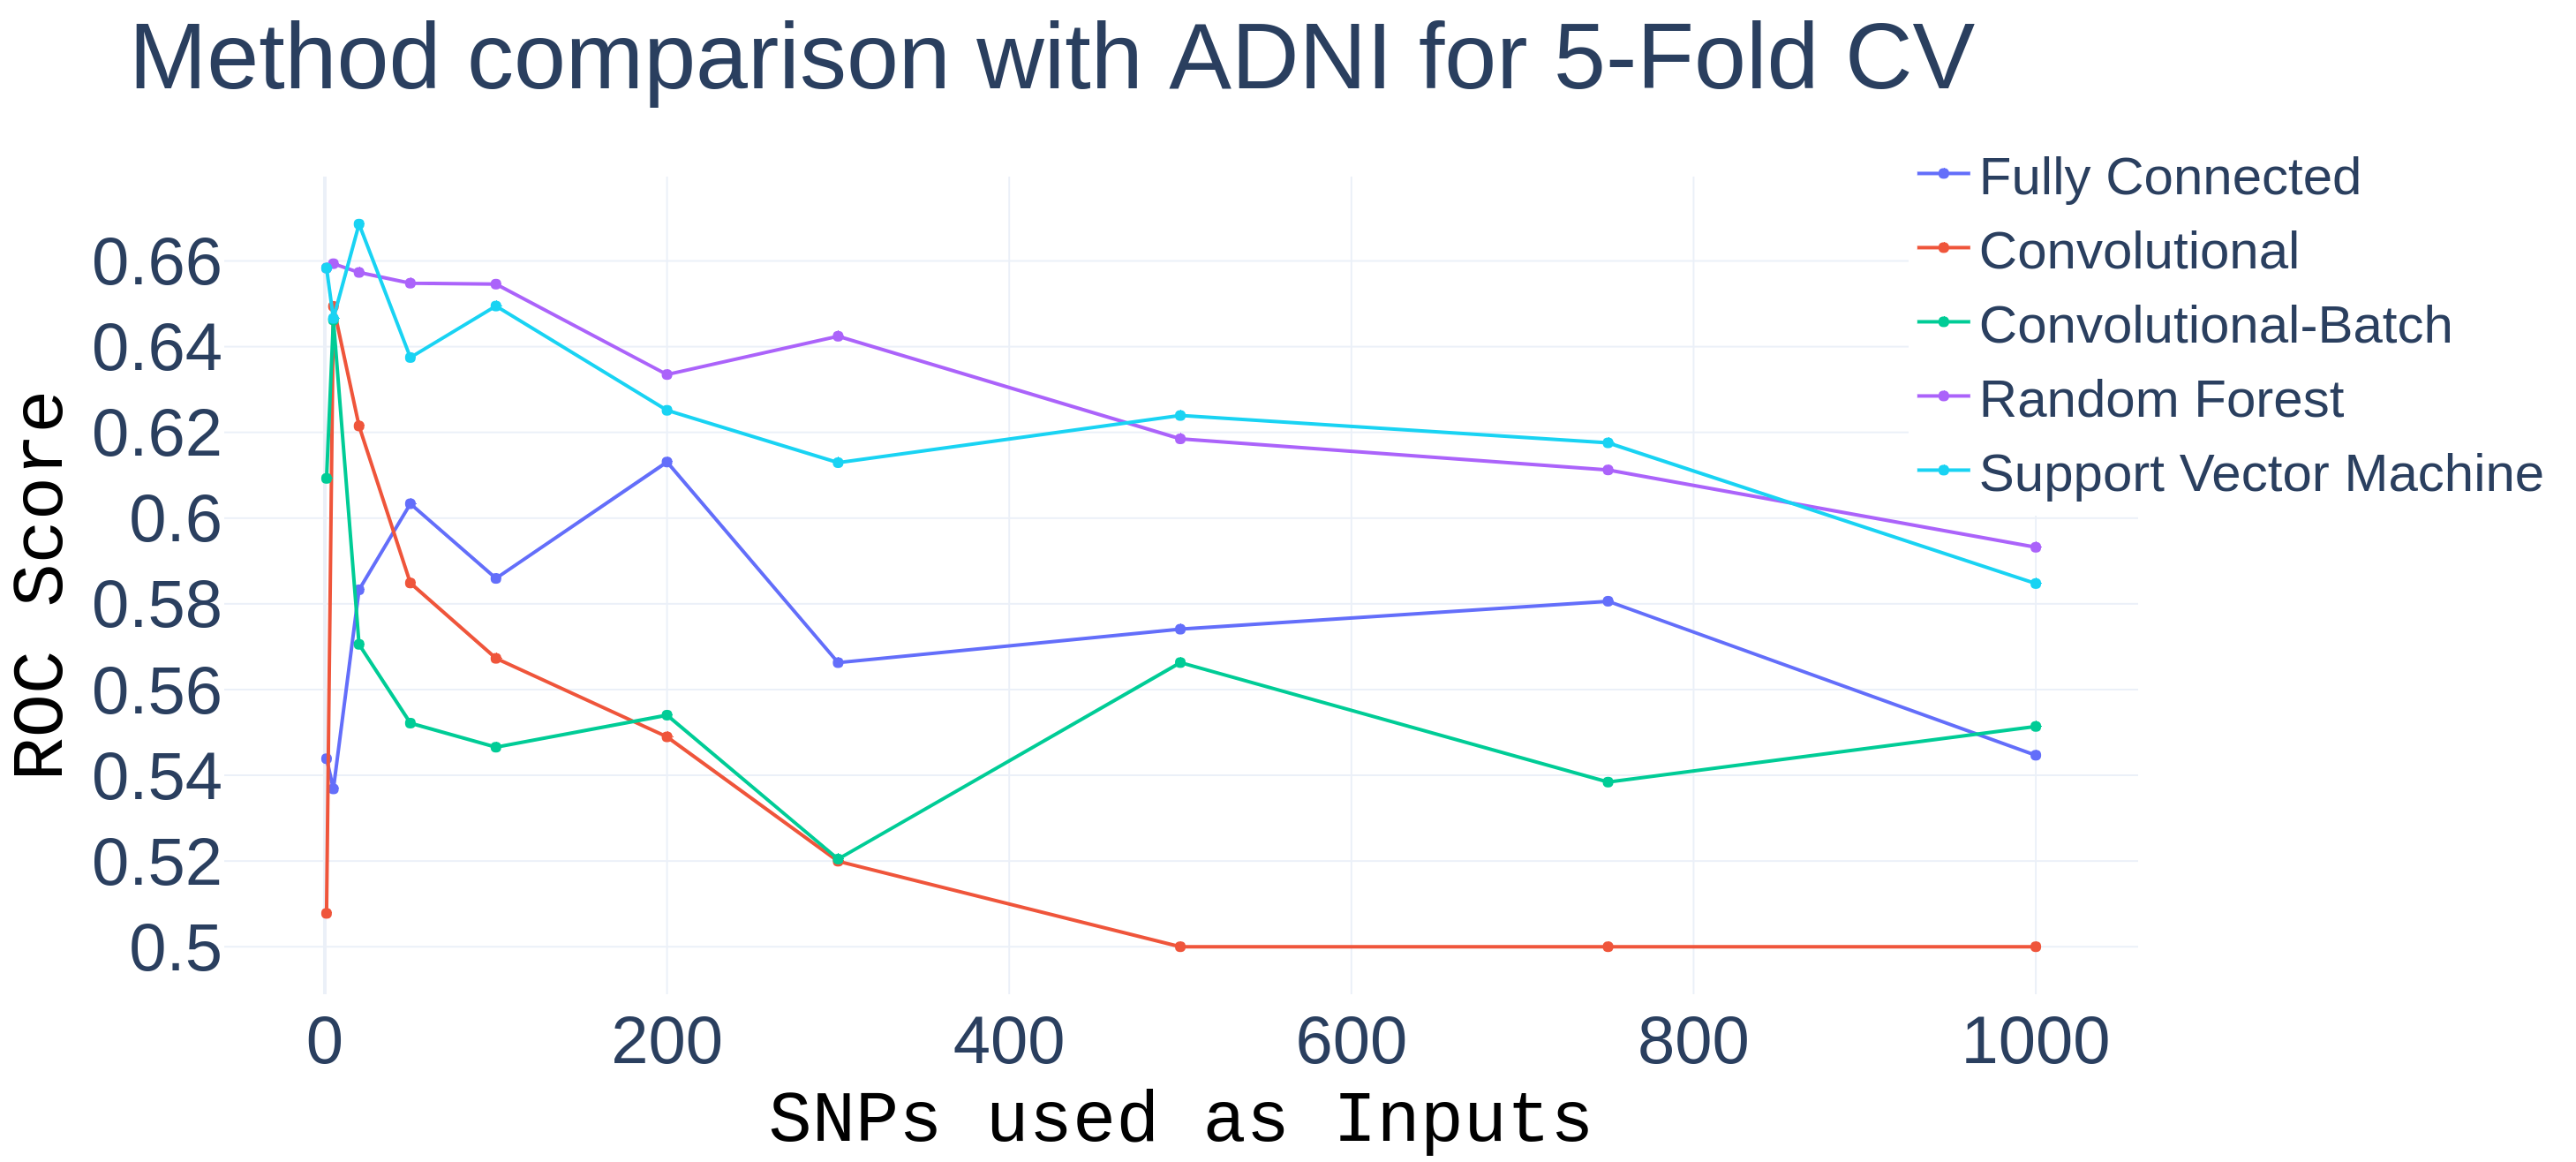
\includegraphics[width=4in]{images/results/AdniCV.png}}
\caption{{\bf Method comparison using the Complete ADNI dataset}
Analysis of the performance in terms of ROC AUC Score of the different classification methods when increasing the number of SNPs used as inputs, using 5-fold CV with the complete ADNI dataset .The SNPs used are in a descending order of statistical importance, with lower p-values as the first SNPs.}
\label{fig4}
\end{figure}

% Place figure captions after the first paragraph in which they are cited.
\begin{figure}[!ht]
\centerline{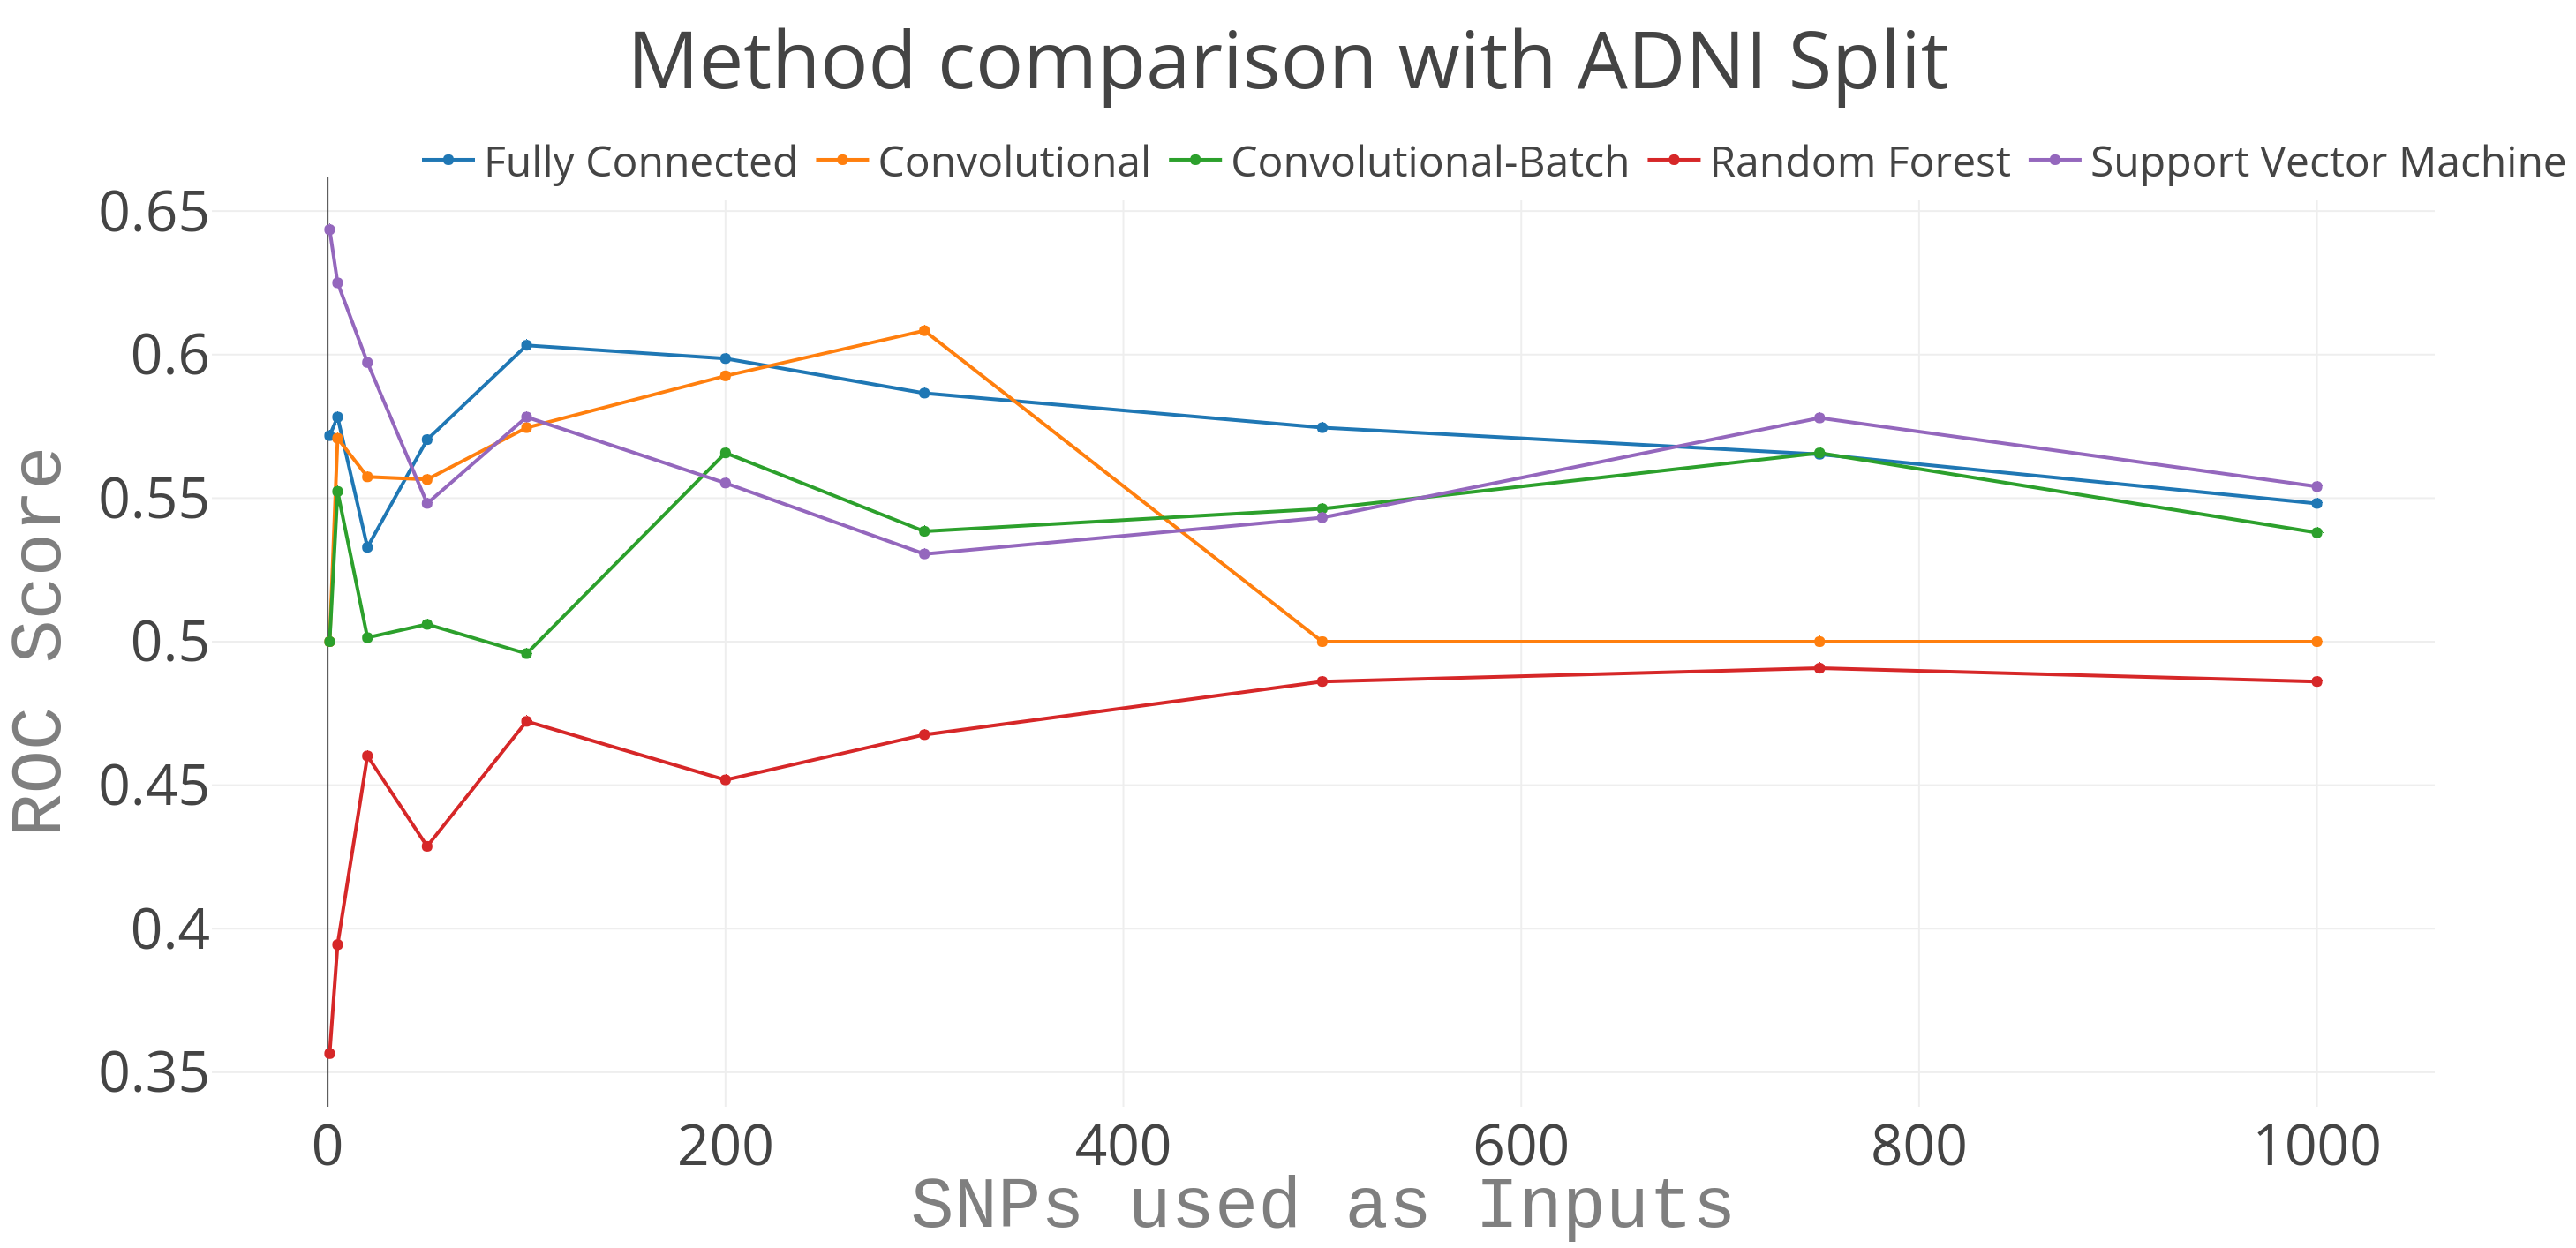
\includegraphics[width=4in]{images/results/AdniSplit2.png}}
\caption{{\bf Method comparison using the Split ADNI dataset}
Analysis of the performance in terms of ROC AUC Score of the different classification methods when increasing the number of SNPs used as inputs, training the model on the ADNI1 and ADNI GO samples and testing it in the IGAP-independent ADNI 2 Samples. }
\label{fig5}
\end{figure}

\section{Simulation}

The next step taken is to attempt to simulate a disease and find out the performance of the methods when utilizing a larger data set. With the simulation it can be clearly seen that the use of a higher number of data samples leads to a much more precise classification as shown in Figure 6. And more interestingly, the increase in the number of samples and makes it so that using a higher number of SNPs as input becomes more valuable. Thus with small data sets it makes sense to use the highest-rated SNPs, but by introducing more SNPs in large data sets the results are refined further and a more precise classification can be achieved. This can be seen in Figures 4.3, and 4.4. For a direct contrast between the performance using two different subsets (500 and 10,000 respectively) Figure 4.5 and 4.6 can be analyzed to see how the performance increase is substantial.


% Place figure captions after the first paragraph in which they are cited.
\begin{figure}[!ht]
\centerline{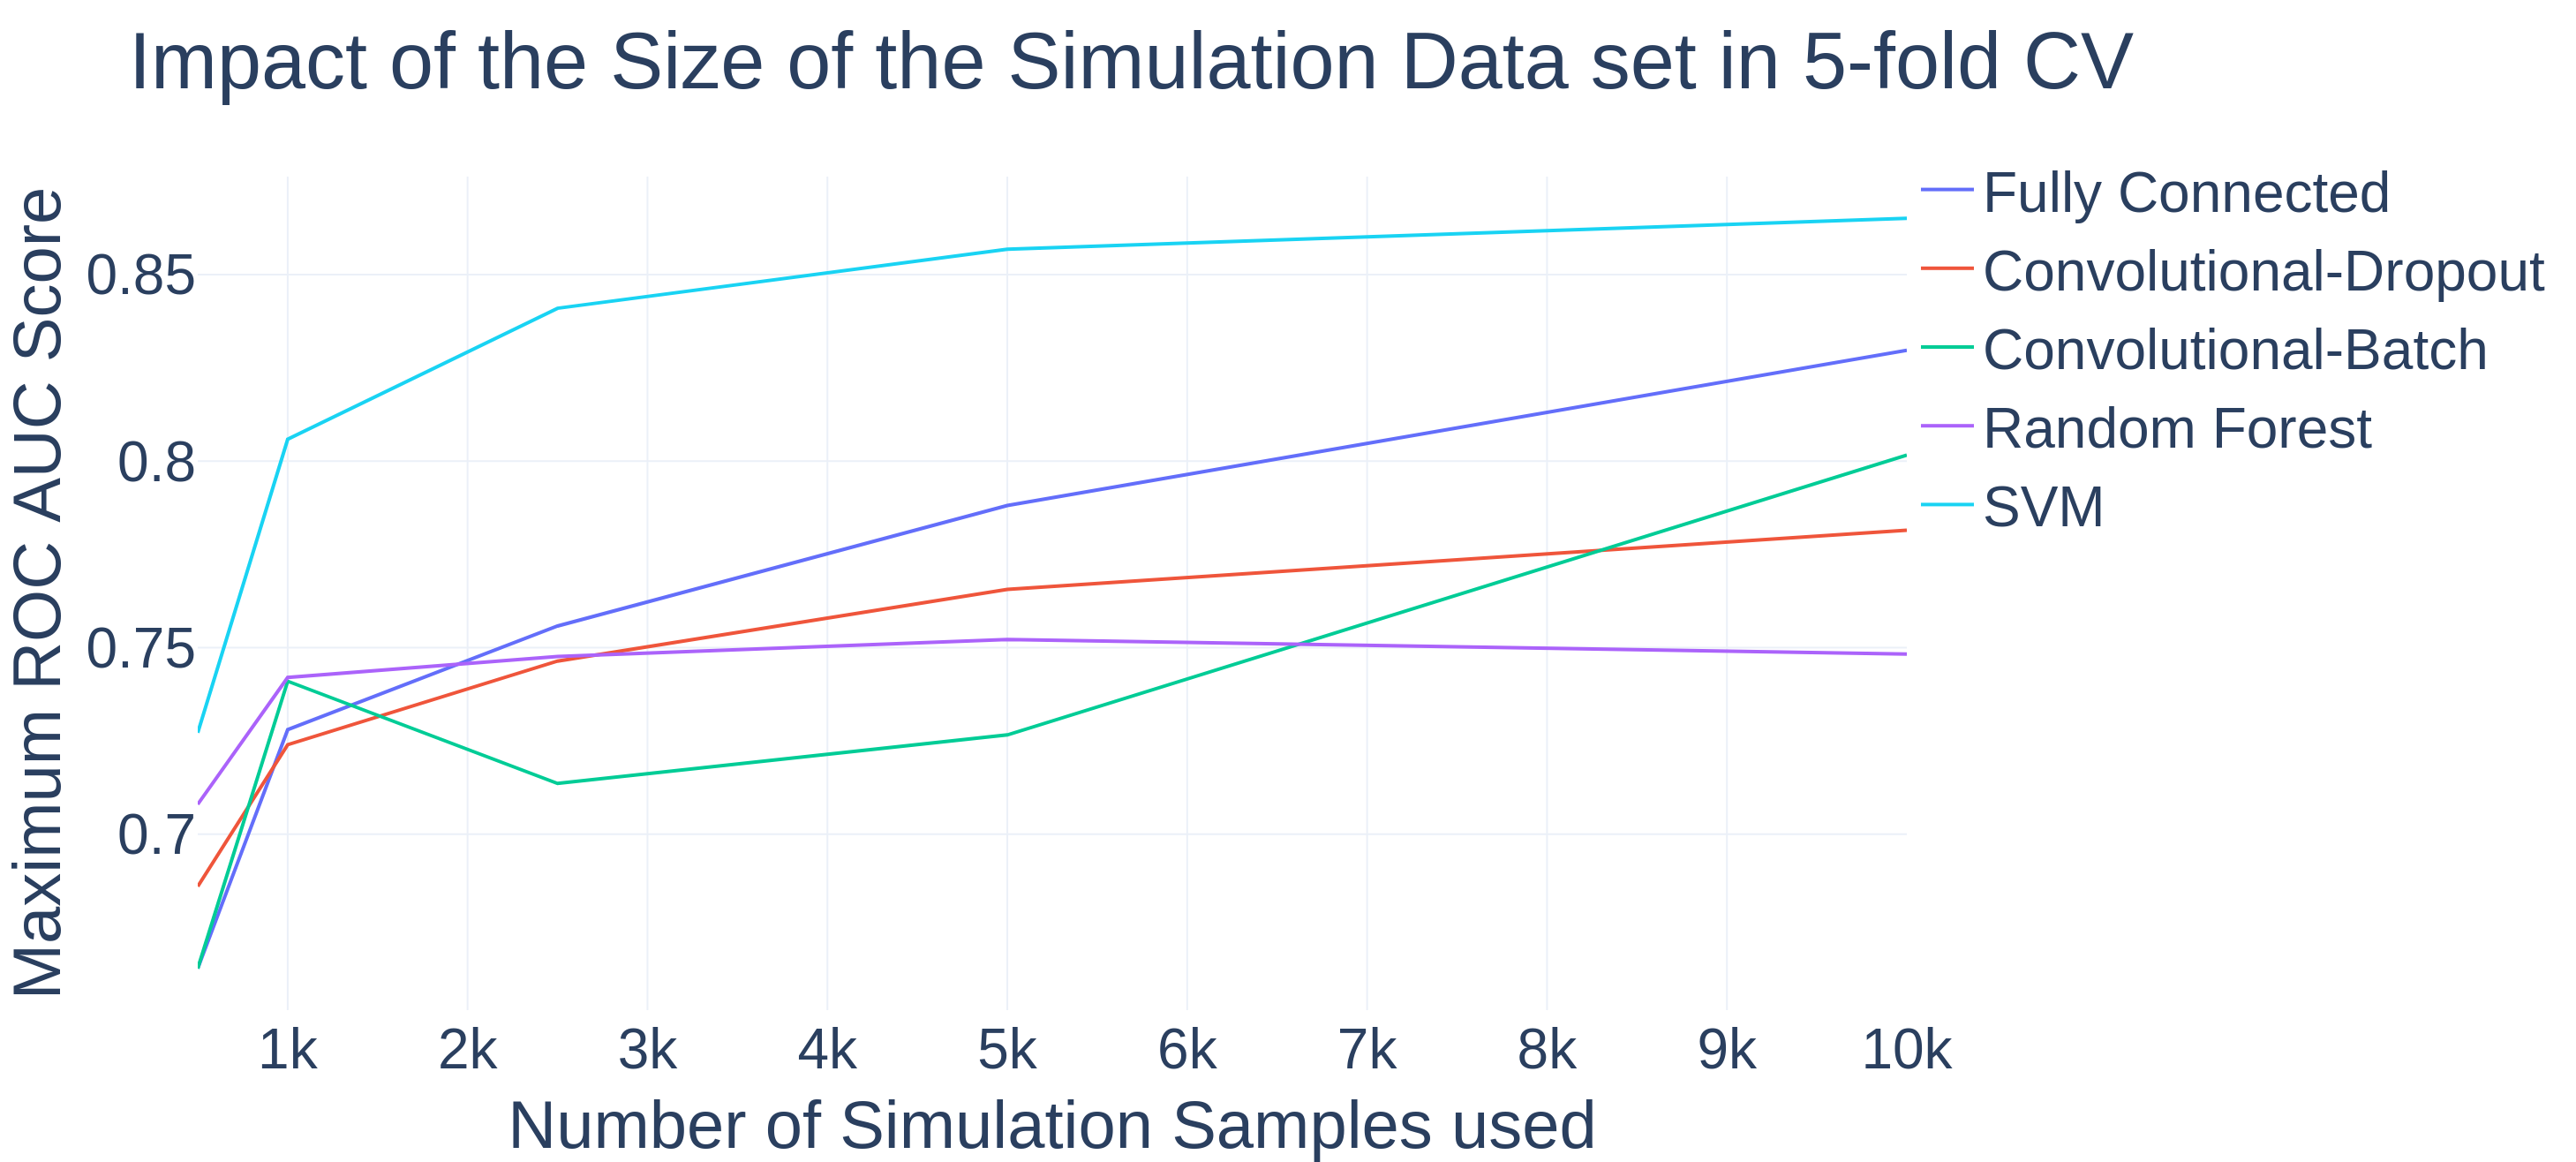
\includegraphics[width=4in]{images/results/ImpactSim.png}}
\caption{{\bf Impact of the subset size on the prediction}
Analysis of the effect in the ROC AUC Score done by increasing the number of samples used for the 5-fold CV in the simulated dataset using the different classification methods.}
\label{fig6}
\end{figure}

\begin{figure}[!ht]
\centerline{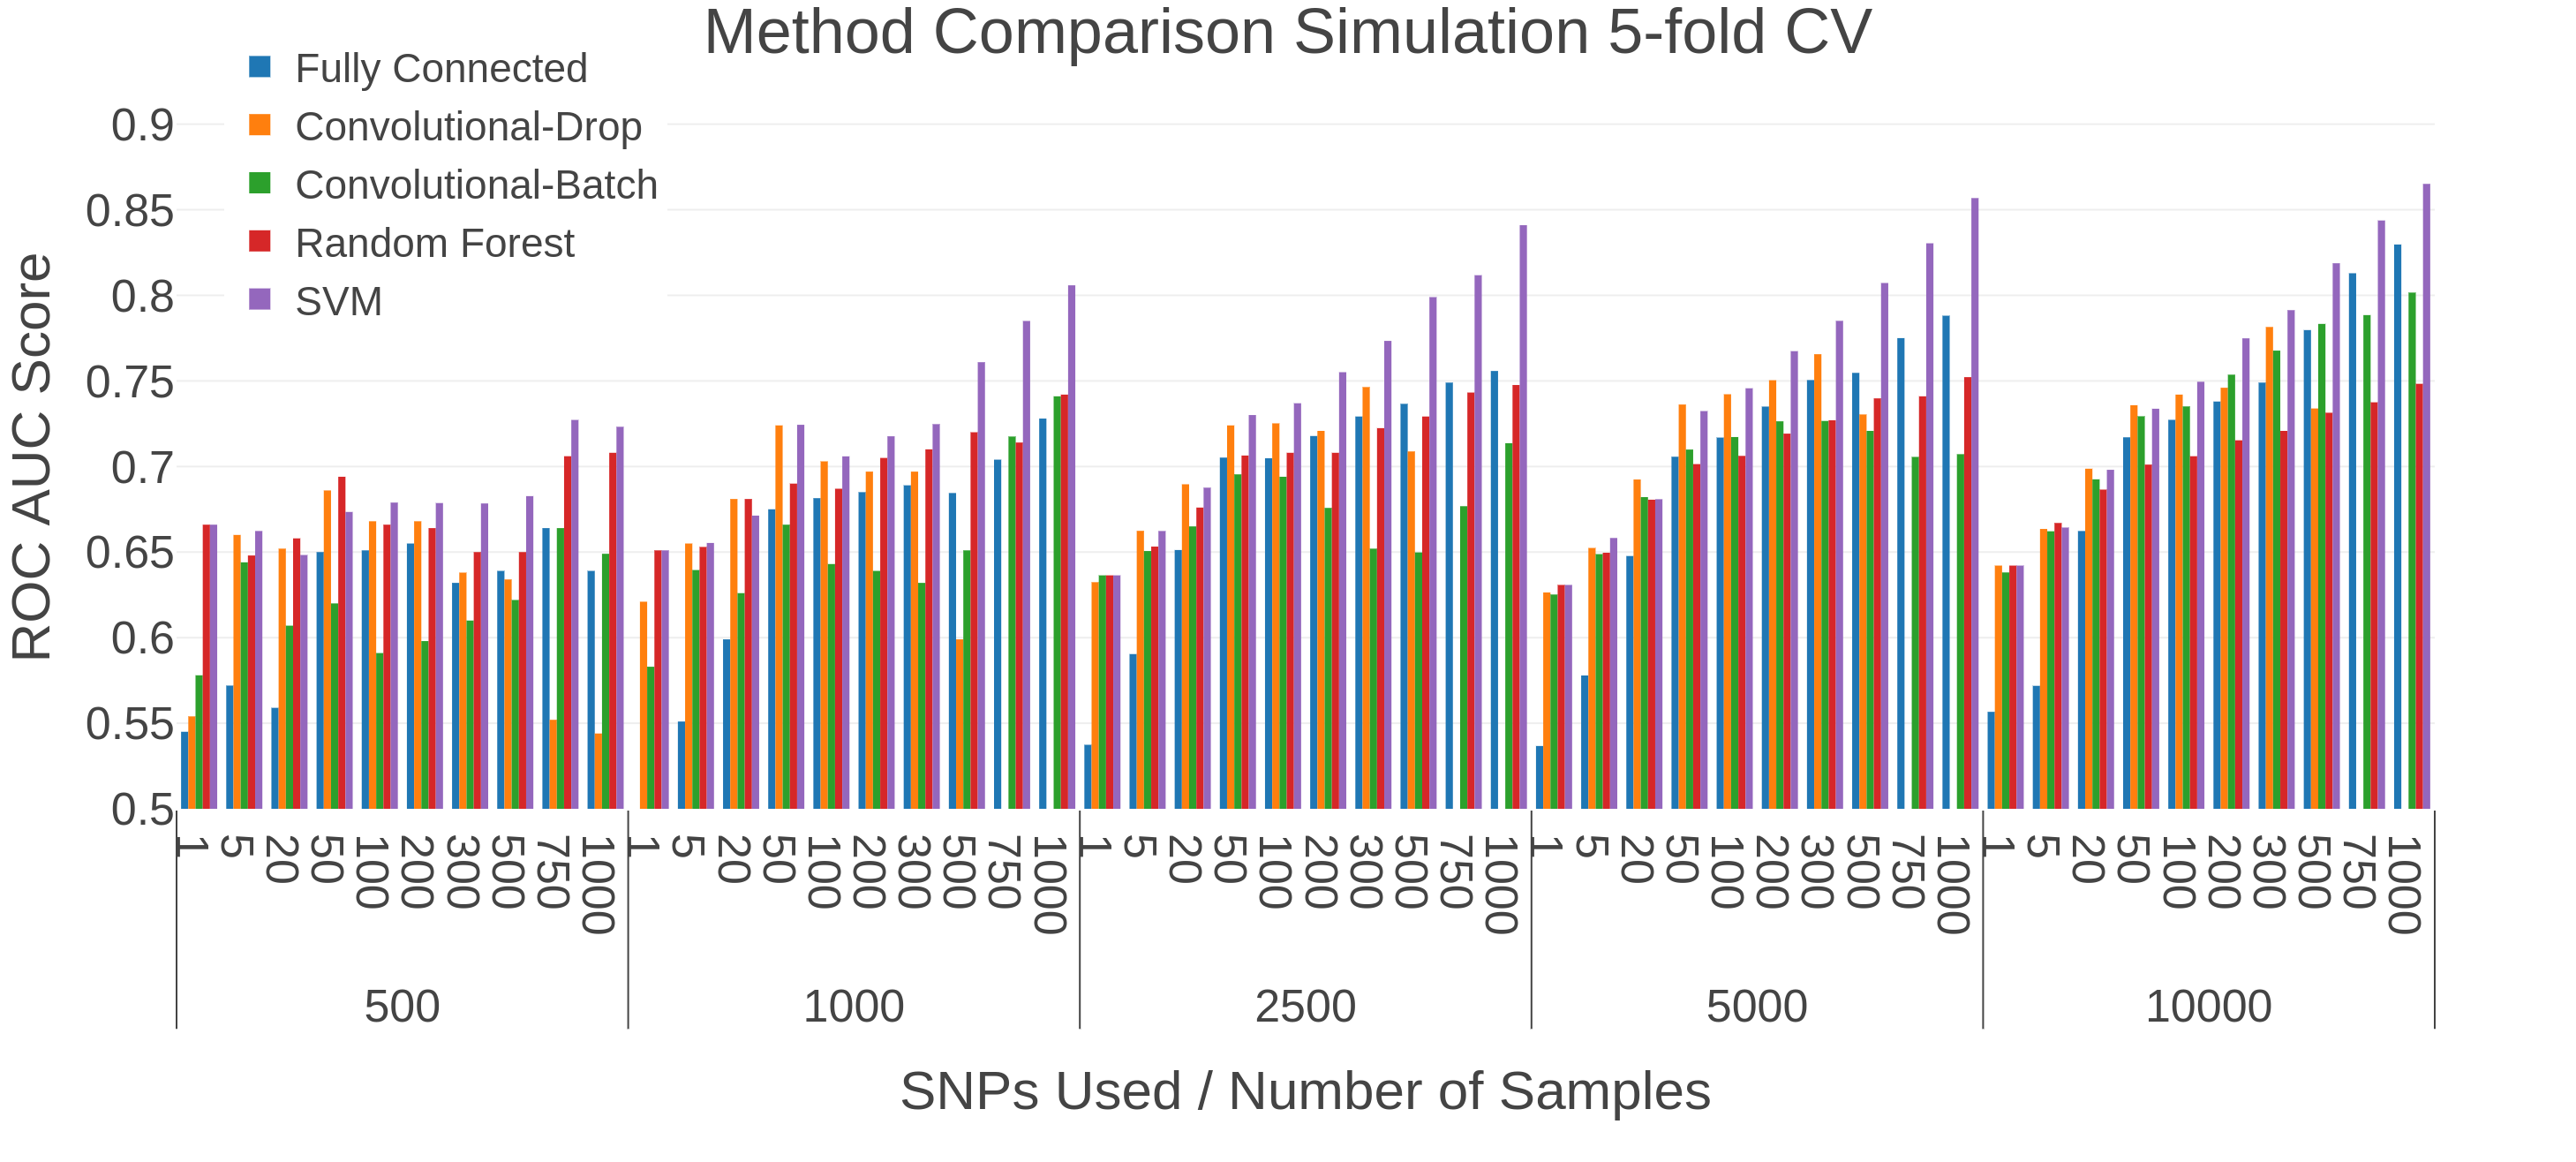
\includegraphics[width=4in]{images/results/SimComplete.png}}
\caption{{\bf Method Comparison with Simulated Dataset}
Comparison between the ROC AUC Score obtained using the different classification methods. The X axis firstly describes an increase of the number of SNPS used for classification, and afterwards an increase in the size of the simulation dataset}
\label{fig7}
\end{figure}


\begin{figure}[!ht]
\centerline{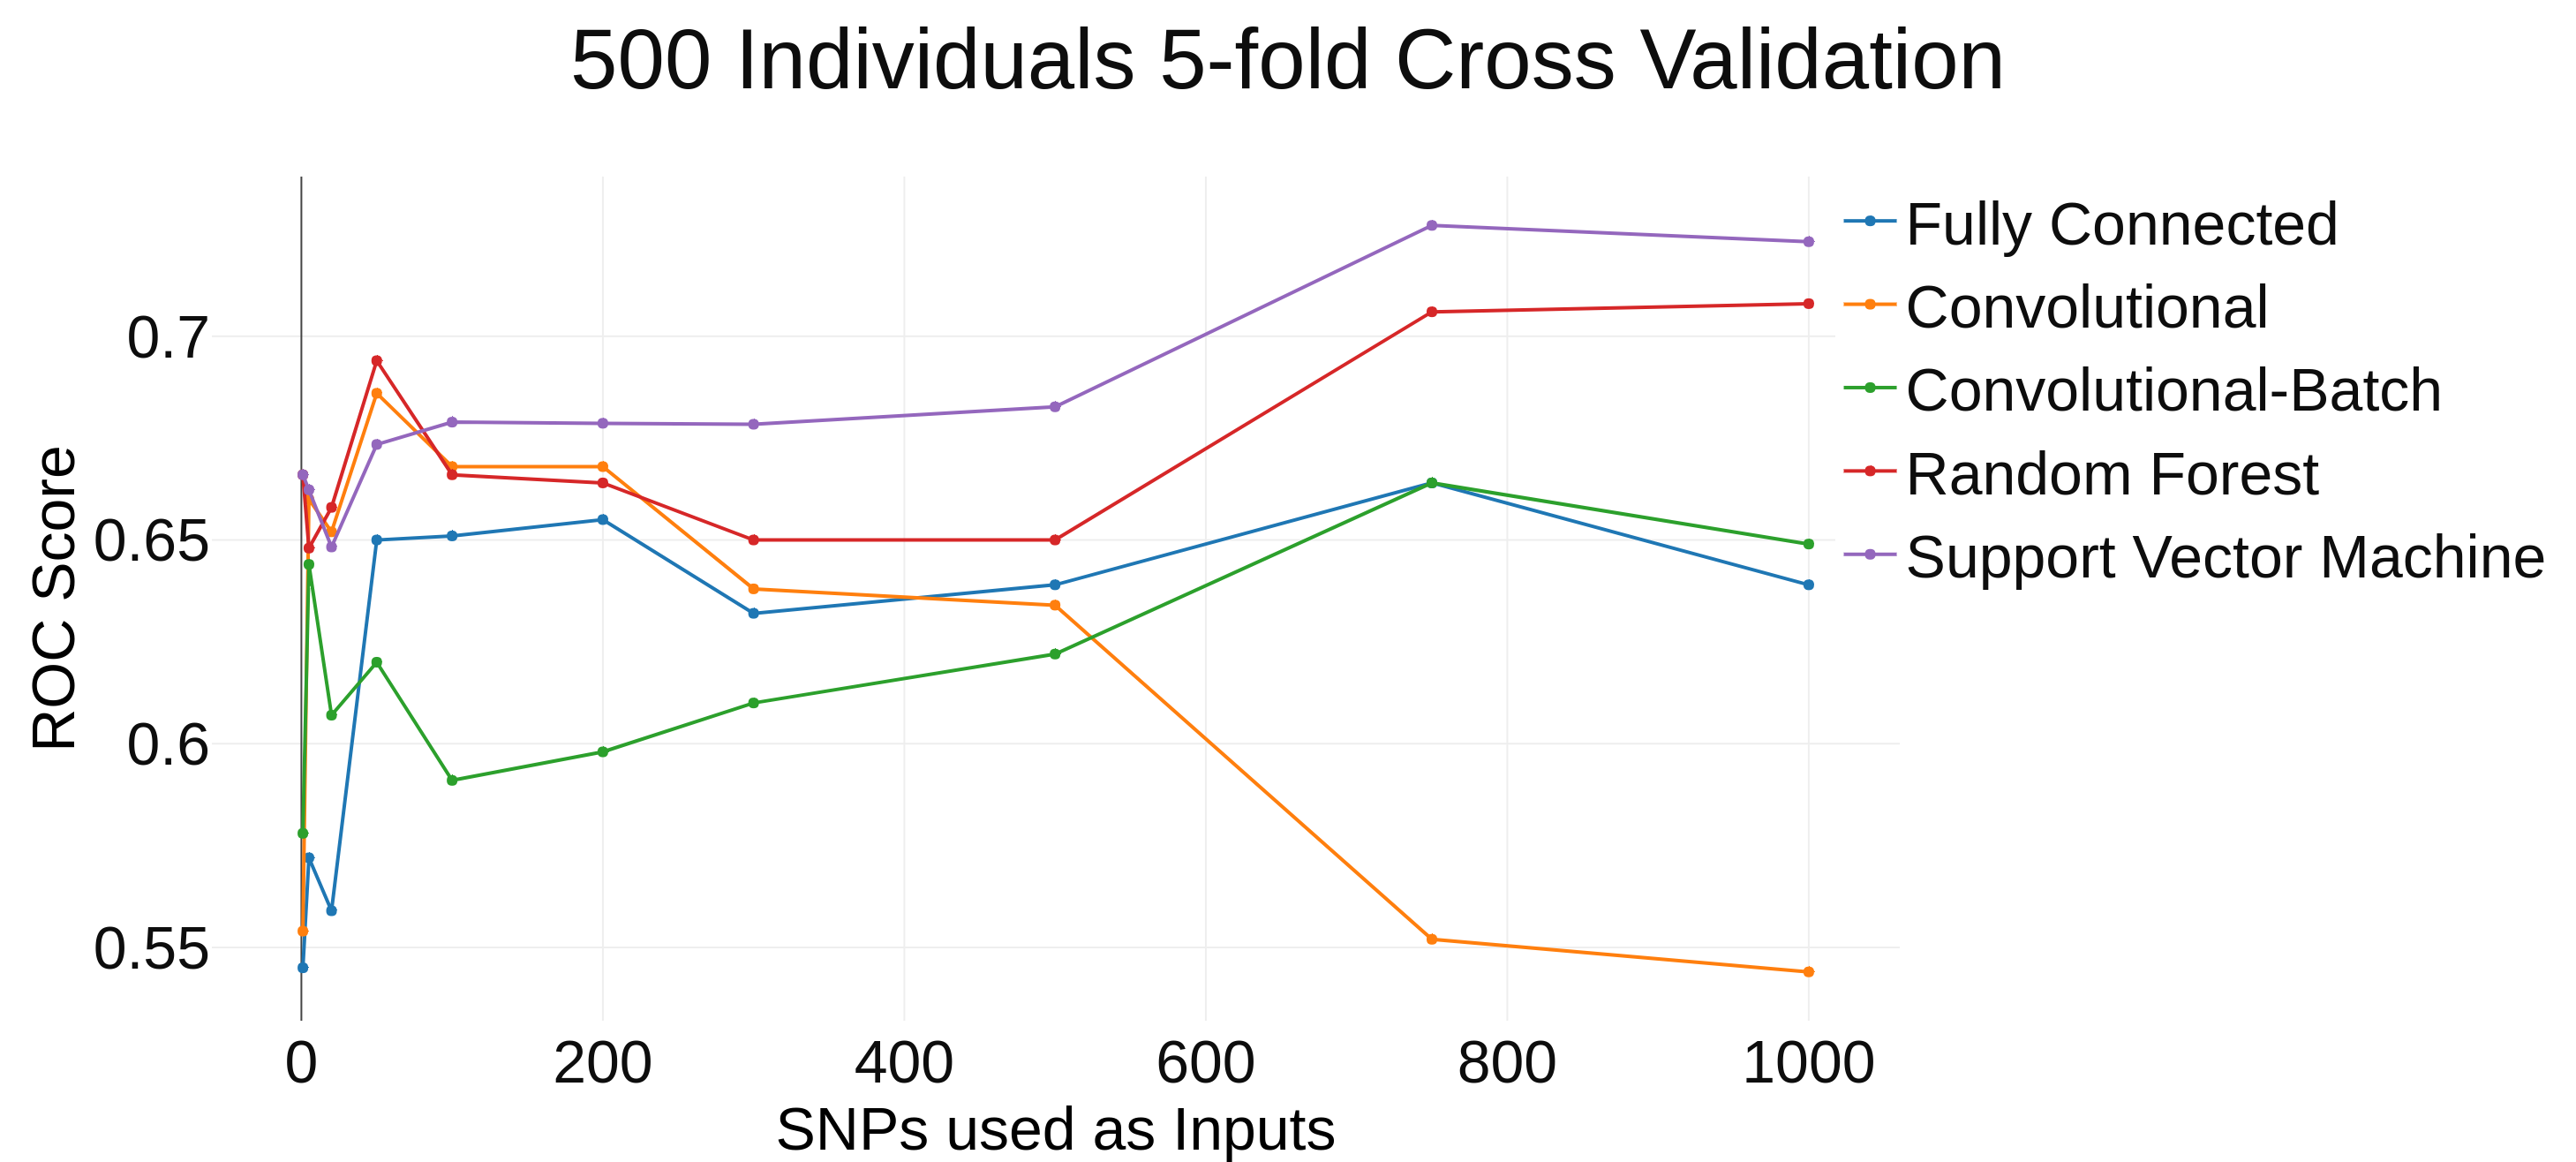
\includegraphics[width=4in]{images/results/Sim500.png}}
\caption{{\bf Method comparison with 500 Individuals}
Comparison of the ROC AUC Score from 5-fold CV using different classification methods while increasing the number of SNPs given a simulation dataset with 500 Individuals}
\label{fig8}
\end{figure}

\begin{figure}[!ht]
\centerline{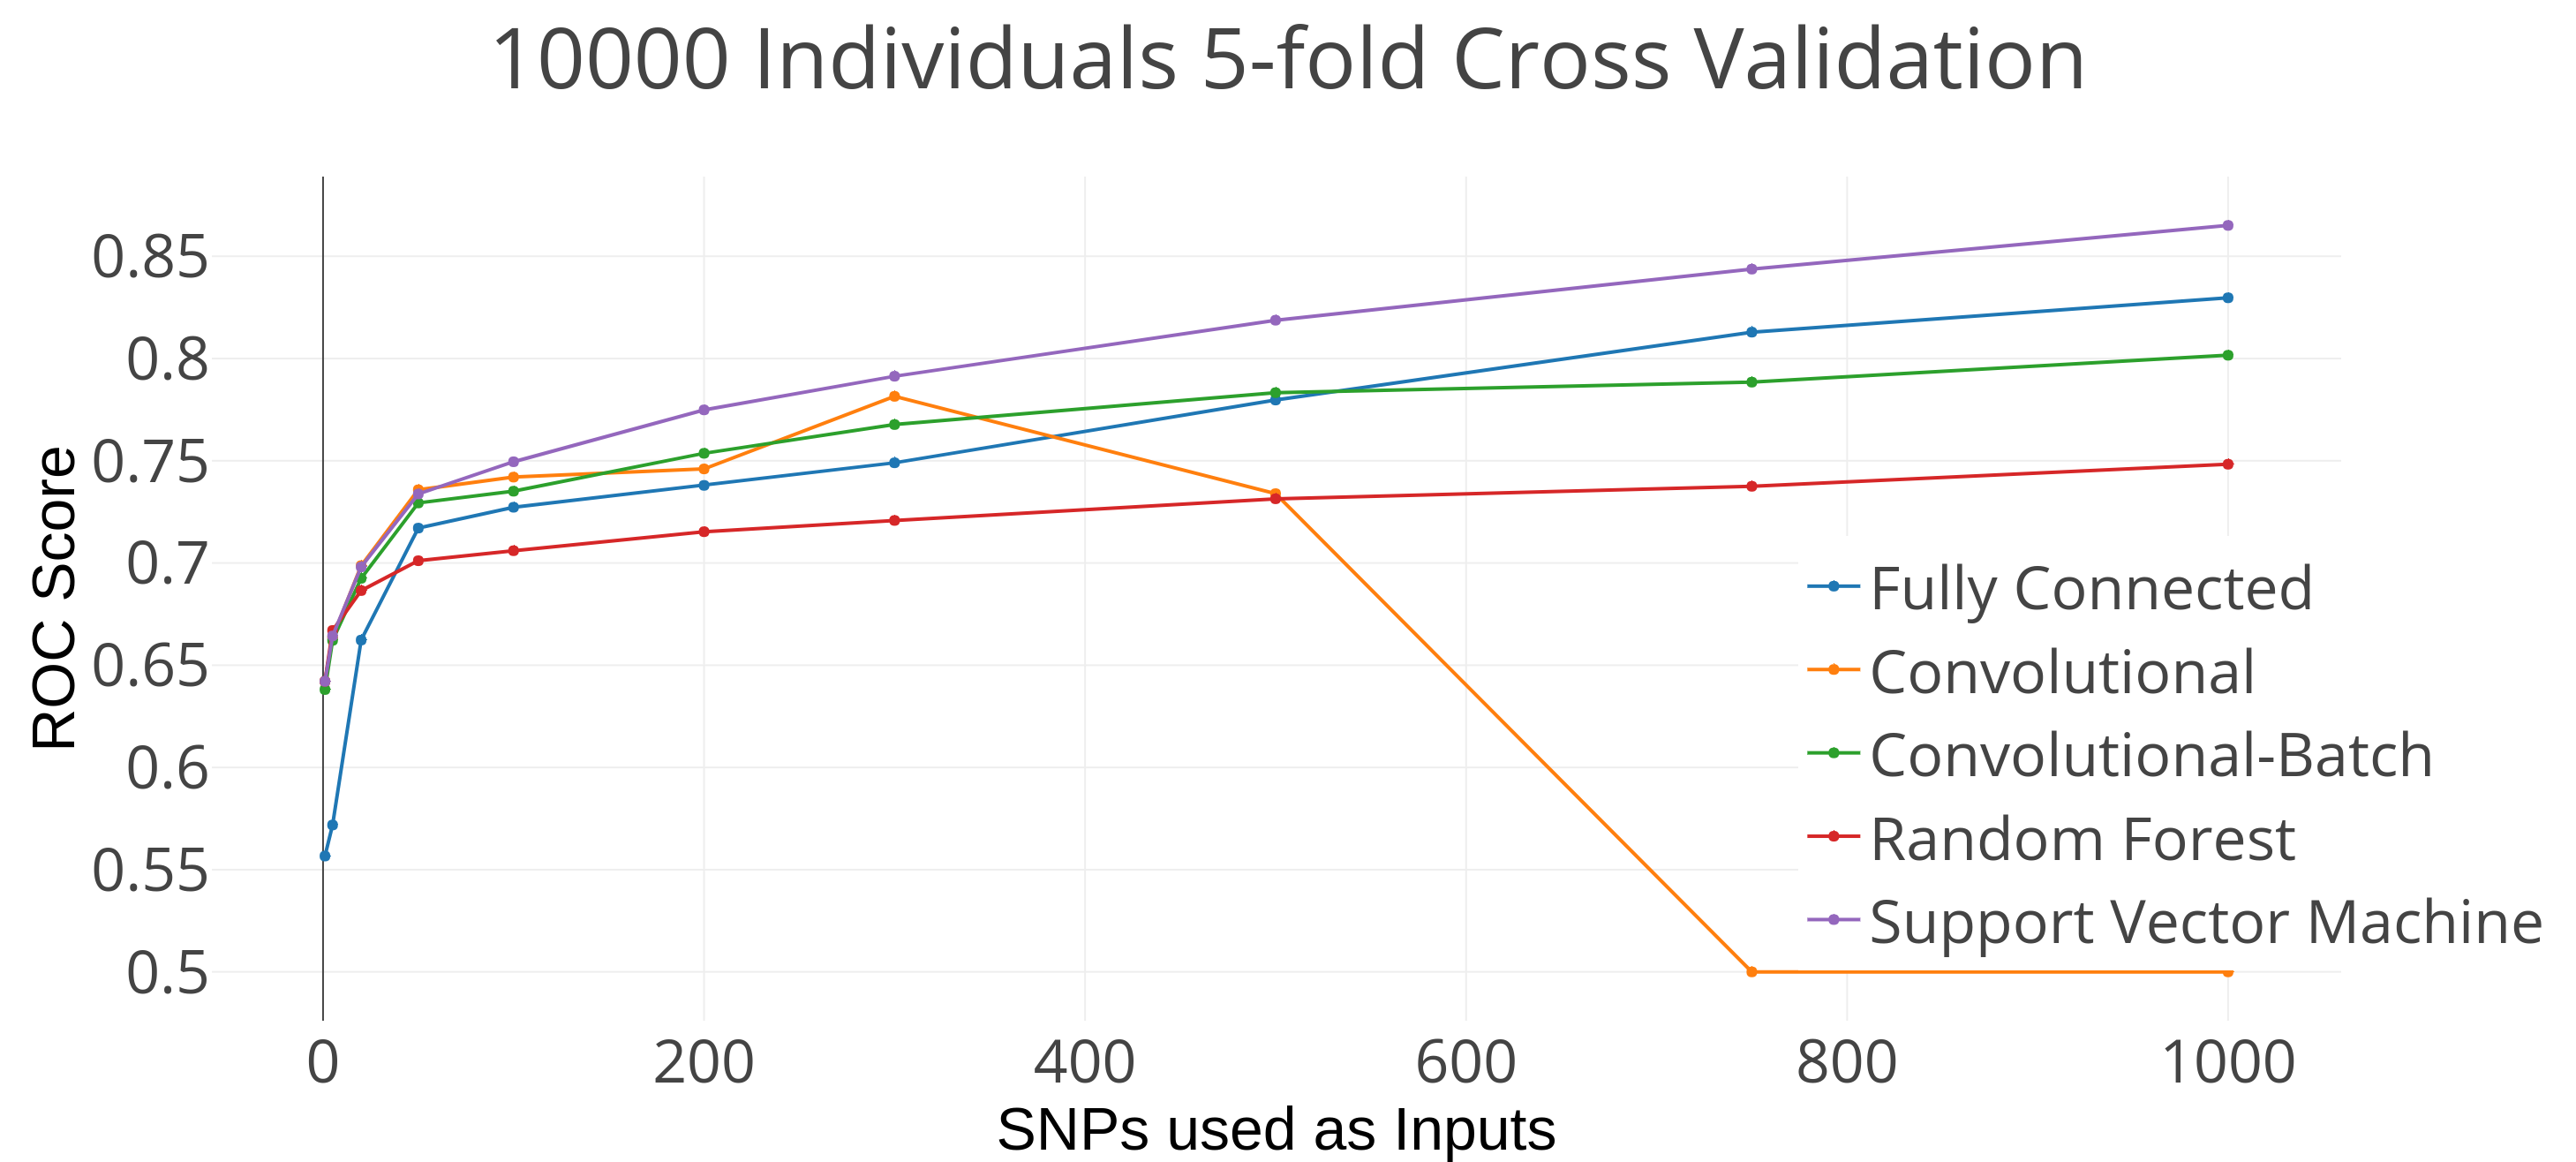
\includegraphics[width=4in]{images/results/Sim10000.png}}
\caption{{\bf Method comparison with 10000 Individuals}
Comparison of the ROC AUC Score from 5-fold CV using different classification methods while increasing the number of SNPs given a simulation dataset with 10,000 Individuals}
\label{fig9}
\end{figure}
\clearpage
\section{Data Augmentation}

The results from the previous simulation show that the use of more samples should benefit the prediction in the Alzheimer's task. Thus,  the artificially augmented data set is generated for training purposes and used the ADNI data set as the test set. In this case the increase in the number of samples did not directly mean a better performance and a higher use of SNPs, as it can be seen, once the system starts using over 100 SNPs the performance on the ADNI subset tends to decay. Plus, the increase in size of the training data set also did not mean constant increases as in the previous scenario. It is shown that the use of more SNPs coupled with a decent size of artificially-augmented samples gives the best results on the ROC Score, which shows that both of these factors have a role to play in the prediction. The convolutional dropout network did have some issues when using too much SNPs and dropped to a classification, and in general the simpler models such as Random Forest and Support Vector Machine performed better. This shows that there is only so much that can be accomplished with data augmentation, and that the disease might actually be focused on a smaller number of uncorrelated genes as supposed in the simulation. Figures 4.7 and 4.8 illustrate these results.

% Place figure captions after the first paragraph in which they are cited.
\begin{figure}[!ht]
\centerline{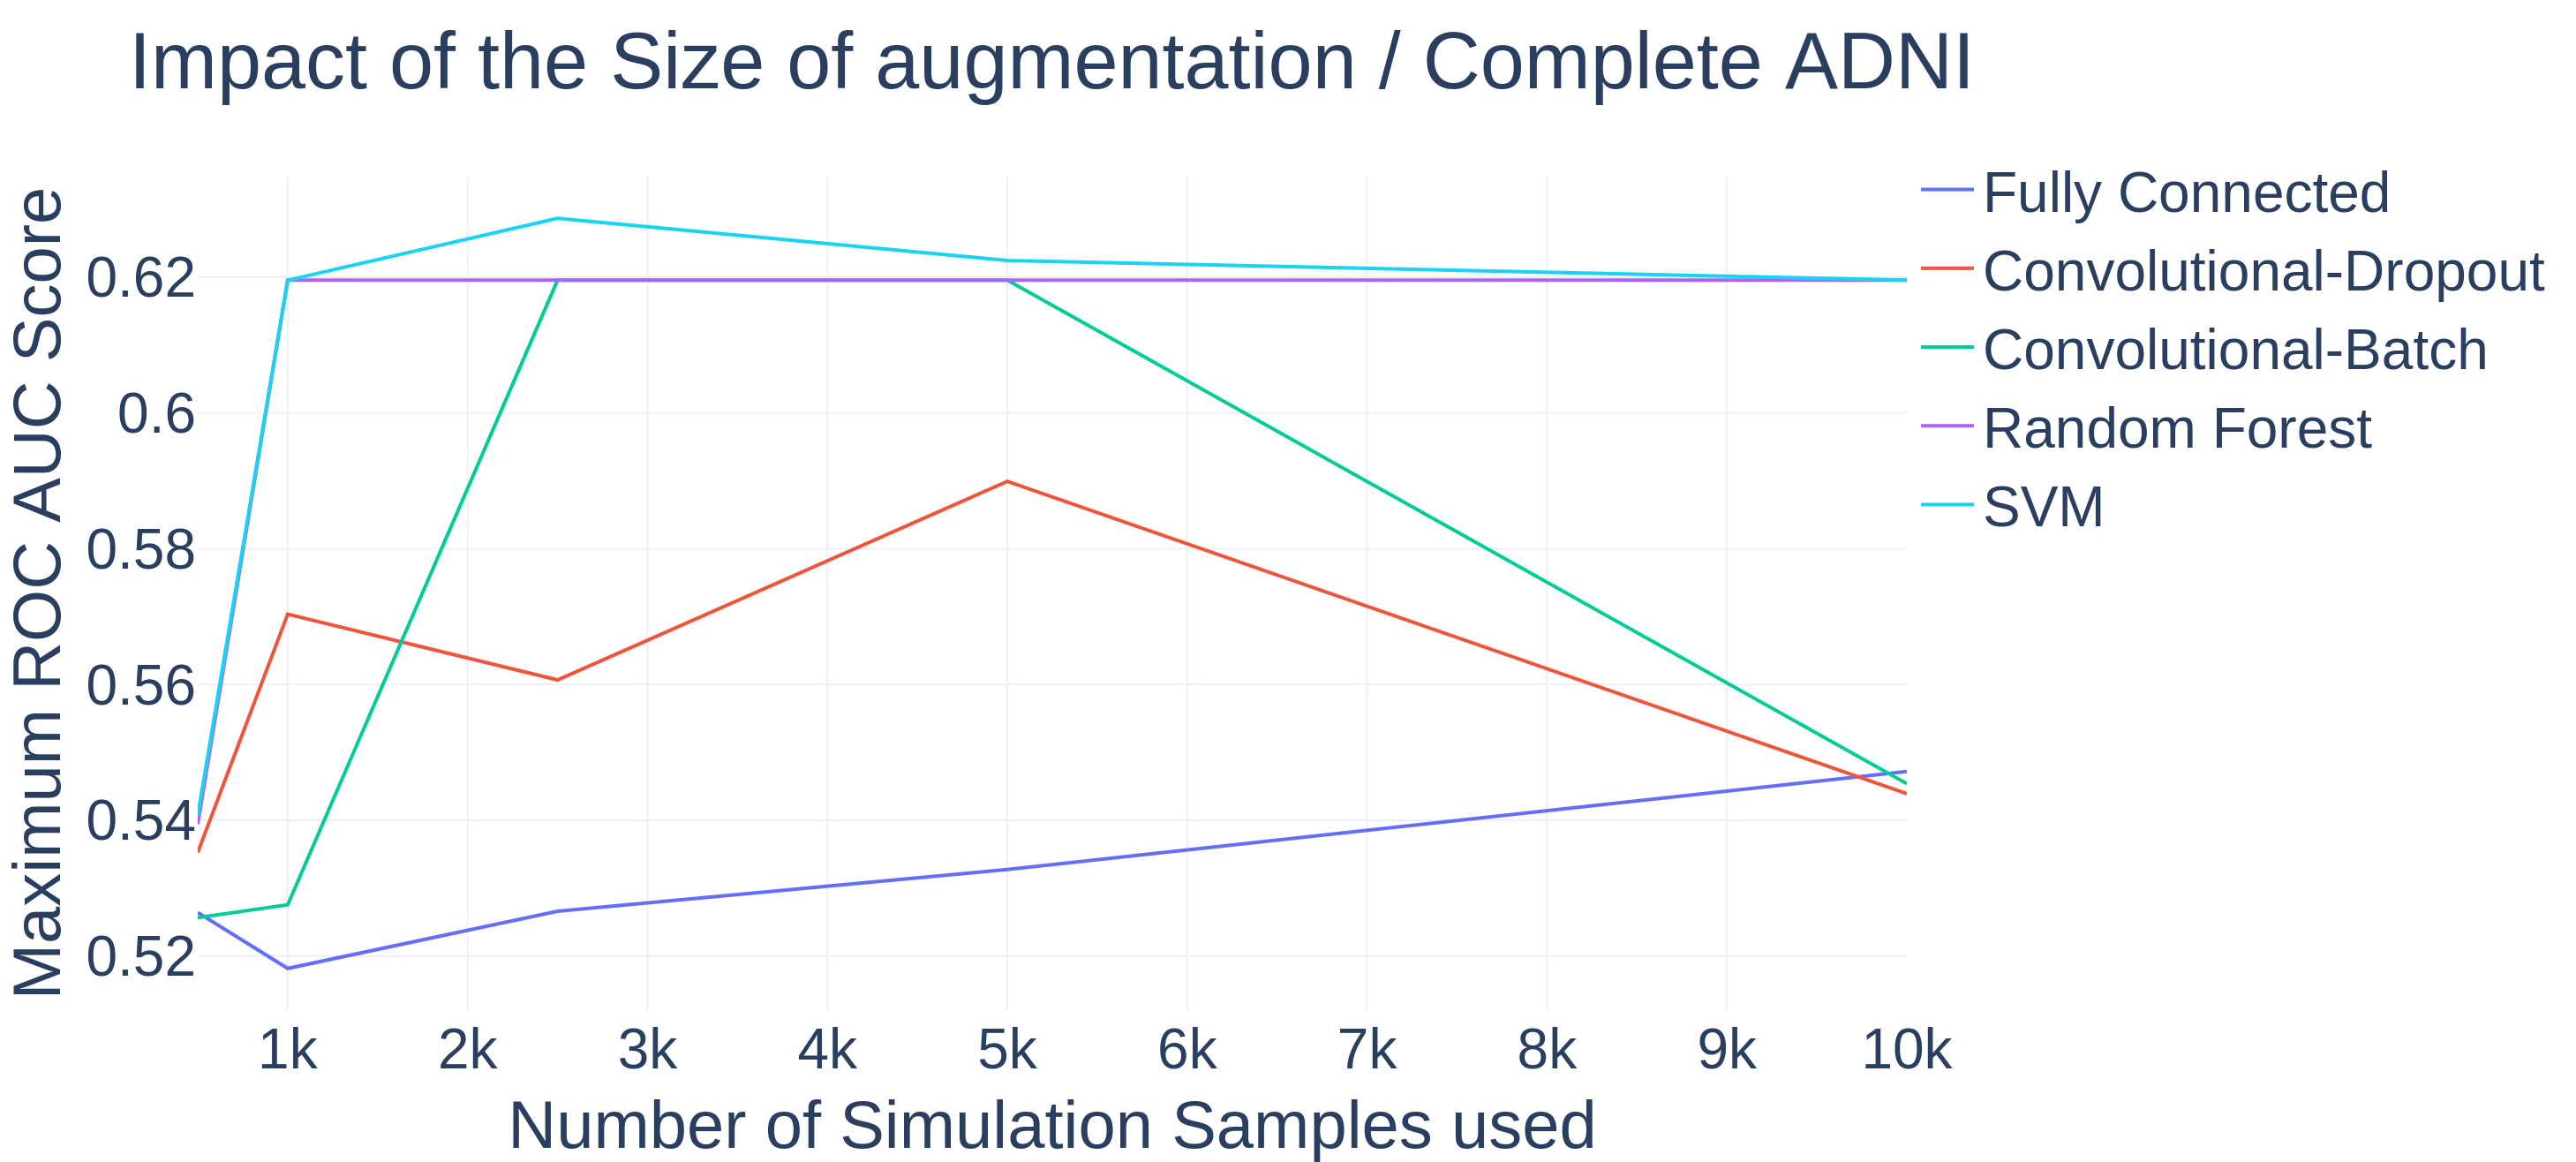
\includegraphics[width=4in]{images/results/ImpactDataAug.png}}
\caption{{\bf Impact of the augmentation size on the prediction}
Analysis of the effect in the ROC AUC Score done by increasing the number of data-augmentation samples used for the training segment validated on the complete ADNI Dataset using the different classification methods.}
\label{fig10}
\end{figure}

\begin{figure}[!ht]
\centerline{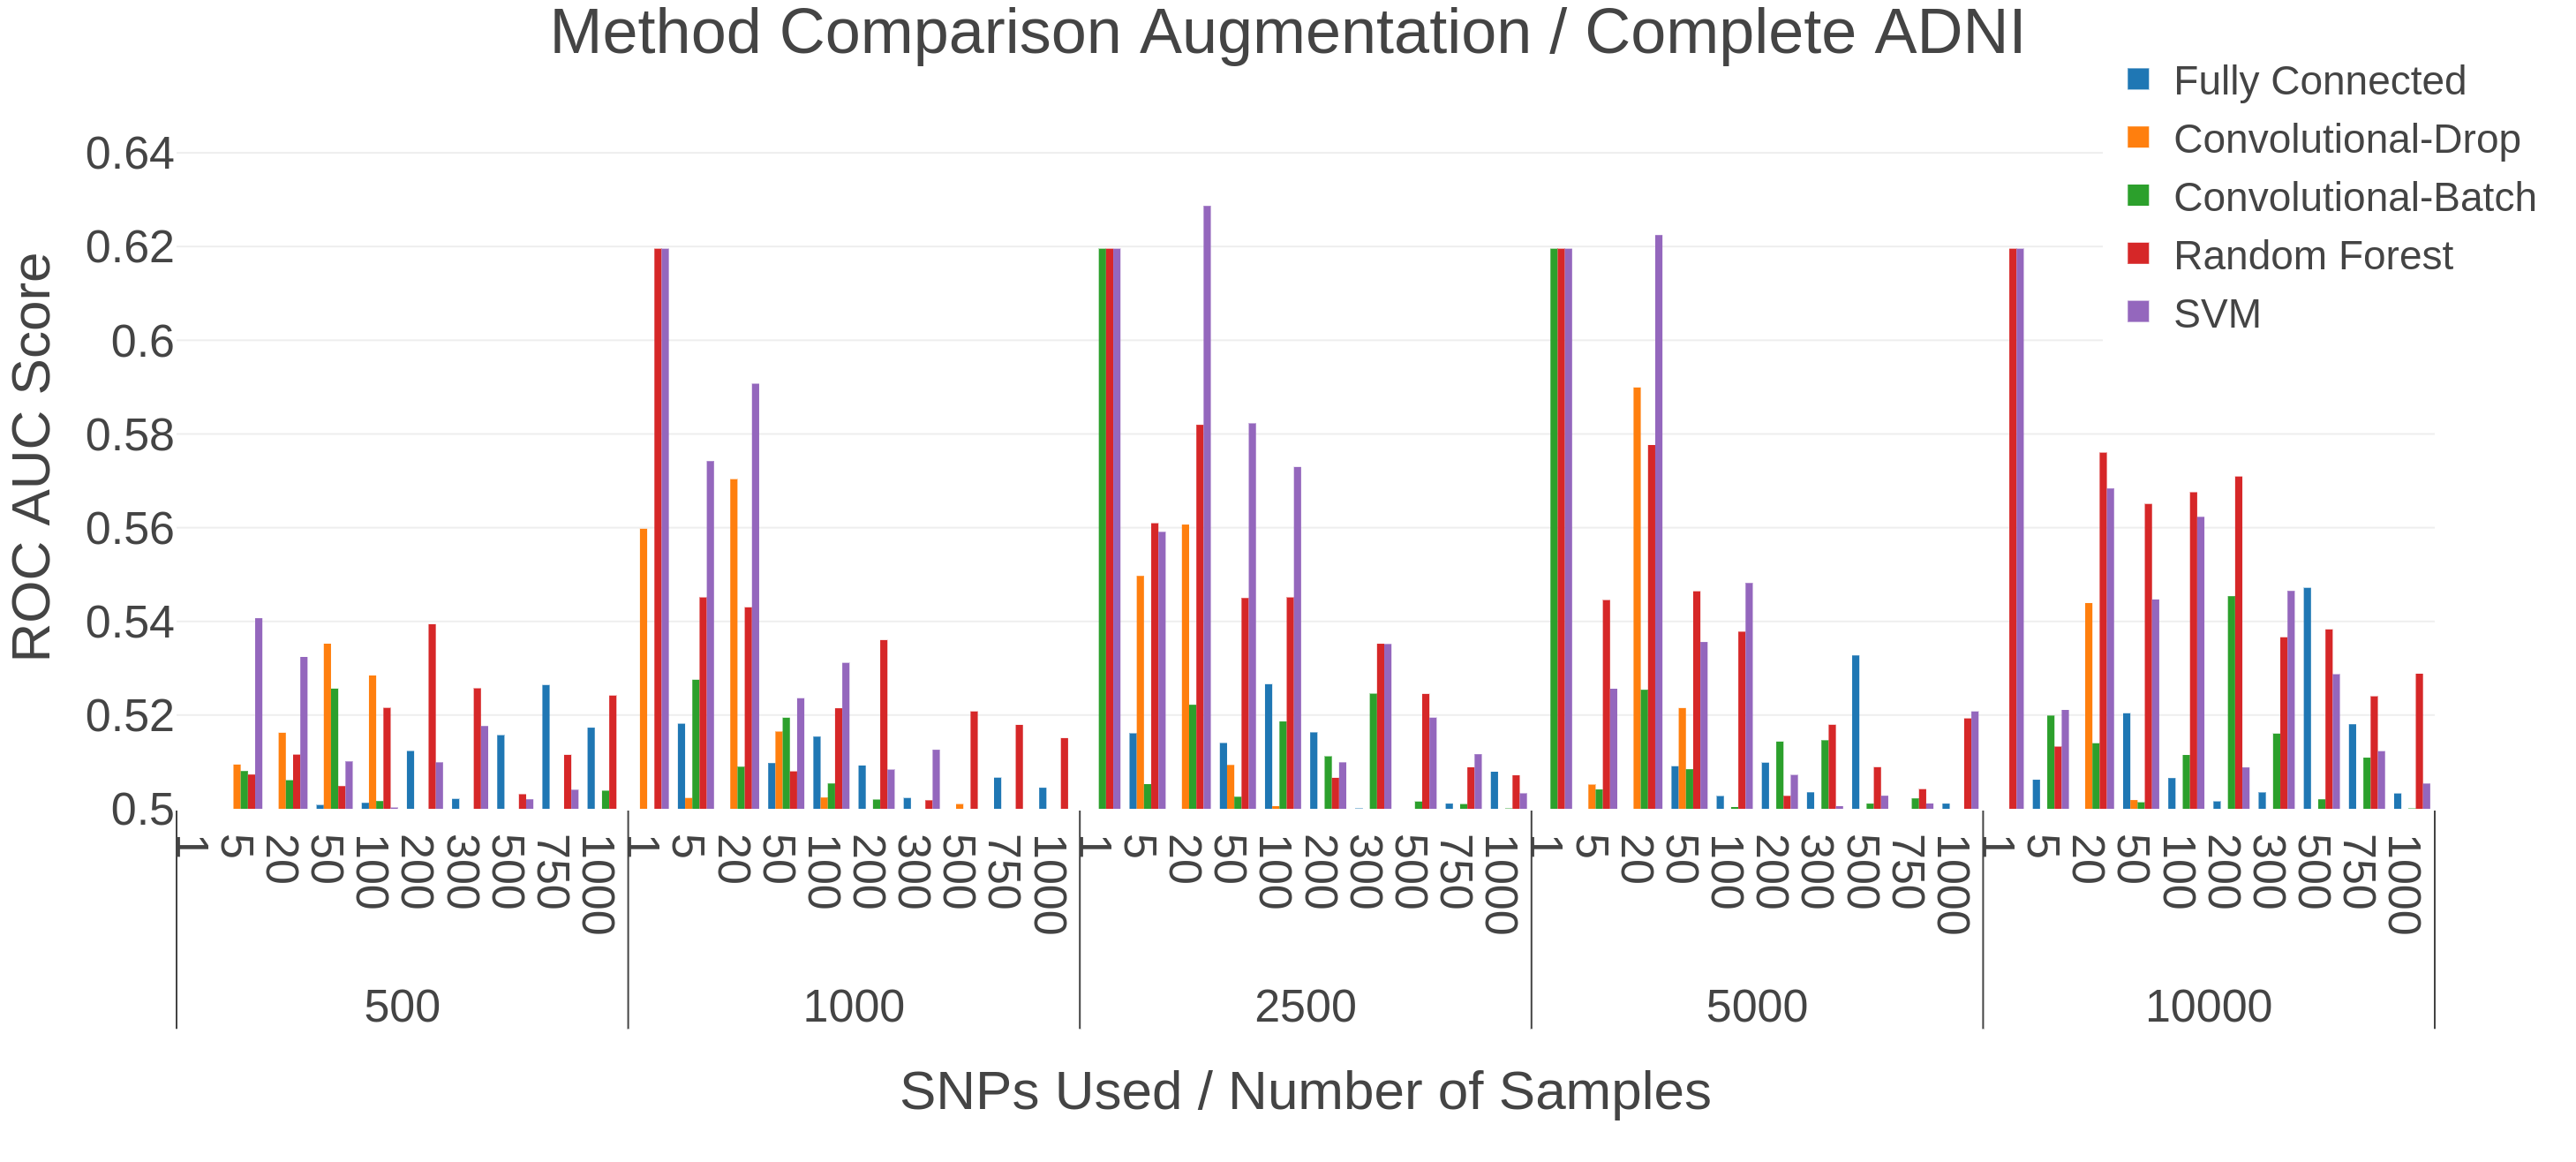
\includegraphics[width=4in]{images/results/DataAugComplete.png}}
\caption{{\bf Method Comparison with full ADNI Dataset} 
Comparison between the ROC AUC Score obtained using the different classification methods. The X axis firstly describes an increase of the number of SNPs used for classification, and afterwards an increase in the data-augmentation size validated on the complete ADNI dataset}
\label{fig11}
\end{figure}


Further restrictions are imposed on the data set used for testing, as some of the ADNI samples are also taken into account for the IGAP study. Thus the testing is restricted to those individuals who did not participate in the IGAP study. For this case it is shown in Figures 4.9 and 4.10 that due to the small sample size and the class imbalance the results are lower as the previous data set. Specifically they tend to show good results using few amounts of SNPs (APOE $\epsilon4$ mainly) and the increase in sample size used to train does not represent an increase in the prediction capability. This gives us the impression that the learning models either do not generalize correctly, or the few individuals from the unbalanced data set do not correspond to the genetic markers learned from the IGAP-based simulation. Comparing these results with the ones obtained from the ADNI split the results are in average better for the data augmentation process than from the standard. 

\begin{figure}[!ht]
\centerline{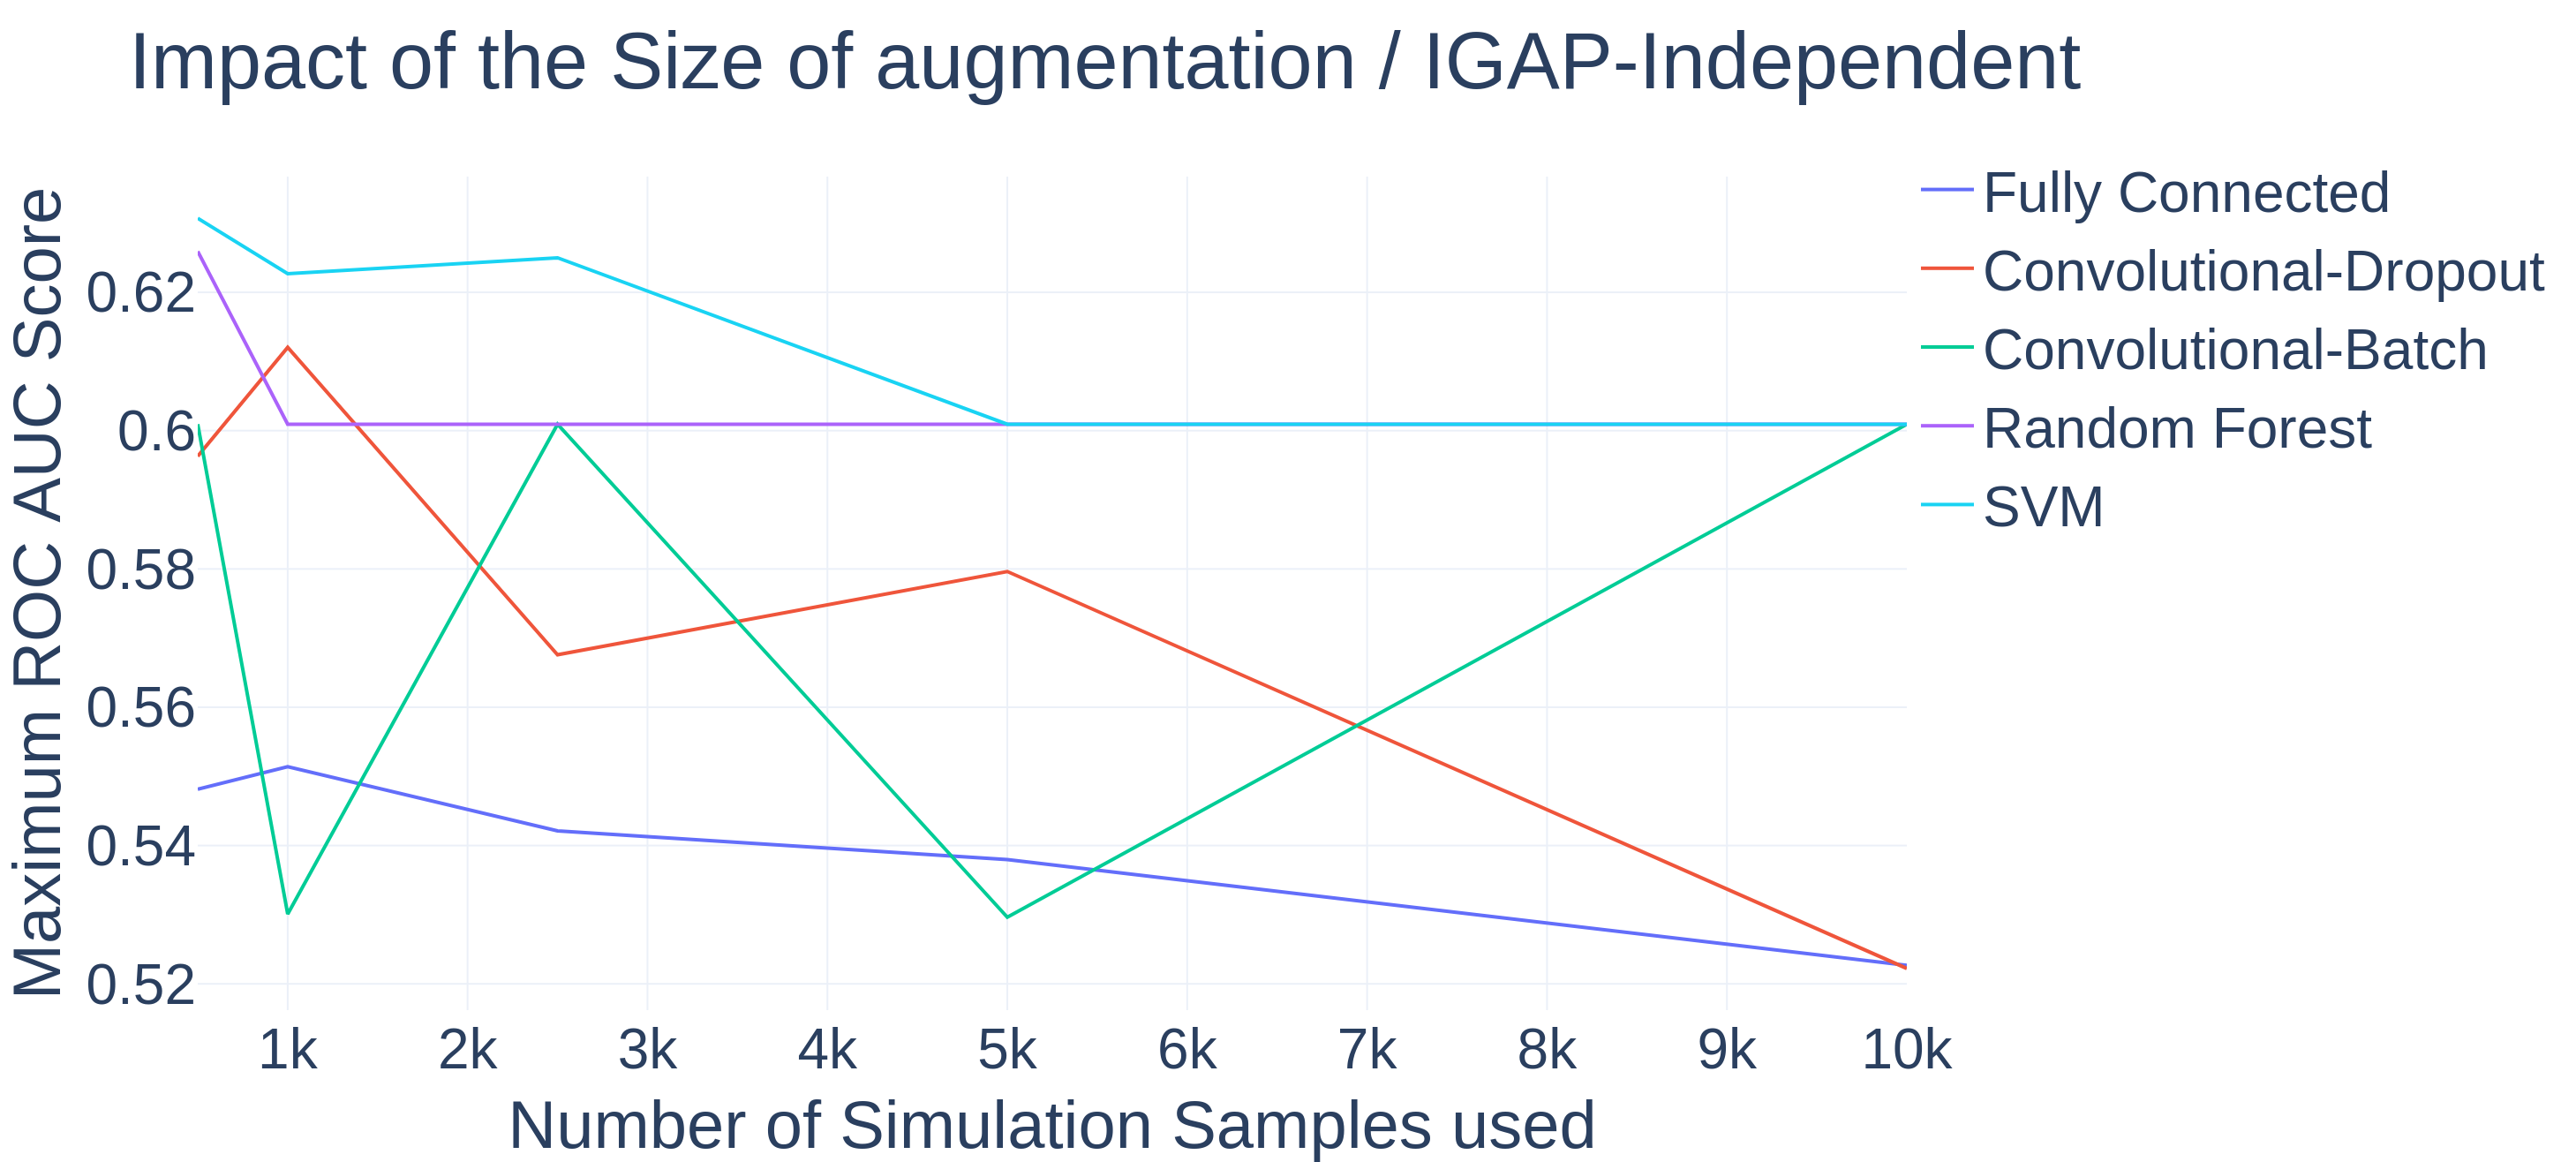
\includegraphics[width=4in]{images/results/ImpactDataAug2.png}}
\caption{{\bf Impact of the augmentation size in IGAP-Independent Subset}
Analysis of the effect in the ROC AUC Score done by increasing the number of data-augmentation samples used for the training segment validated on the IGAP-Independent subset using the different classification methods.}
\label{fig12}
\end{figure}

\begin{figure}[!ht]
\centerline{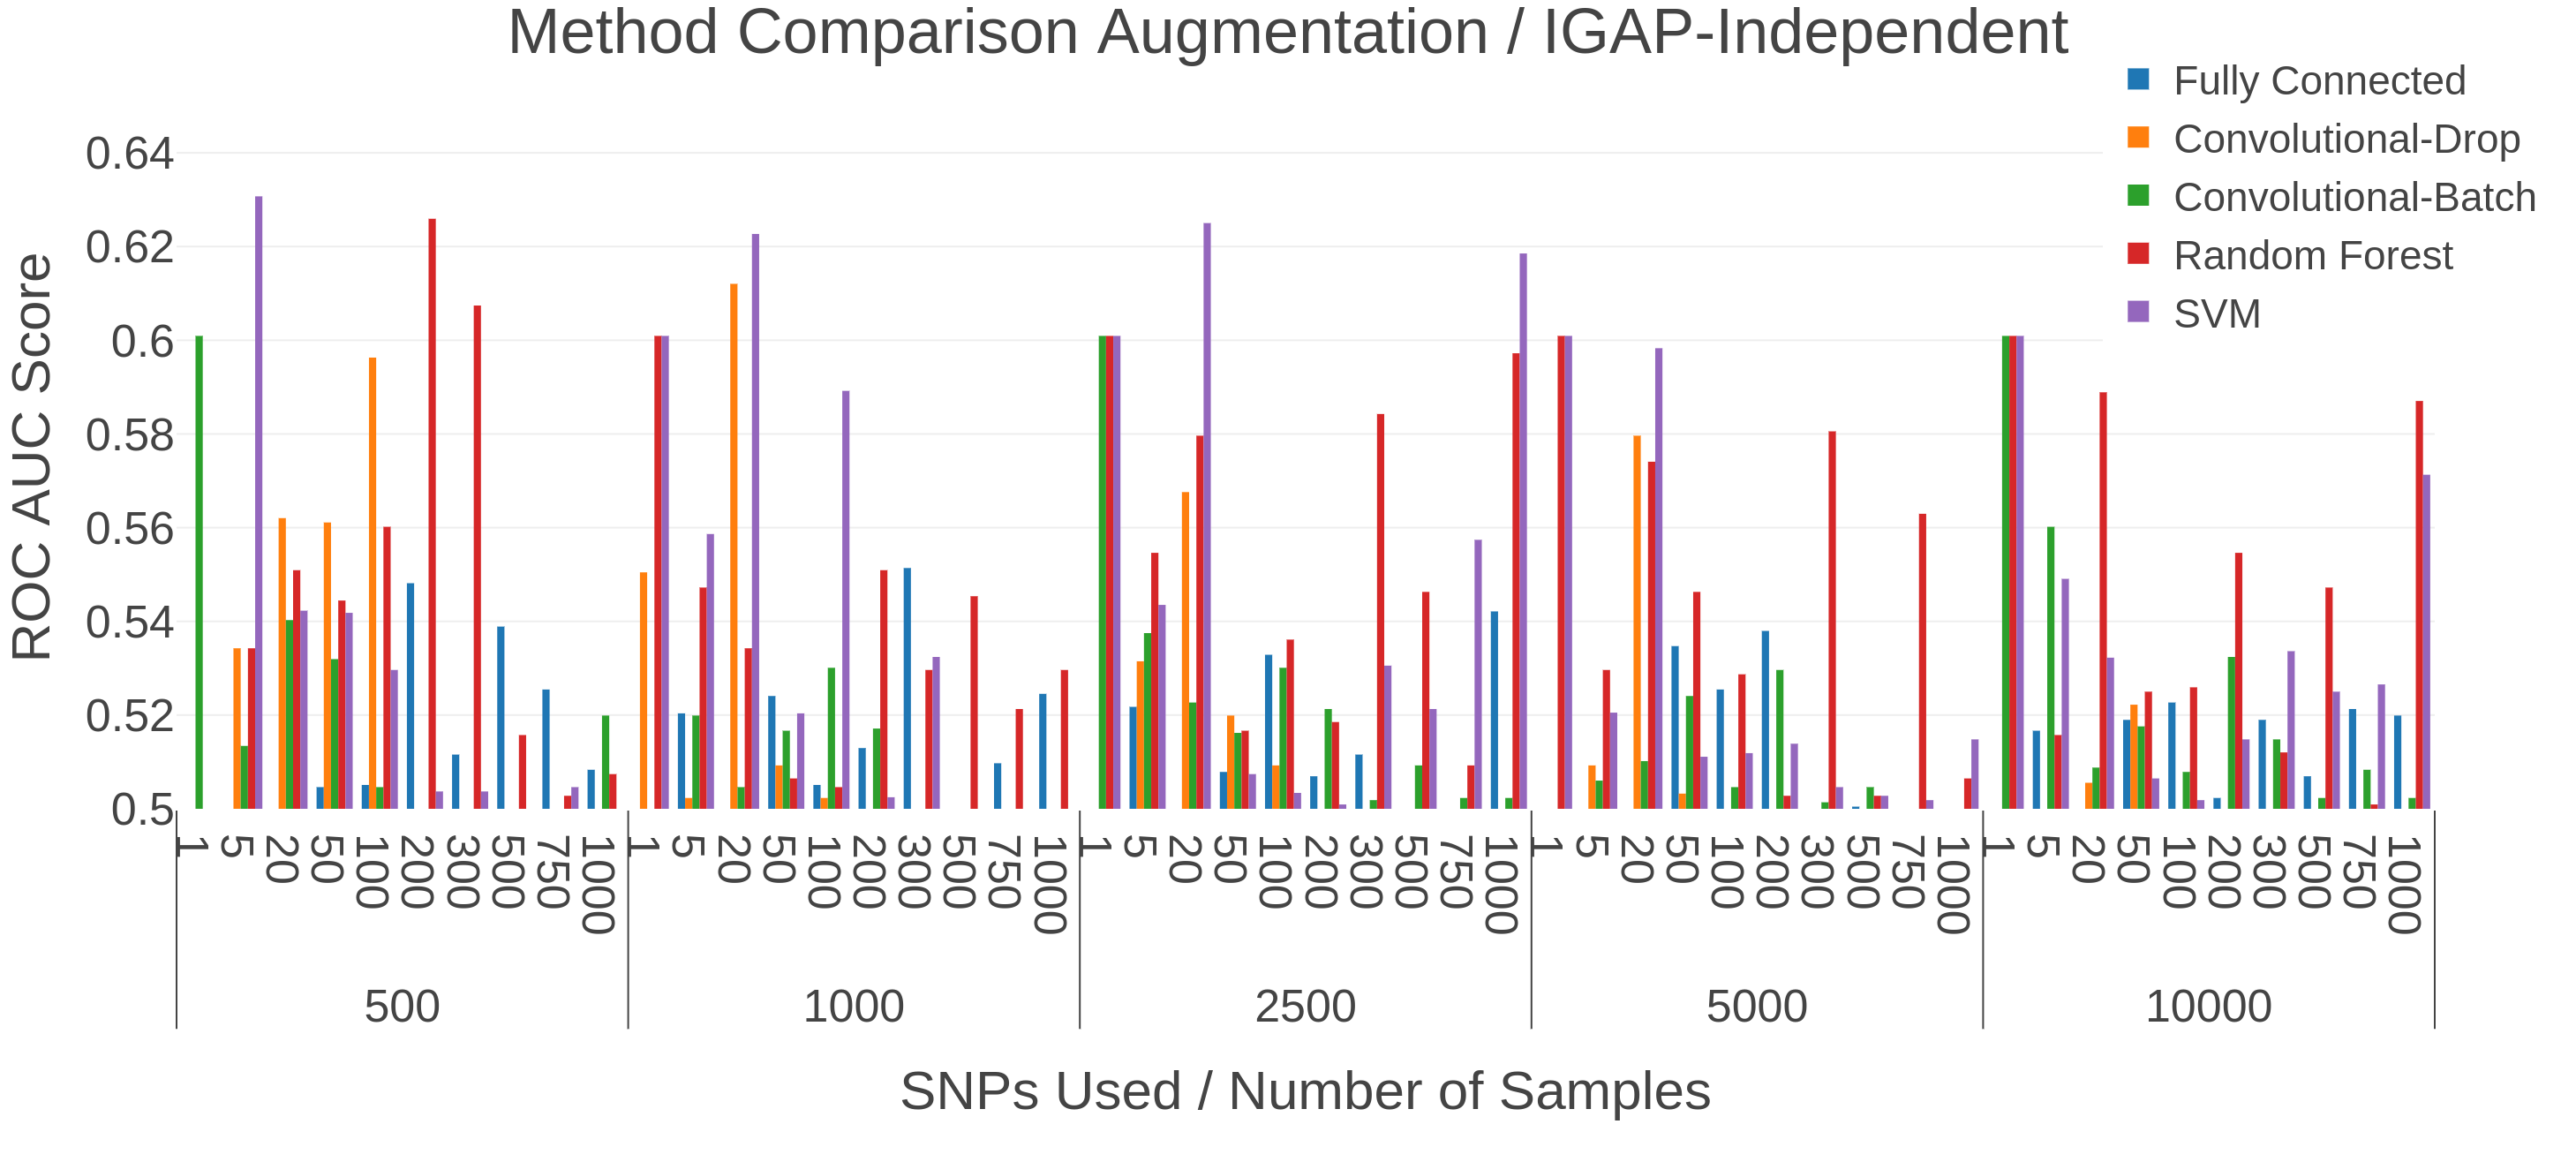
\includegraphics[width=4in]{images/results/DataAugComplete2.png}}
\caption{{\bf Method Comparison with IGAP-Independent Subset}
Comparison between the ROC AUC Score obtained using the different classification methods. The X axis firstly describes an increase of the number of SNPS used for classification, and afterwards an increase in the data-augmentation size validated on the IGAP-Independent subset.}
\label{fig13}
\end{figure}
\newpage
\section{FRESA.CAD}


The first analysis to perform is on the full ADNI dataset using the top 2,500 SNPs. As before, this comes with a caveat, as the full ADNI dataset does include some samples which were present in the IGAP and as such are not completely independent. The results begin by seeing the ROC AUC Score obtained by the different classifiers. Figure 4.11 and 4.12 show this, where it can be seen that the algorithms perform in the order of 0.60\~0.70. BSIWMS, LASSO and RPART show the best results in this case, and definitely the ensemble of the methods is the one with the best performance, achieving a ROC score of 0.719. Thus it can be seen how the use of the ensemble of methods appears to give the best results for the full dataset case, and they appear to outdo the previous methods. 

 \begin{figure}[!ht]
\centerline{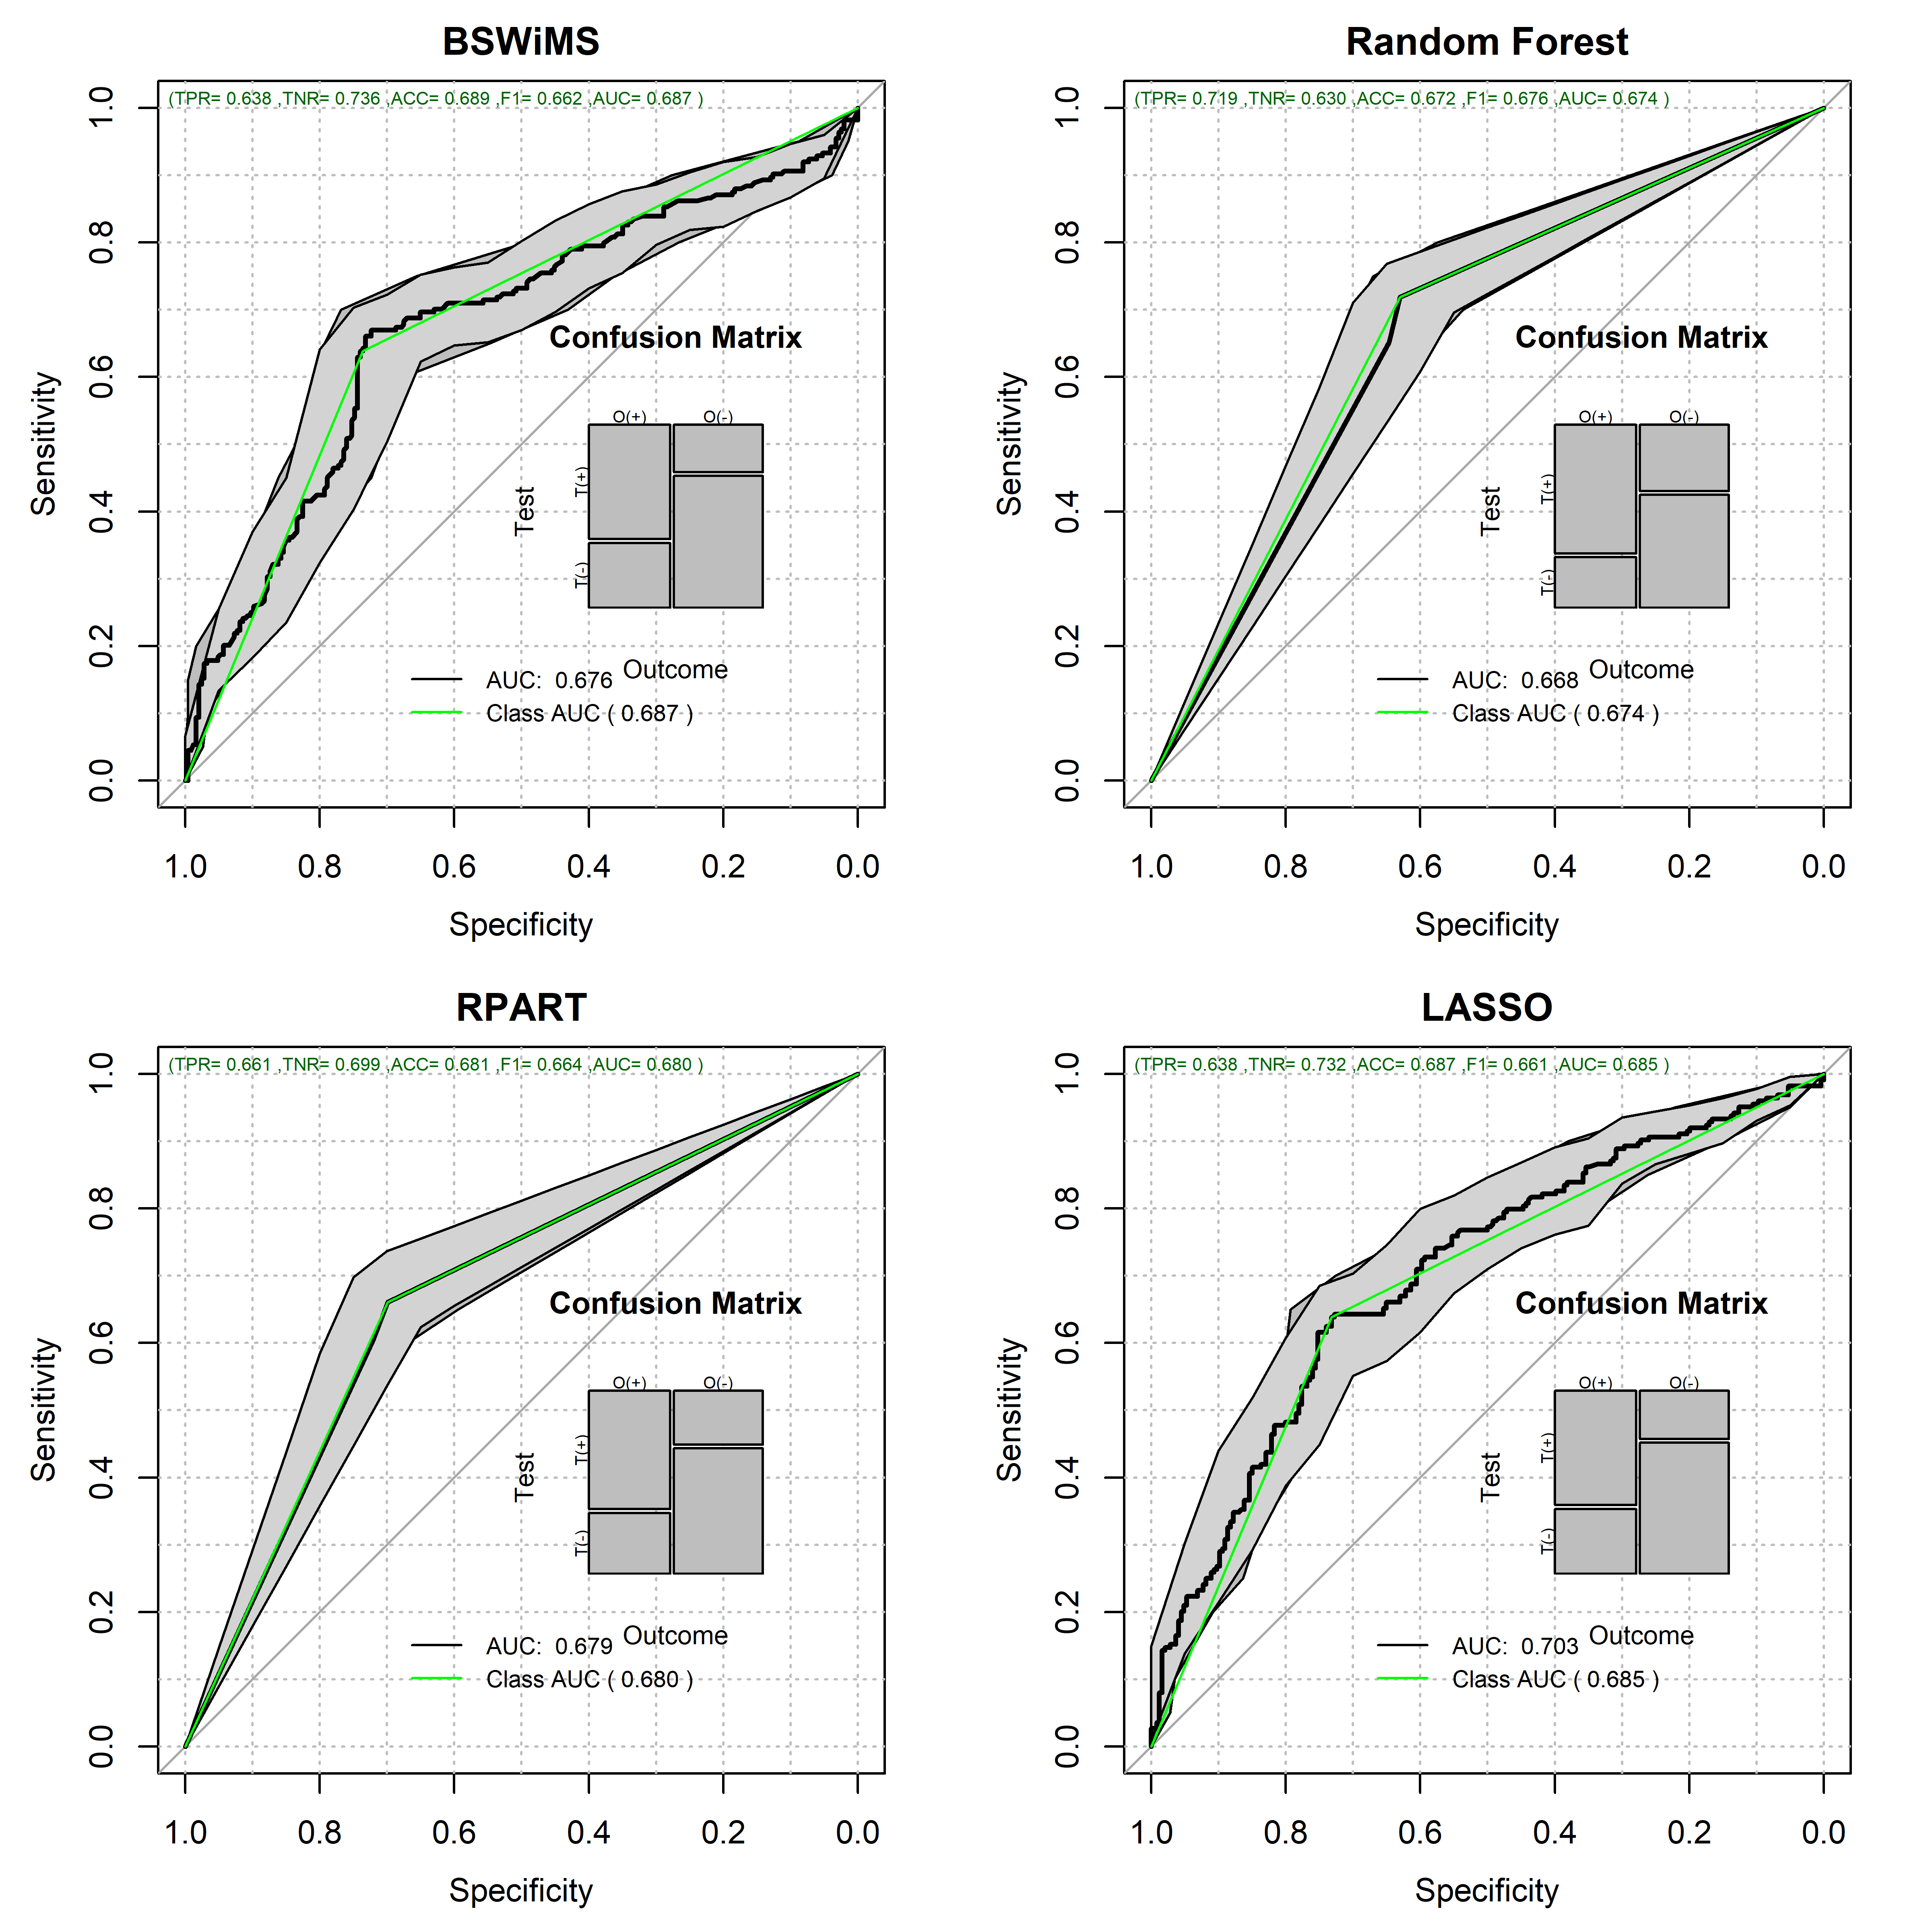
\includegraphics[width=3in]{images/results/fresaCurves1.png}}
\caption{{\bf ROC Curves for the FRESA.CAD Benchmarking Classifiers} 
ROC Curves obtained using BSWiMS, Random Forest, RPART and LASSO of the FRESA.CAD Benchmarking with the complete ADNI dataset for the Cross-Validation and the top 2,500 SNPs as inputs}
\label{fig14}
\end{figure}

 \begin{figure}[!ht]
\centerline{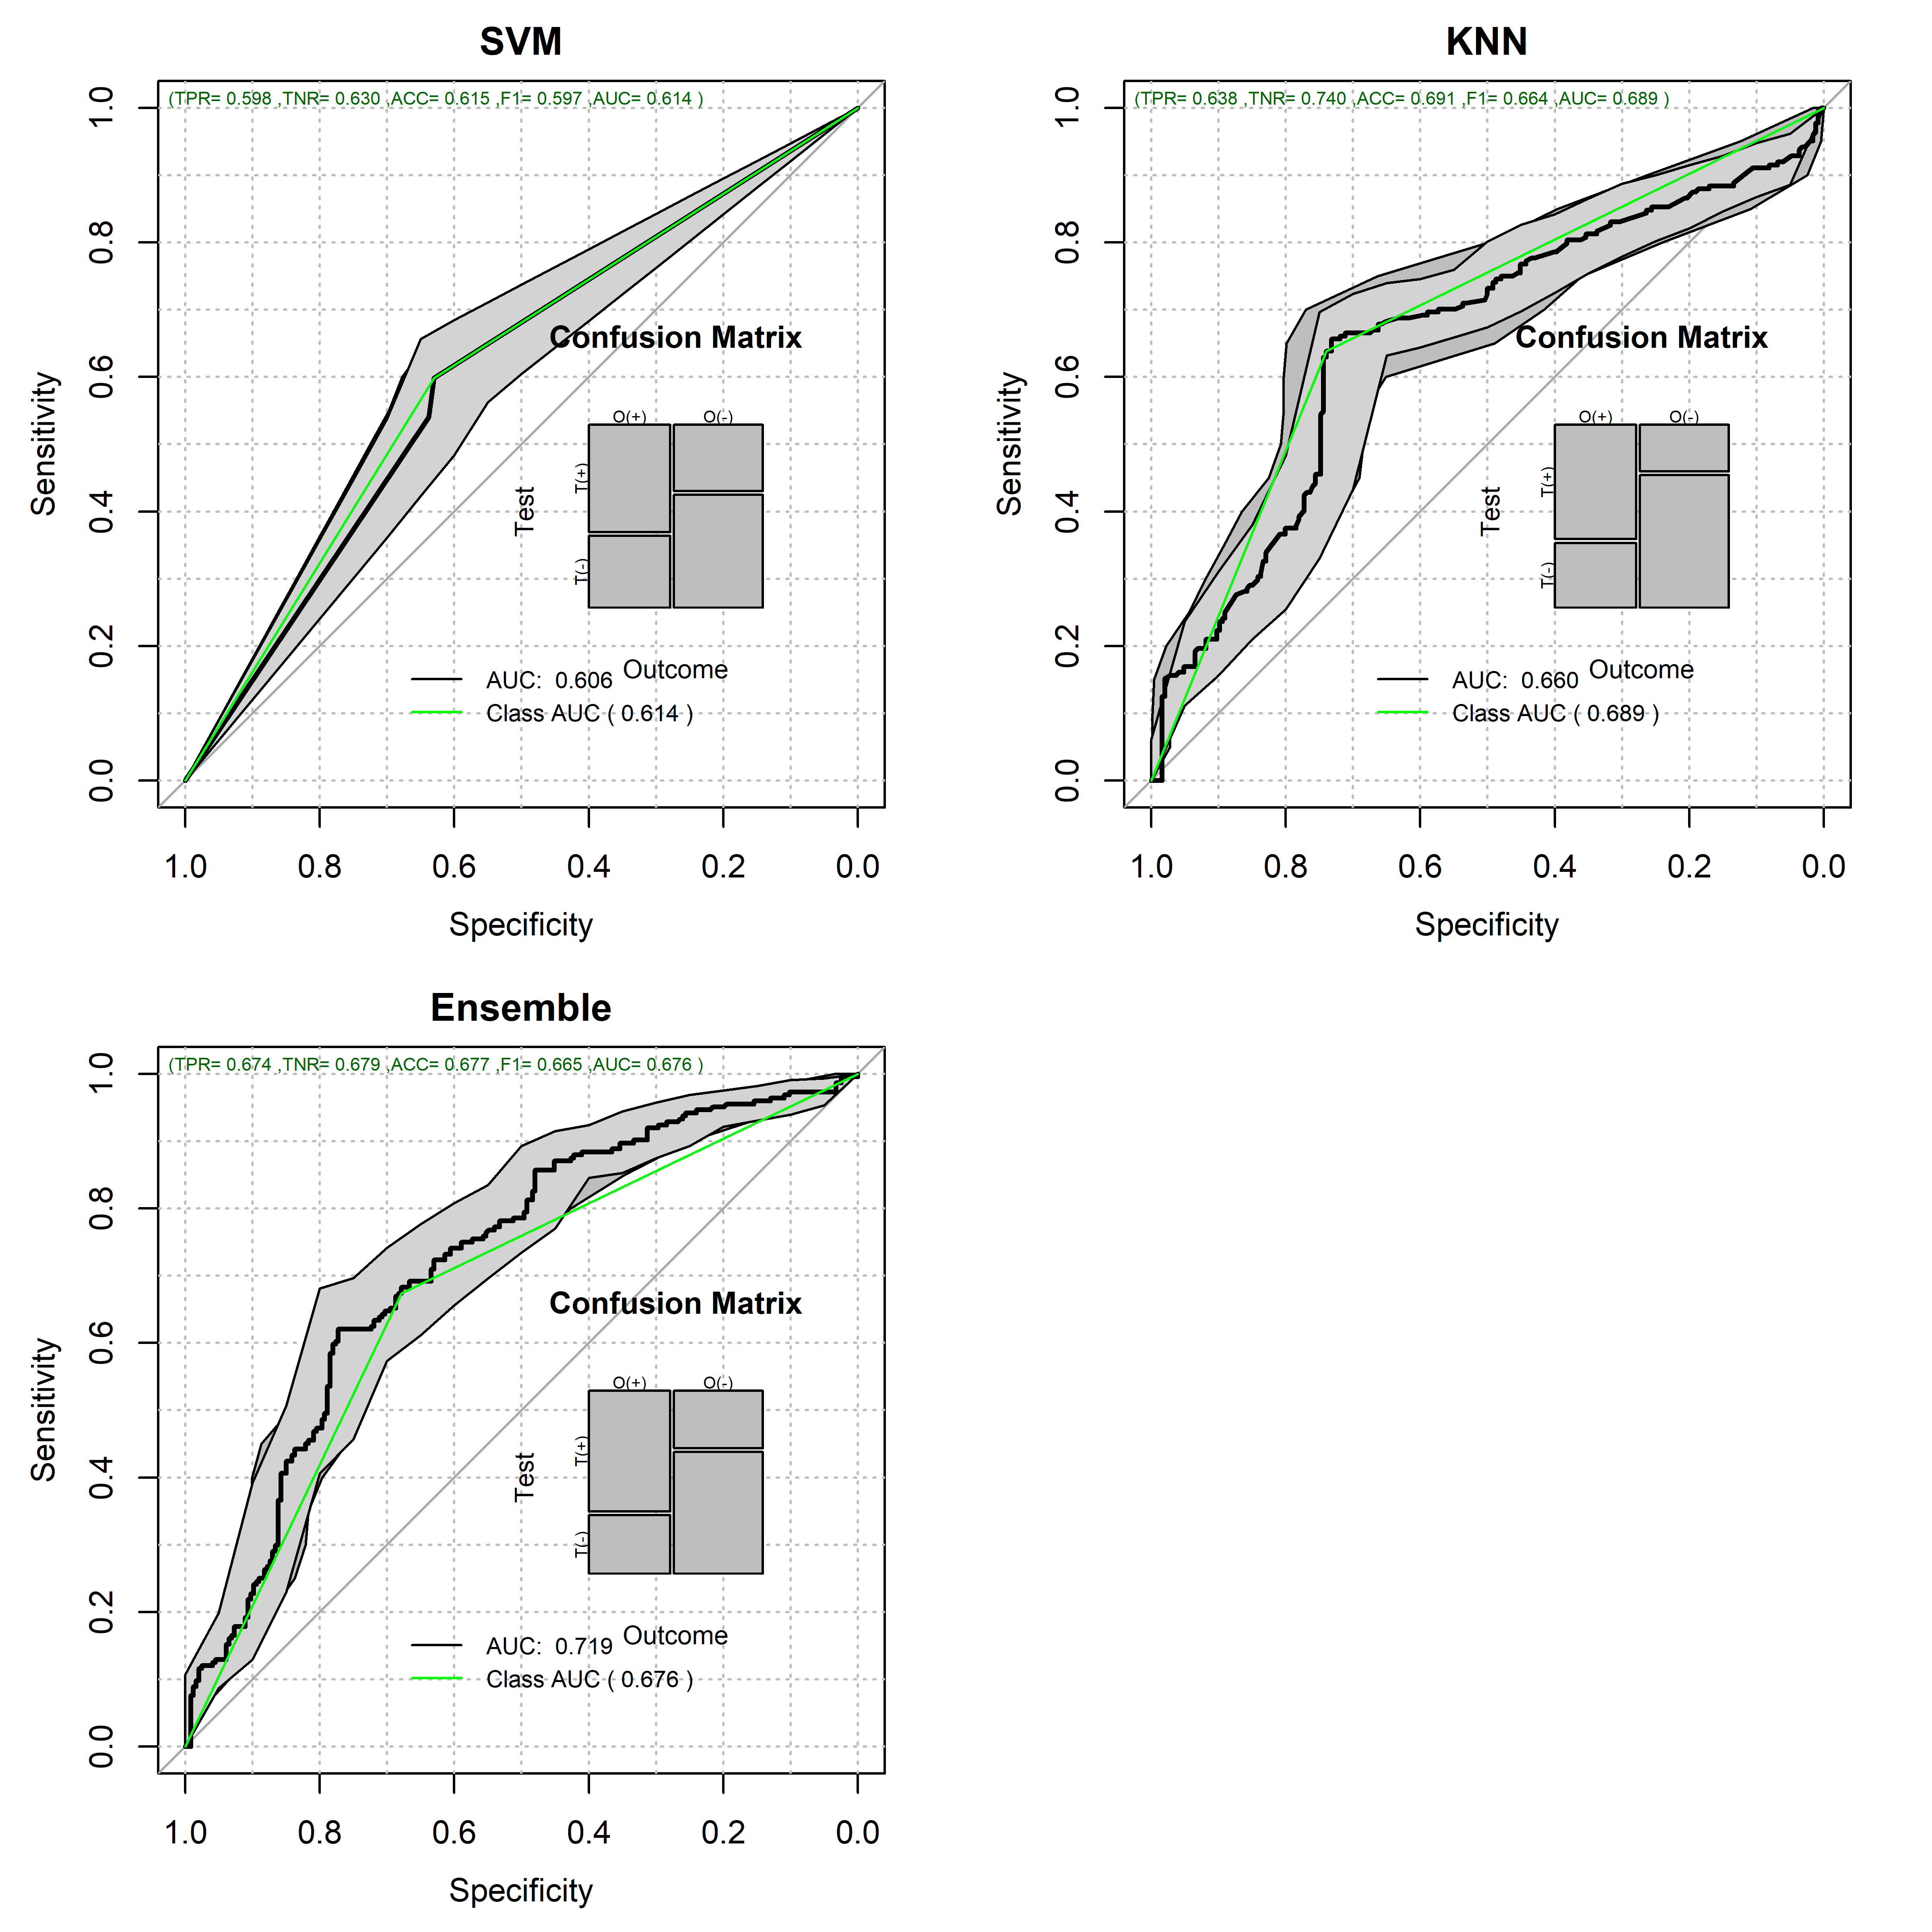
\includegraphics[width=3in]{images/results/fresaCurves2.png}}
\caption{{\bf ROC Curves for the FRESA.CAD Benchmarking Classifiers (Continued)} 
ROC Curves obtained using SVM, KNN and the Ensemble of the FRESA.CAD Benchmarking with the complete ADNI dataset for the Cross-Validation and the top 2,500 SNPs as inputs}
\label{fig141}
\end{figure}

The first characteristic to analyze with the benchmark is the similarity of classifiers across the classification. In figure 4.13 this is shown, and it can be observed that for cases and controls the values seem to be evenly classified for all SVMs, which means they are learning roughly the same variables and results. In the case of the LASSO it appears to be having trouble with some samples where there is not a clear difference (This can be seen in the Ensemble in a smaller manner). These methods are not entirely certain an individual belongs to either category. BSWIMS and KNN do classify some cases very strongly, but then do not perform that well in some other cases (Which could be due to selecting few features). The ensemble obtains a point in between these two groups which can be seen in the final results. In general it can be seen that in general the algorithms misclassify almost all of the same samples either for cases or for controls (Except the SVM with mRMR feature selection) and as such could give an idea of samples that either share characteristics that make them hard to classify, there is not enough information to further classify the problem or that they could be samples that could become cases in the future.
 
 \begin{figure}[!ht]
\centerline{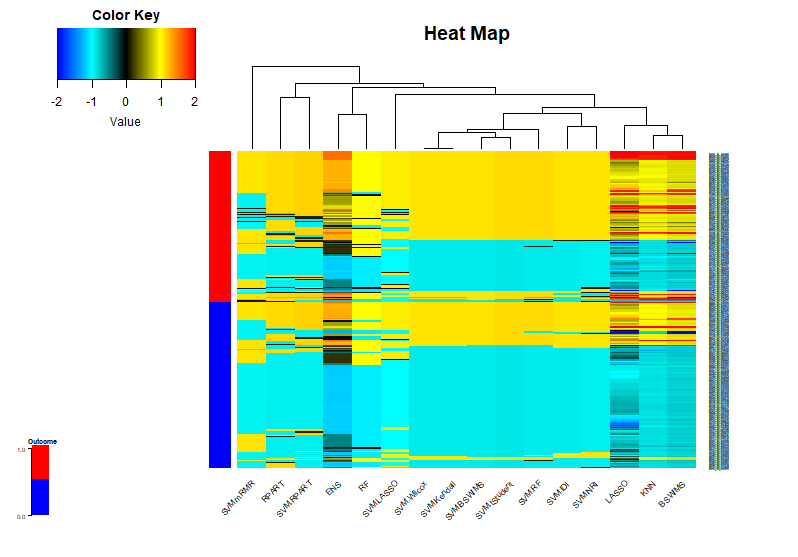
\includegraphics[width=3in]{images/results/fresaHM.png}}
\caption{{\bf Heatmap prediction comparison between FRESA.CAD Benchmark classifiers} 
Heatmap comparison of the prediction performance across classifiers. The Y axis describes each sample of the dataset with the real value (colour bar on the left) as well as the predicted value, while the X axis describes the different classifiers of the FRESA.CAD Benchmarking with the complete ADNI dataset for the Cross-validation and using the top 2,500 SNPs as input}
\label{fig15}
\end{figure}



In Figure 4.14 the Jaccard index is shown on the left; that is, the similarity between classifiers according to the features selected by each. In the dataset it can be observed that the BSWIMS has a high Jaccard Index and shows that the few features selected in that model are shared in more models. This makes sense as BSWiMS is choosing the APOE $\epsilon4$ gene as the main indicator, which has a high prediction power compared to all others and they do tend to choose it. As shown, an increase in the number of features (Right side of the figure) means that the Jaccard index starts to go lower as is the case for LASSO and RPART which are some of the best performers. The number of SNPs for these two models ranges from 30 to 75 SNPs, and as such it would seem using a higher number of SNPs could add additional information, although other models do use lower number of SNPs with good precision. There exists a balance that could show a number of variants in the range of decades is the best solution.

\begin{figure}[!ht]
\centerline{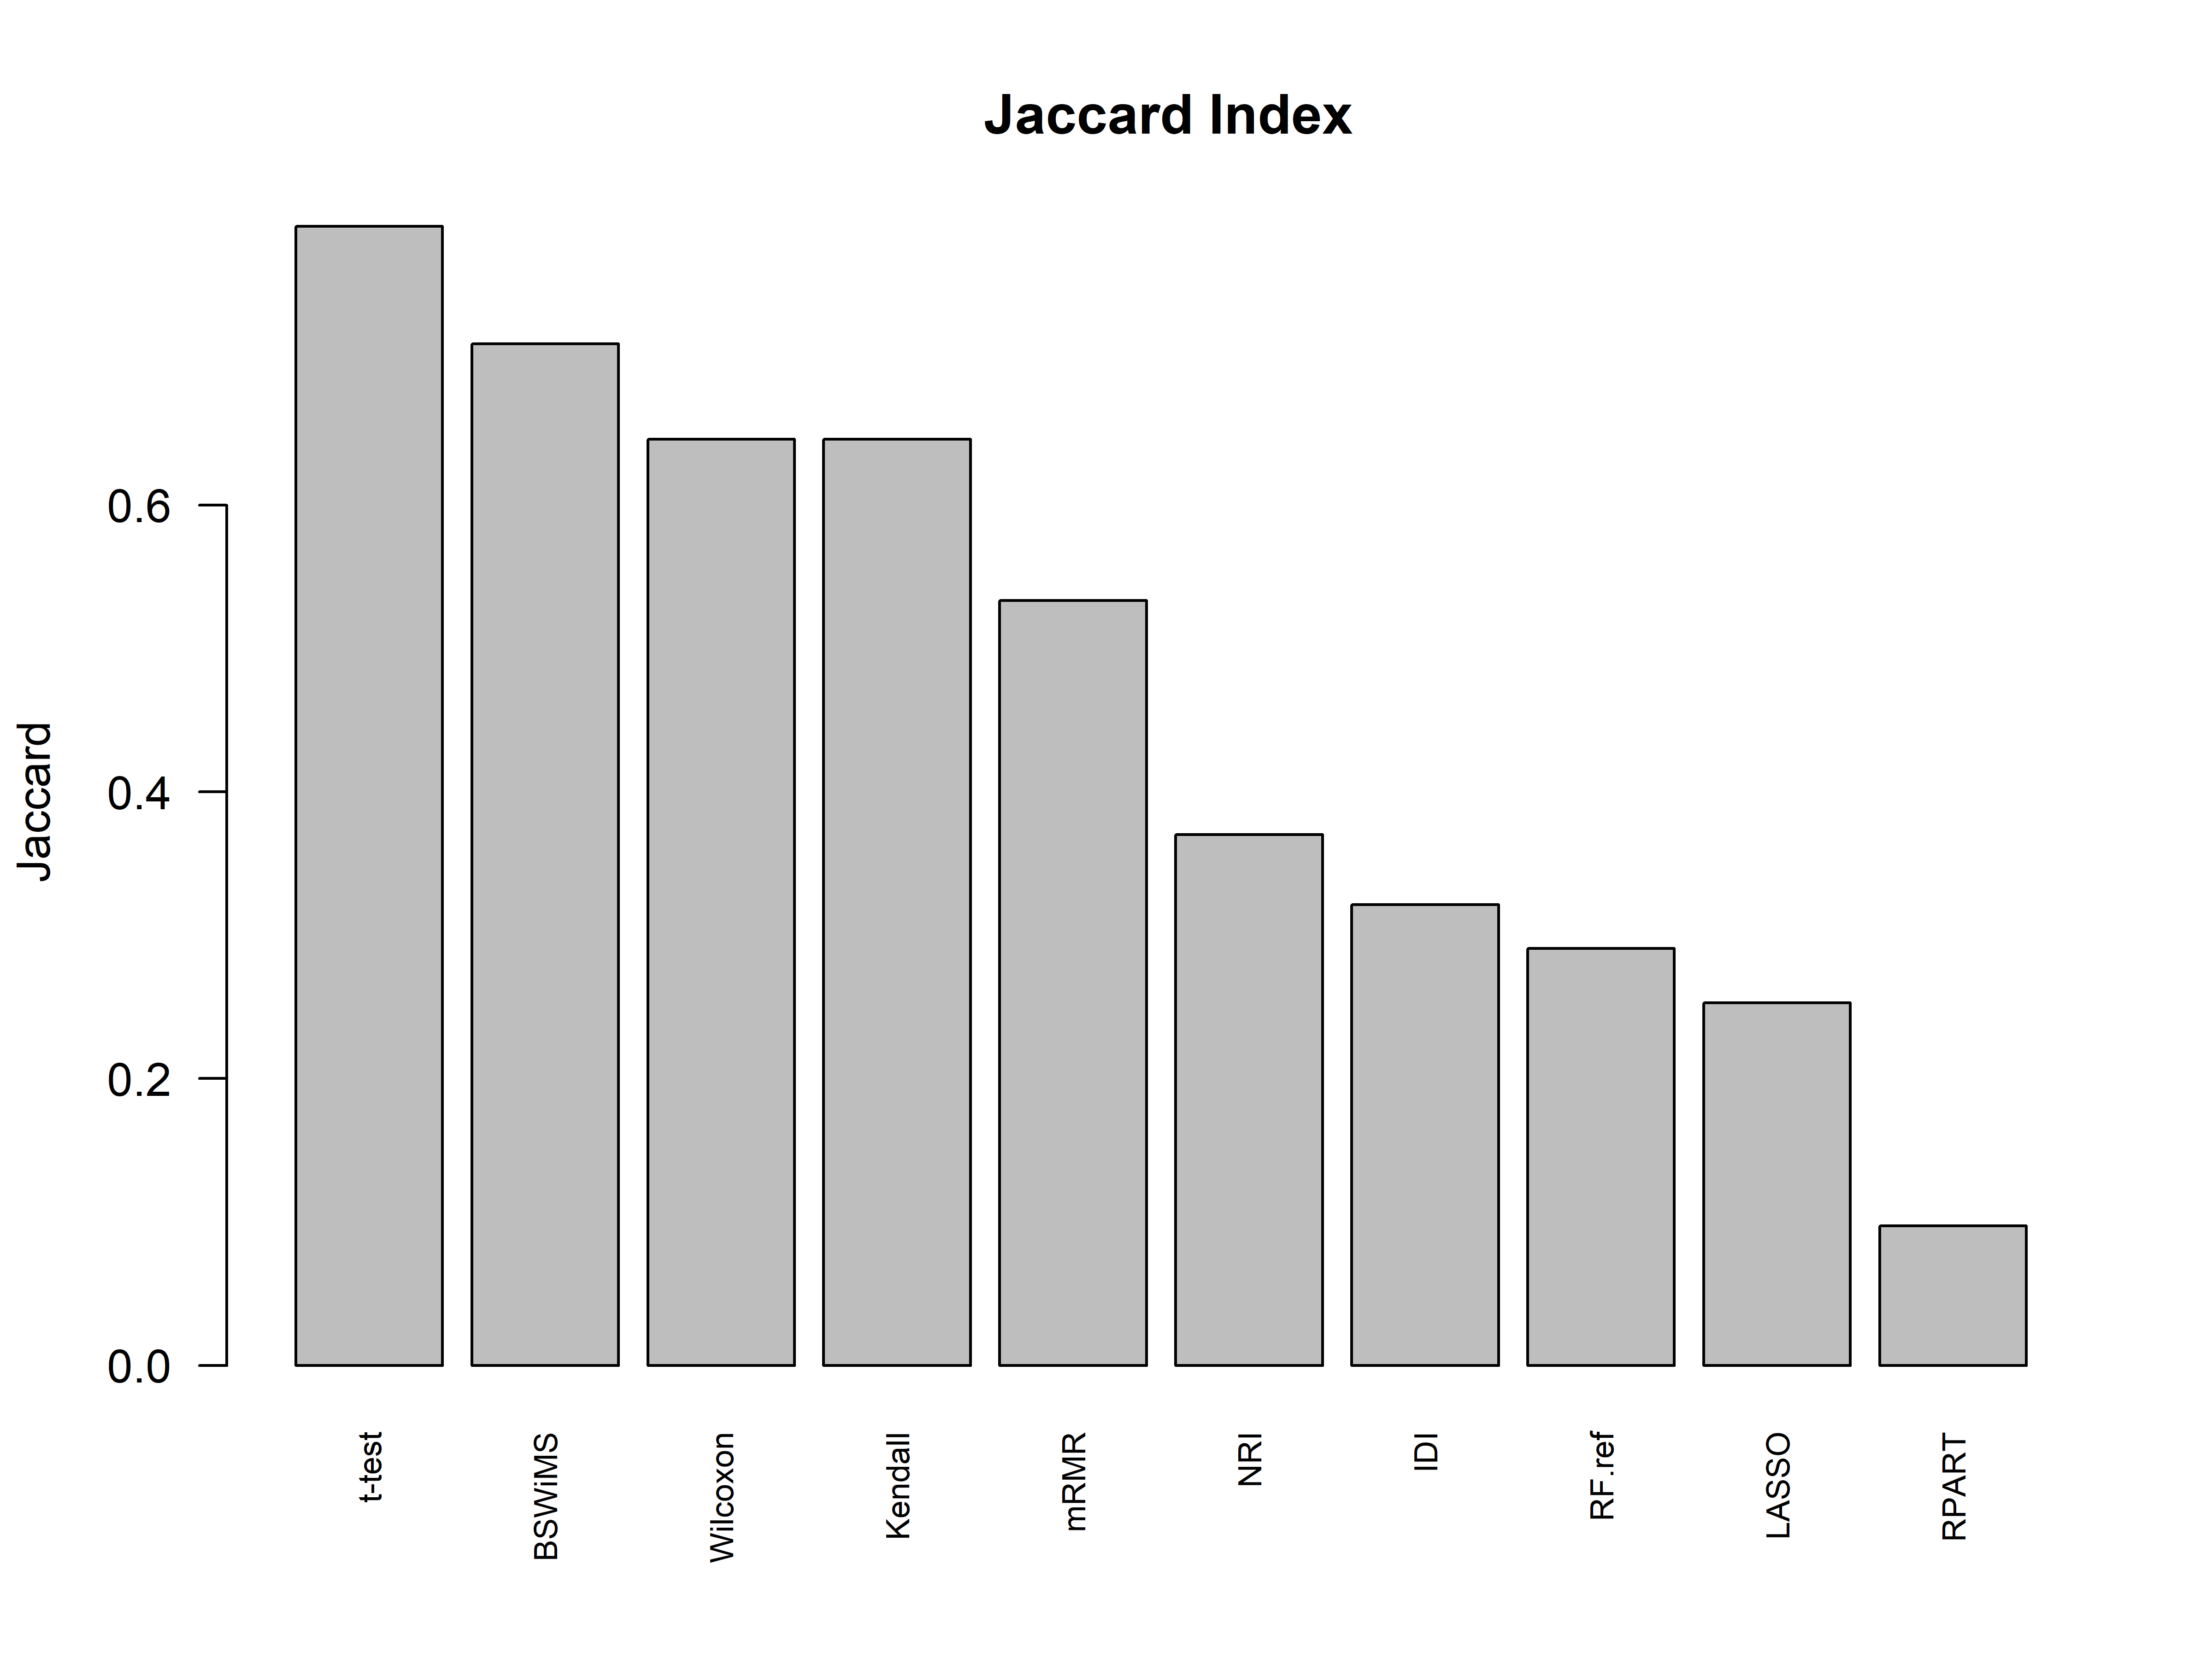
\includegraphics[width=2in]{images/results/fresaJac.png}}
\centerline{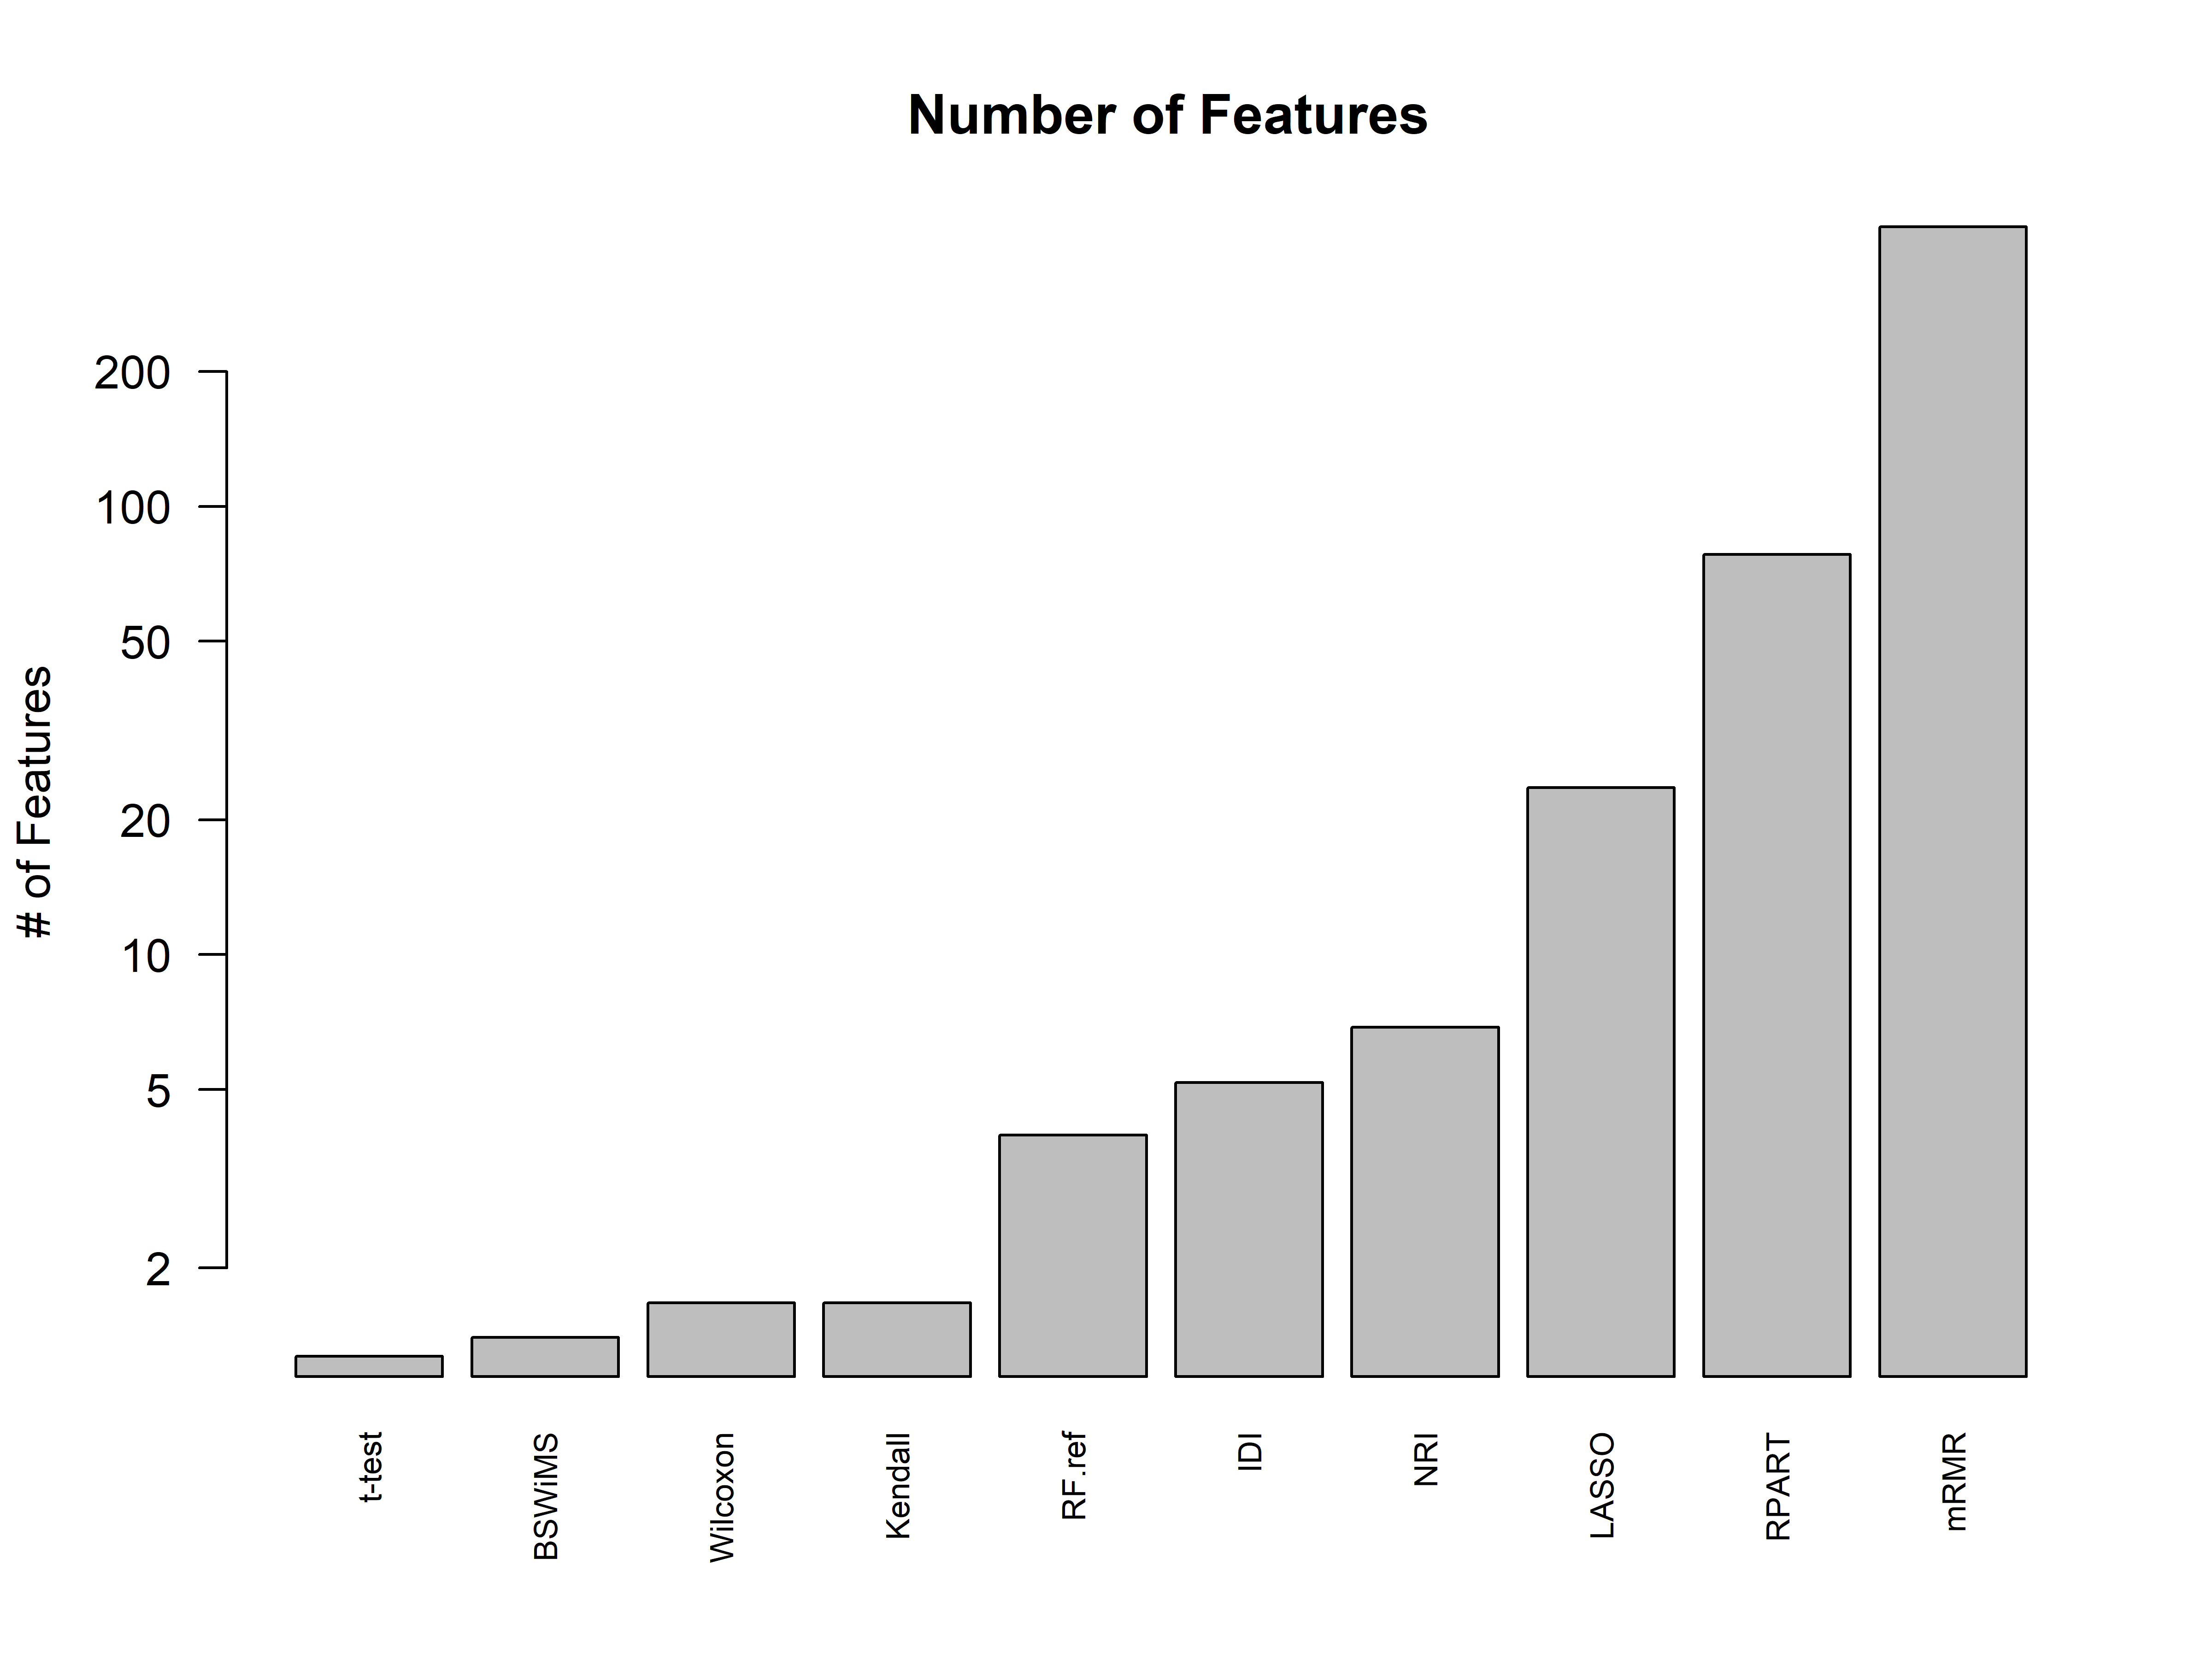
\includegraphics[width=2in]{images/results/fresaFeatures.png}}
\caption{{\bf Jaccard Index and Number of Features} 
Jaccard Index metric of the different classifiers between features selected as well as the number of features selected by each classifier of the FRESA.CAD Benchmarking with the complete ADNI dataset for the Cross-validation and using the top 2,500 SNPs as input }
\label{fig16}
\end{figure}
\newpage
With Figure 4.15 and 4.16 the analysis can be further expanded to see the balanced Error, AUC, Accuracy as well as Specificity and Sensitivity for both classifiers and the combinations with filters. As expected, BSWiMS performs quite well in the Balanced Error and the other metrics, then the ensemble, while RPART and LASSO perform slightly worse. In the filters the Random Forest filter gives the best results for the ROC, while some other filters such as Spearman or KNN perform well in just one of the two cases, as such it might be better to use certain combinations depending on the importance of detecting a case or a control more precisely. And thanks to the confidence intervals given it can be seen that only SVMs would perform worse than the others. This supports the idea seen in the heatmap analysis.
\clearpage
 \begin{figure}[!ht]
\centerline{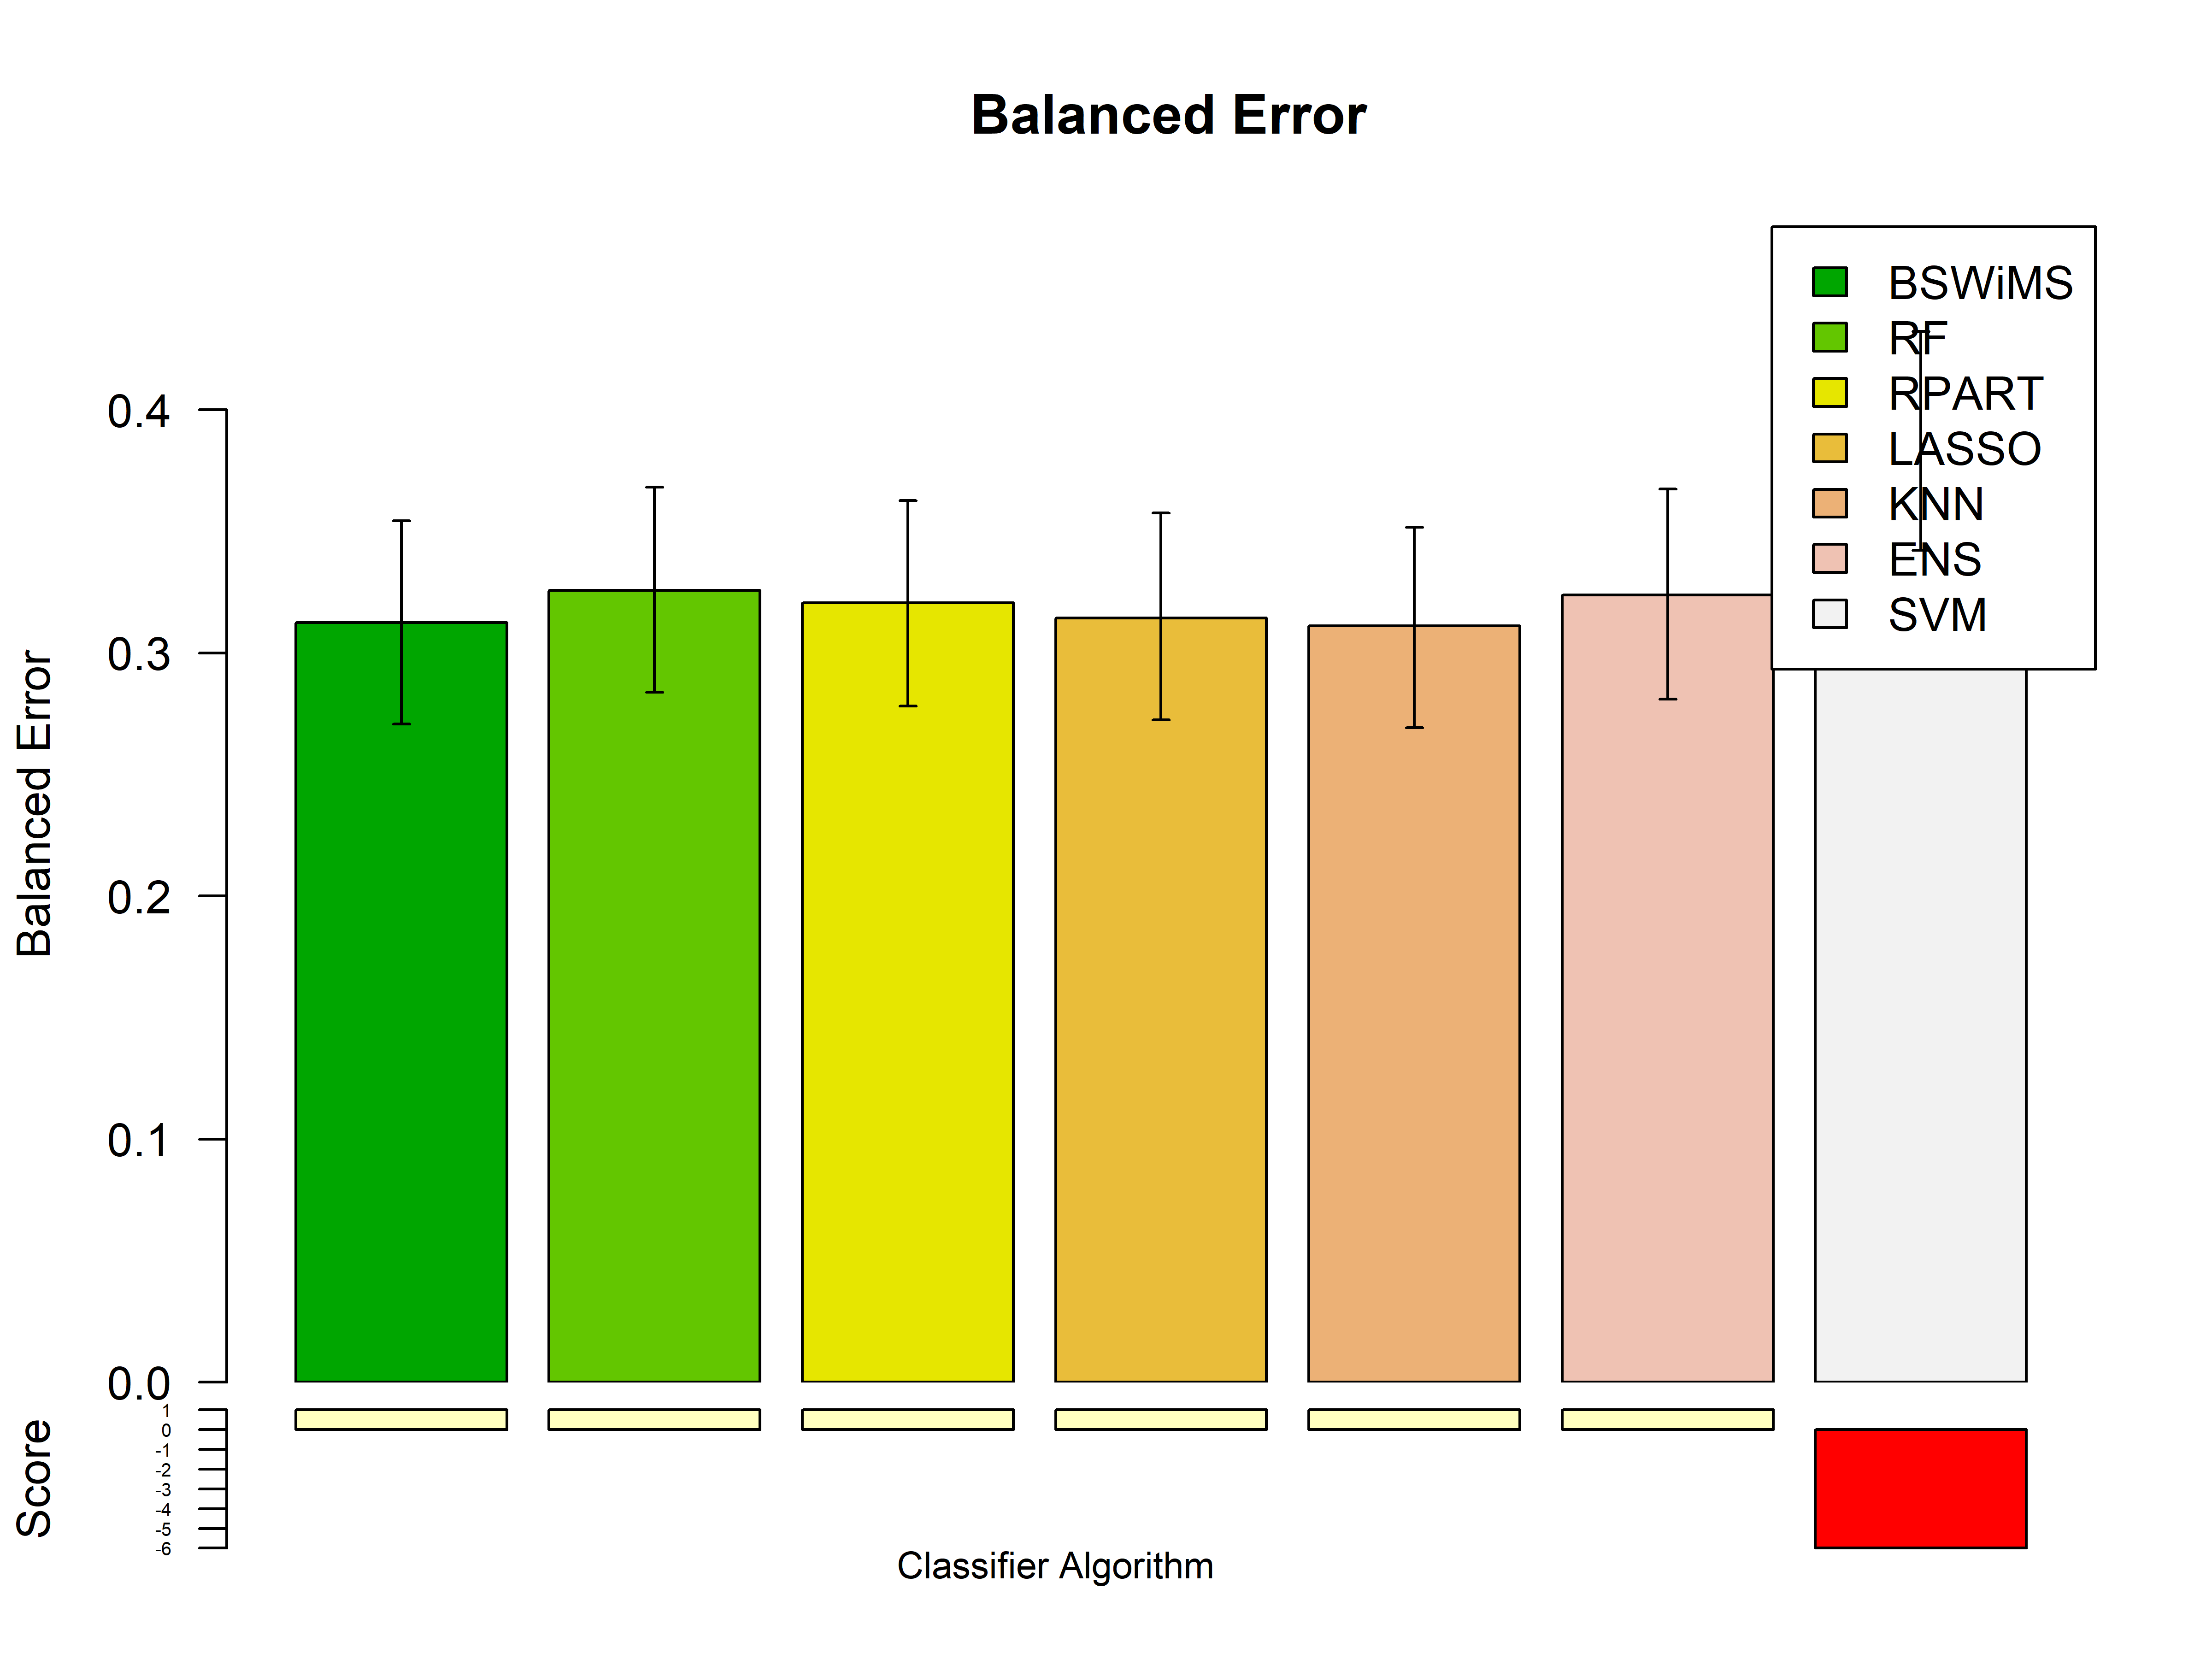
\includegraphics[width=5in,height=2in]{images/results/fresaBE.png}}
\centerline{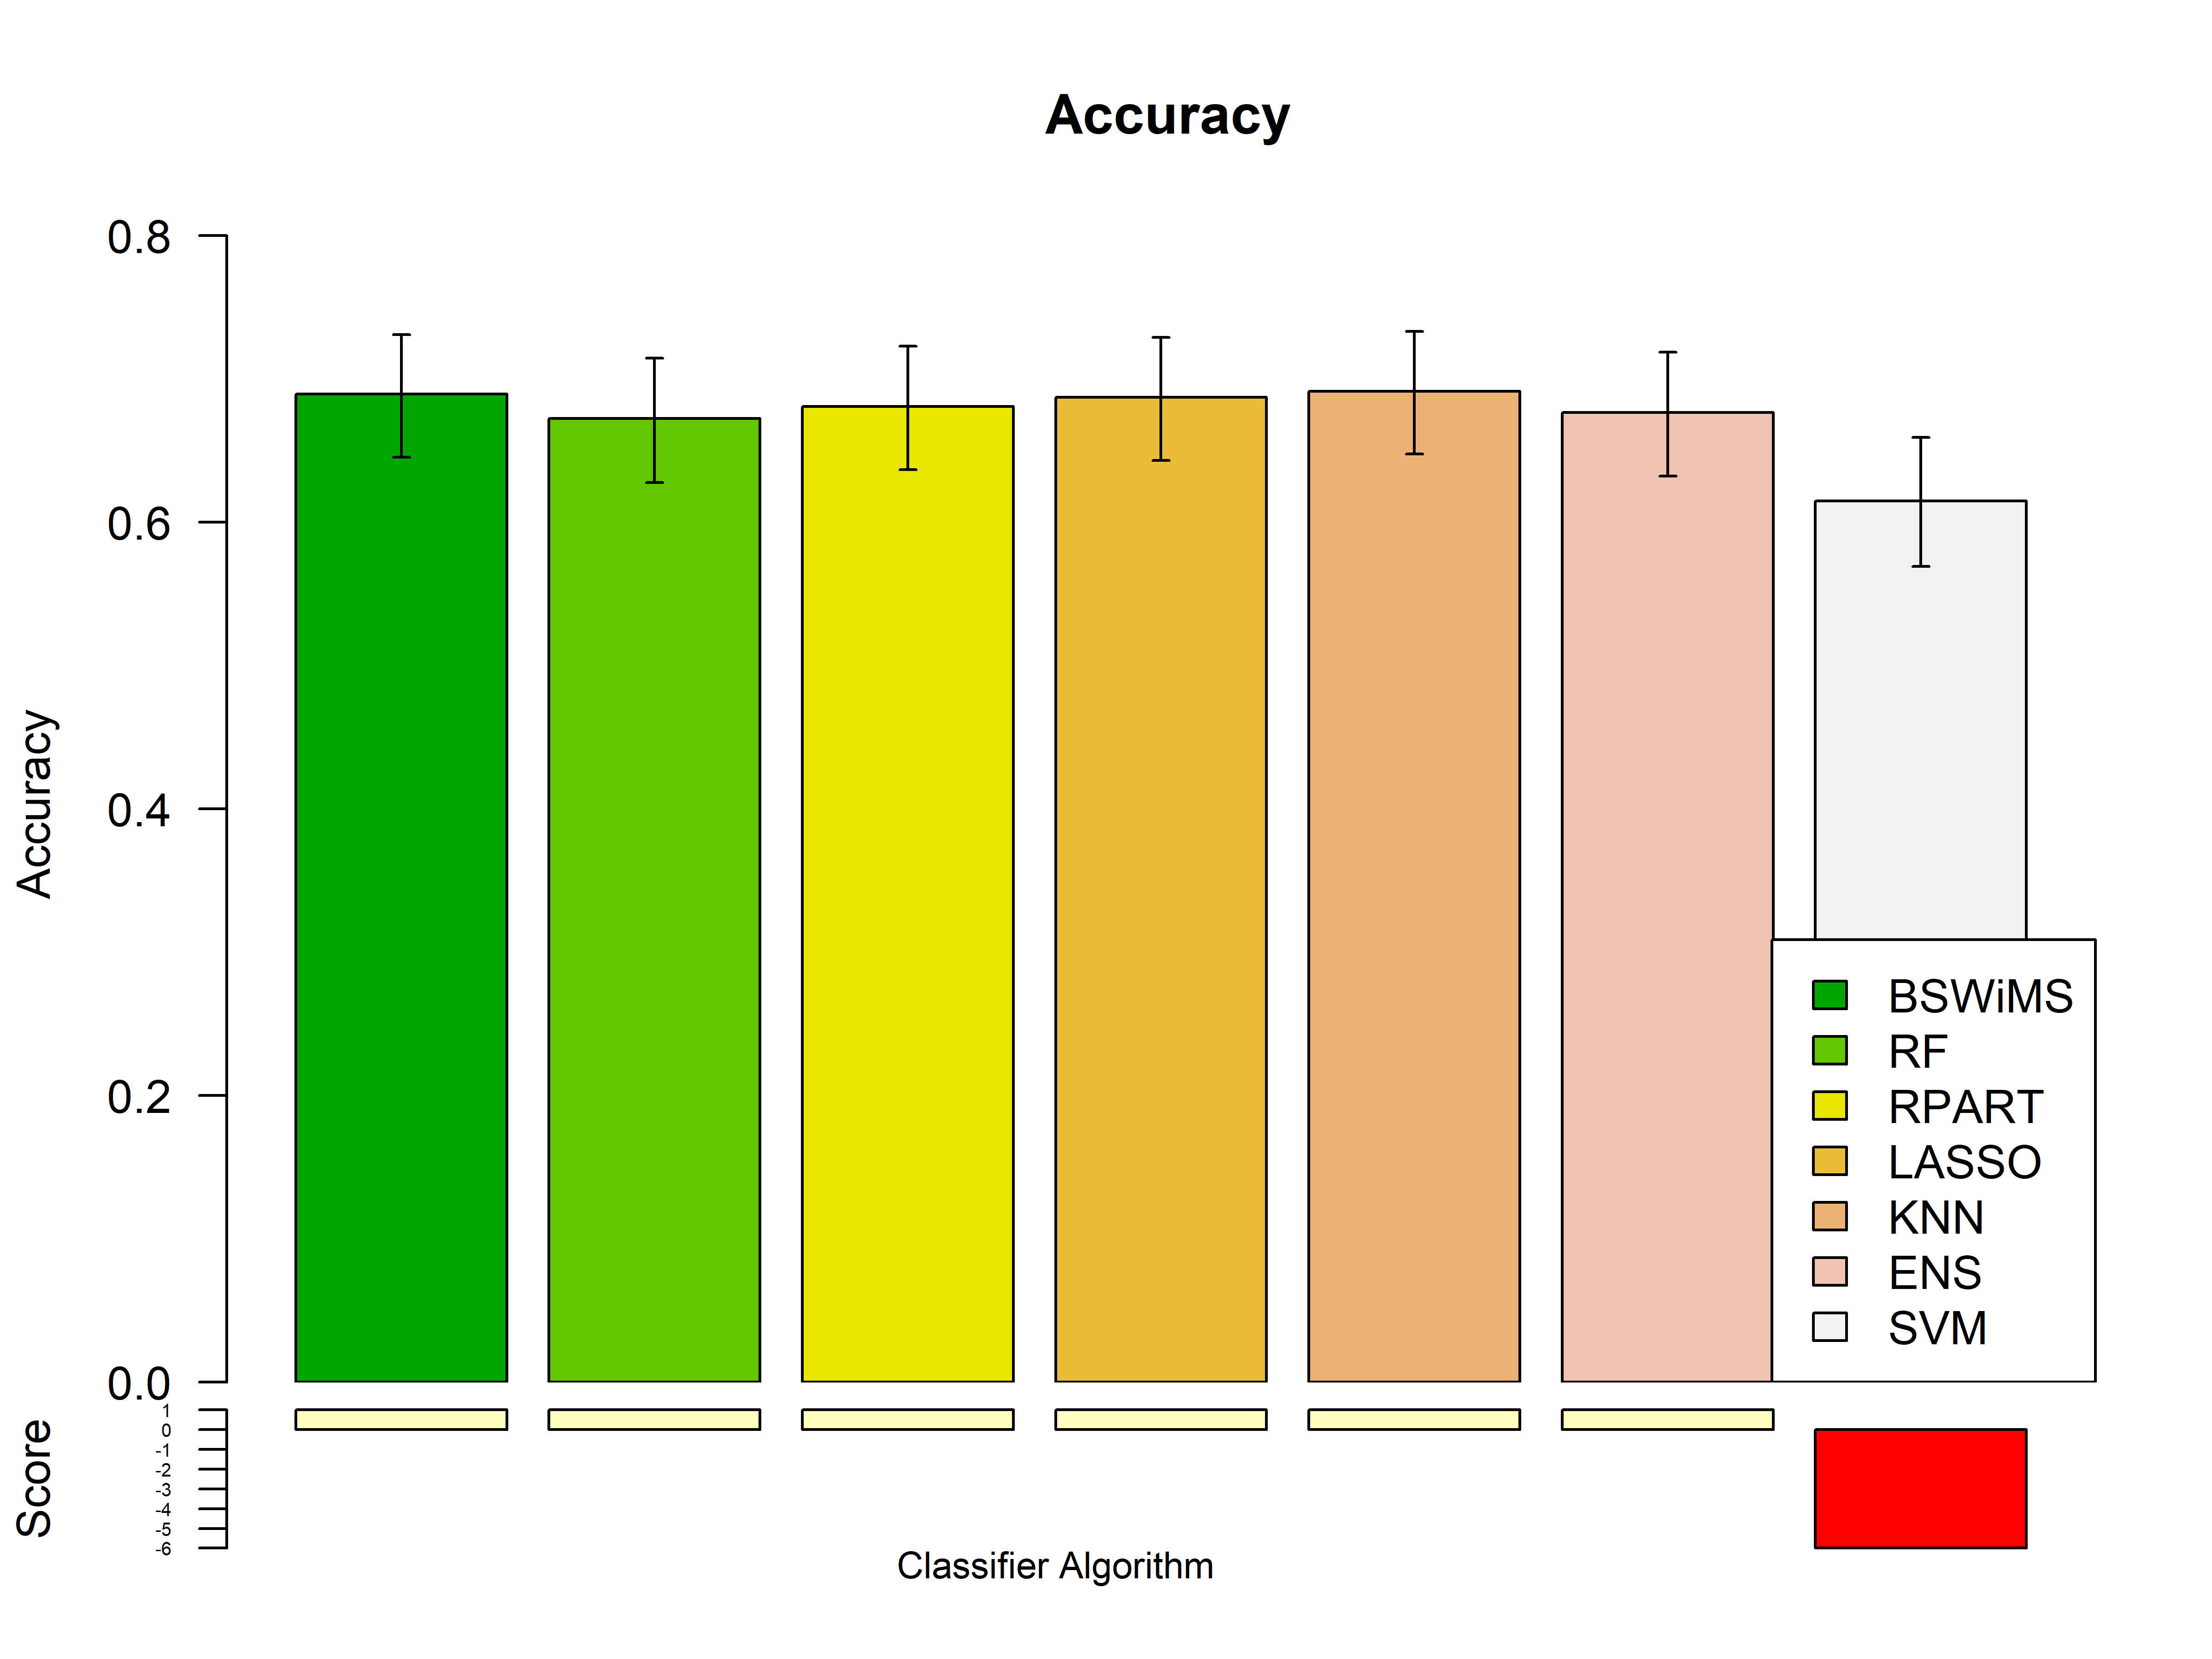
\includegraphics[width=5in,height=2in]{images/results/fresaAcc.png}}
\centerline{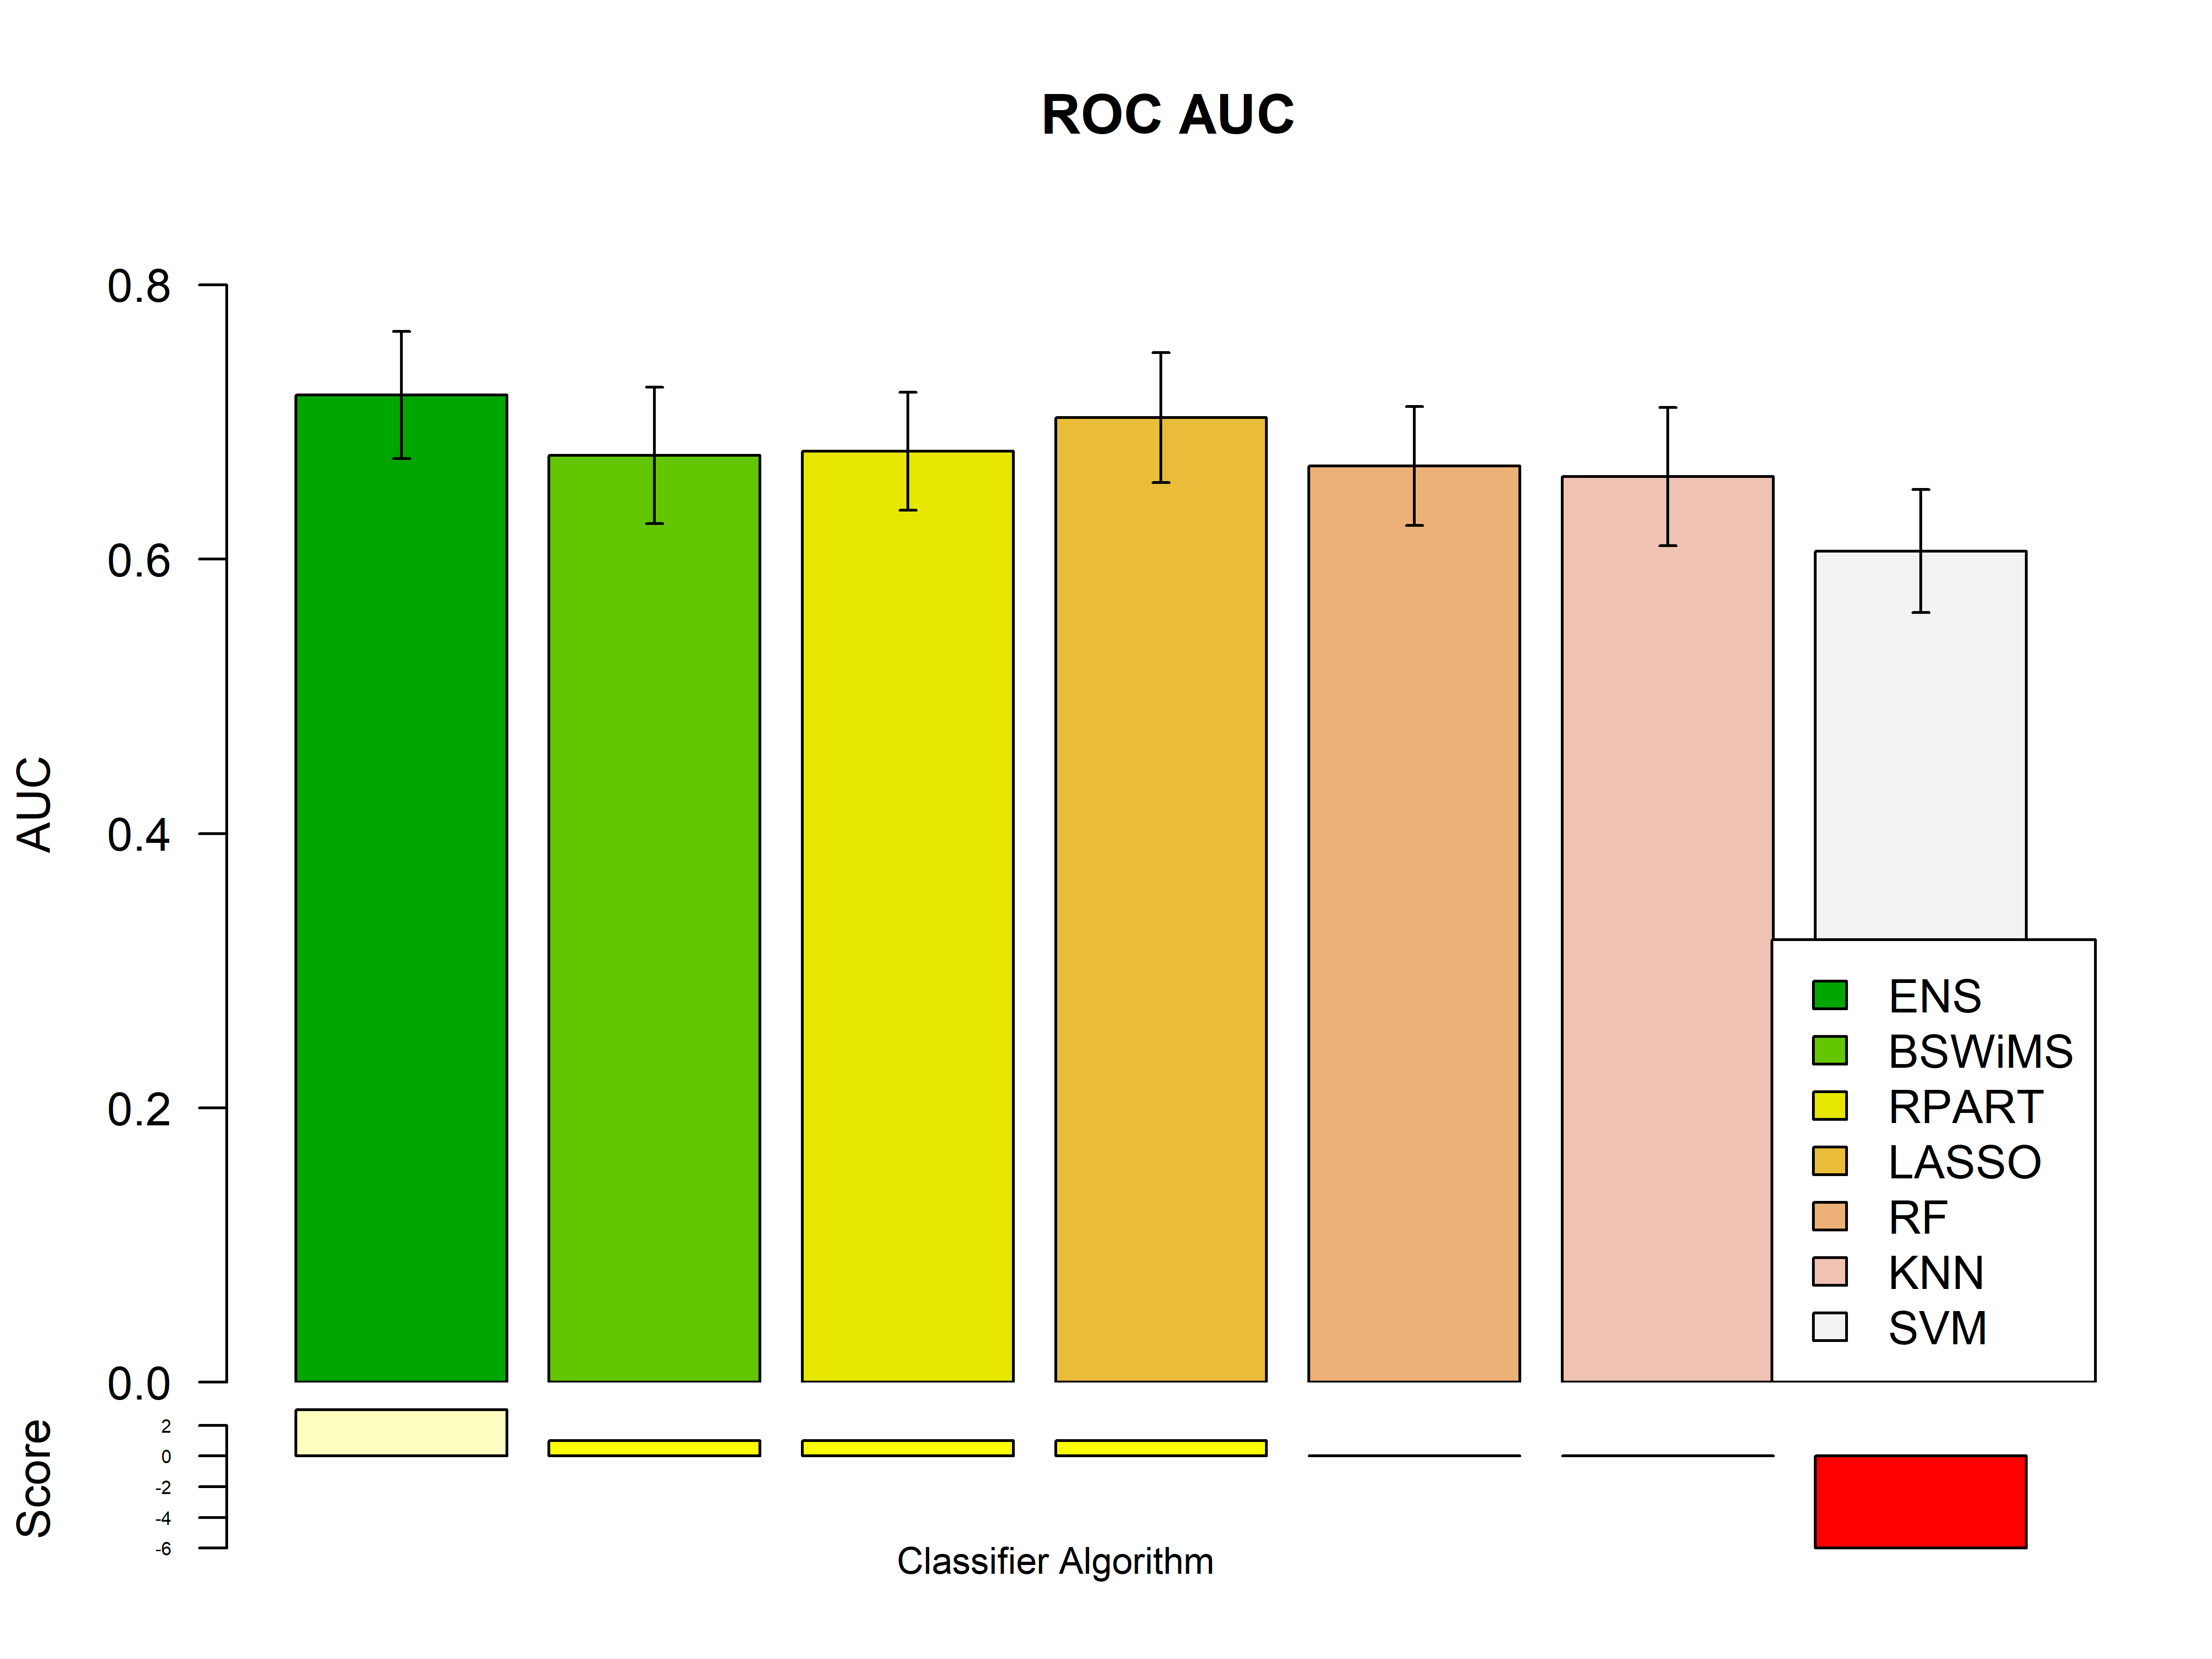
\includegraphics[width=5in,height=2in]{images/results/fresaAUC.png}}
\caption{{\bf Balanced Error, Accuracy and AUC of the FRESA.CAD Benchmark classifiers} 
Comparison between the Balanced Error, Accuracy and AUC Score obtained using the different classification methods of the FRESA.CAD Benchmarking with the complete ADNI dataset for the Cross-validation and using the top 2,500 SNPs as input}
\label{fig17}
\end{figure}

   
\begin{figure}[!ht]
\centerline{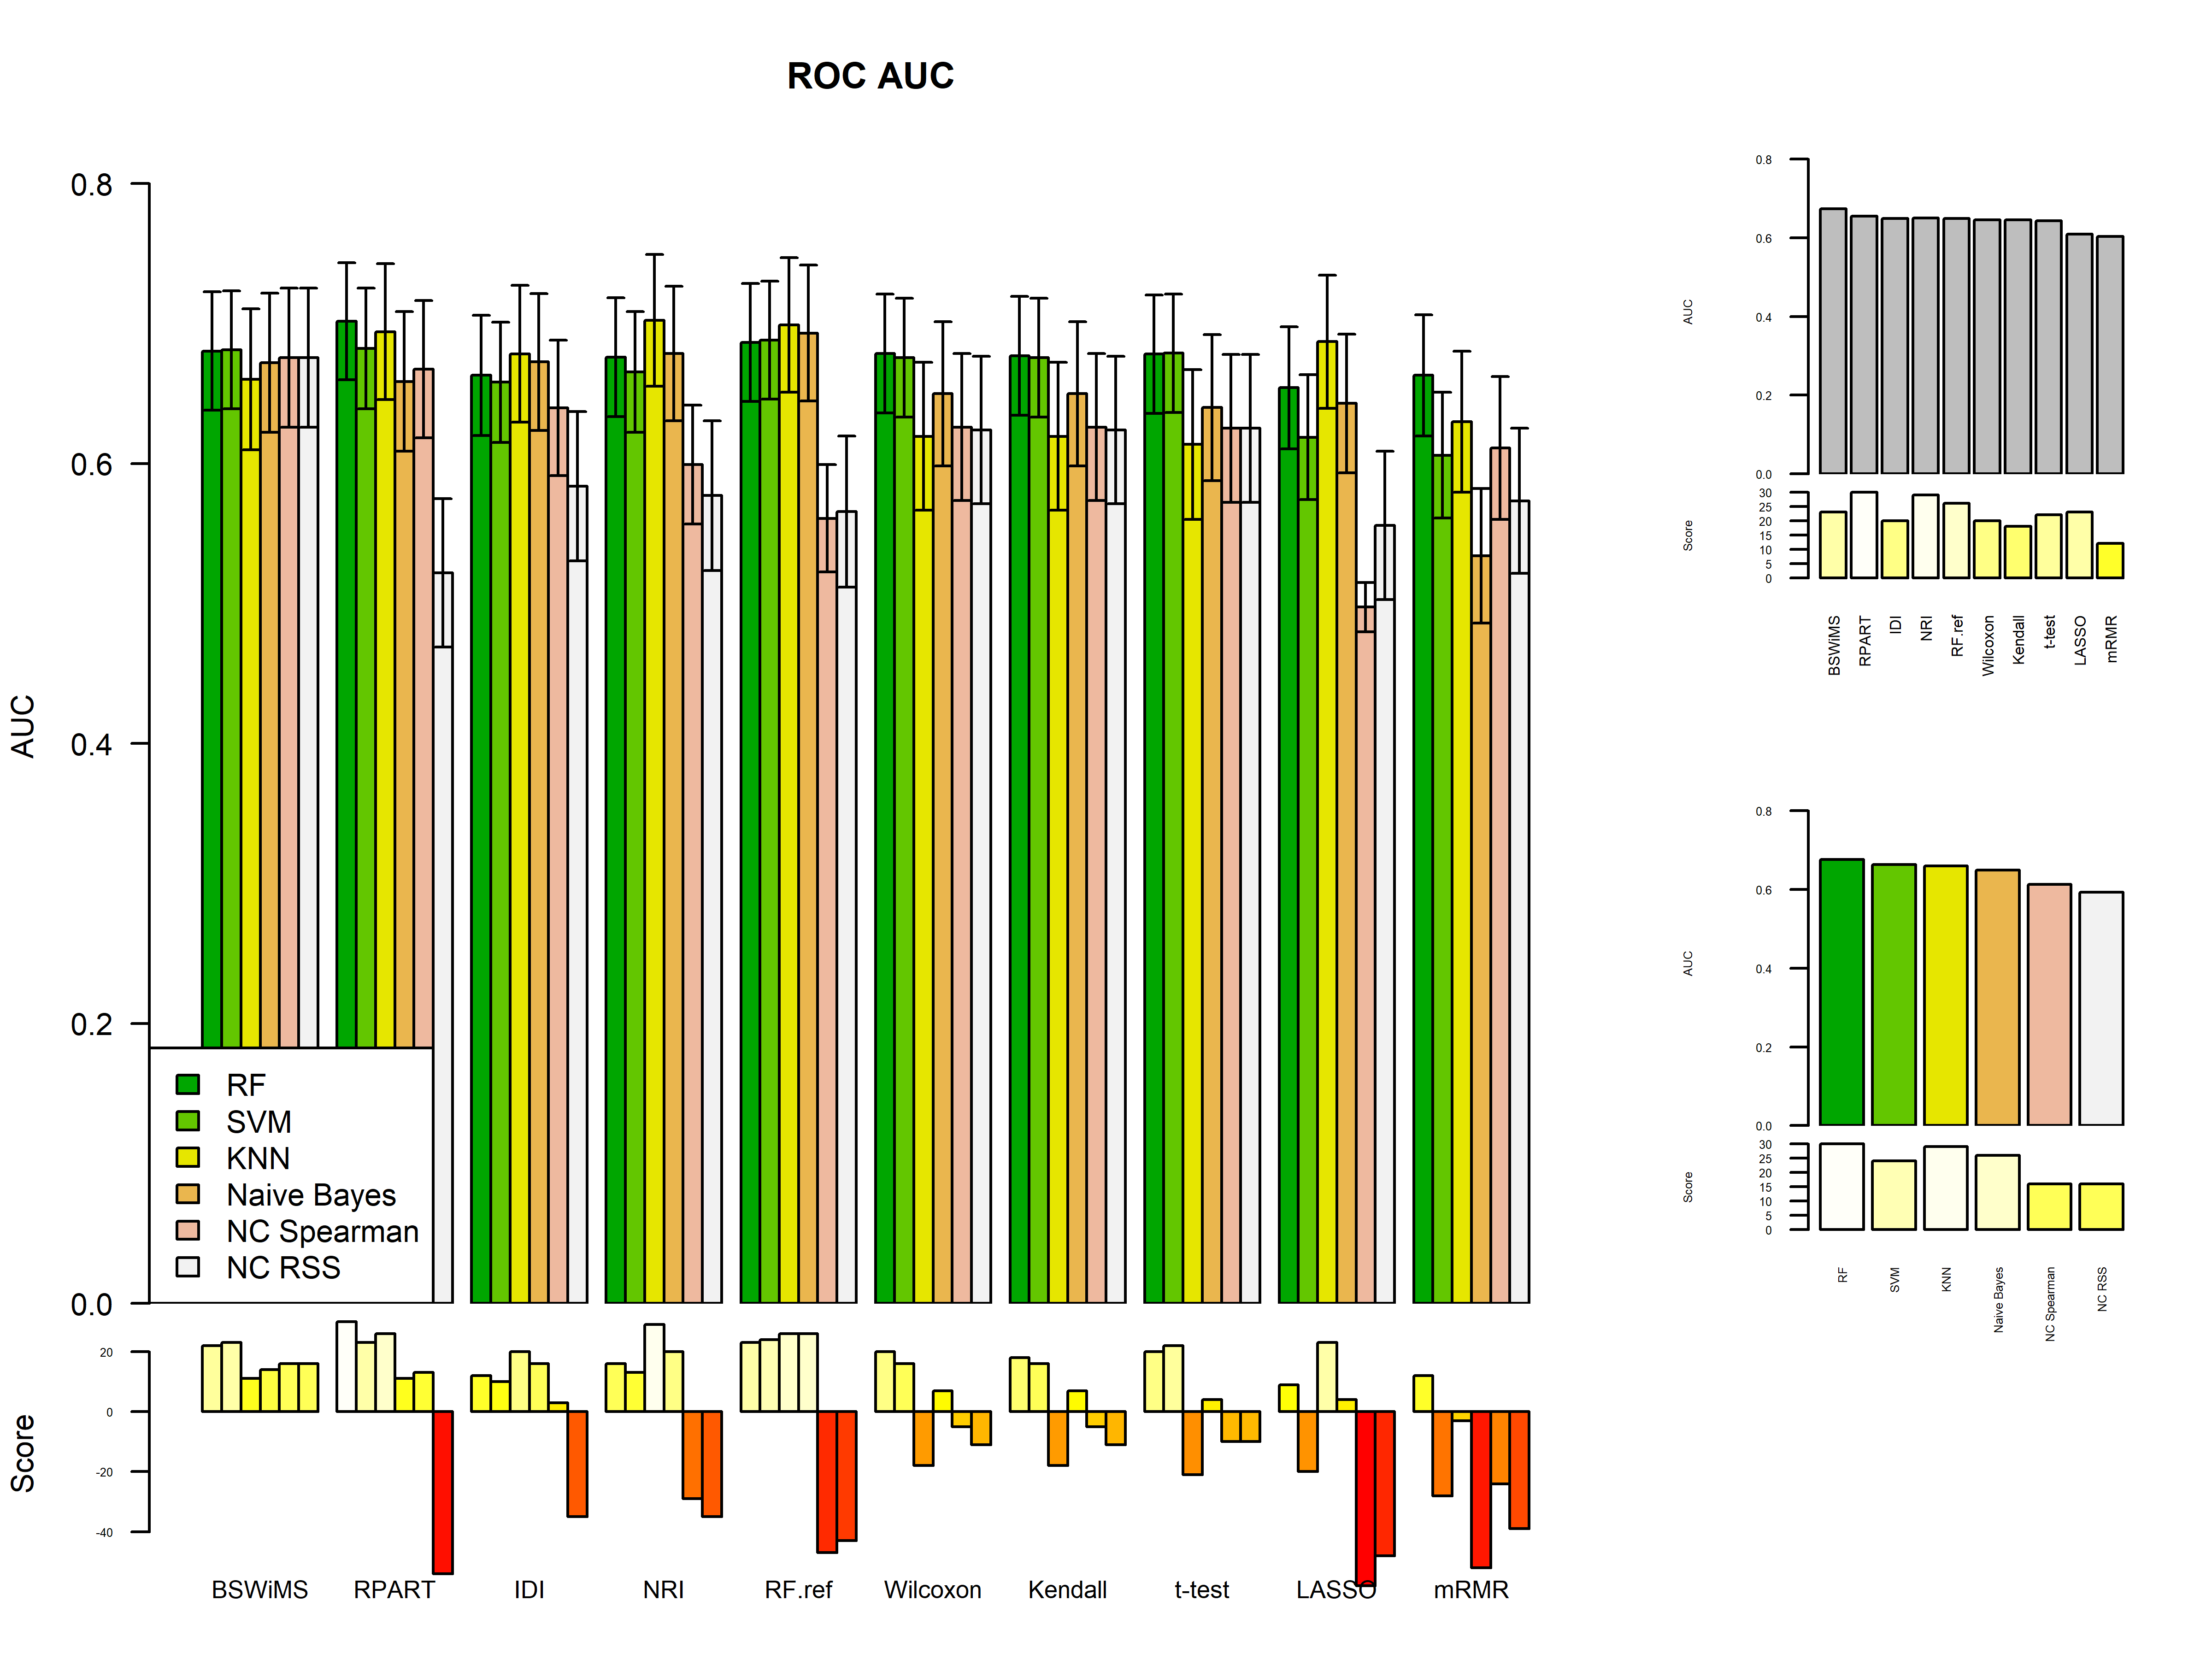
\includegraphics[width=5in,height=2in]{images/results/fresaConc.png}}
\centerline{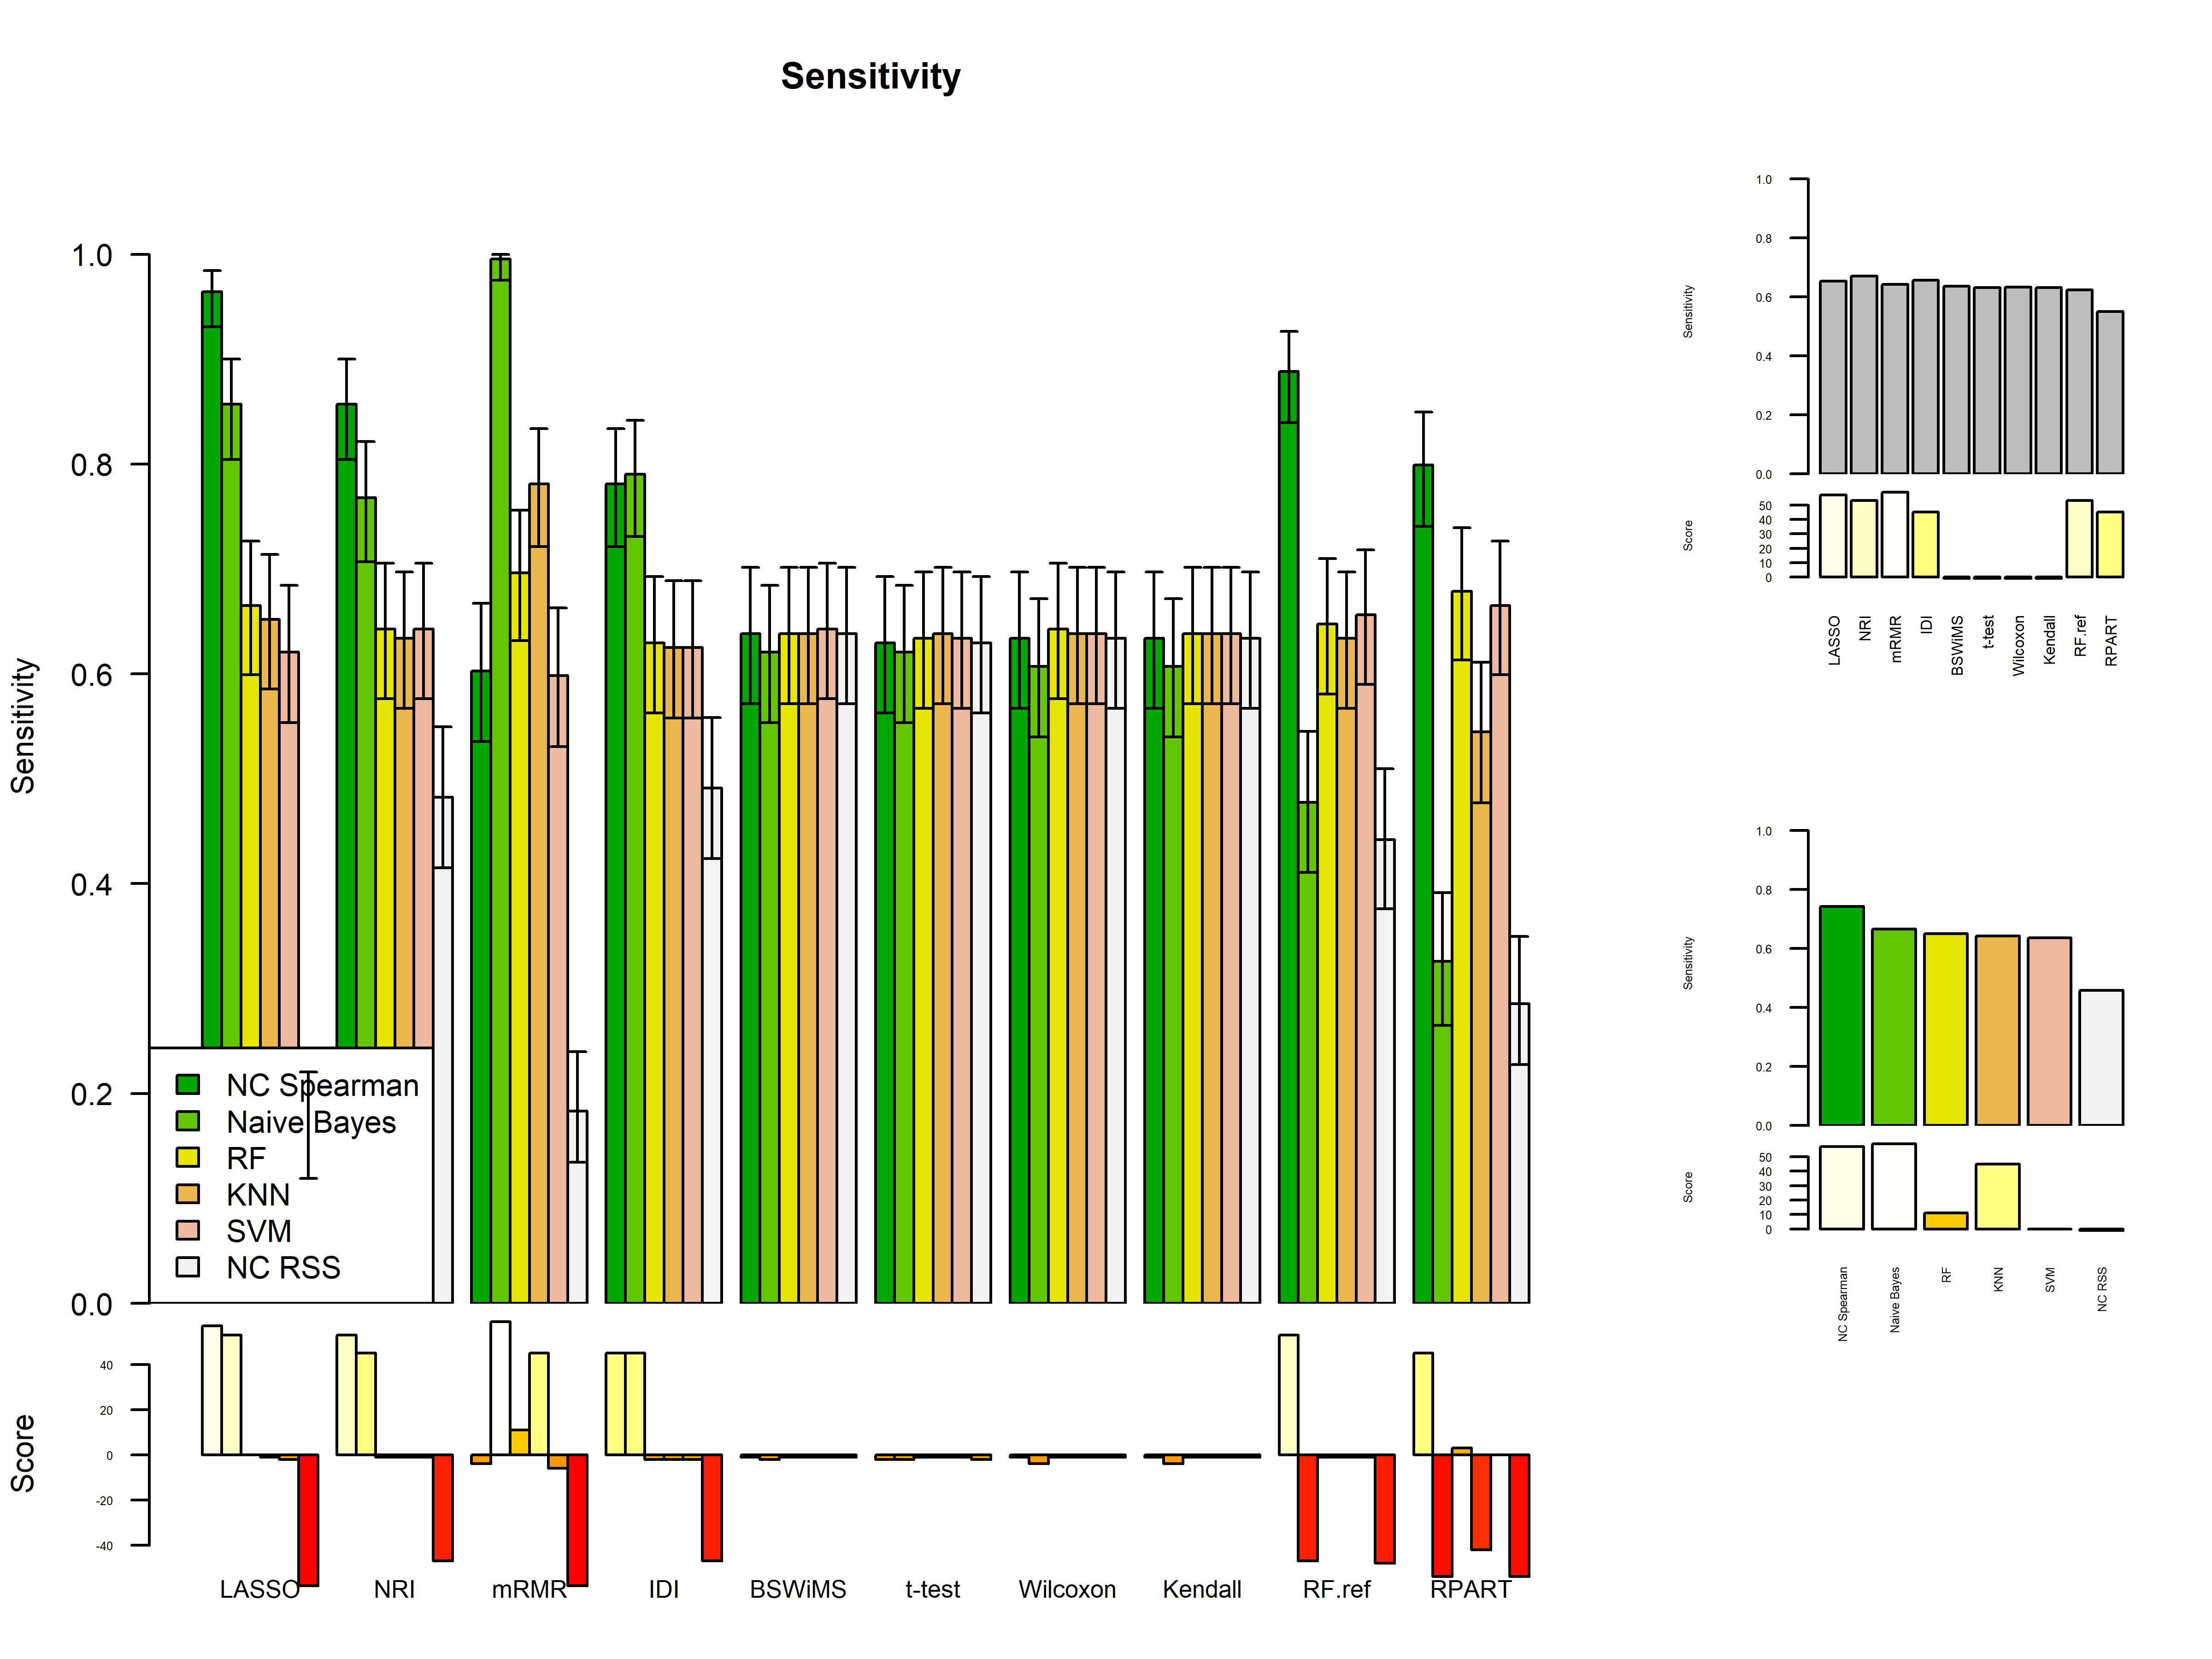
\includegraphics[width=5in,height=2in]{images/results/fresaSens.png}}
\centerline{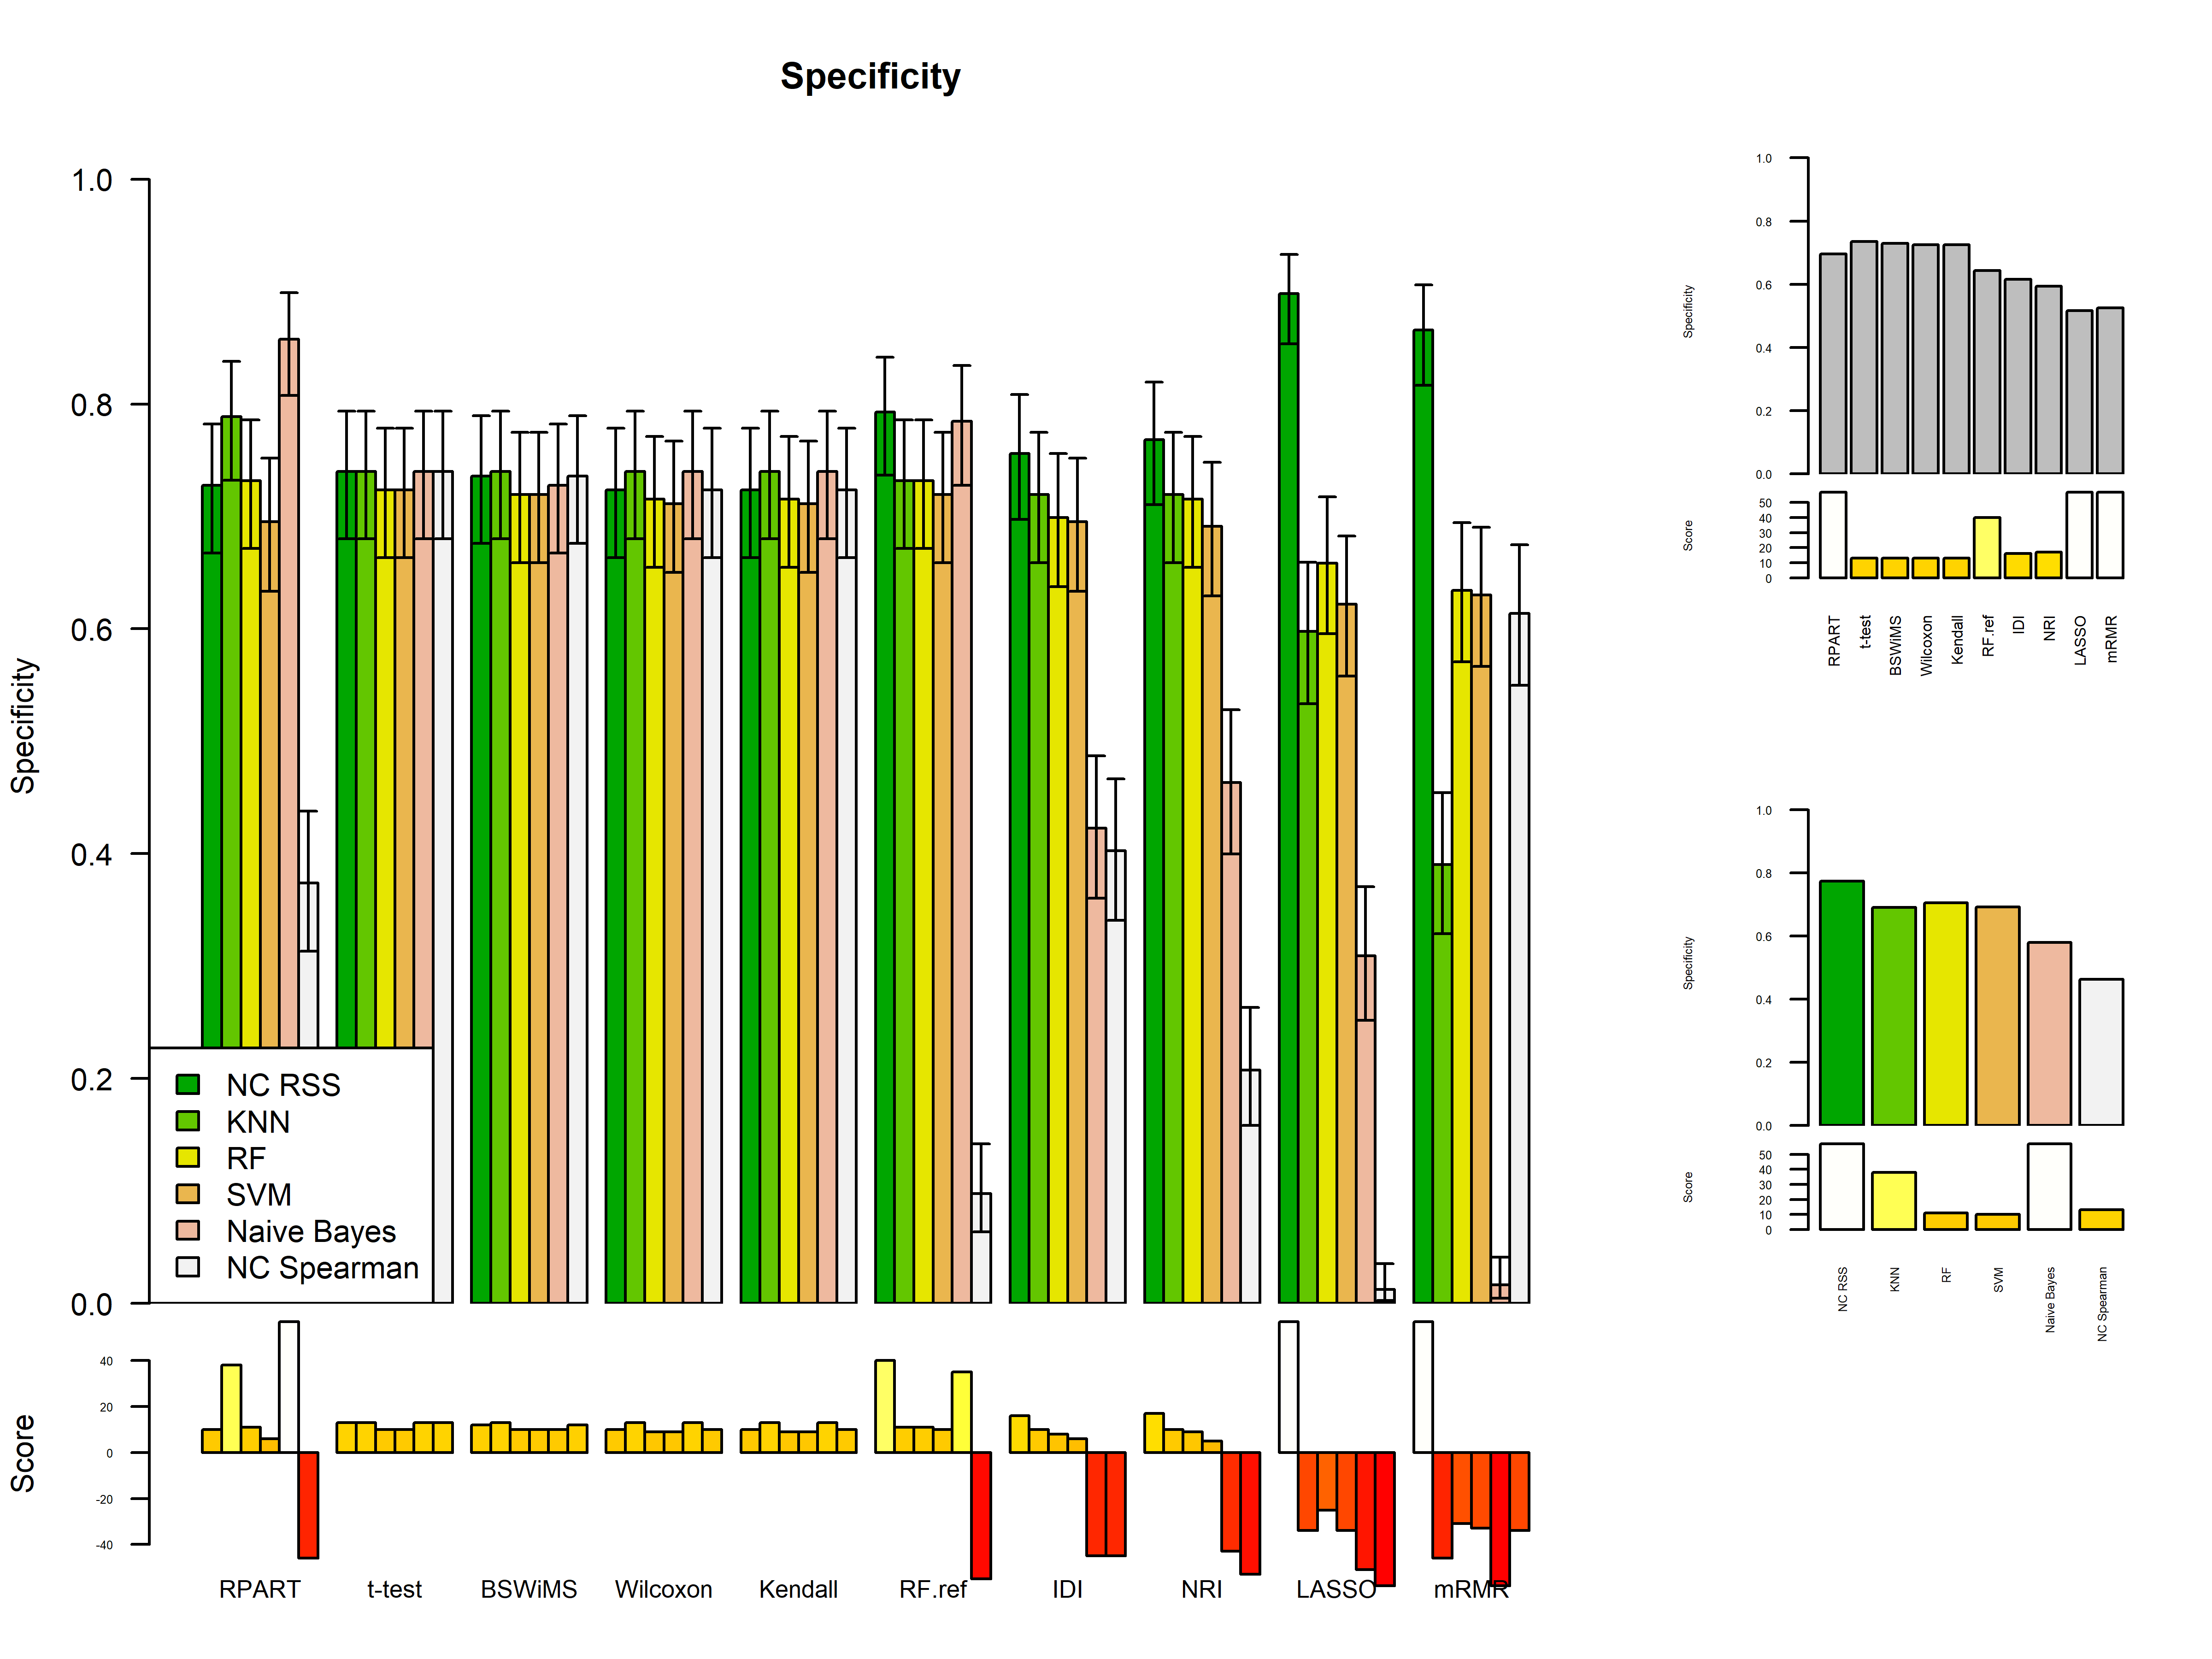
\includegraphics[width=5in,height=2in]{images/results/fresaSpec.png}}
\caption{{\bf ROC AUC, Sensitivity and Specificity of the FRESA.CAD Filter combinations} 
Comparison the ROC AUC, Sensitivity and Specificity Score obtained using the different combinations of classification methods plus filters of the FRESA.CAD Benchmarking with the complete ADNI dataset for the Cross-validation and using the top 2,500 SNPs as input}
\label{fig18}
\end{figure}
\newpage
A balanced comparison across metrics for the different classifiers can be seen in Figure 4.17. For the prediction models they all roughly perform the same with just the SVM varying from the others, but on the Filter method it can be seen how mRMR, Lasso, and RF filter give a worse Balanced Error than the others. BSWiMS features appear to be the best all around filter method.

\begin{figure}[!ht]
\centerline{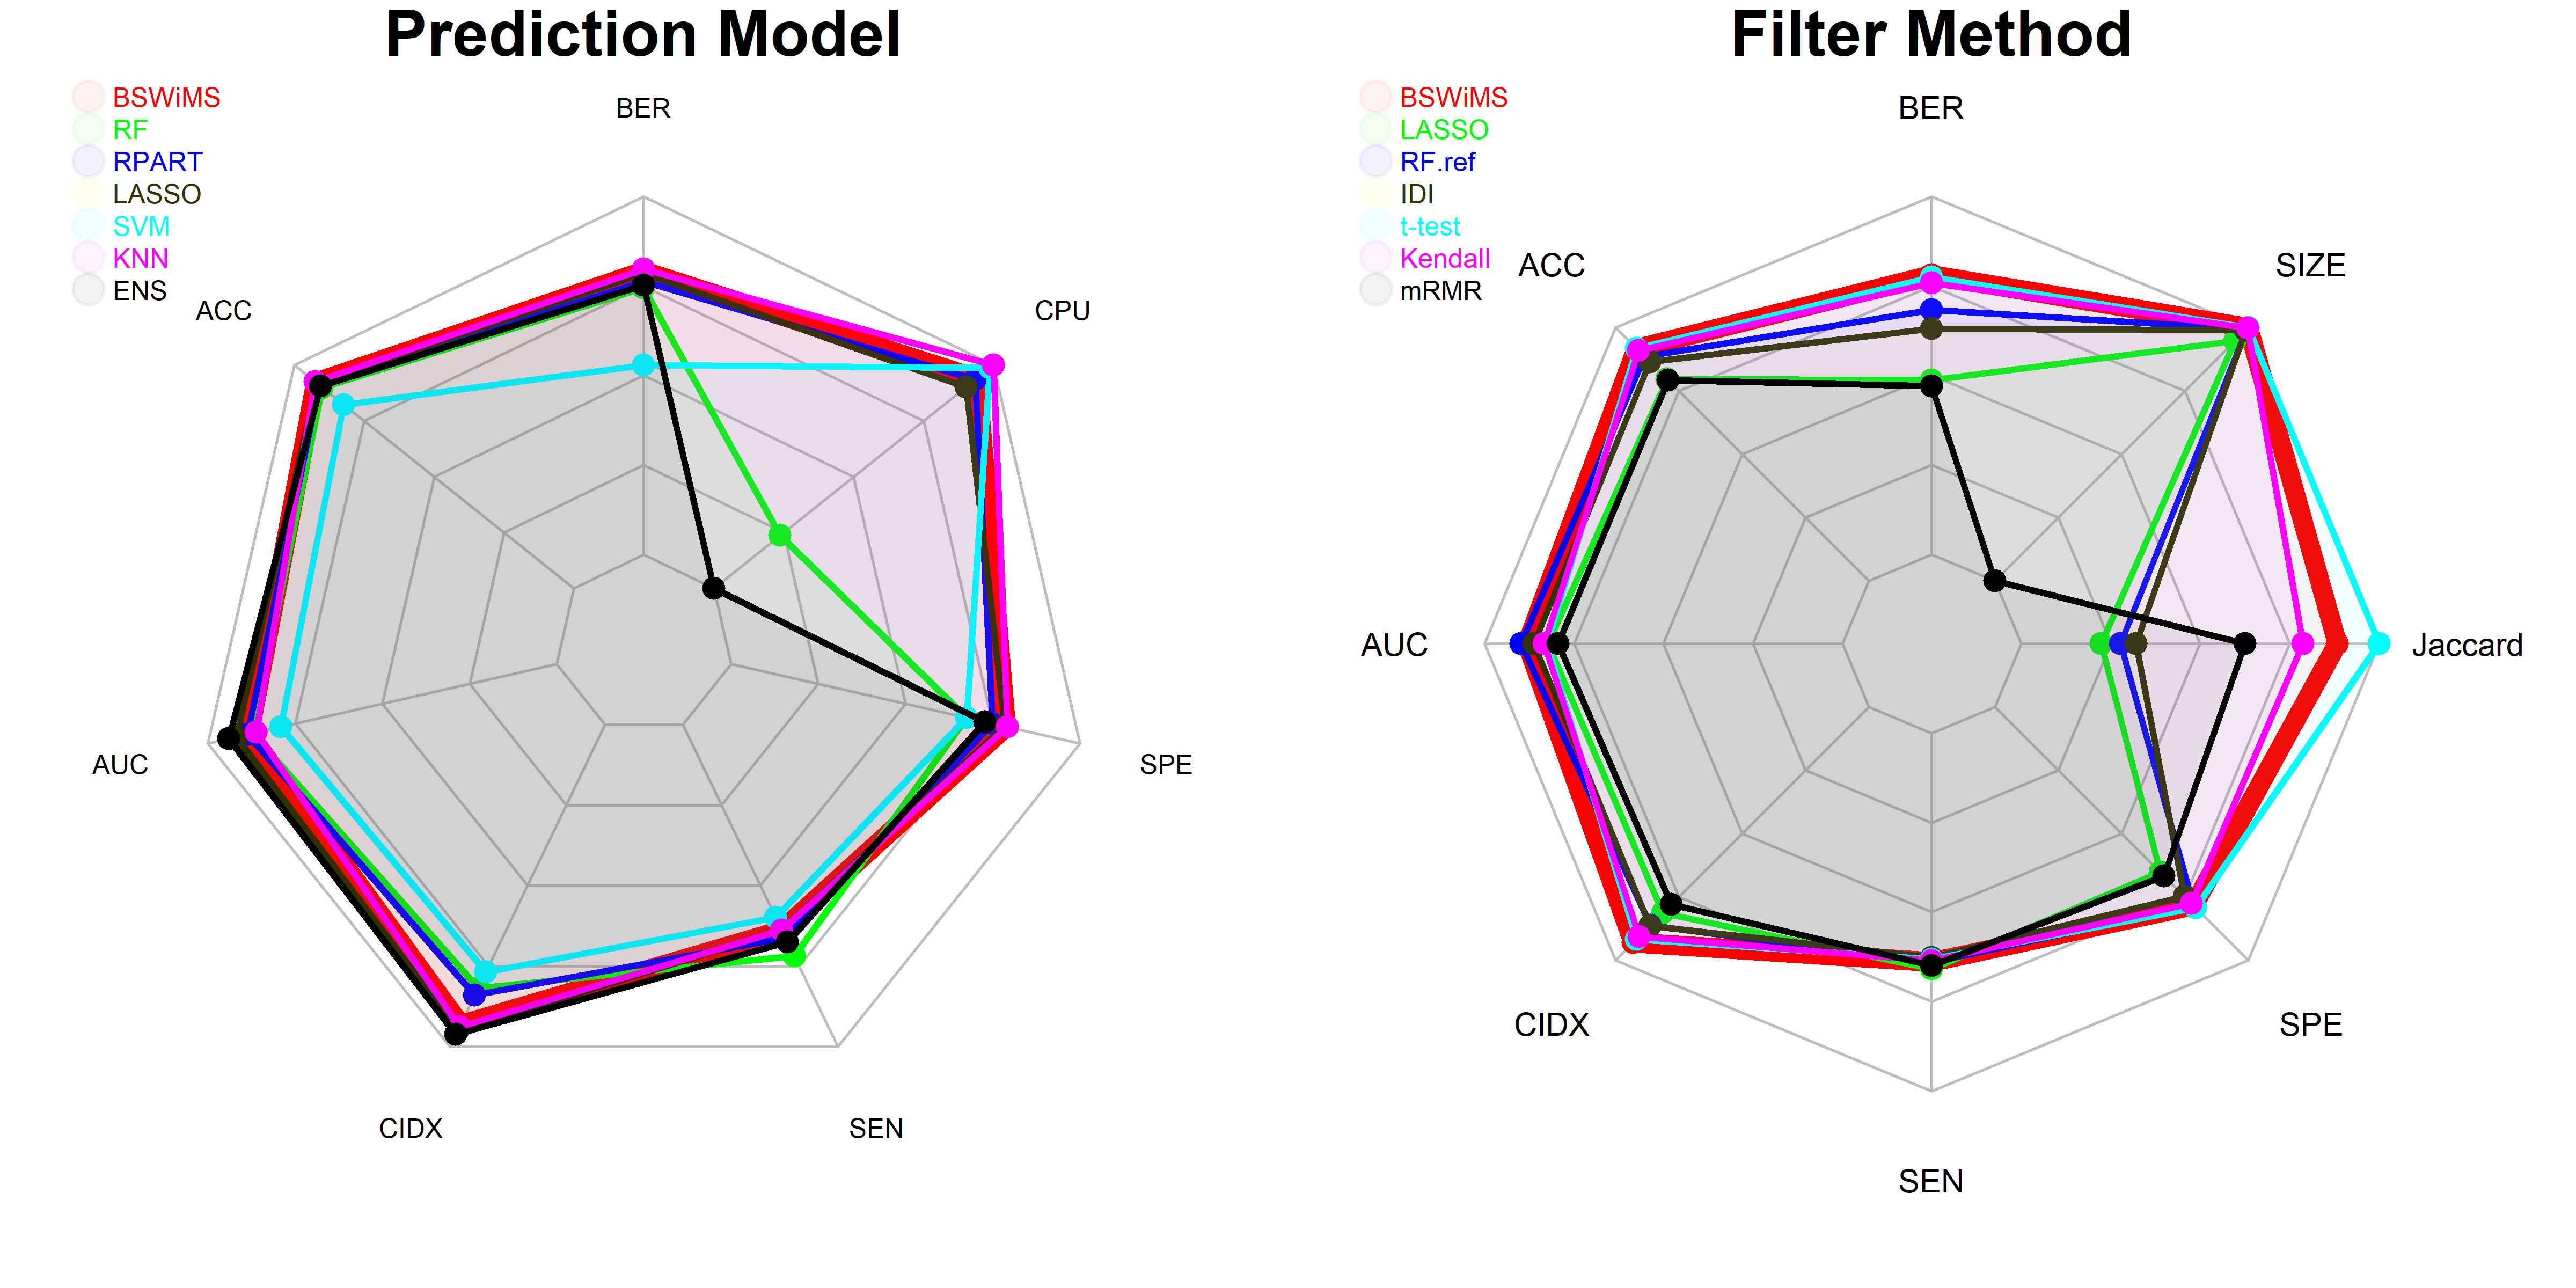
\includegraphics[width=4in]{images/results/fresaRadar.png}}
\caption{{\bf Comparison between the different classifiers and filters of the FRESA.CAD Benchmark } 
Radar plot analysing different metrics to evaluate the performance using different metrics as well as the CPU time between the different classifiers as well as filters of the FRESA.CAD Benchmarking with the complete ADNI dataset for the Cross-validation and using the top 2,500 SNPs as input}
\label{fig19}
\end{figure}

The main goal of the analysis is not only to classify the samples into the two types of diagnosis to better analyze it and treat it, but most importantly to detect precisely which are the given gene variants that could be responsible for the disease as well as to ensure the chosen SNPs have a biological and chemical basis. As such further analysis on the Feature selection process gives insight into those SNPs selected by the different methods as being critical to the decision-making boundary, which enables doctors to precisely genotype only those given genes when a patient comes in and get the results quickly, and also allows researchers to delve into the biochemical reasons of new candidates if found.

The result of one such analysis is shown in Figure 4.18, and shows that there are multiple variants being used by the different methods and they have statistical significance. Definitely the APOE $\epsilon4$(rs429358) marker is being chosen by all the classification methods and this comes as no surprise due to its strong impact on the prediction. RPART is using multiple genes which are not being selected by other methods, and LASSO is using more SNPs but which are also being selected by the other methods. Both of these approaches are giving good results in the classification. mRMR is selecting all of the most frequent markers, but as seen before this does not mean it will perform better. Interesting candidates for further analysis could be rs67636621, rs76566842 and rs16905109 based on this figure.

\begin{figure}[!ht]
\centerline{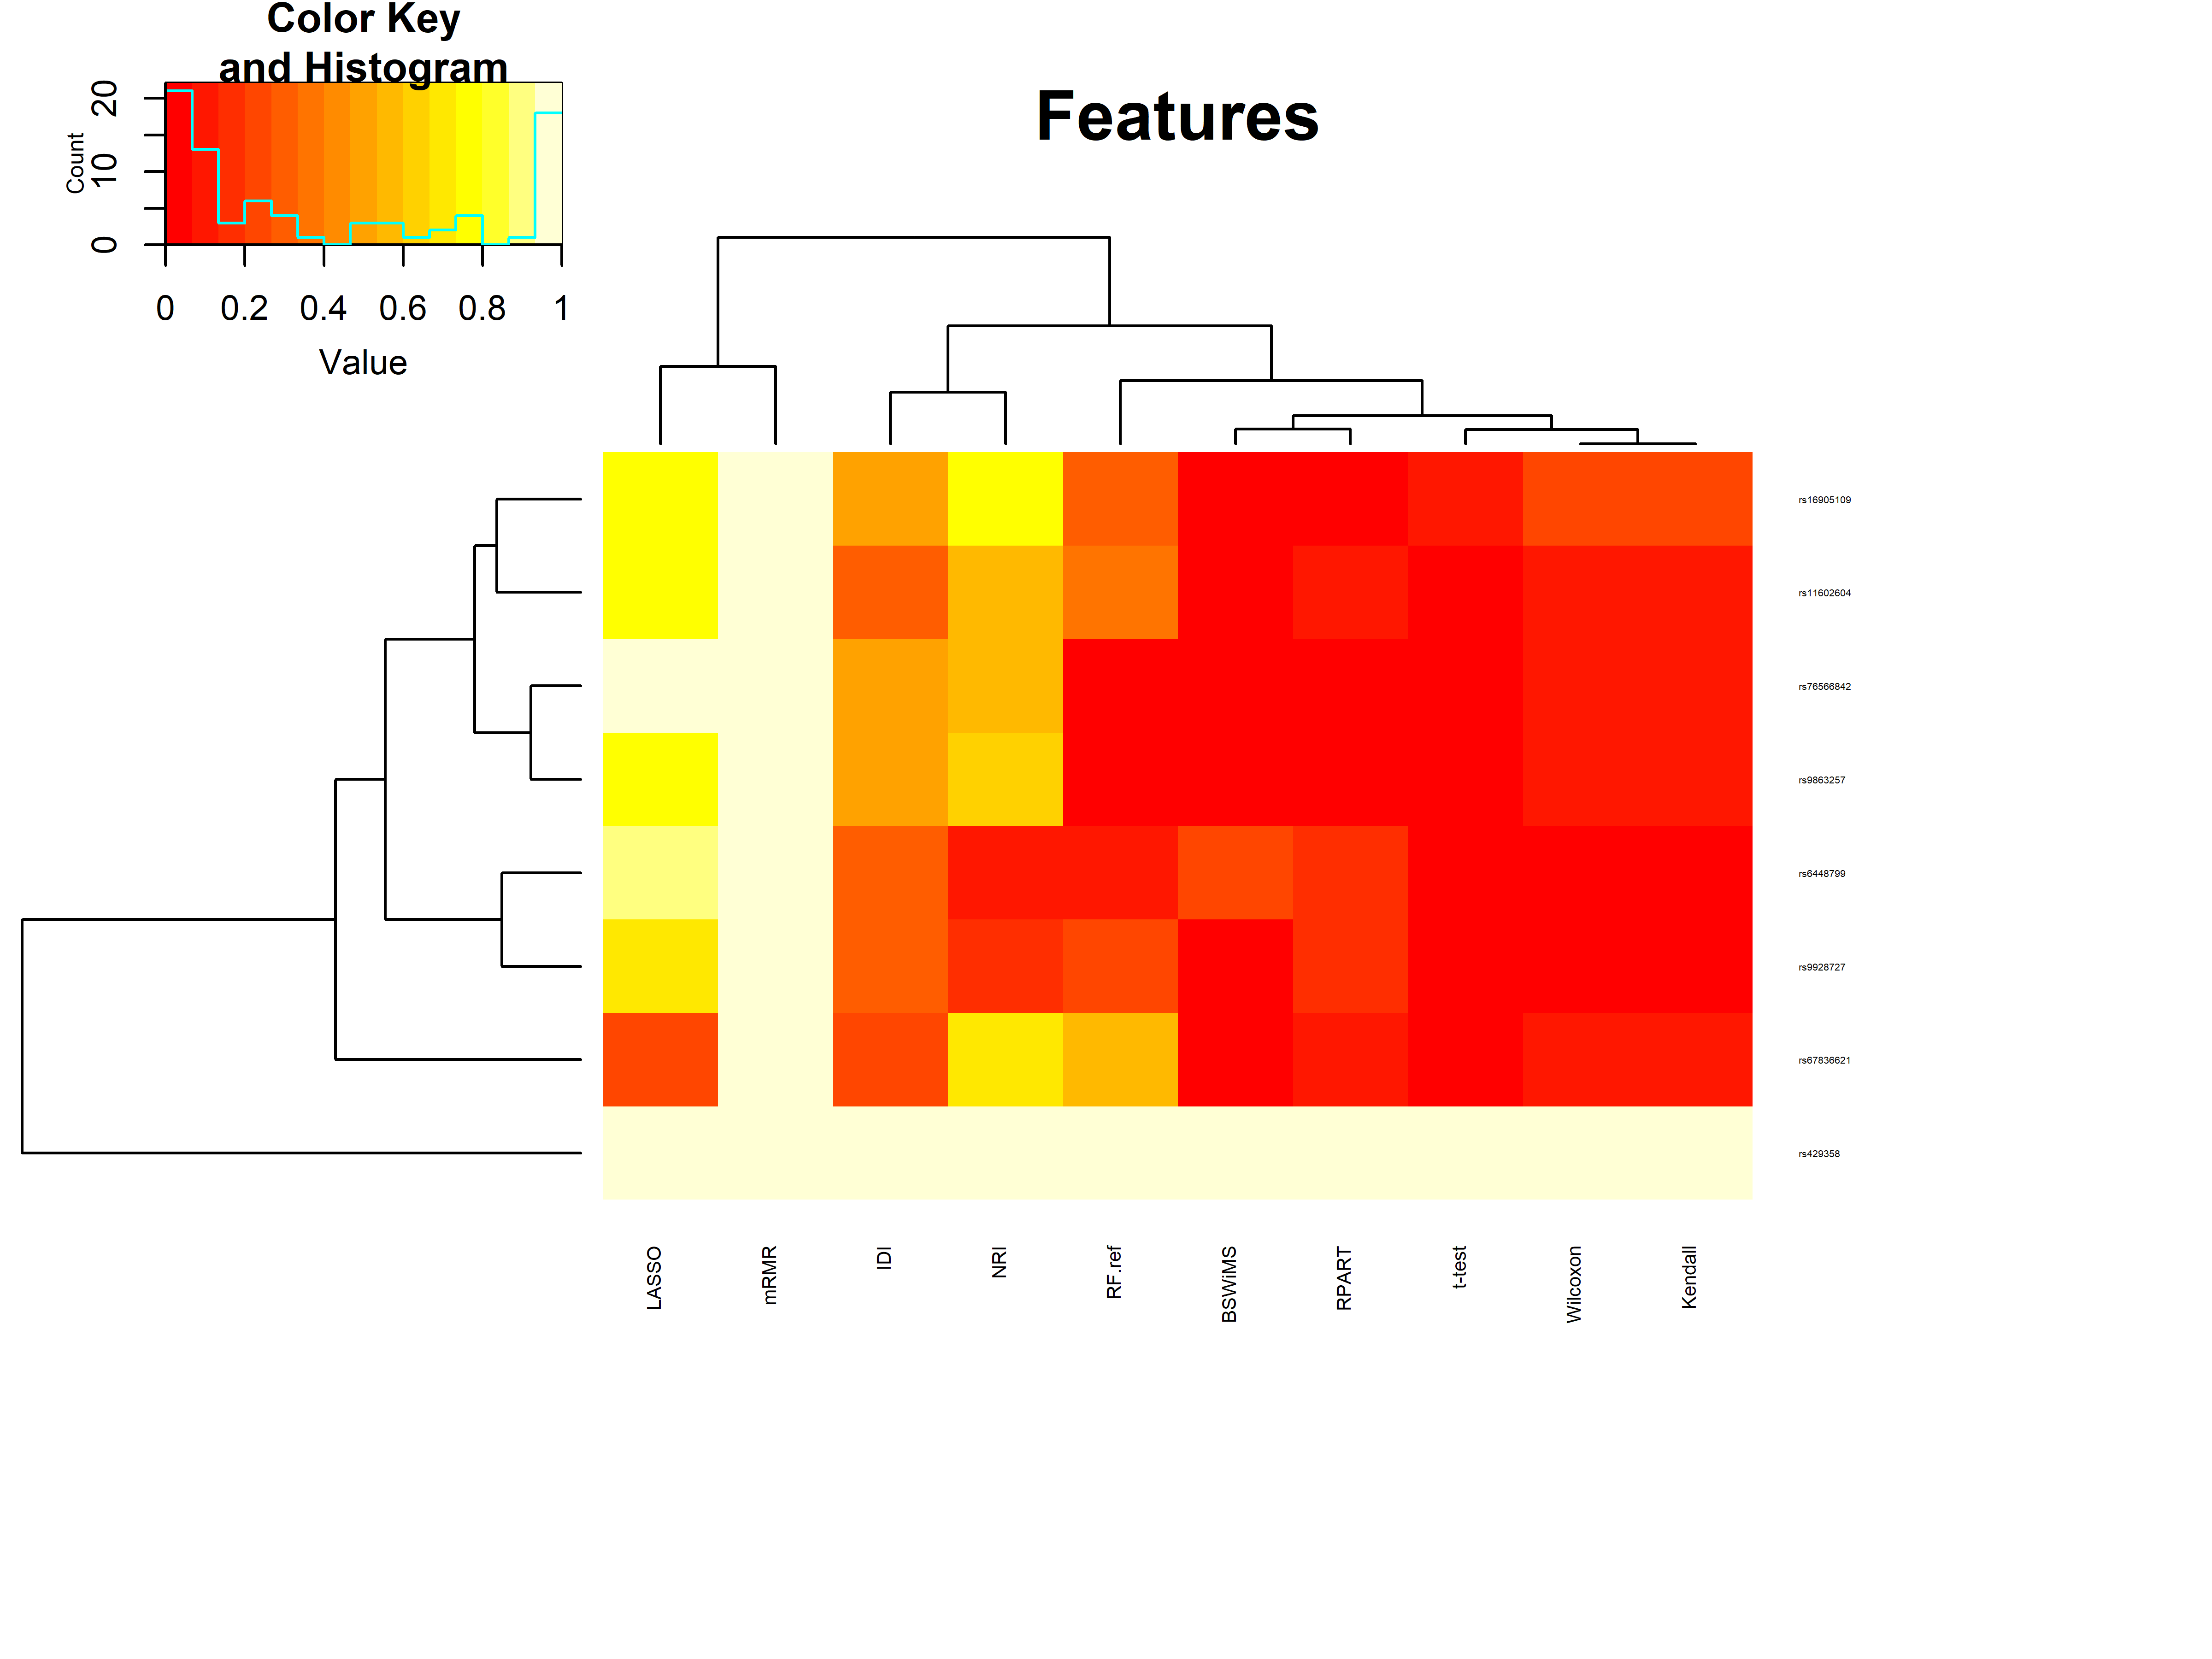
\includegraphics[width=4in]{images/results/fresaSNPs.png}}
\caption{{\bf SNPs chosen more than 10\% of the time as features of the FRESA.CAD Benchmark} 
Heatmap of the main SNPs being chosen across all the classifiers. The Y axis are the main SNPs being selected while the X axis represents the different classifiers of the FRESA.CAD Benchmarking with the complete ADNI dataset for the Cross-validation and using the top 2,500 SNPs as input}
\label{fig20}
\end{figure}
 
 
To further analyze the top candidates Table 1 contains the results of the 8 most important SNPs that are found (The only ones selected by more than 10\% of the models. Most of them have a quite high significance according to the Wilcoxon test when doing Univariate Analysis. The APOE $\epsilon4$ gene definitely gives a very strong predictive power, and the remaining genes are then used to further improve the model. One note: The ROC AUC value per SNP is not directly comparable to previous ROC AUC values shown before due to the calculation procedure, as it will be further shown in the next analysis. Also, while some have a better Wilcoxon result that does not necessarily relate to a higher classification power or vice-versa, as it happens with rs11602604. The results seem to prove the current knowledge that APOE $\epsilon4$ is the main factor with other SNPs complementing with small effects, thus it makes sense that models always select it. And to complement it as the other results also show how the models with more SNPs slightly outperform the smaller models

\begin{table}[ht!]
    \begin{center}
        \begin{tabular}{|c|c|c|c|}
        \hline
        \textbf{SNP}   &  \textbf{ROC AUC} &  \textbf{WILCOX} &  \textbf{FREQ} \\ \hline
rs429358   &	0.6961 &	0       &	1.000 \\ \hline
rs67836621  &	0.5815 &	8e-04   &	0.298 \\ \hline
rs9928727	&	0.5787 &	9e-04   &	0.269 \\ \hline
rs11602604	&	0.5783 &	3e-04   &	0.321 \\ \hline
rs6448799	&	0.5751 &	6e-04   &	0.288 \\ \hline
rs16905109	&	0.5484 &	0.0011  &	0.383 \\ \hline
rs76566842	&	0.534  &	0.1619  &	0.327 \\ \hline
rs9863257	&	0.5321 &	0.1955  &	0.323 \\ \hline
        \end{tabular}
    \end{center}
  \caption{Top SNPs selected as important features for the full ADNI Dataset}
  \label{topsnps}
\end{table}

\newpage
The second analysis to perform is on the reduced validation dataset without samples from the IGAP using the top 1,000 SNPs. As before, this has the problem of being a small sample size. Contrasting the previous results are the ROC Curves from this dataset as shown in Figure 4.19 and Figure 4.20. The results are much lower, in the order of 0.50\~0.60. In this case only BSWiMS, RPART and the Ensemble give useful predictions. This shows again the complexity of the given problem with a small, unbalanced dataset for validation due to independent from the statistical analysis and reinforces the results from previous analysis.

 \begin{figure}[!ht]
\centerline{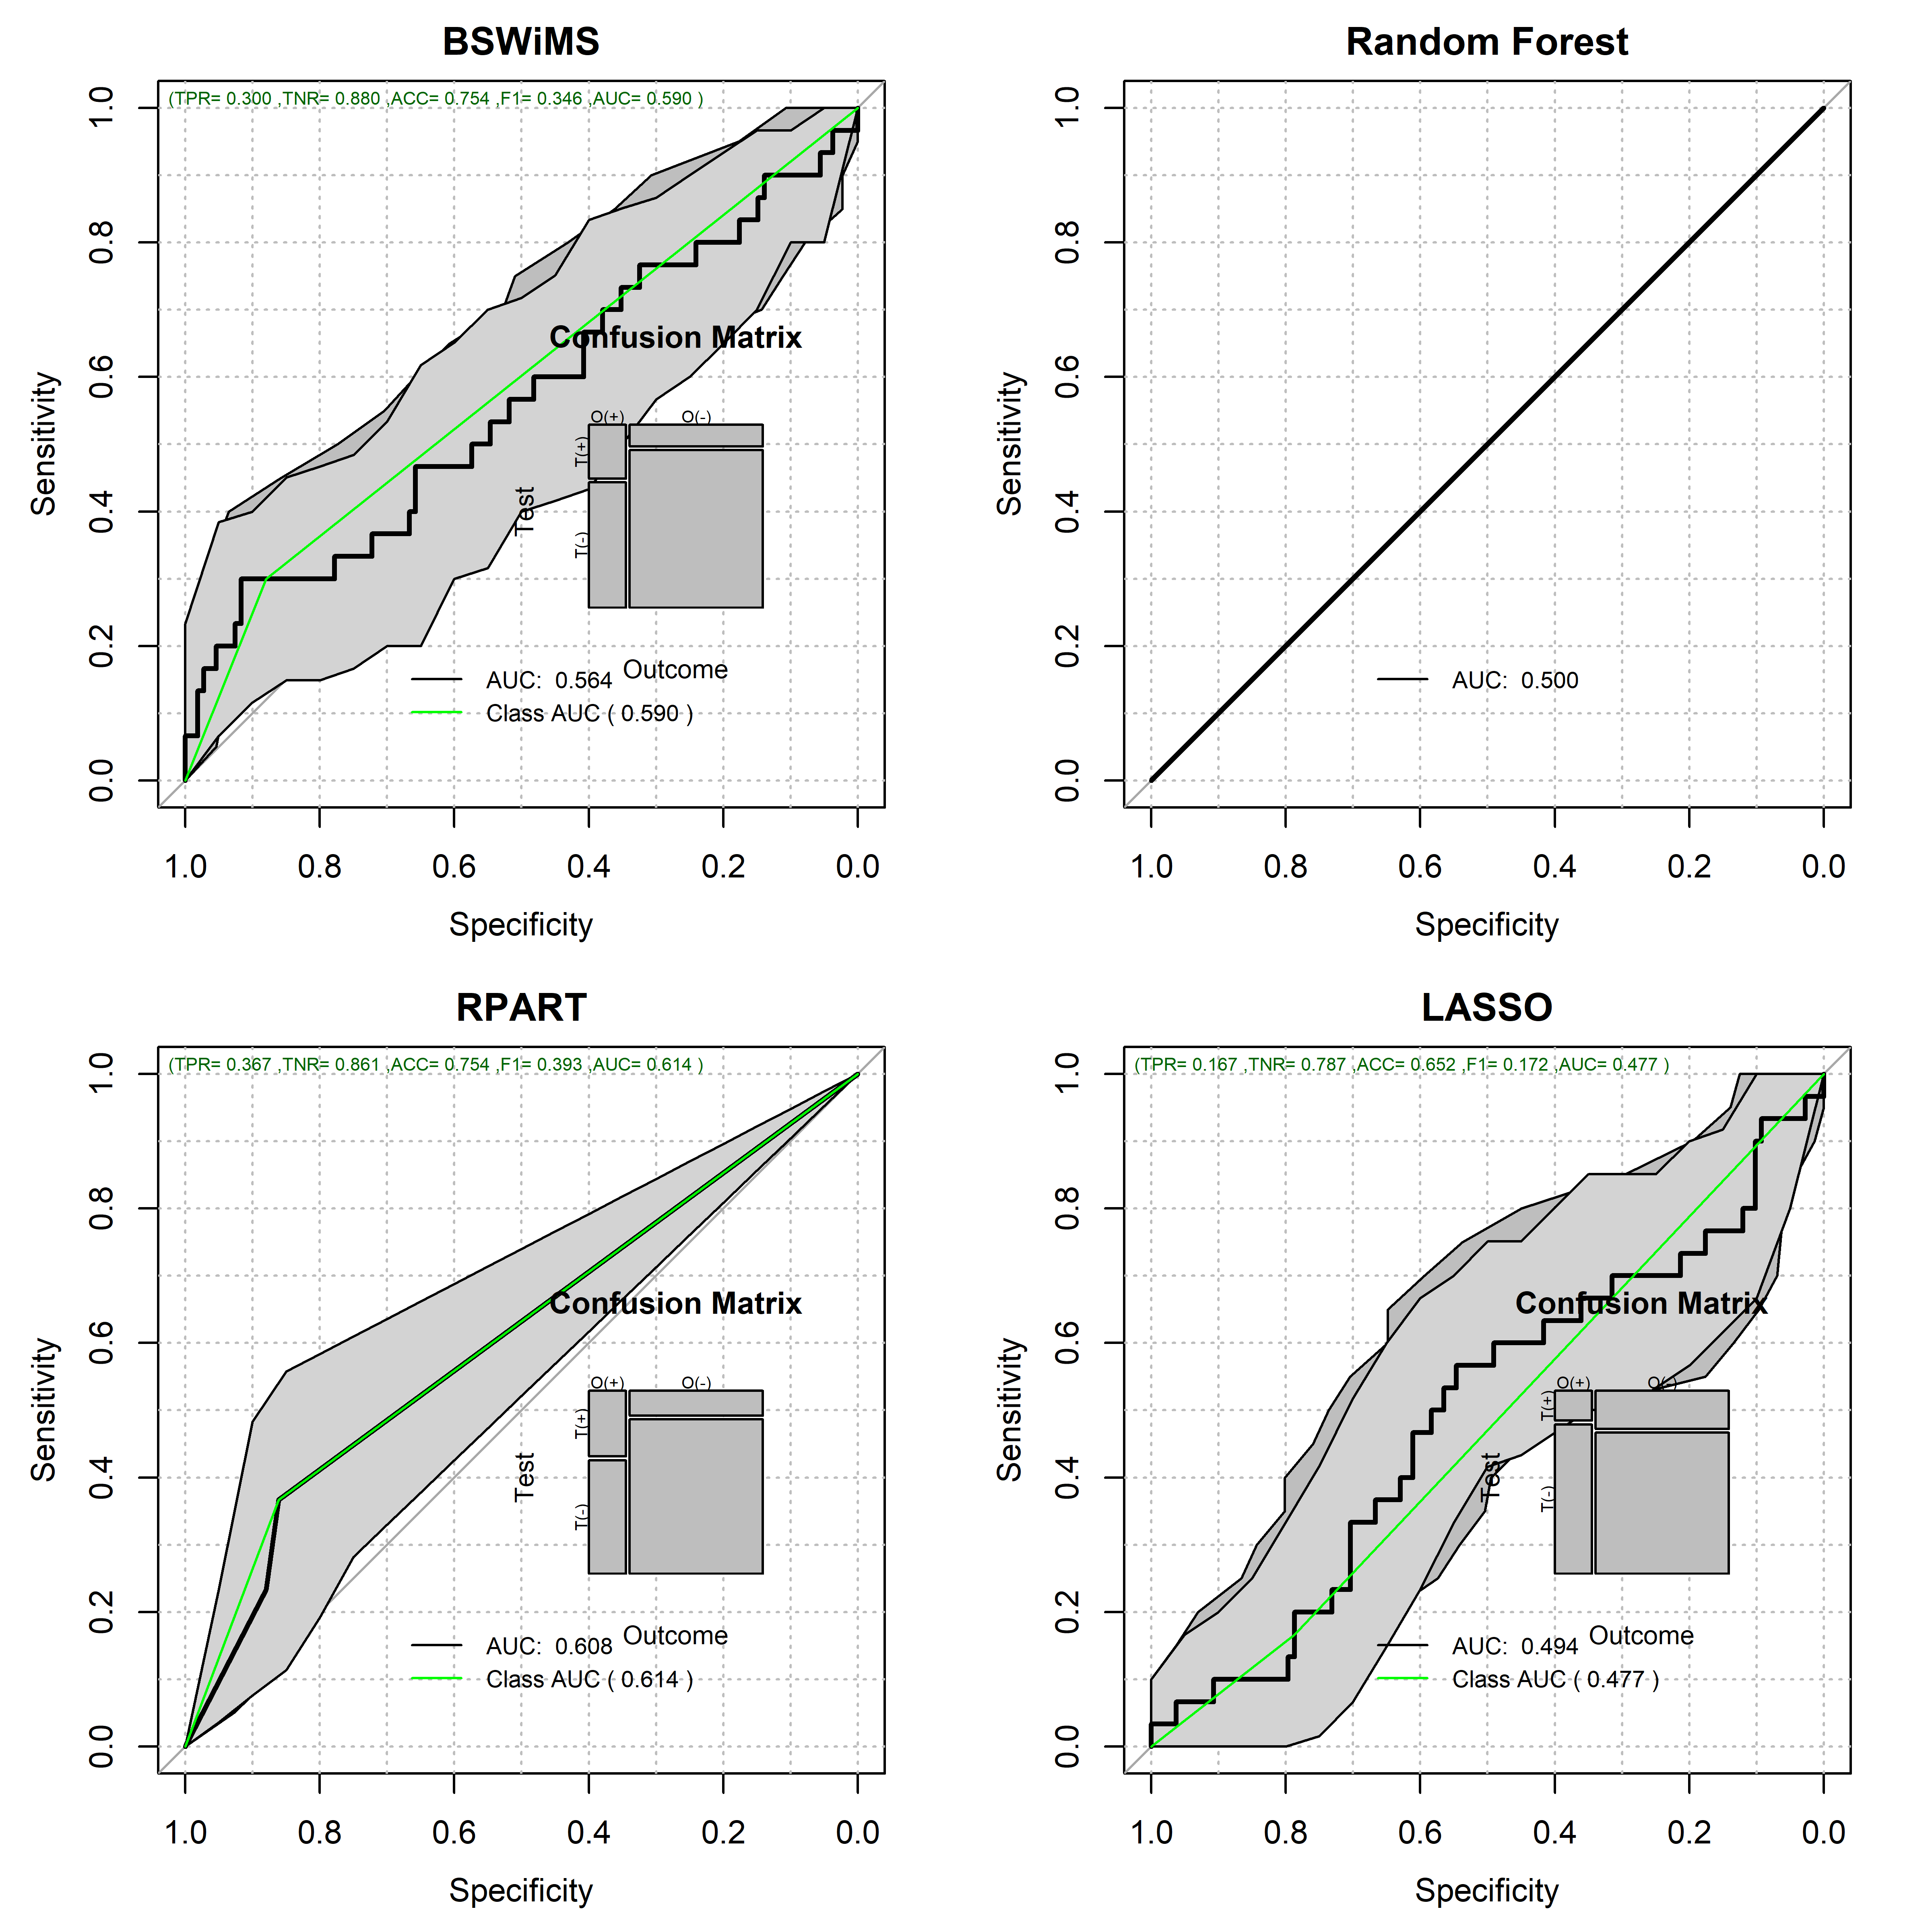
\includegraphics[width=3in]{images/results/fresaCurves1Val.png}}
\caption{{\bf Validation ROC Curves for the FRESA.CAD Benchmarking Classifiers} 
ROC Curves obtained using BSWiMS, Random Forest, RPART and LASSO of the FRESA.CAD Benchmarking with the validation dataset for the Cross-validation and using the top 1,000 SNPs as input}
\label{fig24}
\end{figure}

 \begin{figure}[!ht]
\centerline{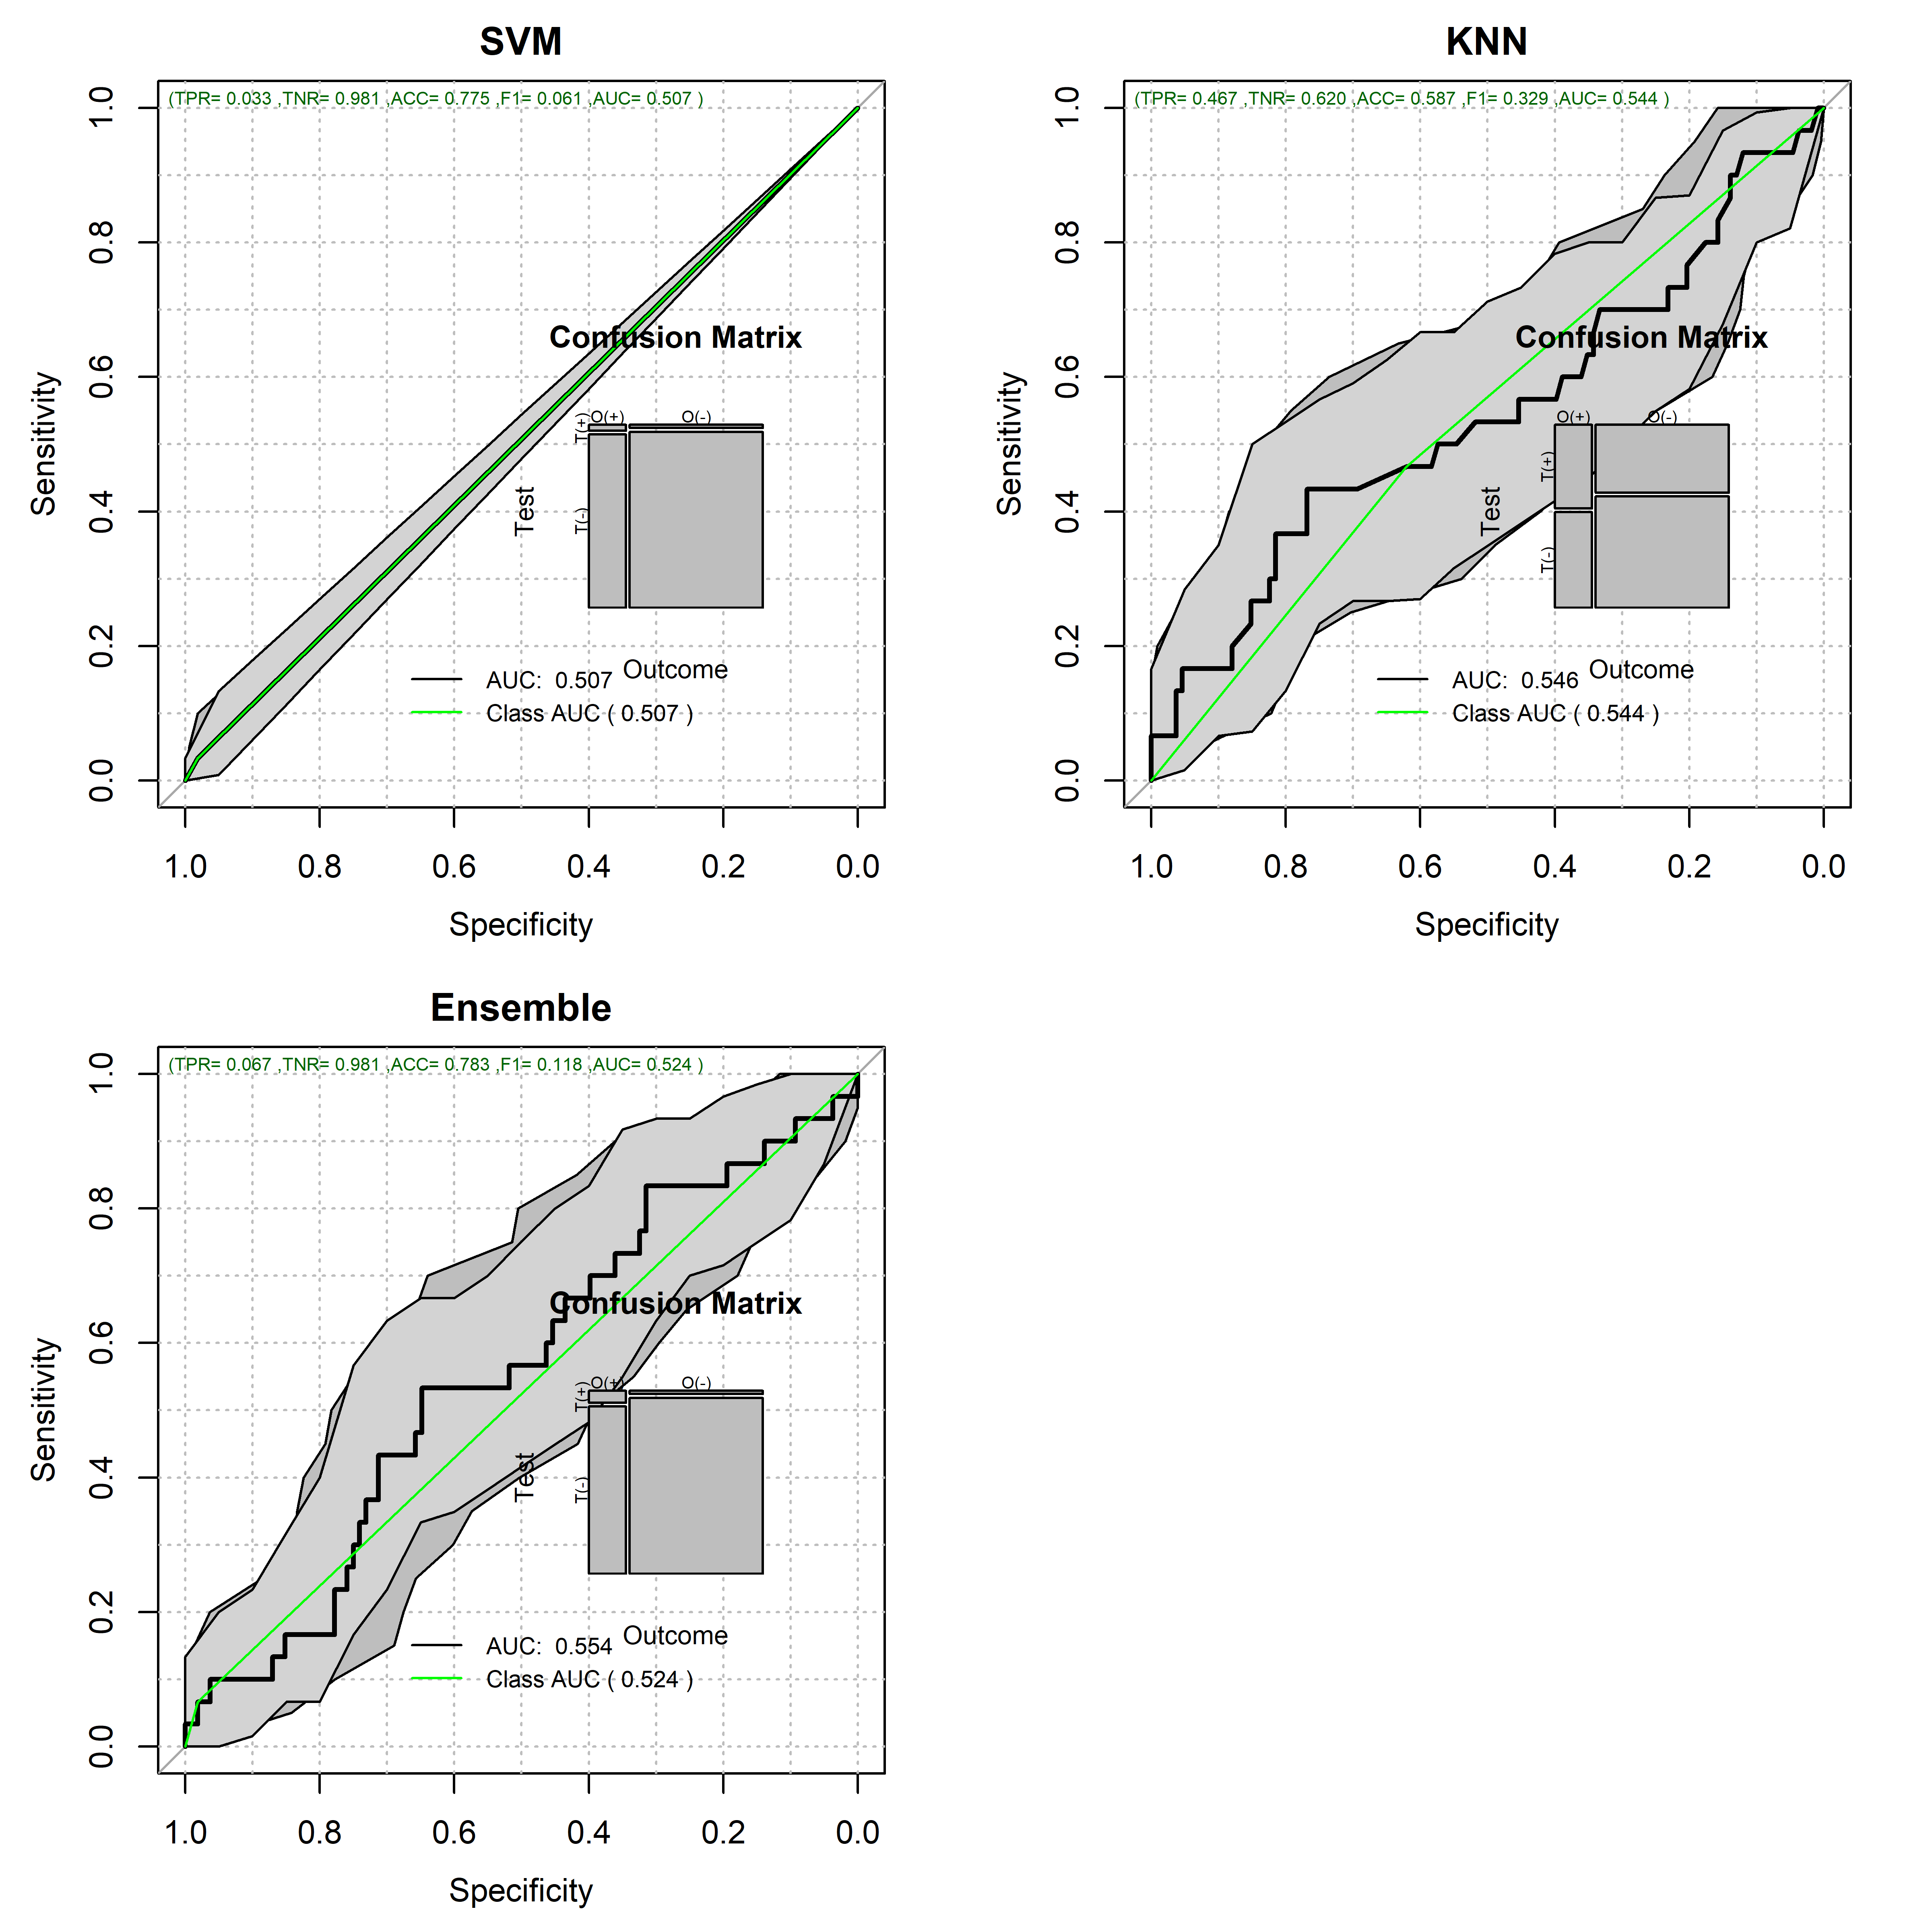
\includegraphics[width=3in]{images/results/fresaCurves2Val.png}}
\caption{{\bf Validation ROC Curves for the FRESA.CAD Benchmarking Classifiers (Continued)} 
ROC Curves obtained using SVM, KNN and the Ensemble of the FRESA.CAD Benchmarking with the validation dataset for the Cross-validation and using the top 1,000 SNPs as inputs}
\label{fig25}
\end{figure}

Figure 4.21 and 4.22 reinforce this by showing the different metrics. As seen the accuracy tends to be quite high, but this is due to the class unbalance. Thus the Balanced error and the ROC give better metrics.  BSWiMS and RPART are shown to have the lowest Balanced Error and the best ROC AUC scores, followed by the Ensemble. Thus for this sub problem either model would be better than the Ensemble in contrast to the previous Analysis. An important detail to notice is the larger confidence intervals, as the dataset has a lower number of features this confidence interval is higher and as such it could be possible that all models perform quite equally when tested outside outside of this dataset. The same happens with the filter combinations, where it can be seen that there is no clear filter better than the rest with certainty, although Naive Bayes tends to show better results than the others.

 \begin{figure}[!ht]
\centerline{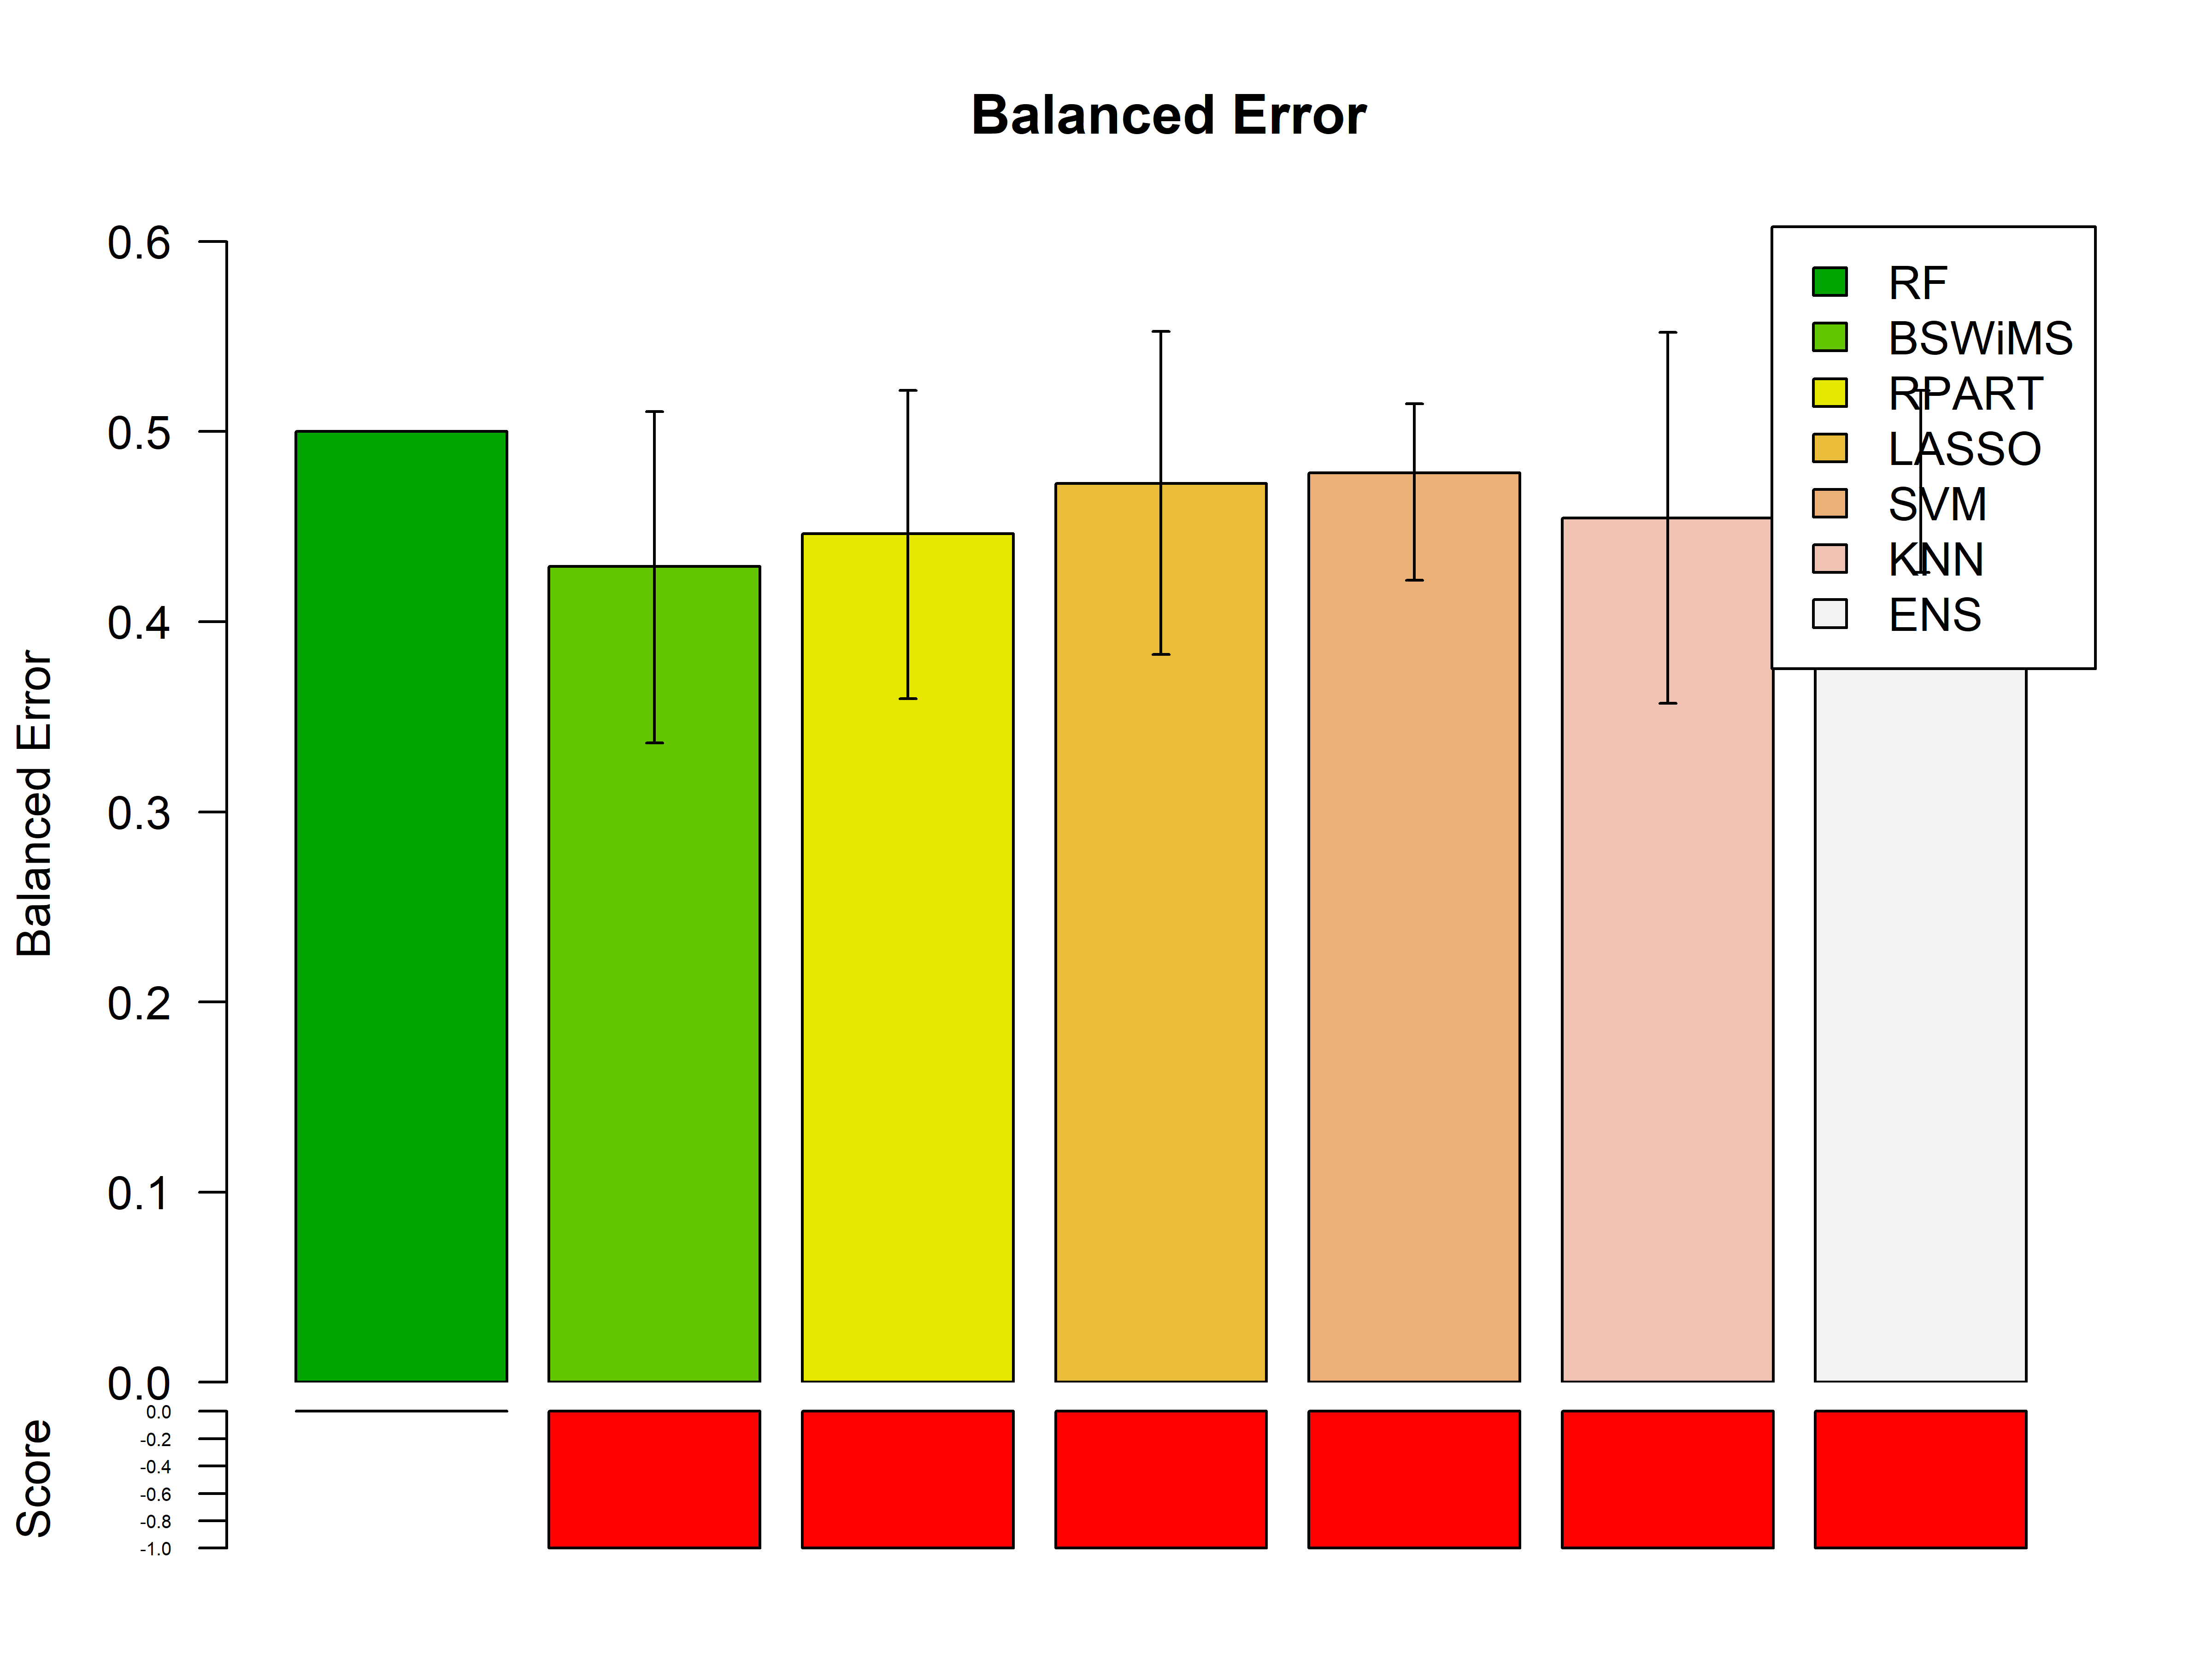
\includegraphics[width=5in,height=2in]{images/results/fresaBEVal.png}}
\centerline{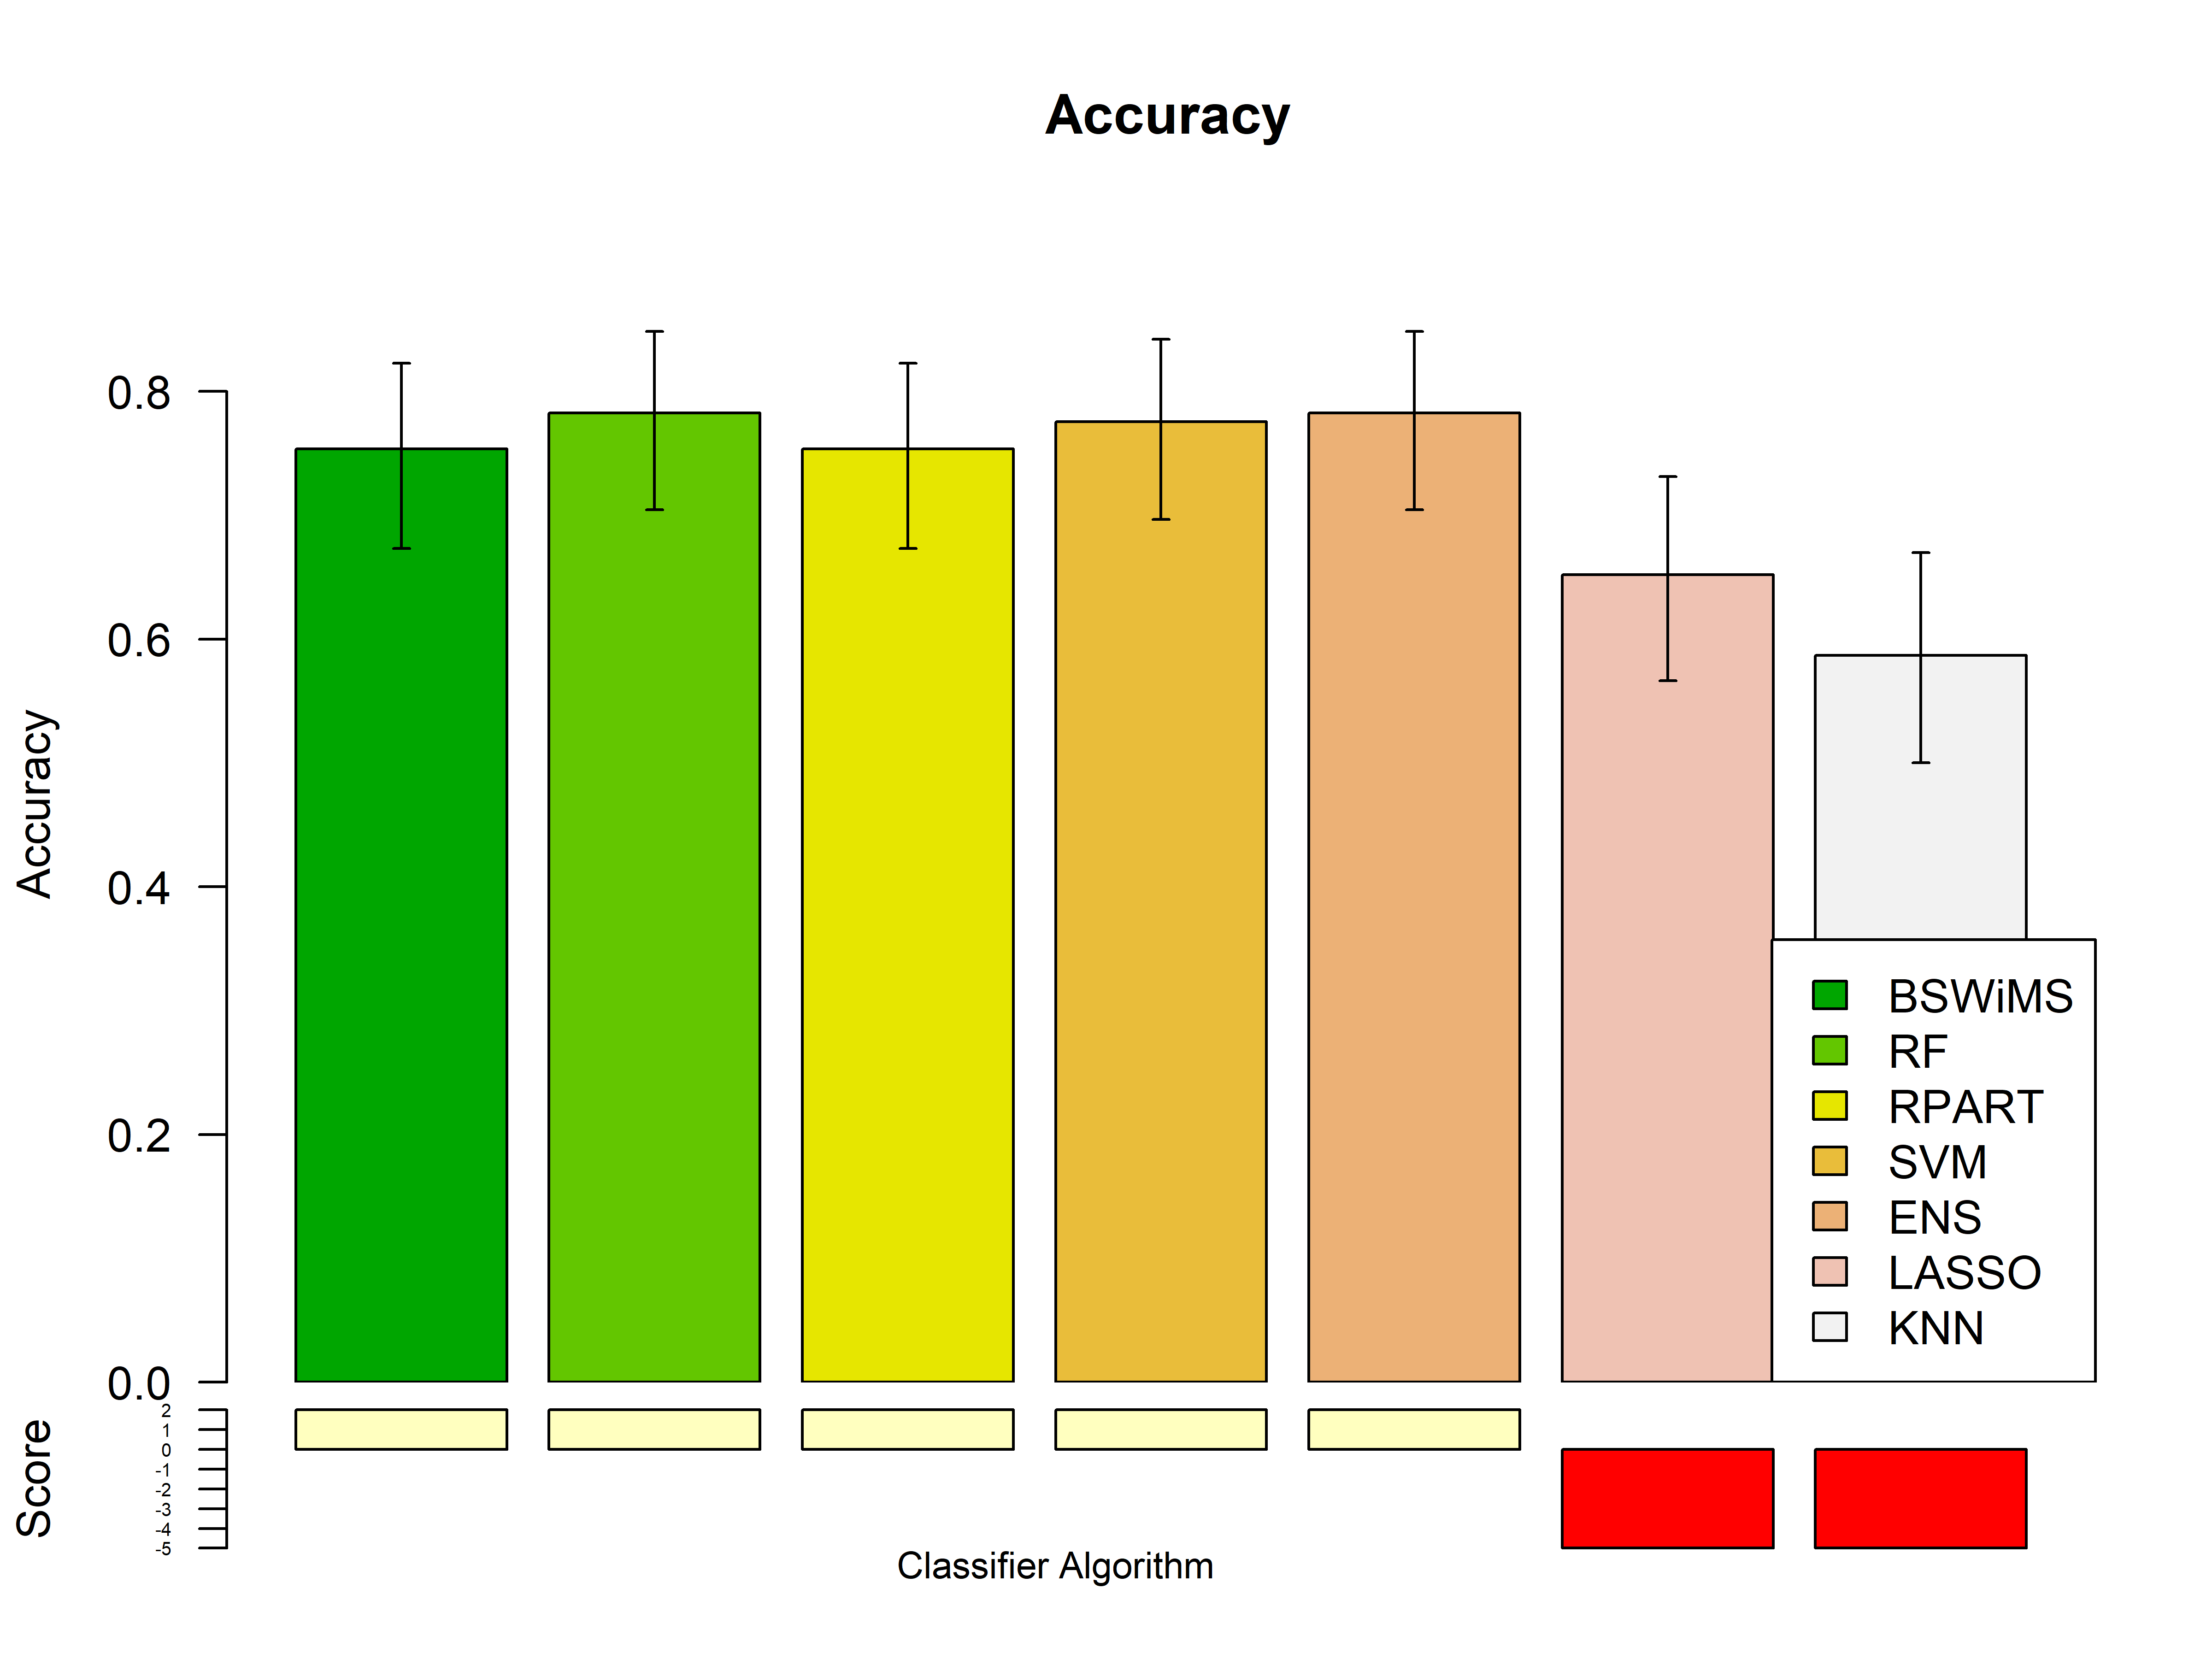
\includegraphics[width=5in,height=2in]{images/results/fresaAccVal.png}}
\centerline{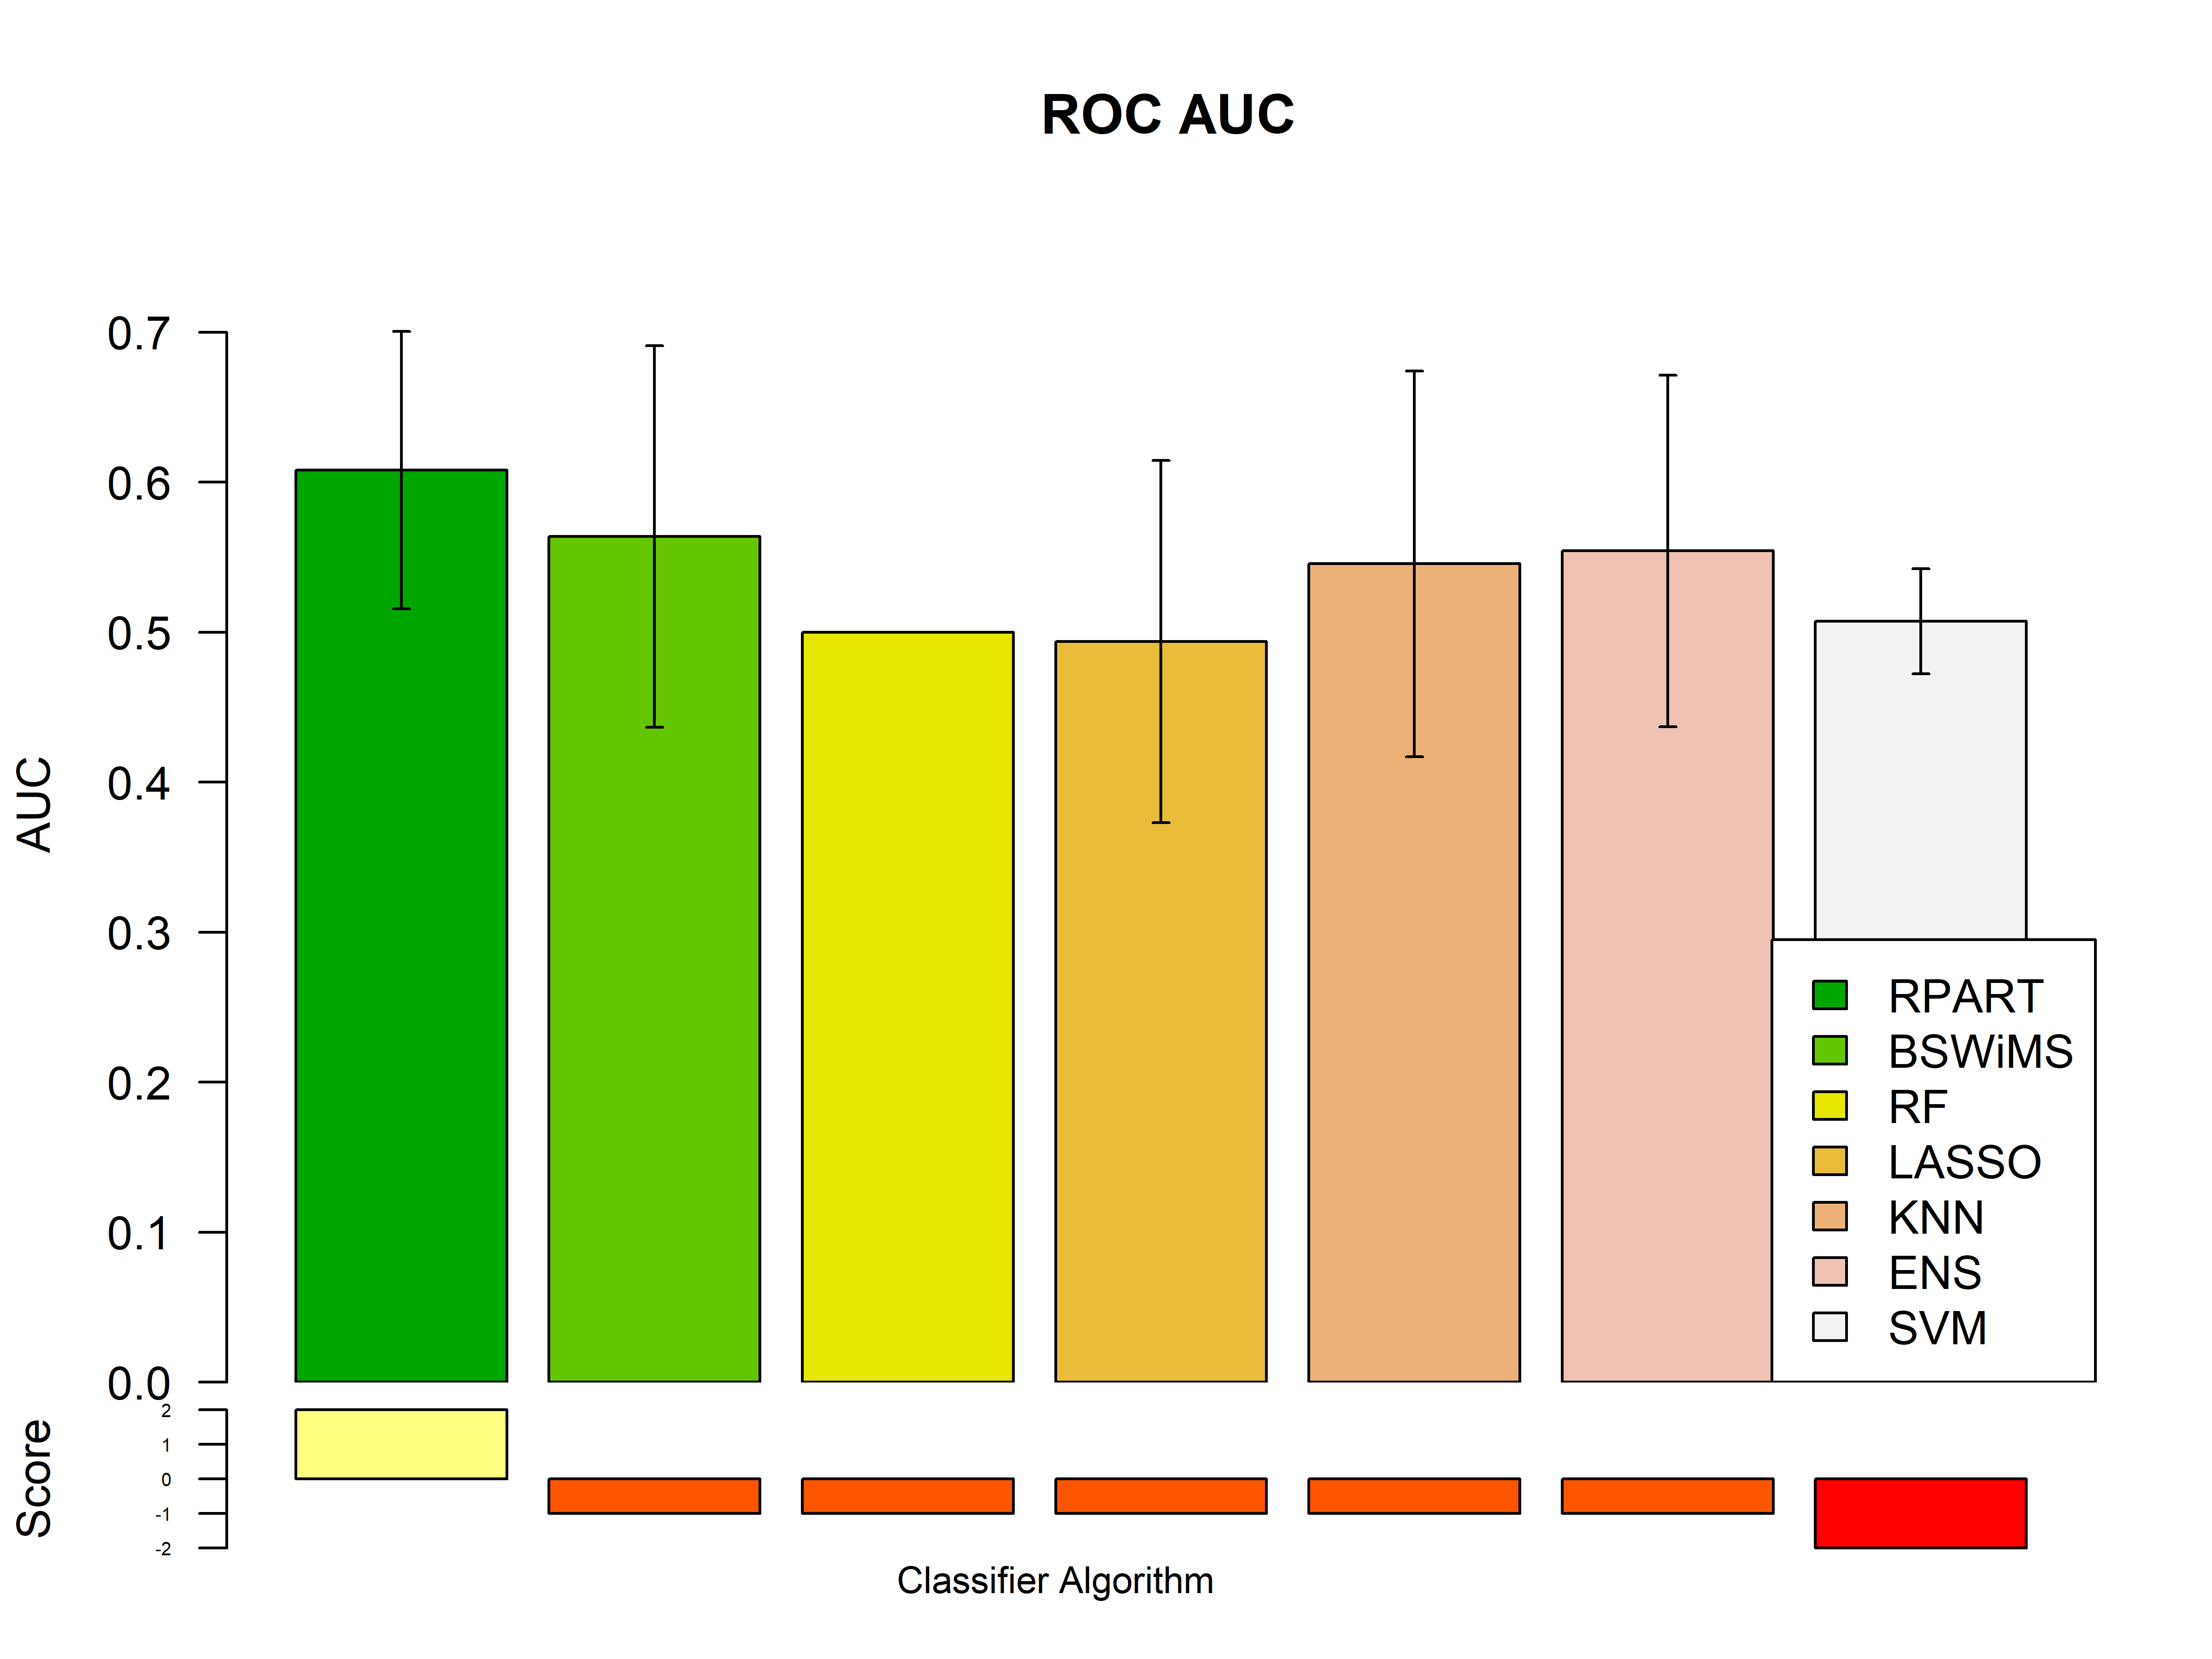
\includegraphics[width=5in,height=2in]{images/results/fresaAUCVal.png}}
\caption{{\bf Validation Balanced Error, Accuracy and AUC of the FRESA.CAD Benchmark classifiers} 
Comparison between the Balanced Error, Accuracy and AUC Score obtained using the different classification methods of the FRESA.CAD Benchmarking with the validation dataset for the Cross-validation and using the top 1,000 SNPs as input}
\label{fig26}
\end{figure}

   
\begin{figure}[!ht]
\centerline{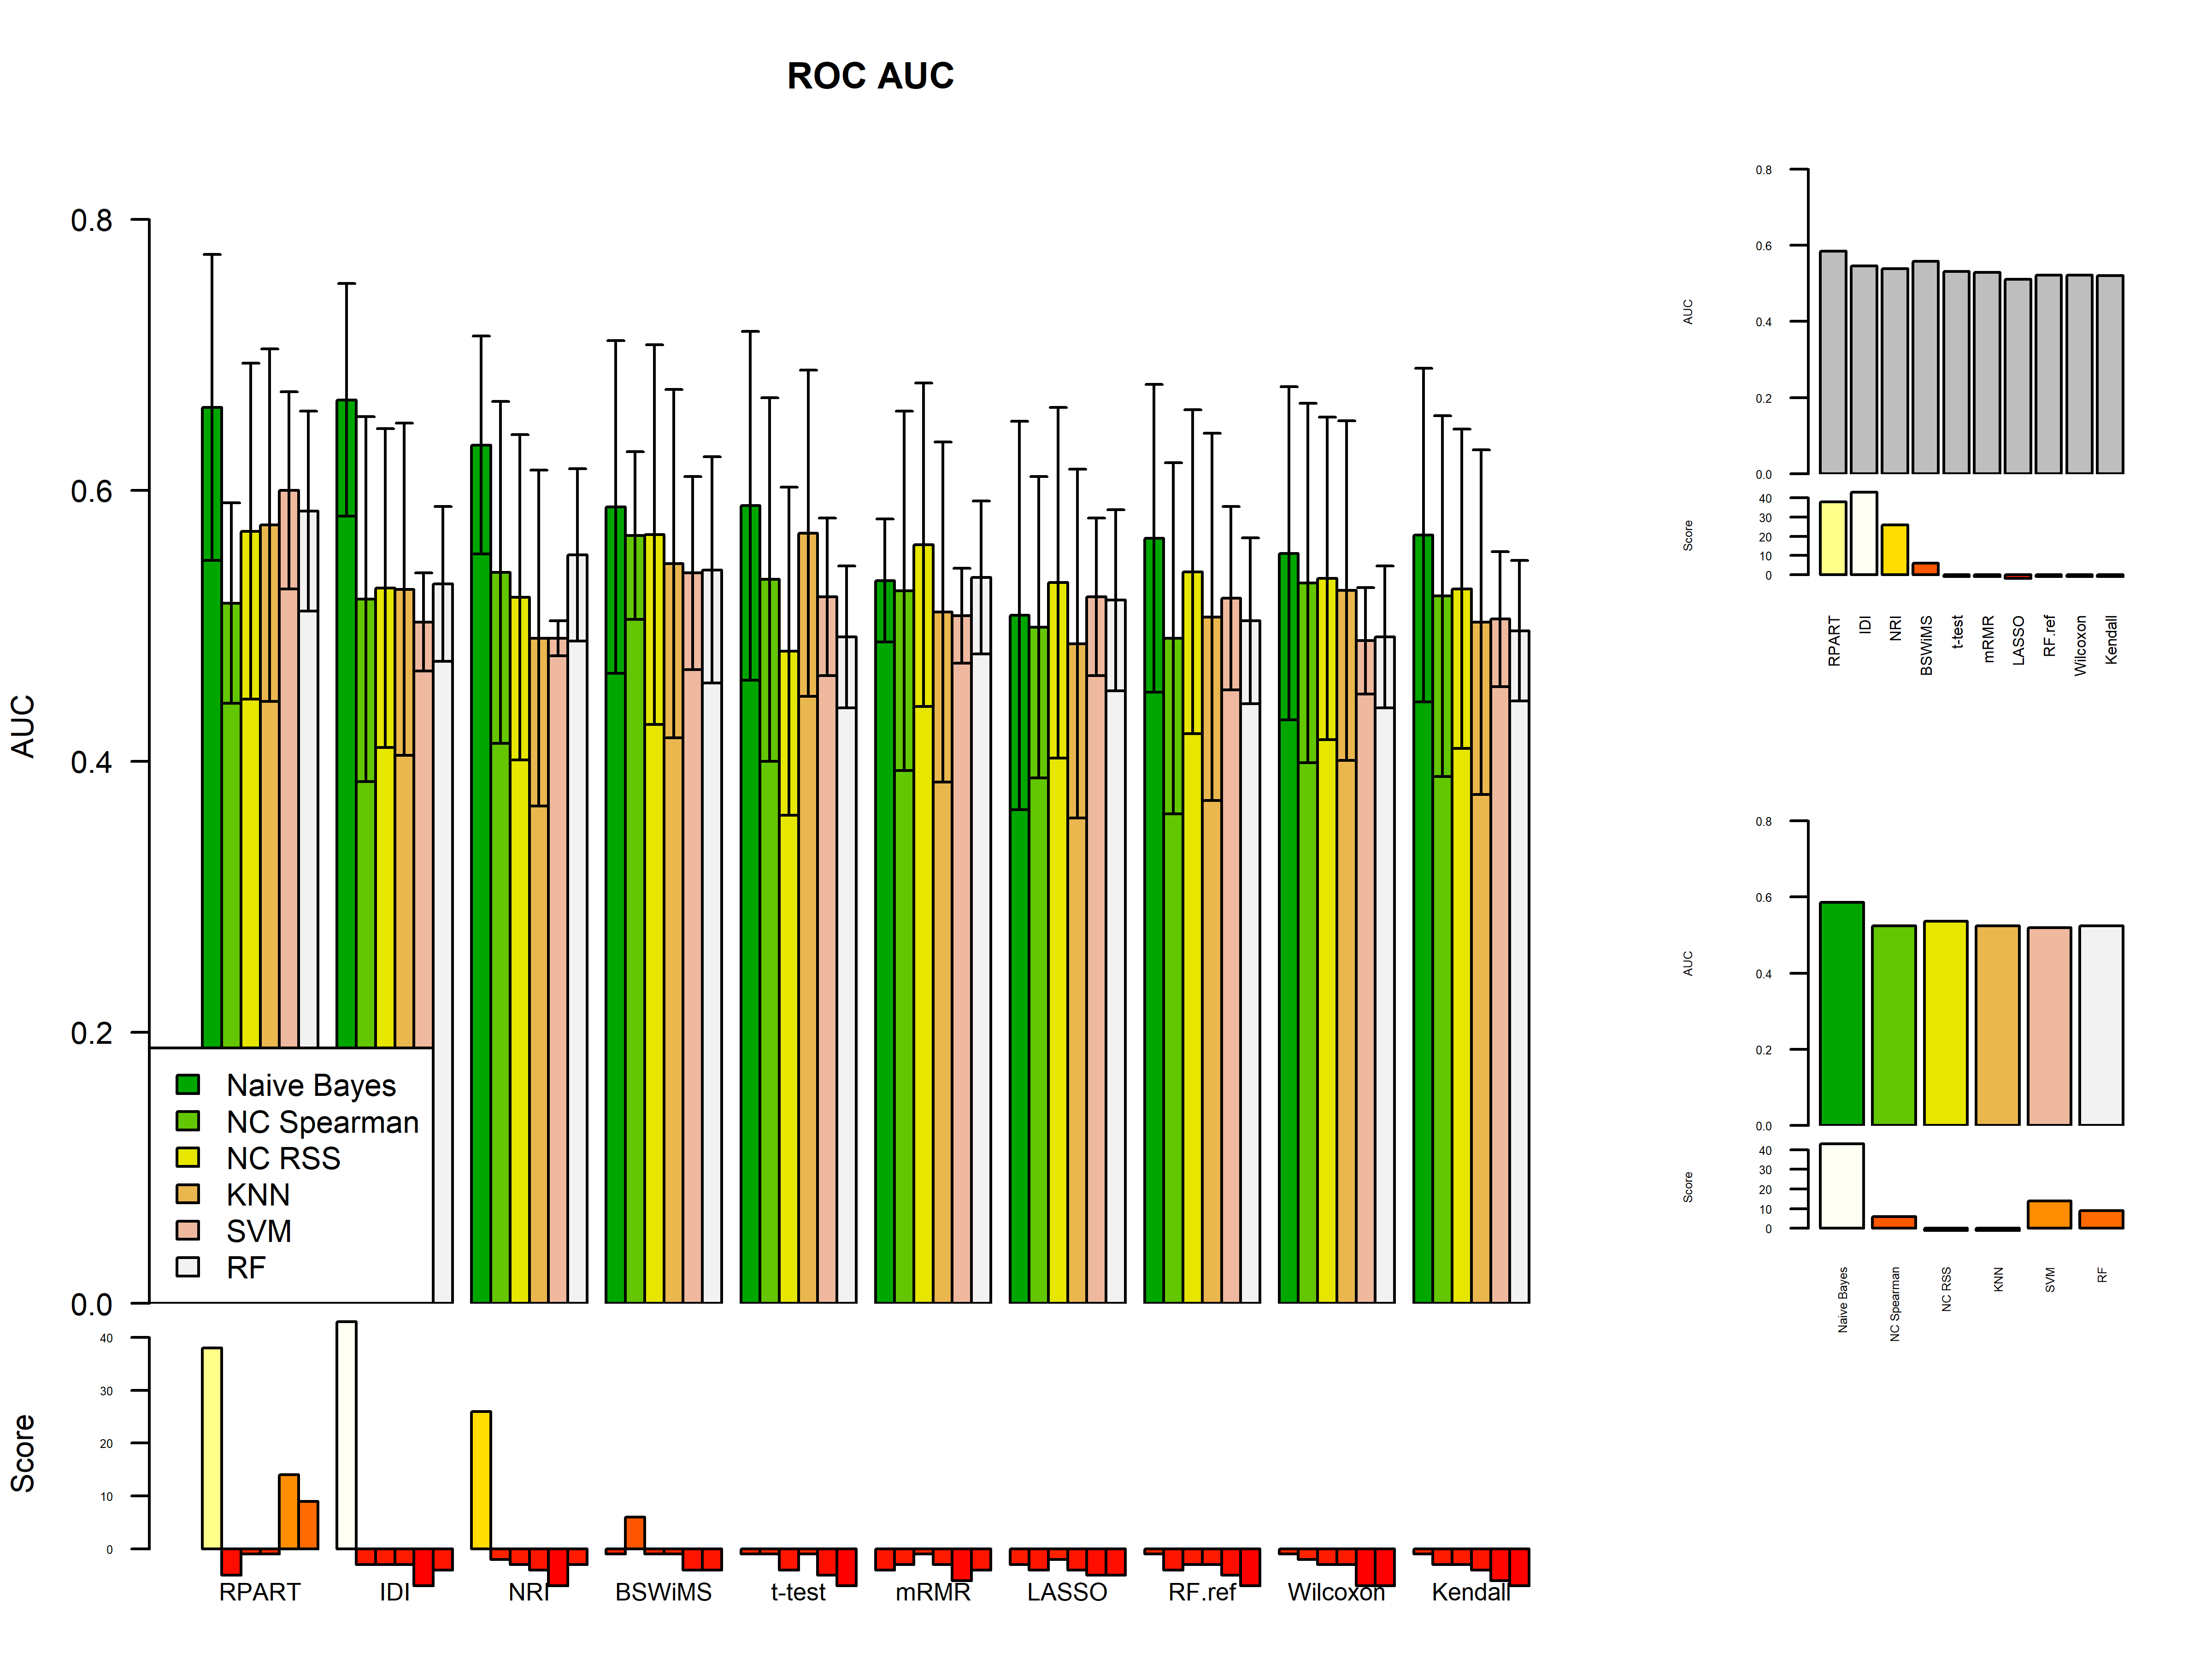
\includegraphics[width=5in,height=2in]{images/results/fresaConcVal.png}}
\centerline{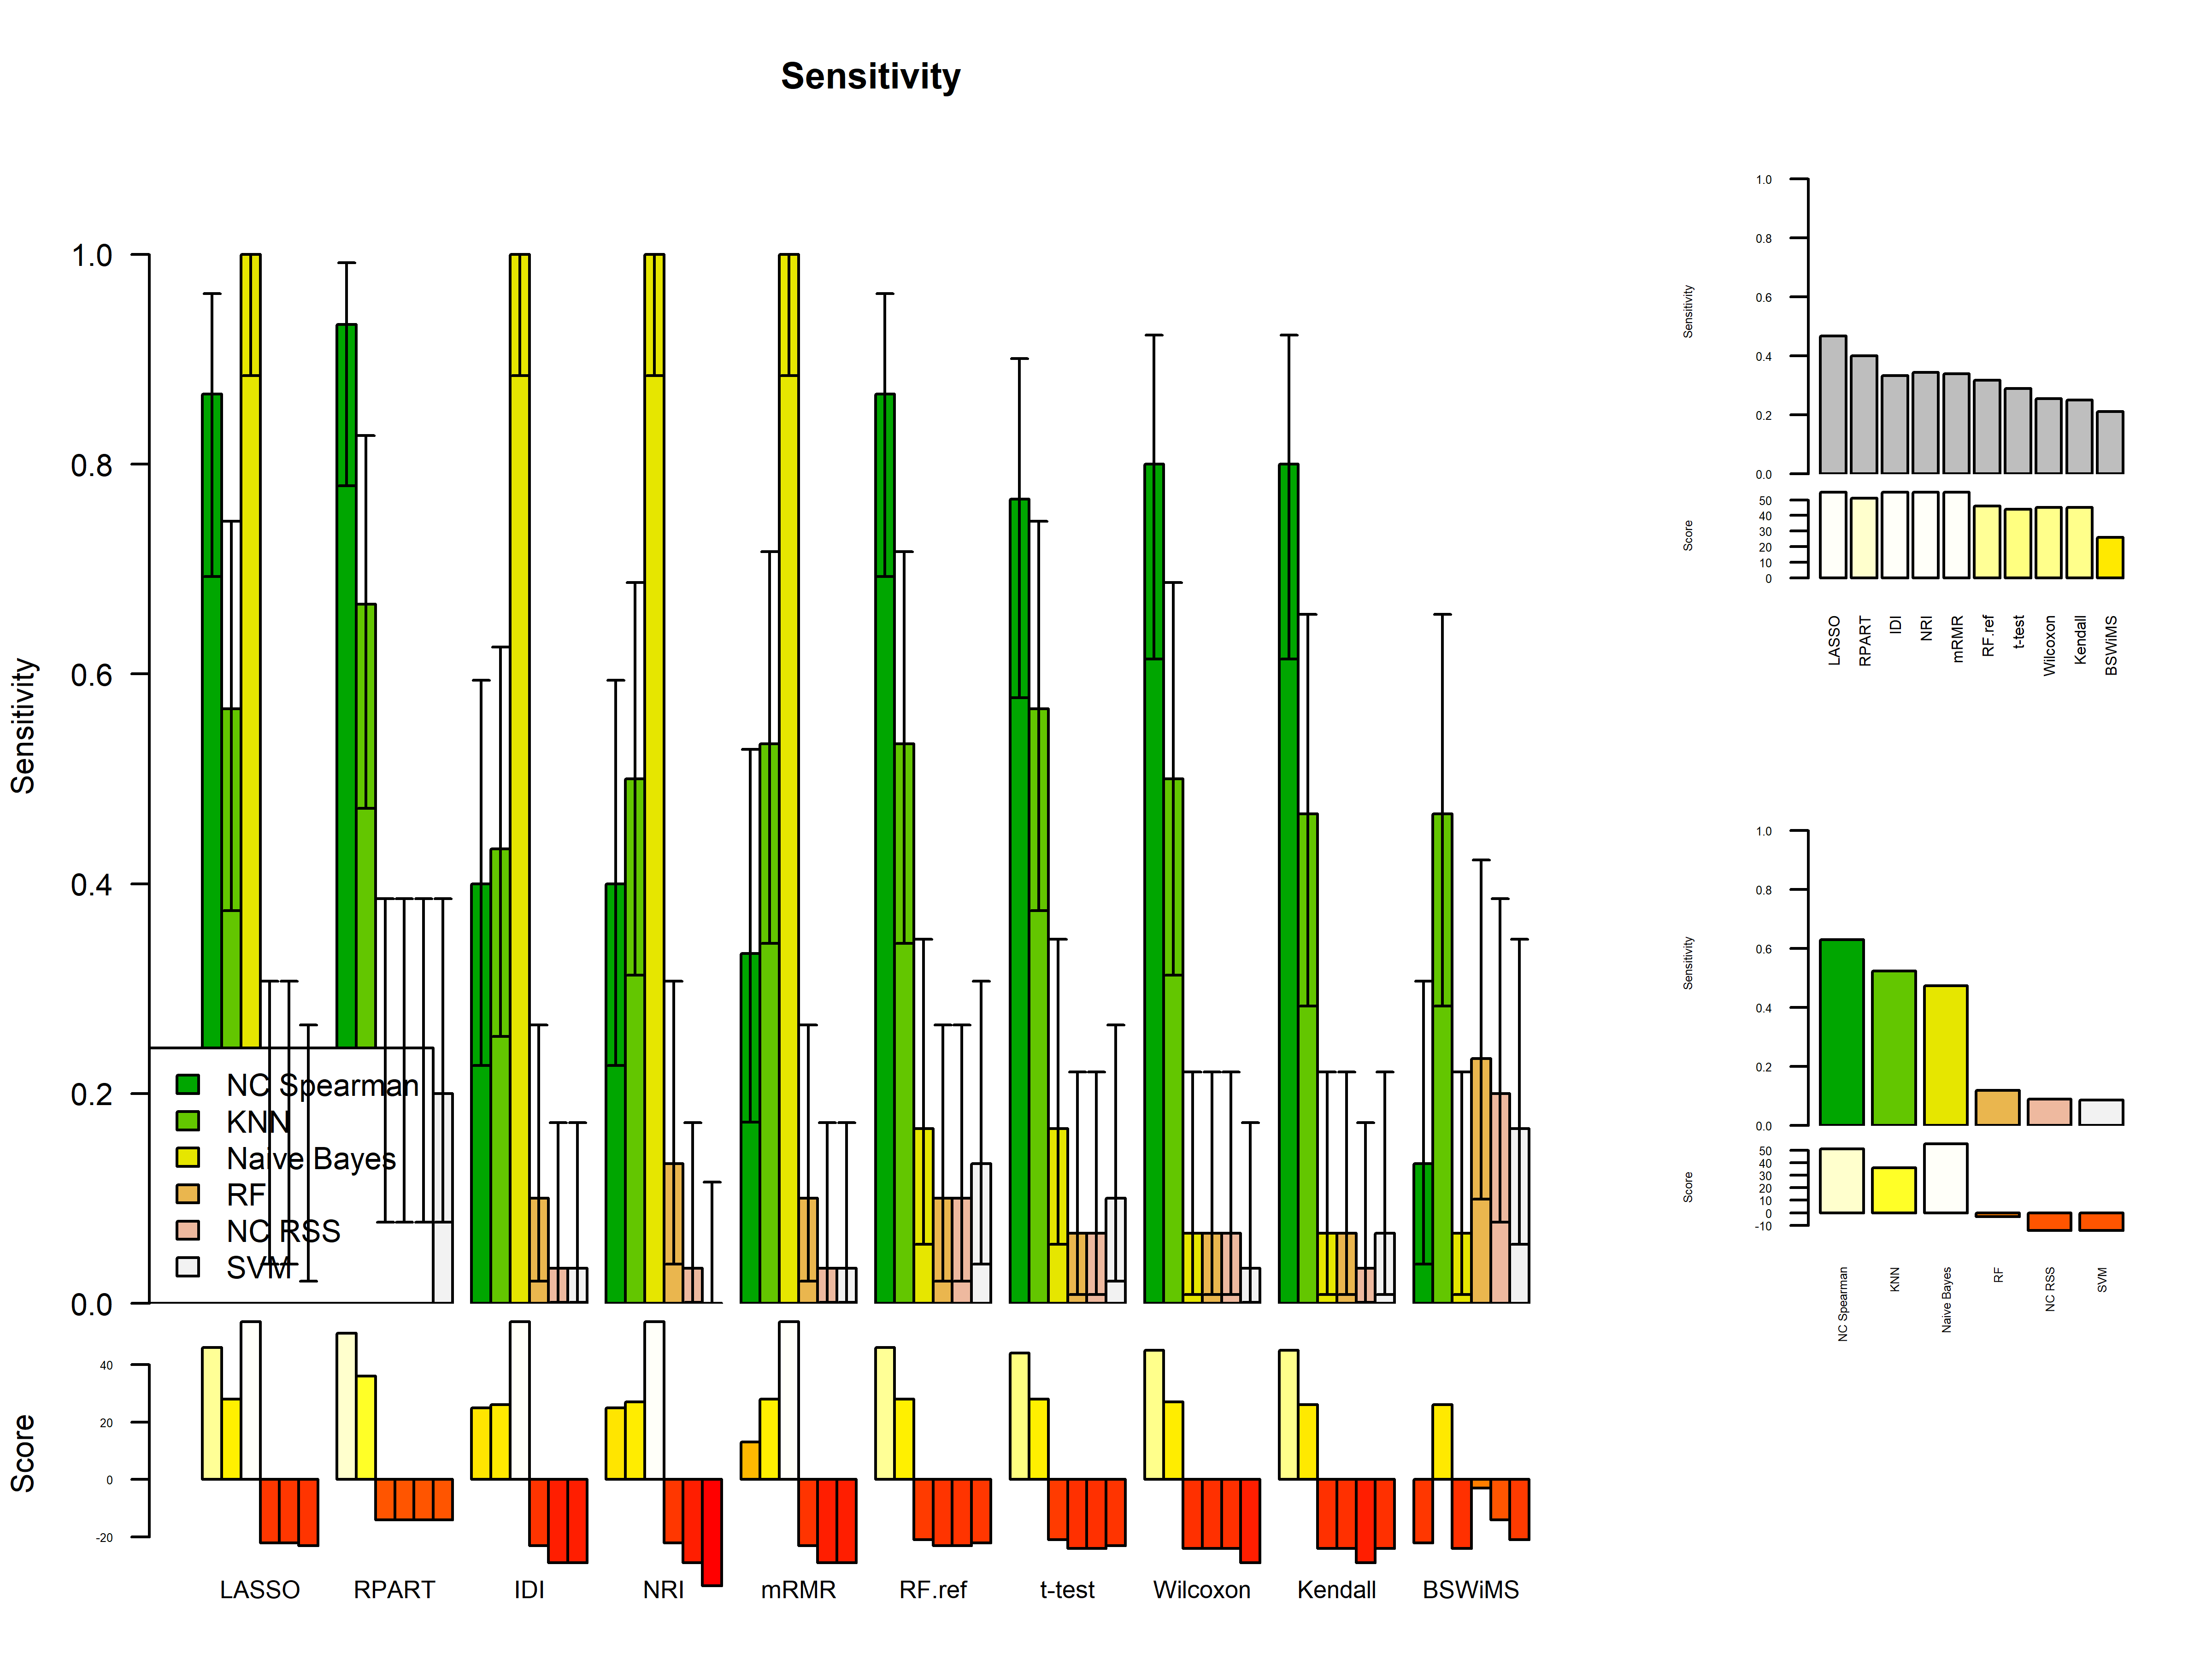
\includegraphics[width=5in,height=2in]{images/results/fresaSensVal.png}}
\centerline{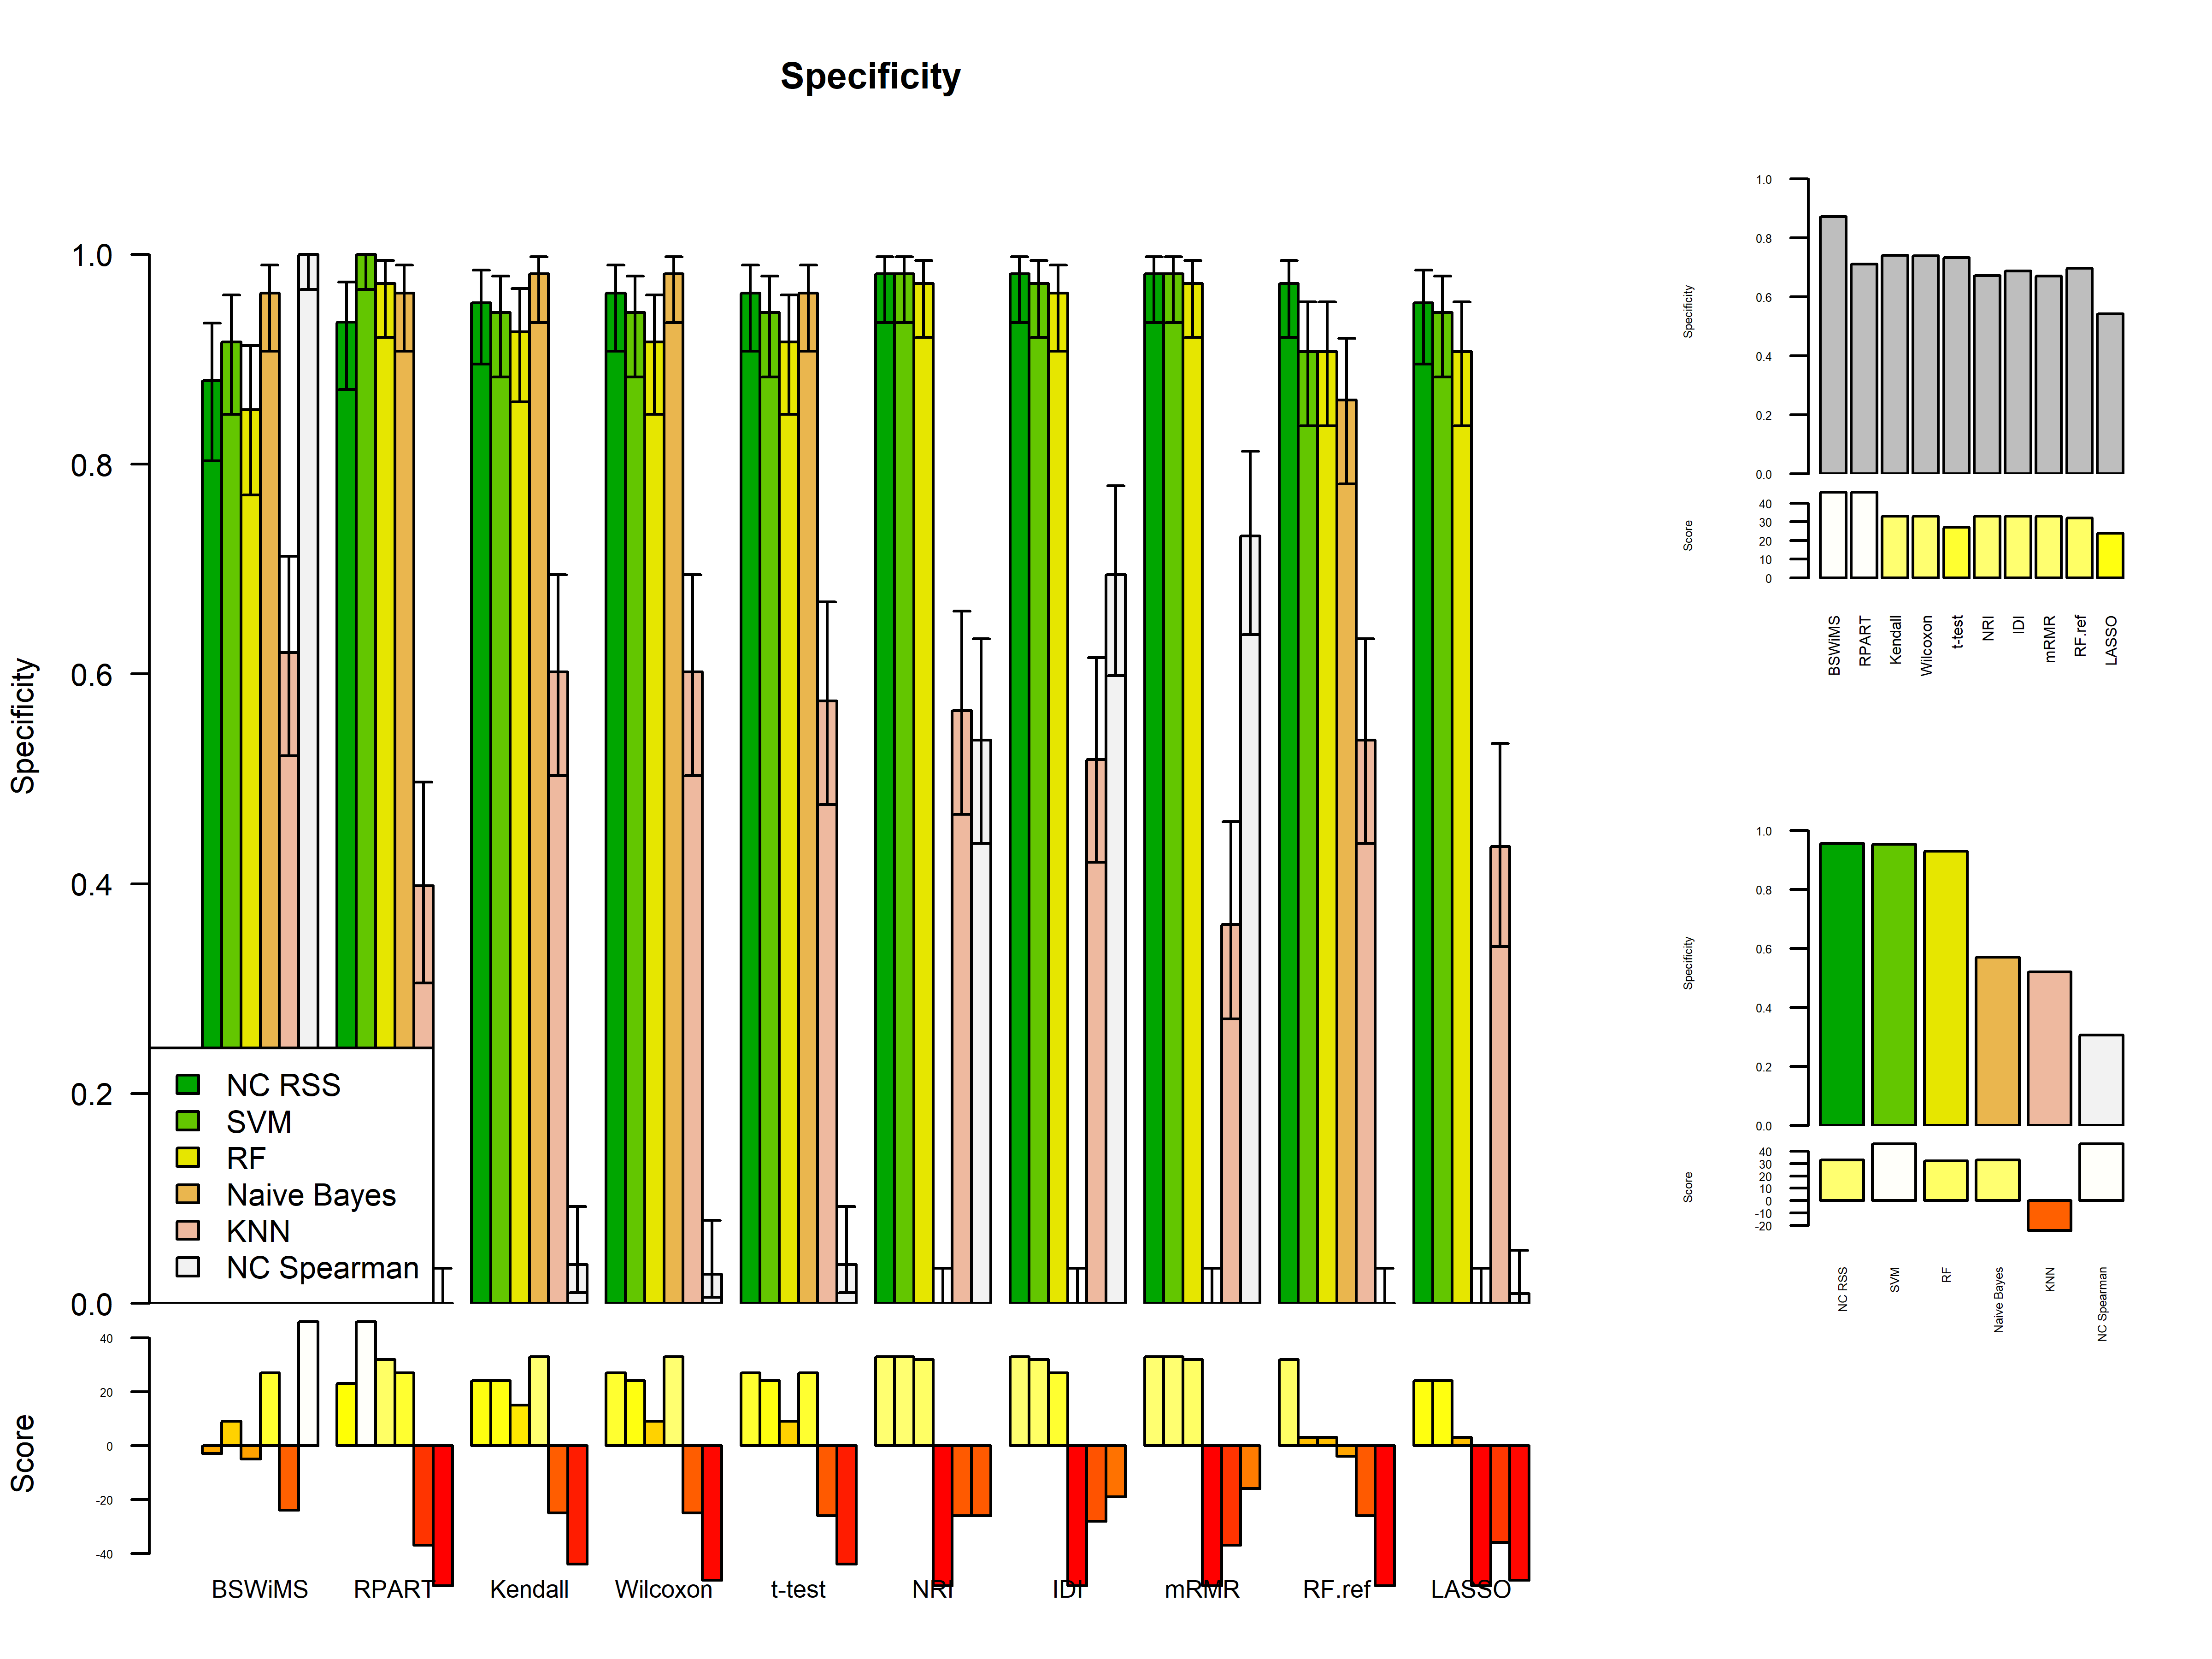
\includegraphics[width=5in,height=2in]{images/results/fresaSpecVal.png}}
\caption{{\bf Validation ROC AUC, Sensitivity and Specificity of the FRESA.CAD Filter combinations} 
Comparison the ROC AUC, Sensitivity and Specificity Score obtained using the different combinations of classification methods plus filters of the FRESA.CAD Benchmarking with the validation dataset for the Cross-validation and using the top 1,000 SNPs as input}
\label{fig22}
\end{figure}
\clearpage
When performing the Meta-Analysis to detect candidate SNPs a much different situation happens than before. As shown in Figure 4.23 there are much more SNPs being selected with a frequency higher than 0.1, which could be interpreted as having less certainty of the SNPs that provide a stronger classification probability. Table 2 seems to back this too, as there are multiple . Coincidentally, the SNPs selected previously are not the same ones as before. APOE $\epsilon4$ is definitely the top marker again, but only rs6448799 appears on both besides APOE $\epsilon4$, thus leading to believe that the SNPs being selected could be either statistical coincidences due to the small amount of samples, or behaving differently now that there is no IGAP information leakage. RPART also appears to not include APOE $\epsilon4$ and still achieve good results, which is certainly odd. As described before, the ROC AUC scores are higher than the actual results obtained in the experiment by far, which reinforces the reason why these scores are not equivalent to the previous ones.
\begin{figure}[!ht]
\centerline{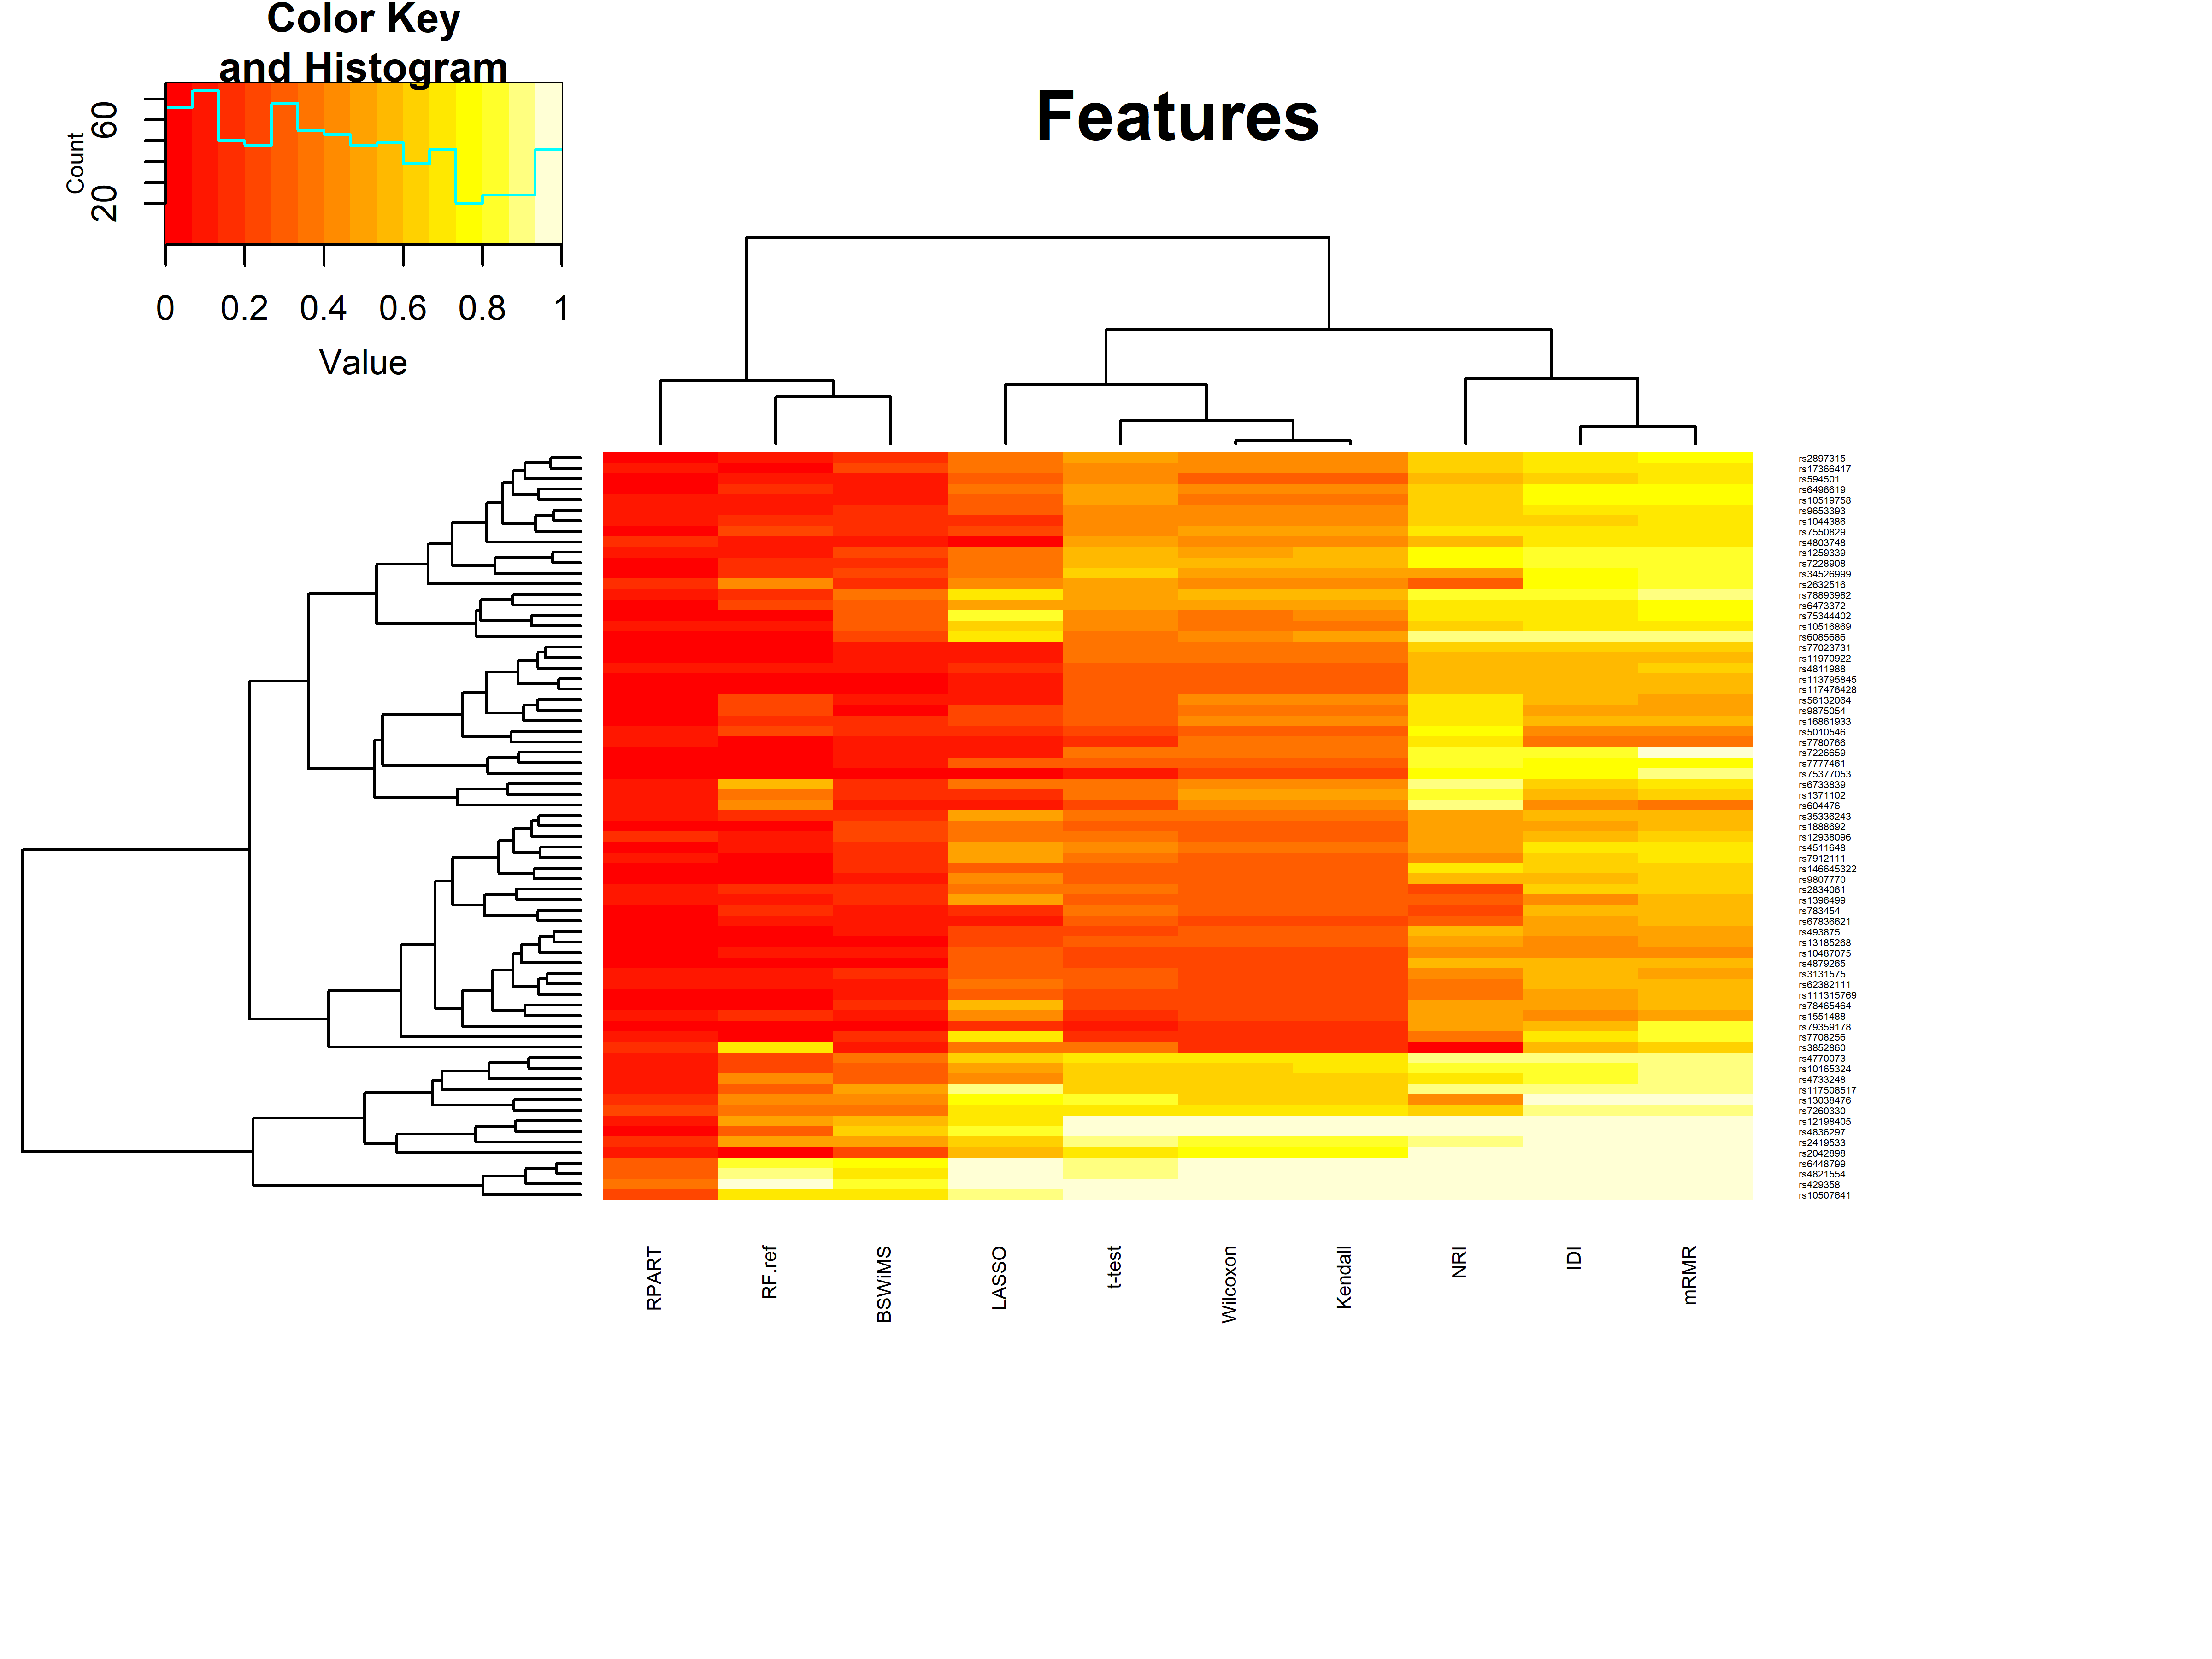
\includegraphics[width=4in]{images/results/fresaSNPsVal.png}}
\caption{{\bf Validation SNPs chosen more than 10\% of the time as features of the FRESA.CAD Benchmark} 
Heatmap of the main SNPs being chosen across all the classifiers. The Y axis are the main SNPs being selected while the X axis represents the different classifiers of the FRESA.CAD Benchmarking with the validation dataset for the Cross-validation and using the top 1,000 SNPs as input}
\label{fig23}
\end{figure}

\begin{table}[ht!]
    \begin{center}
        \begin{tabular}{|c|c|c|c|}
        \hline
        \textbf{SNP}   &  \textbf{ROC AUC} &  \textbf{WILCOX} &  \textbf{FREQ} \\ \hline
rs429358   &	0.684 &	0.0436 &	0.91 \\ \hline
rs6448799  &	0.6614 &	0 &	0.815 \\ \hline
rs4821554	&	0.6537 &	1e-04 &	0.874 \\ \hline
rs7260330	&	0.6383 &	0.0027 &	0.667 \\ \hline
rs10507641	&	0.637 &	0 &	0.797 \\ \hline
rs4733248	&	0.6349 &	0.0052 &	0.581 \\ \hline
rs13038476	&	0.6318 &	0 &	0.627 \\ \hline
rs2419533	&	0.6304 &	0.0013 &	0.716 \\ \hline
rs34526999	&	0.6228 &	0.025 &	0.445 \\ \hline
rs2632516	&	0.6185 &	0.02 &	0.387 \\ \hline
        \end{tabular}
    \end{center}
  \caption{Top  SNPs selected as important features for the Validation dataset}
  \label{topsnps2}
\end{table}

\clearpage
\section{LDPred-funct}

The results of the LDPred-funct are not very interesting. As an intermediate metric the $h^2$ score is calculated, which in rough terms  gives the heritability of the disease, in this case the result is a value of 0.06 based on the IGAP statistics which basically means that the heritability component of the disease statistically found is not very high, this result is consistent with other analysis done previously. As a contrast, the phenotype height is shown to be 0.58 in the LDPred-funct paper.

LDPred-funct then returns an $r^2$ value of 0.025. A more layman representation is to say that the PRS calculated by LDPred-funct can explain 42\% of the expected heritability limit, and that the method can explain 3\% of the variance shown in the disease. This is a low value and is also represented in the Polygenic Risk Score. When using it to classify between cases and controls the PRS assigns every sample in the ADNI validation dataset as a case. This means that the ROC score is 0.50 and for classification purposes is not useful.

Now, this result and low heritability calculation are at odds with the APOE $\epsilon4$ statistics. This result is mainly due to the small size of the validation dataset as well as the complexity of Alzheimer's Disease in terms of genetic heritability. It could be that with a much larger validation dataset or using a larger summary statistic for Alzheimer would give more accurate results. Additionally, as the diagnosis of Alzheimer's is post-mortem the summary statistics could also be skewed. But the values obtained are consistent with the results of other complex diseases such as Type 2 Diabetes, Cron's Disease and Schizophrenia \cite{Consortium2009}, which further reinforces the point that AD is highly complex, polygenic and multifactorial.

\section{Discussion}


Previous research on the early detection of late-onset Alzheimer's disease have relied on a variety of clinical biomarkers for disease prediction \cite{Alexiou2017}. The efficacy of experimental treatments and palliative interventions rely heavily on the early detection of the disease \cite{Dufouil2018}. Unfortunately, clinical biomarkers such as beta amyloid and tau proteins are correlated with disease progression. Therefore, their usefulness for the early detection of the disease remains controversial.

The etiology of LOAD is likely to be motivated by both environmental and genetic components. However, the genetic component seems to a major determinant as the heritability of the disease has been estimated to be $\sim$ 80\% \cite{Raghavan2017}. Therefore, genetic testing hold the potential to provided sufficiently accurate predictions of the disease using genetic data exclusively. Unfortunately, the genetic variants with associations with LOAD discovered by GWAS studies are only capable to explain a fraction of this genetic component (33\%). Therefore, methodologies that account for this missing heritability are required to achieve better predictions \cite{Escott015} \cite{Escott2017}.

In this thesis, it is proposed the use of deep neural networks and machine learning  for predicting late-onset Alzheimer's disease from genetic data. This Thesis' hypothesis postulated that the use of a large number of genetic variants would allow us to improve the classification performance of the proposed model. It is expected of the deep learning model to create hierarchical features with the potential to account for the missing heritability of the disease.

Experimental results indicate that classification performance of $\sim$ 65\% AUC can be achieved with the proposed model. In comparison, the use of the APOE $\epsilon4$ gene with the ADNI dataset gives a predictive score of 0.61\% ~ 0.62\% on the Cross-Validation and 56\% ~64\% on the Split Validation depending on the method. Most importantly, the experiments reported here suggest that an increasing number of genetic variants as predictors hold the potential to contribute to improve the predictive capabilities of the proposed model providing that a sufficiently large number of samples are available. 


The deep learning models in particular suffered from overfitting the training data in the experiments (and obtaining a score of 98\%~100\%). Through the use of dropout, normalization and regularization this was controlled but the main way overfitting can be avoided is through the use of a larger sample size . The deep learning models consist of a large number of possible parameters, and as such with a low number of samples the tendency to overfit is larger. By increasing the size of the dataset the overfitting problem will reduce and the model will have a lower variance. Furthermore, another issue with the current dataset is that the number of predictors\/features outnumber the number of samples. This creates a problem where each individual feature could present low variance within the samples to be of statistical use. 

In the majority of experiments reported here, random forest produced better results that deep learning models possibly because of these issues. However, according to empirical observations on the performance of deep learning models in these experiments (especially the simulations) , it is expected the latter to outperform the former as more data becomes available. In general, deep learning models have shown to scale the performance better than other machine learning models with increasing amounts of data \cite{Goodfellow2016}.

\newpage
Simulated models of purely genetic diseases tend to show the models perform as expected, by analyzing a greater number of markers as well as a greater number of samples they are able to obtain better performance. The models were never able to learn with perfect accuracy the underlying causes for the simulated disease, which is to be expected considering that the disease is spread out through 12,000 genes. This could also show what is happening with other diseases, where the factors could be even greater. This does show the value of Machine Learning for Genomic analysis and specifically the importance of using big datasets that can give the full spectrum of information usable to predict precisely.

Data-augmentation in turn did not give results informative enough to validate its use on the first case with using the full dataset, although for the case where only the independent validation set was used by doing Data Augmentation the models were able to perform better than the models where there existed no data augmentation. This could be either because the number of validation data versus the training data is too low and by doing the Data-Augmentation the data set increases sufficiently to increase the performance, or because the validation samples are sufficiently different in terms of gene distribution that the learned features are not useful in the testing set. The second idea is supported by the results obtained in the meta-analysis using FRESA.CAD. 

For the case of the models tested with the FRESA.CAD Benchmark the Ensemble method is able to explain 70\% of the expected genetic component for the given full ADNI Cohort. It can also be seen that the different methods selected as features SNPs which have been reported in the literature to have a correlation with Alzheimer, thus showing that the algorithm is consistent with the results previously found and has a medical basis. The reduced cohort for the independent validation score would then just explain 33\% of the genetic variation, but this could be due to the balance problem as well as the low data set size. The FRESA.CAD Benchmark seems to be a promising tool for Genomics analysis and finding candidate markers.
 
 LDPred-funct was found to have results that were lacking in predictive power but which are slightly consistent with other reported complex diseases. This validates yet again with another approach the difficulty being faced with predicting Alzheimer's Disease. The results on small datasets appear to show that for small samples or test sets the Machine Learning models are better in the prediction task than more statistical approaches to the disease. Given much larger datasets one could expect the LDPred-funct algorithm to perform better than most machine learning algorithms.
 \newpage
 LOAD prediction is a challenging problem. In effect, the etiology and the genetic architecture of the disease remain unexplained. Moreover, accurate diagnosis of the disease is still an open problem. Therefore, labeled datasets including confirmatory diagnosis are not currently available. This data would be critical for the construction of accurate predictive models. Further research and development of models could open avenues to increase the certainty of the diagnosis that could in the long run increase the precision of predictive models.

In addition, it is unclear whether or not there are useful genetic variants that account for the transition from mild cognitive impairment to LOAD. According to recent studies, currently available LOAD polygenic scores are not capable to predict mild cognitive impairment to LOAD progression \cite{Lacour2016}. Therefore, alternative models are also required for the accurate prediction of disease progression.
		%\include{chapters/content/discussion} 
		% ***************************************
% ***************************************
\chapter{Conclusions and future work} \label{conclusions}
% ***************************************
% ***************************************

In this chapter, the conclusions derived from the results 
(chapter \ref{results}) are shown in section \ref{section_conclusions}. 
Additionally, future work and suggestions to extend the current investigation are shown in 
section \ref{section_future_work}. 

% ***************************************
\section{Conclusions} \label{section_conclusions}
% ***************************************



This thesis presented the hypothesis that the existence of multiple genes with low effect sizes contribute to the total risk of developing LOAD. Using a genomics-based Machine Learning and Deep Learning approach seems to be a viable alternative for Alzheimer's Disease prediction due to AD being a complex, polygenic, multifactorial disease. The methods seems to be suited to analyze the model where multiple genes spread out across the entire genome each contributing with a low risk percentage give a compound genetic risk of developing the disease. Previous research has consistently proven that Alzheimer's does have a genetic component which is complex in nature and thus using these models makes sense. The hypothesis was tested using computational experiments using the ADNI dataset where deep learning and machine learning models with multiple genetic variants as input.

The main objectives were accomplished with certain caveats: The desired score of achieving a ROC AUC score above 0.65 was accomplished both with Support Vector Machines and with the FRESA.CAD Benchmark, with the detail that these results were obtained using the whole set of the ADNI dataset. Using the simulated dataset the different algorithms were shown to perform with good performance, especially when considering an increase in the number of SNPs used as inputs coupled with an increase of the dataset size. This seems to prove the hypothesis that these Machine Learning and Deep Learning algorithms are suited for genomics problems in general. Data-augmentation was proven to be of use in one of the two subsets of data, whereas in the other did not consistently improve which begs further experiments to correctly validate its use. The performance of the models did indeed work with clinical and lossy data, as all samples had a degree of missing SNPs and were all from human patients from the ADNI Study. The dataset appears to have enough diversity to do some types of analysis and decent models were extracted from the data, but the sample size does limit the capacity of the models to learn and the statistical confidence in the results that were obtained and as such an alternate dataset is desirable. All the models appear to support the previous work done with respect to the APOE $\epsilon4$ gene, which was shown to outperform every other variant by a fair margin, but other possible variants were shown to have a correlation with the disease and could be investigated further in the future.

This thesis has shown the applicability of Machine Learning and Deep learning algorithms to predict the risk of developing Alzheimer's Disease using only the genome of an individual which would be incredibly powerful to prevent this disease at an early age. The current limitations primarily due to the complexity of the disease and the dataset limitations are also shown as avenues of improvement. This thesis is also inclined to show how Deep Learning and Machine Learning are powerful tools suited by their nature to analyze and use a multitude of genes which could be used in a variety of complex diseases similar to Alzheimer's Disease. The results tend to show that the two most important factors to ensure a good performance with these types of models to create a Polygenic Risk Scores as an alternative to statistical PRS are the use of more SNPs coupled with a larger sample size. In fact the current trend points toward the large-scale application of these methods with the ever increasing demand for individual genome sequencing and the availability of much larger datasets, both with private companies and from research groups. This shows a very promising future to fully understand the complexity of the human genome and its interactions through the use of advanced Deep Learning algorithms with the full breadth of the entire human population as learning basis, and could enable highly powerful and precise health procedures at a very early stage.

% ***************************************
\section{Future work} \label{section_future_work}
% ***************************************

There are some research questions arising from this work which can be improved upon with future work. One of the main limitations of multiple methods analyzed is that they perform better the more samples that are given to the algorithms to learn from, as well as to validate. Thus the main improvement that can be done is to increase the dataset size, having more variance and statistical power for the different methods, ensuring that datasets which are independent are used to avoid removing samples. Another challenge faced by this thesis is the complexity of the diagnosis of LOAD, using a larger dataset allows filtering out more specific samples that could reduce the uncertainty with respect to the disease diagnosis, and as more datasets are available further certainty due to the passing of the years is also generated (Such as the ADNI 3 protocol). The final problem surrounding the dataset is the class balance, given a much larger dataset or complimentary datasets from multiple sources then the balance can be adjusted more easily without losing too much of the dataset size, and the unbalance will be less pronounced the more data samples there are.

With respect to the simulation methodology the choice of having different versions or characteristics of multiple parameters could help characterize different types of complex diseases, this could be used to obtain a more accurate performance baseline from which to test the methods. The Data Augmentation procedure could also be improved upon, by using the data from a much larger study or by refining the methodology so that the data is even more closely related to the underlying statistical distribution. The choice of odds ratio and the way of handling the Linkage Disequilibrium are also factors that could be modified.

Another interesting avenue of research is the use of hand-selected markers with larger weights directly instead of allowing the learning methods to automatically select the importance of these markers. The model would then try to fit the other SNPs that have not been reported in the literature, but would ensure those that have been proved to have an impact will always be maintained.

The FRESA.CAD method can also be optimized to include the clumping procedure to have it done per Cross-validation instead of having to perform it before the algorithm to ensure that the statistical samples are in LD. This could allow the use of the complete dataset instead of the independent validation dataset. Furthermore, this could allow the usage of a direct statistical analysis instead of performing the GWAS-based filtering beforehand.

Furthermore, the candidate genes being selected as the top variants by the FRESA.CAD benchmark can also be explored to see if some marker in Linkage Disequilibrium is already reported, or if it is not to check the biological pathways that could validate the markers as being biochemically valid and not only statistical.

Finally, the LDPred-funct algorithm could be run with a much larger sample and the performance of it would be expected to considerably improve in a way as to make it worthwhile.

This thesis thus has proven to be innovative and pushed the state of the art regarding Alzheimer's Disease prediction using multiple machine learning and deep learning methods from a genomics perspective and hopes to serve as inspiration to further develop these types of models in the hope that Alzheimer's Disease can be solved for future generations.


	%%%%%%%%%%%%%%%%%%%%%%%%%%%%%%%%%%%%%%%%%%%%%%%%%%%%%%%%%%%%%%%%%%%%%%%%%%%%%%%%
	% Load bibliography style :
	% ieeetr is IEEE format
		\bibliographystyle{ieeetr}
	% Load bibliography file :
		\bibliography{bibliography/references}
	%%%%%%%%%%%%%%%%%%%%%%%%%%%%%%%%%%%%%%%%%%%%%%%%%%%%%%%%%%%%%%%%%%%%%%%%%%%%%%%%
	% add vita
		% ***************************************
% ***************************************
\chapter*{Vita} \label{Vita}
% ***************************************
% ***************************************

\addcontentsline{toc}{chapter}{Vita}

%%%%%%%%%%%%%
\begin{center}
\end{center}
%%%%%%%%%%%%%

\authorName\ is a a graduate candidate for a MSc.in Computer Engineering at ITESM campus CEM. His work focuses in Deep Learning approaches for Medical diagnostics from a Genetic perspective. His main area of application is Alzheimer's Disease and other neurological disorders. He enjoys reading, especially fantasy and science fiction, playing video games, designing electronic circuits and traveling.

%%%%%%%%%%%%%
\begin{center}
\end{center}
%%%%%%%%%%%%%

\begin{center}
	{@}\thesisYear\ by \authorName \\
	All rights reserved
\end{center}

\null
\vfill

% insert footnote with package details
\begin{center}
	\packageDetails
\end{center}

\begin{center}
    \textbf{\thesisDate} 
\end{center}



	%%%%%%%%%%%%%%%%%%%%%%%%%%%%%%%%%%%%%%%%%%%%%%%%%%%%%%%%%%%%%%%%%%%%%%%%%%%%%%%%
\end{document}


